% This is the Reed College LaTeX thesis template. Most of the work
% for the document class was done by Sam Noble (SN), as well as this
% template. Later comments etc. by Ben Salzberg (BTS). Additional
% restructuring and APA support by Jess Youngberg (JY).
% Your comments and suggestions are more than welcome; please email
% them to cus@reed.edu
%
% See http://web.reed.edu/cis/help/latex.html for help. There are a
% great bunch of help pages there, with notes on
% getting started, bibtex, etc. Go there and read it if you're not
% already familiar with LaTeX.
%
% Any line that starts with a percent symbol is a comment.
% They won't show up in the document, and are useful for notes
% to yourself and explaining commands.
% Commenting also removes a line from the document;
% very handy for troubleshooting problems. -BTS

% As far as I know, this follows the requirements laid out in
% the 2002-2003 Senior Handbook. Ask a librarian to check the
% document before binding. -SN

%%
%% Preamble
%%
% \documentclass{<something>} must begin each LaTeX document
\documentclass[11pt,singlespacinge,twoside]{reedthesis} %,headseplin
% Packages are extensions to the basic LaTeX functions. Whatever you
% want to typeset, there is probably a package out there for it.
% Chemistry (chemtex), screenplays, you name it.
% Check out CTAN to see: http://www.ctan.org/
%%
\usepackage{flipbook}
\usepackage{pgf}
\usepackage{graphicx,latexsym}
\usepackage{lastpage}
\usepackage{amsmath}
\usepackage{amssymb,amsthm}
\usepackage{longtable,booktabs,setspace}
\usepackage{chemarr} %% Useful for one reaction arrow, useless if you're not a chem major
\usepackage[hyphens]{url}
% Added by CII
\usepackage{hyperref}
\usepackage{lmodern}
\usepackage{float}
%\floatplacement{figure}{H}
% End of CII addition
\usepackage{rotating}

% Next line commented out by CII
%%% \usepackage{natbib}
% Comment out the natbib line above and uncomment the following two lines to use the new
% biblatex-chicago style, for Chicago A. Also make some changes at the end where the
% bibliography is included.
%\usepackage{biblatex-chicago}
%\bibliography{thesis}


% Added by CII (Thanks, Hadley!)
% Use ref for internal links
\renewcommand{\hyperref}[2][???]{\autoref{#1}}
\def\chapterautorefname{Chapter}
\def\sectionautorefname{Section}
\def\subsectionautorefname{Subsection}
% End of CII addition

% Added by CII
\usepackage{caption}
\captionsetup{width=5in}
% End of CII addition

% \usepackage{times} % other fonts are available like times, bookman, charter, palatino

% Syntax highlighting #22

% To pass between YAML and LaTeX the dollar signs are added by CII
\title{\textbf{Mechano -- Chemical Feedback Loops \linebreak During Vertebrate Organ Development}}
\author{\textbf{David Kleinhans}}
% The month and year that you submit your FINAL draft TO THE LIBRARY (May or December)
\date{Frankfurt am Main, 2019}
\division{Entwicklungsbiologie der Vertebraten}
\advisor{Prof.~Dr.~Sven Klimpel}
\institution{Johann Wolfgang Goethe-Universität}
\degree{\textbf{PhD in Biology}}
%If you have two advisors for some reason, you can use the following
% Uncommented out by CII
\altadvisor{Prof.~Dr.~Virginie Lecaudey}
% End of CII addition

%%% Remember to use the correct department!
\department{Fachbereich Biowissenschaften}
% if you're writing a thesis in an interdisciplinary major,
% uncomment the line below and change the text as appropriate.
% check the Senior Handbook if unsure.
%\thedivisionof{The Established Interdisciplinary Committee for}
% if you want the approval page to say "Approved for the Committee",
% uncomment the next line
%\approvedforthe{Committee}

% Added by CII
%%% Copied from knitr
%% maxwidth is the original width if it's less than linewidth
%% otherwise use linewidth (to make sure the graphics do not exceed the margin)
\makeatletter
\def\maxwidth{ %
  \ifdim\Gin@nat@width>\linewidth
    \linewidth
  \else
    \Gin@nat@width
  \fi
}
\makeatother

\renewcommand{\contentsname}{Table of Contents}
% End of CII addition

\setlength{\parskip}{0pt}

% Added by CII

\providecommand{\tightlist}{%
  \setlength{\itemsep}{0pt}\setlength{\parskip}{0pt}}

\Acknowledgements{I thank\ldots{}\newline

\noindent my supervisors
\begin{itemize}
\tightlist
\item
  Prof.~Dr.~Virginie Lecaudey
\item
  Prof.~Dr.~Manfred Schliwa
\end{itemize}
\noindent my students
\begin{itemize}
\tightlist
\item
  Dmitri Baulin (M.Sc. Thesis)
\item
  Felix Godron (B.Sc. Thesis)
\item
  Andreas Ebert (B.Sc. Thesis)
\item
  Gelwa Helmand (B.Sc. Thesis)
\item
  Bianca Rodrigues Lima (Master student)
\item
  Ivan Alcantara (Master student)
\end{itemize}
For trust shown in the process, for support and demand. \newline For their patience, engangement and hard work!
\newline\newline
\noindent and my animals, without whom this work would not have been possible.
\vspace{0.2cm}}

\Dedication{These \pageref{LastPage} pages are dedicated to YOU, the \emph{reader}.\newline

The decision to get a PhD for me was not a career option. I chose to be a scientist because \emph{science} because I was motivated by its ideals - autonomy, purity and freedom of presupposition (Aristotle) - to offer a solution to many wronggoings in the world. to to me meant I believed it was a reasonable way, the only way, a better future. Today, even though we are on the verge of becoming a technocracy, society doesn't trust scientific results anymore. This has many reasons.\newline

``Tell the truth. Don't blame people. Be strong. Do your best. Try hard. Forgive. Stay the course.'' - Bush Senior}

\Preface{\begin{quote}
"The most exciting time in the history of developmental biology is right now. Fueled both by new technologies and by new thought from other fields, we are exploding old notions and opening fantastic new horizons in embryology. {[}\ldots{}{]}
\end{quote}
\begin{quote}
Next, let's discuss why developmental biology --- both normal and pathological --- holds such enduring fascination. I see two intertwined explanations. Obviously, it's the ultimate personal creation story, telling each of us both where we came from and how we were constructed. Less obvious, but perhaps more tantalizing for us scientists, is the sheer complexity of the process. A single cell with a single genome can somehow create trillions of cells in hundreds of radically different types, and those cells can organize themselves into a specific form. The scale of this self-organization process is mind boggling, surely the most amazing of emergent properties."
\end{quote}
\begin{quote}
- John B. Wallingford, 2019\footnote{``We Are All Developmental Biologists'', Developmental Cell, Vol.50, Issue 2, Jul 22, 2019}
\end{quote}}
\Abstract{}

	\usepackage{booktabs}
\usepackage{longtable}
\usepackage{array}
\usepackage{multirow}
\usepackage{wrapfig}
\usepackage{float}
\usepackage{colortbl}
\usepackage{pdflscape}
\usepackage{tabu}
\usepackage{threeparttable}
\usepackage{threeparttablex}
\usepackage[normalem]{ulem}
\usepackage{makecell}
\usepackage{xcolor}
% End of CII addition
%%
%% End Preamble
%%
%
\begin{document}

\pagenumbering{arabic} % Make sure a page numbering scheme is explicitly set at the beginning.

  \maketitle

%\frontmatter % this stuff will be roman-numbered
\pagestyle{empty} % this removes page numbers from the frontmatter
  \begin{acknowledgements}
    I thank\ldots{}\newline
    
    \noindent my supervisors
    \begin{itemize}
    \tightlist
    \item
      Prof.~Dr.~Virginie Lecaudey
    \item
      Prof.~Dr.~Manfred Schliwa
    \end{itemize}
    \noindent my students
    \begin{itemize}
    \tightlist
    \item
      Dmitri Baulin (M.Sc. Thesis)
    \item
      Felix Godron (B.Sc. Thesis)
    \item
      Andreas Ebert (B.Sc. Thesis)
    \item
      Gelwa Helmand (B.Sc. Thesis)
    \item
      Bianca Rodrigues Lima (Master student)
    \item
      Ivan Alcantara (Master student)
    \end{itemize}
    For trust shown in the process, for support and demand. \newline For their patience, engangement and hard work!
    \newline\newline
    \noindent and my animals, without whom this work would not have been possible.
    \vspace{0.2cm}
    \begin{center}
      \includegraphics[width=0.5\textwidth]{figure/05-Appendix/DSC07341.png}
    \end{center}
  \end{acknowledgements}
%\mainmatter % here the regular arabic numbering starts
%\pagestyle{fancyplain} % turns page numbering back on

  \hypersetup{linkcolor=black}
  \setcounter{tocdepth}{2}
  \tableofcontents

  \listoftables

  \listoffigures
  \vfill
  \begin{center}
    \textbf{Disclosure}\\
    {Unless otherwise noted, all figures in this manuscript are an expression of my own creative achievement. Similarities between molecule, protein and signalling models exist and are based on well-known textbooks such as Lodish et al., Molecular Cell Biology, 5th Edt. and Scott F. Gilbert et al., Developmental Biology 11th Edt.}
  \end{center}
  \begin{dedication}
    These \pageref{LastPage} pages are dedicated to YOU, the \emph{reader}.\newline
    
    The decision to get a PhD for me was not a career option. I chose to be a scientist because \emph{science} because I was motivated by its ideals - autonomy, purity and freedom of presupposition (Aristotle) - to offer a solution to many wronggoings in the world. to to me meant I believed it was a reasonable way, the only way, a better future. Today, even though we are on the verge of becoming a technocracy, society doesn't trust scientific results anymore. This has many reasons.\newline
    
    ``Tell the truth. Don't blame people. Be strong. Do your best. Try hard. Forgive. Stay the course.'' - Bush Senior
  \end{dedication}
\mainmatter % here the regular arabic numbering starts
\pagestyle{fancyplain} % turns page numbering back on

\hypertarget{zusammenfassung}{%
\chapter*{Zusammenfassung}\label{zusammenfassung}}
\addcontentsline{toc}{chapter}{Zusammenfassung}

something

\hypertarget{summary}{%
\chapter*{Summary}\label{summary}}
\addcontentsline{toc}{chapter}{Summary}

something

\hypertarget{list-of-abbreviations}{%
\chapter*{List of Abbreviations}\label{list-of-abbreviations}}
\addcontentsline{toc}{chapter}{List of Abbreviations}

\begingroup\fontsize{9}{11}\selectfont
\begin{tabu} to \linewidth {>{\bfseries}c>{\centering}X>{\raggedright\arraybackslash}p{10cm}}
\toprule
\textbf{Index} & \textbf{Abbreviation} & \textbf{Elaboration}\\
\midrule
\rowcolor{gray!6}  0-9 & 2-/3-D & Two or Three Dimensional\\

 & A.I. & apical index\\

\rowcolor{gray!6}  \multirow[t]{-2}{*}{\centering\arraybackslash A} & AB & Antibody\\

 & CC & Cell Cluster\\

\rowcolor{gray!6}   & CNN & Convolutional Neural Network\\

\multirow[t]{-3}{*}{\centering\arraybackslash C} & CI & confidence interval\\

\rowcolor{gray!6}   & dpf & days post fertilization\\

\multirow[t]{-2}{*}{\centering\arraybackslash D} & DSH & Dishevelled\\

\rowcolor{gray!6}   & ECDF & Empirical Cumulative Distribution Function\\

\multirow[t]{-2}{*}{\centering\arraybackslash E} & EDF & Extended Depth of Field\\

\rowcolor{gray!6}   & Fgf & Fibroblast Growth Factor\\

 & Fgfr1 & Fgf receptor 1\\

\rowcolor{gray!6}   & FOV & Field of View\\

\multirow[t]{-4}{*}{\centering\arraybackslash F} & FRZ & Frizzled\\

\rowcolor{gray!6}  H & hpf & hours post fertilization\\

 & IJ & ImageJ\\

\rowcolor{gray!6}  \multirow[t]{-2}{*}{\centering\arraybackslash I} & ISH & In Situ Hybridization\\

K & KDE & Kernel Density Estimation\\

\rowcolor{gray!6}   & l.e. & leading edge\\

 & LL & Lateral Line\\

\rowcolor{gray!6}   & LOESS & Locally Weighted Scatterplot Smoothing\\

 & LSFM & Light sheet fluorescence microscope\\

\rowcolor{gray!6}   & LUT & Lookup Table\\

\multirow[t]{-6}{*}{\centering\arraybackslash L} & LMPA & low melting point agarose\\

\rowcolor{gray!6}   & MaxIP & Maximum Intensity Projection\\

\multirow[t]{-2}{*}{\centering\arraybackslash M} & MO & Morpholino\\

\rowcolor{gray!6}   & N.A. & Numerical Aperture3\\

 & NGS & Normal Goat Serum\\

\rowcolor{gray!6}   & NICD & Notch intracellular domain\\

 & NM & Neuromast\\

\rowcolor{gray!6}  \multirow[t]{-5}{*}{\centering\arraybackslash N} & NMII & Non muscle myosin II\\

O & o.n. & over night\\

\rowcolor{gray!6}   & p.Hist & phospho-Histone\\

 & PCR & Polymerase chain reaction\\

\rowcolor{gray!6}   & PFA & Paraformaldehyd\\

\multirow[t]{-4}{*}{\centering\arraybackslash P} & pLLP & Posterior Lateral Line Primordium\\

\rowcolor{gray!6}   & Rock & Rho-Kinase\\

\multirow[t]{-2}{*}{\centering\arraybackslash R} & ROI & Region of Interest\\

\rowcolor{gray!6}   & SBD & Shroom binding domain\\

 & SEM & Scanning Electron Microscopy\\

\rowcolor{gray!6}  \multirow[t]{-3}{*}{\centering\arraybackslash S} & SNR & Signal to Noise Ratio\\

 & TALEN & Transcription activator-like effector nuclease\\

\rowcolor{gray!6}  \multirow[t]{-2}{*}{\centering\arraybackslash T} & TF & Transcription Factor\\
\bottomrule
\end{tabu}
\endgroup{}

\hypertarget{Intro}{%
\chapter{Introduction}\label{Intro}}

\setcounter{page}{1}

\hypertarget{development}{%
\section{Development}\label{development}}

In biology differentiation describes the continuous process of cells dividing and adapting to their ever-changing environment during advancing development, whereby adopting specialized function. Physically a cell represents an open system, which is defined as a unit system able for external interactions. Such a system is therefore not self-dependent and self-sustained, but its current conformation is determined by external interactions. To illustrate this, the cell can the thought of as a marble rolling down a furrowed landscape (figure \ref{fig:wadd}). In this landscape a hill would be a high energy-, a valley a low energy state. The path the marble will take is determined by the furrows in the landscape, since it would always prefer a valley. However, this landscape is not a static structure but is a one that changes at every instant of time.
\begin{figure}

{\centering 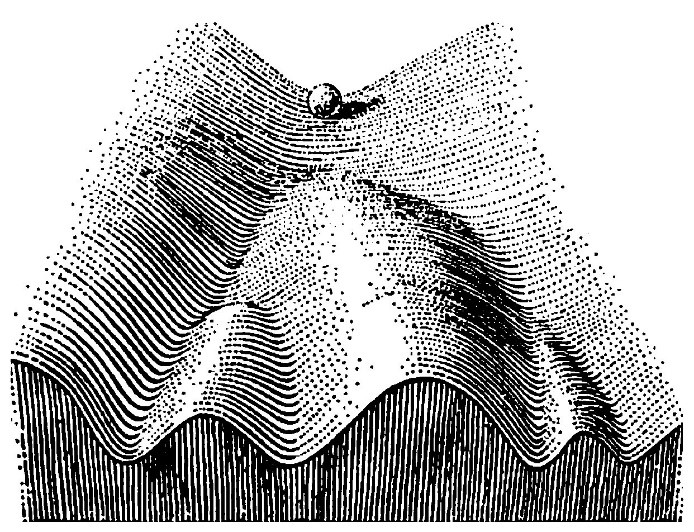
\includegraphics{figures/intro/waddington} 

}

\caption{Waddington's Classical Epigenetic Landscape}\label{fig:wadd}
\end{figure}
For developmental biology, which as a scientific discipline originates from embryology, the central interest is to understand how inanimate matter can form such complex structures we see in living matter at different levels of organismal hierarchy while ensuring a robust developmental plan. Using the marble analogy, studying developmental biology can be thought of tracking multiple cells as they roll down the valley while observing and testing how interactions between them might change their fate. The basic questions arising from this interest are
\begin{itemize}
\tightlist
\item
  How do tissues arise from a population of cells?
\item
  How do organs form from tissues?
\item
  Why do organs form at their particular location?
\item
  How do migrating cells know whether they reached their destination?
\item
  How is growth controlled and how do body axes form?
\end{itemize}
\hypertarget{cell-types}{%
\subsection{Cell Types}\label{cell-types}}

In animals there are two basic types of cells.
\begin{enumerate}
\def\labelenumi{\arabic{enumi}.}
\tightlist
\item
  Epithelial cells, which can form strong bonds between each other and thereby are able to exert forces upon each other to achieve complex architectures.
\item
  Mesenchymal cells, which do not bond with each other and are more independent.
\end{enumerate}
This however describes only the extremes on a continuous scale. A cell is not a binary system but can show characteristics of both extremities, e.g.~during Epithelial to Mesenchymal transition (EMT), a bidirectional process whereby epithelial cells can gain migratory and invasive properties and \emph{vice versa}.

A cells identity on this continuum is determined by
\begin{itemize}
\tightlist
\item
  The cells genome, which reflects its repertoire of molecular machinery (proteins) and therefore determines its competence to react to internal and external cues.
\item
  The cells micro-environment, which has a \emph{physical} (forces, energy) and a \emph{chemical} (signaling molecules, diluents) dimension. A change in the latter usually brings about a reaction in the cell which becomes evident both in expression of genes, which represents the programmatic adaption, and morphologically, which represents the functional adaption.
\item
  The cells shape and incorporation into a tissue, which may modulate the cells affection to its micro-environment (e.g.~certain regions of the cell can be more or less exposed, or it can be more or less tightly packed, tuning its susceptibility to forces and signals).
\end{itemize}
With rising numbers of cells and differentiated tissue a shape and body axes begin to emerge that for the earliest developmental stages is highly similar across certain phyla and only begins to diversify at later developmental stages (figure \ref{fig:heak}), which reflects our evolutionary ancestry. This principle was first formulated by Ernst Haeckel as the biogenetic rule (\emph{1}), which states that ontogenesis (individual development) recapitulates \emph{phylogenesis} (development of phylum)\footnote{While the biogenetic got refuted in its core (there is no `complete' phylogenesis in ontogenesis). It still can't be neglected that embryogenesis even of evolutionary distant species shows remarkable similarities(\emph{2})}.


\begin{figure}

{\centering 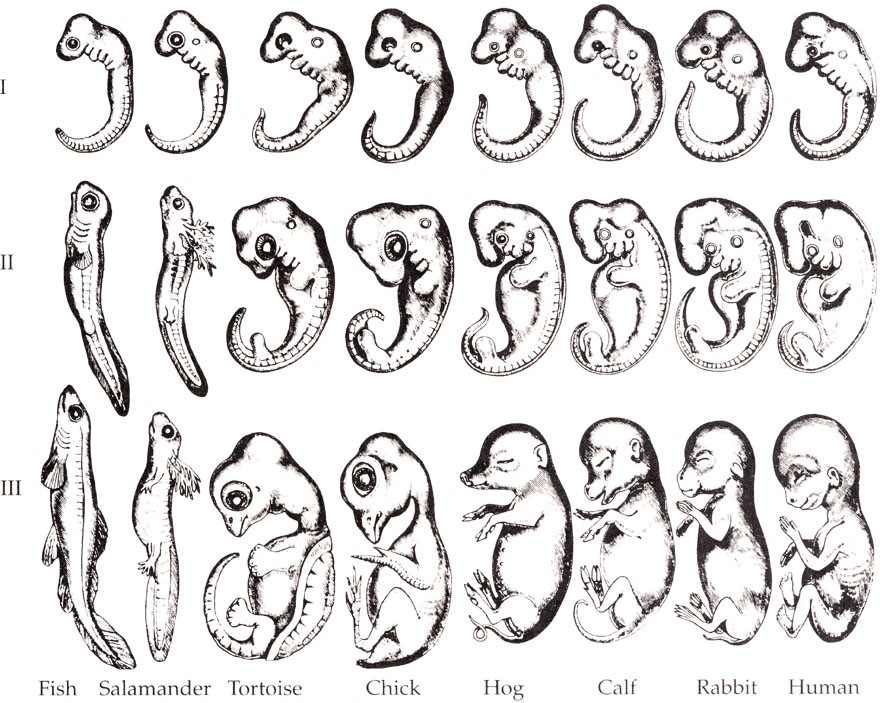
\includegraphics[width=0.75\textwidth]{figures/intro/haekel} 

}

\caption[Ontogenesis across species]{Ontogenesis across species (George Romanes, 1892)}\label{fig:heak}
\end{figure}
\hypertarget{morphogenesis}{%
\subsection{Morphogenesis}\label{morphogenesis}}

Morphogenesis, from the Greek morphê (shape) and genesis (creation)
\begin{quote}
``Beginning of the shape''
\end{quote}
For objects that fulfill a purpose, many times (if not always) their forms (or shapes) are an expression of their function\footnote{Even though the expression Form follows function (\emph{3}) is usually found in design and architecture, it formulates the general idea that any objects form is (or in design should) be shaped by the requirements to it.}. Analyzing the shape of an object can give one information about its function. It is therefore an important feature many different sciences, e.g.~when correlating an organism's size to the climate it lives or when correlating intelligence to the size of an animal's brain. During an organism's development diversification of shape on a cellular level is an important step in breaking symmetry of daughter cells. In order to form a tissue or an organ with a variety of specialized cells, it is important for the single cell to have information about where it is located, what its neighbors are doing, how densely it is packed and what the chemical composition of its surrounding is. This is accomplished by being in constant feedback with its neighbor cells and sensation of its environment. After the information got processed, the cell will react by adjusting the levels of proteins expressed to undergo proliferation or develop specialized structures like cilia or axons.

For a cell, its present shape impacts its further specification by impacting how well it perceives specific signals and the magnitude of signals received and transmitted. E.g. it has been shown that during lateral inhibition (\emph{4}). Shape therefore sets the general framework for cell-cell interaction and follows a\newline

\makebox[\linewidth]{$molecular \longrightarrow cellular \longrightarrow tissue$}
\newline

scale hierarchy, where each scale's output again feeds back to the others (figure \ref{fig:feedb}). E.g. it has been shown that simple changes in cell geometry affect fundamental processes such as cell growth, death, or direction of cell divisions (\emph{5}--\emph{7}).
\begin{figure}

{\centering 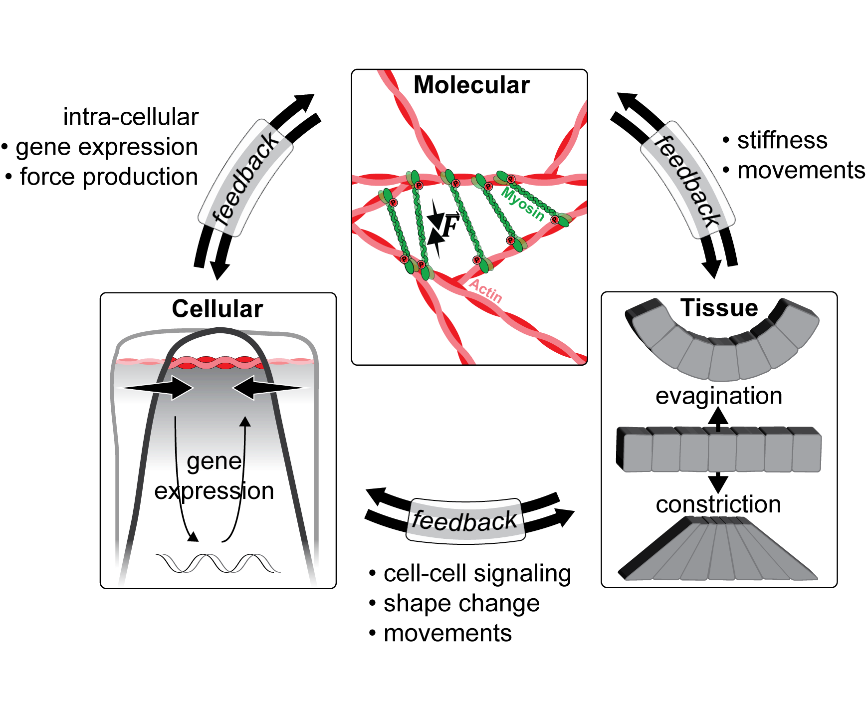
\includegraphics[width=0.75\textwidth]{figures/intro/feedback} 

}

\caption{Form and function feedback loops}\label{fig:feedb}
\end{figure}
\hypertarget{apical-constriction}{%
\subsubsection{Apical Constriction}\label{apical-constriction}}

A defining feature of Epithelial cells is they have a basal- (bottom) to apical (top) polarity. At the basal site, the cell is in contact with the substrate like the extracellular matrix (ECM), apically the cell forms tight connections to its neighbouring cells -- a region called the apical junctional complex (AJC). The AJC encompasses three types of junctions: Adherent junctions (AJ) at the zonula adherens (ZA), tight junctions (TJ) and desmosomes. Around the ZA dense cables of actomyosin are found that, analog to muscle sarcomeres, are able to contract upon RHO‑associated protein kinase (Rock) mediated phosphorylation of the motor protein non-muscle myosin II (NMII) (\emph{8}).

Apical constriction (AC) is a single cell morphogenetic process manifest by an active apical narrowing, making the cell appear bottle or wedge shaped. It is usually coordinated by multiple cells within an epithelial layer that raise forces necessary to deform a tissue.
\begin{figure}

{\centering 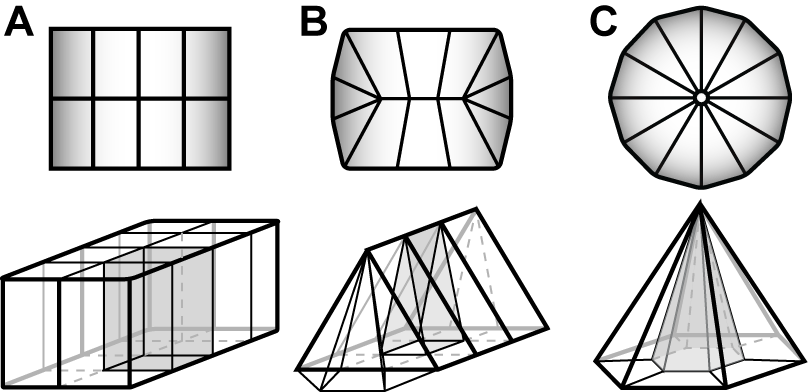
\includegraphics[width=0.75\textwidth]{figures/intro/arrangements} 

}

\caption{Multi-cellular Arrangements}\label{fig:arrange}
\end{figure}
Developmental processes that involve AC are\ldots{}
\begin{itemize}
\tightlist
\item
  Tissue folding and tube formation
\item
  Single cell ingression and EMT
\item
  Gastrulation
\item
  Healing and sealing of embryonic tissue
\end{itemize}
Epithelial rosettes are intermediate structures of radially organized cells within an epithelial tissue whose vertices interface a common center. While the mechanisms of cytoskeletal rearrangements seem to be well conserved, the extracellular cues that lead to rosette formation are less well understood and more diverse.
At least two architectural distinct types of rosettes exist, depending on the tissues polarization (figure \ref{fig:constr}). First, in a planar polarized tissue, several cells converge at a central apico-basal (A-B) line with no shrinkage of the apical surface to form a cylindrical structure. Such rosettes are usually observed during tissue elongation and rather short-lived. In a second scenario, cells converge to a central apical point through AC. This type of rosette is more long-lived and, usually does not resolve but already represents a morphologically pre-mature state of the organ to be formed (\emph{9}).
\begin{figure}

{\centering 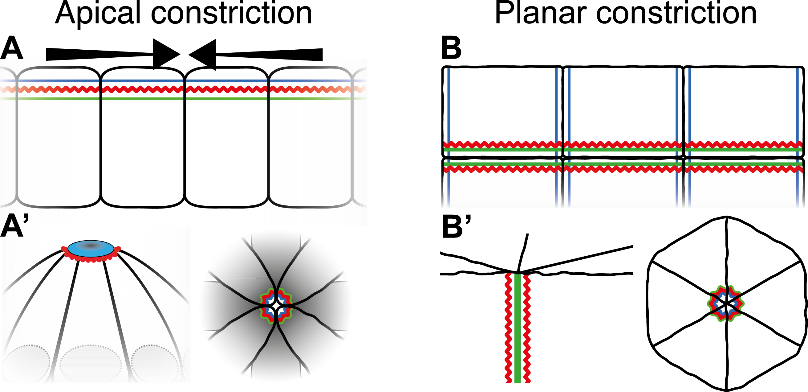
\includegraphics[width=0.75\textwidth]{figures/intro/constriction} 

}

\caption{Modes of Constriction}\label{fig:constr}
\end{figure}
\hypertarget{cell-communication}{%
\subsection{Cell communication}\label{cell-communication}}

To communicate with each other, cells have developed a variety of intercellular communication systems and a complex network of intracellular signal transduction pathways. Some information transfer depends on direct cell-to-cell contact, others rely on freely diffusible ligands that can be sensed by other cells. Each signaling pathway consists of some key regulators of a ligand -- receptor pair that determines their main function. In the following, three pathways are introduced that play major roles in embryonic development.

\hypertarget{wnt-signal-transduction}{%
\subsubsection{WNT Signal transduction}\label{wnt-signal-transduction}}

The word `WNT' is a compound word of \emph{Wingless} and \emph{Int-1}, both of which are important genes during development of \emph{Drosophila melanogaster} (commonly known as fruit fly), where WNT signaling was first studied. WNT is evolutionary conserved with 15 different receptors and co-receptors and plays a major role during embryonic axis formation, body segmentation, organogenesis and stem cell proliferation. Aberrant WNT signaling is involved in diseases like colon cancer, melanoma and neurogenerative diseases (\emph{10}).

Besides this WNT signaling is sub-divided in a canonical (\(\beta\)-catenin\footnote{catenins are regulators of cell-cell adhesion and gene transcription} dependent) and a non-canonical (\(\beta\)-catenin independent) branch. In canonical signaling, WNT ligand binds, together with co-receptor \emph{Lipoprotein Receptor-related Protein} (LRP), to the receptor \emph{Frizzled} (Frz) -- jointly activating protein \emph{Dishevelled} (Dsh). Dsh again inhibits a protein complex usually degrading \(\beta\)-catenin, leading to an enrichment in the cytoplasm and the nucleus. Within the nucleus, \(\beta\)-catenin forms a complex with Lef to activate specific target genes (\emph{10}).

\hypertarget{fibroblast-growth-factor}{%
\subsubsection{Fibroblast Growth Factor}\label{fibroblast-growth-factor}}

Key roles of \emph{Fibroblast growth factor} (Fgf) signaling is mesoderm\footnote{one of the earliest differentiating layer of cells. Cells of the mesoderm will e.g.~form the musculature.} patterning in the early embryo, regulation of angiogenesis and wound repair. On a cellular level it is also an important regulator of proliferation and differentiation. The mammalian Fgf family is comprised of 18 ligands and four highly conserved transmembrane tyrosine kinases named Fgf receptor 1-4 (Fgfr1-4). Aberrant Fgf signaling is \emph{e.g.} associated with tumor growth (\emph{11}).

Upon ligand binding Fgfr dimerizes and undergoes a conformational shift activating the intracellular kinase\footnote{enzymes that transfer energy to specific substrates} domain. Subsequent trans-phosphorylation of tyrosine kinase domains serve as docking sites for adaptor proteins. Activated Fgfr then phosphorylates Fgfr substrate 2 (FRS2), recruiting adaptor protein \emph{Son of Sevenless} (SoS) and \emph{Growth factor Receptor bound 2} (GRb2) to set on a cascade of kinase dependent signal transduction eventually leading to activation of target genes (\emph{11}).

Furthermore, it was shown that rosette formation is an important morphological feature for a vesicle to form on top of the rosette, which acts as a locally enriched source of Fgf signalling (\emph{12}).

\hypertarget{intro-notch}{%
\subsubsection{Lateral Inhibition}\label{intro-notch}}

In neurobiology the term \emph{lateral inhibition} describes the process of an excited neuron reducing the activity of its neighbors. The same principle however can be found in other types of cells too where one cell signals its neighbor cell(s) \emph{not} to do something. term has therefore been adapted by developmental biologists to describe processes in which Notch signaling takes place (\emph{13}, \emph{14}).

Notch signaling is a highly conserved in evolution and controls various developmental and homeostatic processes that involve patterning, such as sensory hair cell formation, branched arterial networks or organ morphogenesis. Notch signaling consists of four components: (1) The extracellular, membrane bound Notch receptor (2) Notch ligands (3) the Notch intracellular domain (NICD) (4) and the \(\gamma\)-secretase. Upon ligand activation of NICD and cleavage and release of NICD, NICD enters the nucleus and together with DNA-binding proteins and co-factors initiates expression of target genes. In contrast to other signaling pathways
\begin{enumerate}
\def\labelenumi{\arabic{enumi}.}
\tightlist
\item
  there are no intermediates between membrane signaling and nucleus and therefore no amplification or dampening of the signal occurs
\item
  signaling requires direct contact between cells, which makes Notch signaling particularly biased by features of cellular morphology and tissue organization (\emph{13}).
\end{enumerate}
Since Notch signaling occurs at sites where cells are in contact, the signal generated is proportional to the contact area. Additionally, the strength of the signal increases further where cells are tightly opposed, such as sites of apical constriction (\emph{4}, \emph{13}, \emph{15}, \emph{16}).

\hypertarget{model-organism-and-system}{%
\section{Model Organism and System}\label{model-organism-and-system}}

To discover biological phenomena, biologists use a variety of non-human model organism species. While each model organism has their advantages and disadvantages, the choice for a particular model depends on the scientific question.

To study embryonic development the fresh water fish \emph{Danio rerio} (also known as eng: \emph{zebrafish} or \emph{ger:} zebrabärbling (figure\ref{fig:zebra})) has become an important model organism over the recent years. \emph{D.rerio} is a diploid organism with a fully sequenced genome (of the human genes 71.4\% have at least one \emph{D.rerio} ortholog, 47\% have a one-to-one ortholog (\emph{17}). It has a relatively short alternation of generations (12-16 weeks), a regularly large number of embryos (100 / week / female) and is relatively undemanding in terms of space for breeding and time for maturation. Furthermore, it offers well established methods for mutagenesis, screening and generation of transgenic lines. Since its embryos are naturally transparent and develop \emph{ex utero}, it's an ideal system for microscopic examination using molecular dyes and tags to visualize \emph{inter} and \emph{intra} cellular components even deep within the tissue (e.g.~cell nuclei or cell membrane fluorescent tags). Together with advances in imaging techniques, this also allows for high throughput, high resolution, long-term \emph{in vivo} imaging. Especially the combination of organ or tissue specific fluorescent makers like Green- or Red fluorescent protein (G- or RFP) and observation of pre-larval stages, where the embryo is still transparent, offers enormous possibilities and to address interesting and long standing open questions.

In nature zebrafish can be found in the shallow waters of the Indian and Pakistan Ganges inflows. It exhibits an oval body shape and can reach a length of up to 5 cm in adulthood. While females are usually more silverish, for males the back is brownish and the belly yellow-whit. Laterally it exhibits its name-giving dark-blue iridescent stripes with silver in between.


\begin{figure}

{\centering 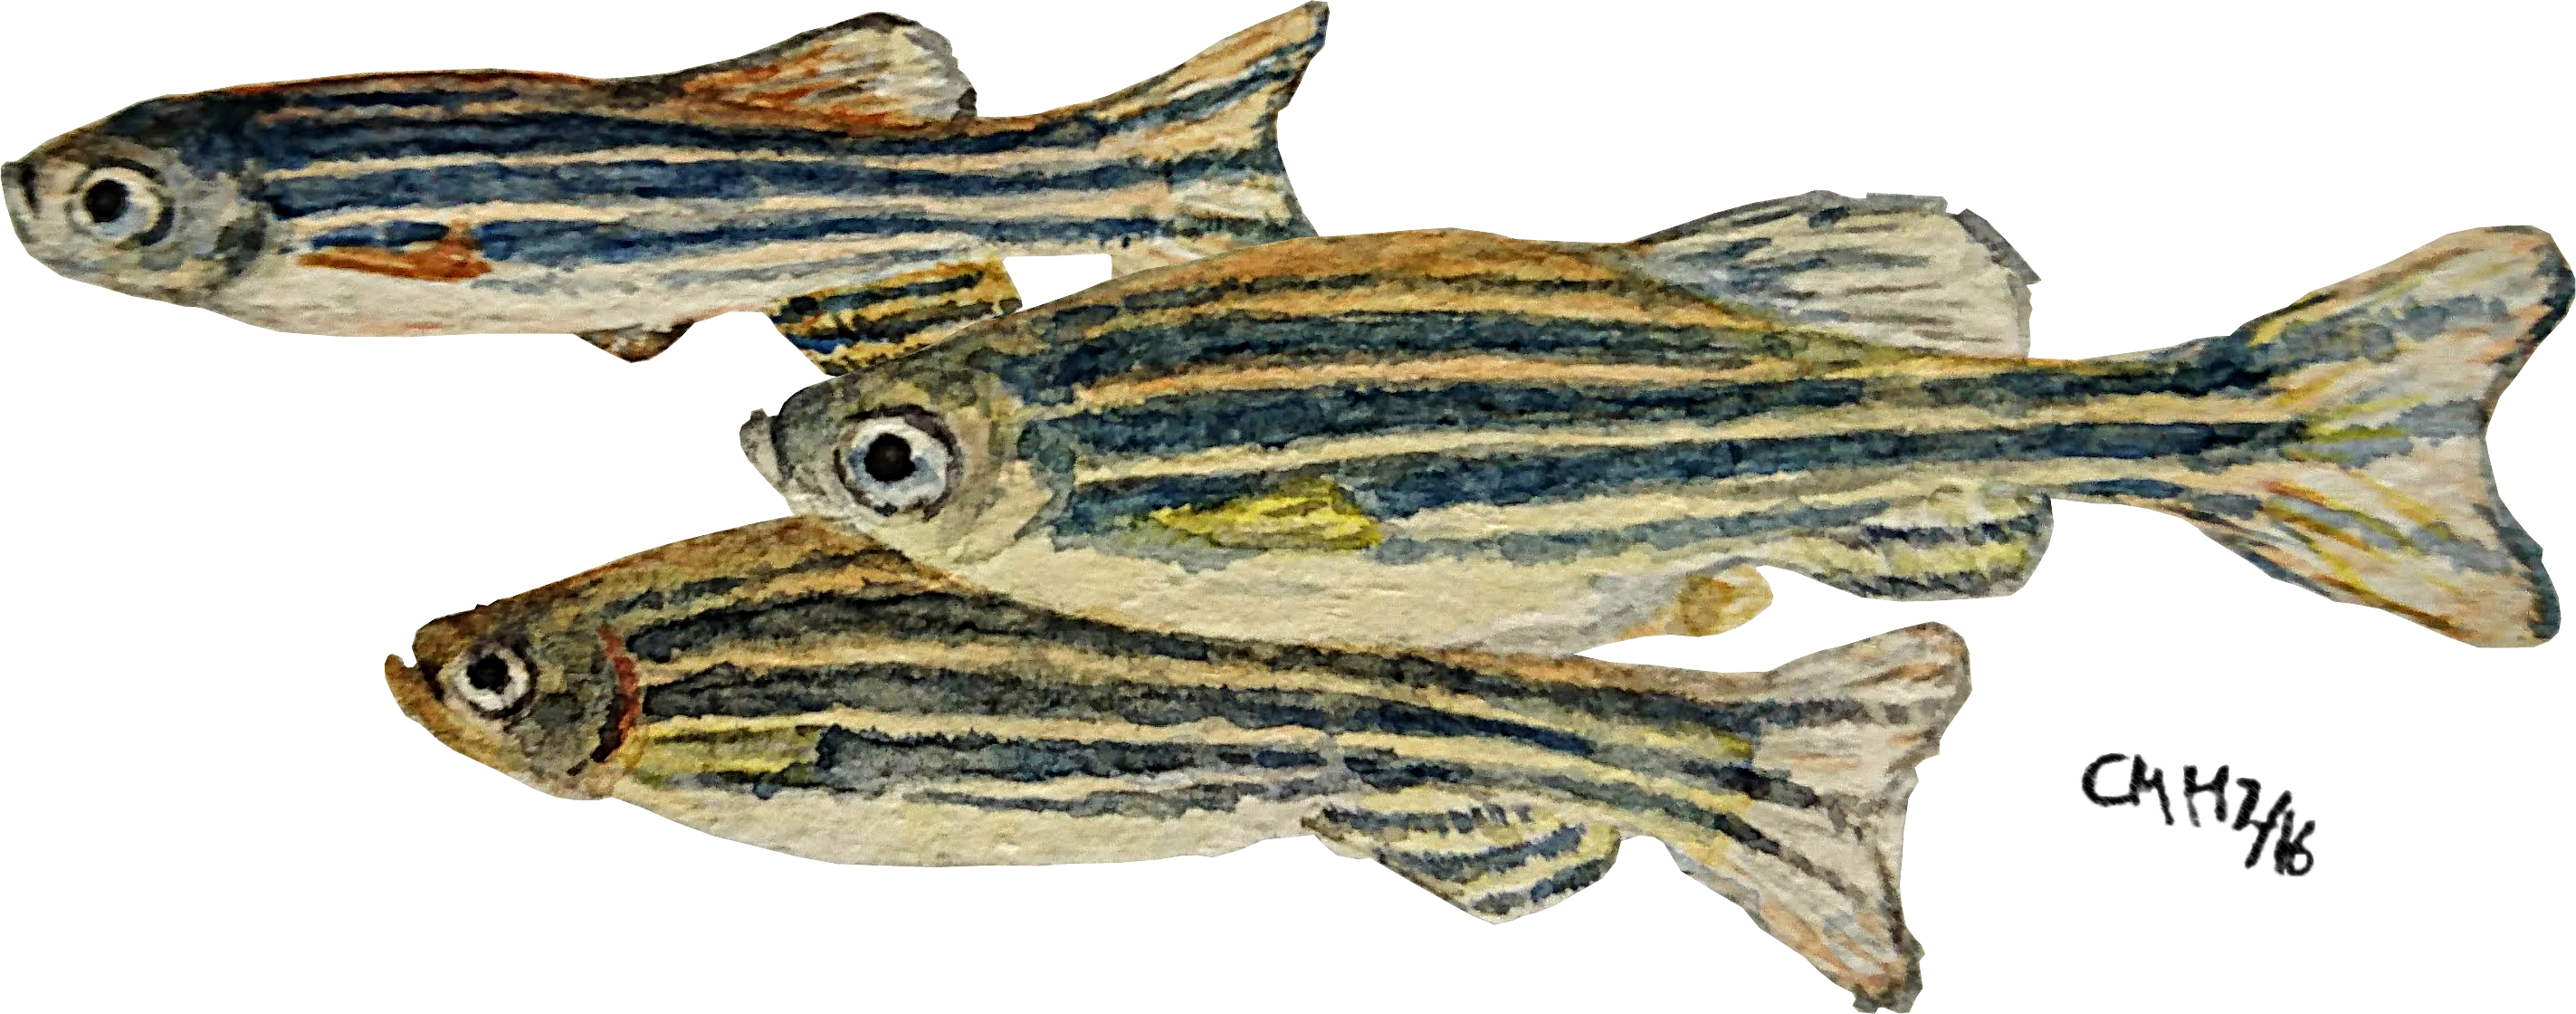
\includegraphics[width=0.50\textwidth]{figures/intro/CM_fish} 

}

\caption{Model organism \emph{Danio rerio} (aquarell by Christine Molenda)}\label{fig:zebra}
\end{figure}
\hypertarget{developmental-stages}{%
\subsection{Developmental Stages}\label{developmental-stages}}

A single female may lay up to 100 fertilized eggs. Each Zygote\footnote{first diploid cell after fertilization between two germ cells} then undergoes the first zygotic cell cycle (\textbf{up to 0.75 h}). The following two to seven cell cycles (period: \emph{Cleavage}, \textbf{up to 2.25 h}) occur directed and synchronous every \textasciitilde{}15 min. Cells in this stage are called \emph{blastomeres} and are incompletely undercut the \emph{blastodisc} (the collective of blastomeres) and remain interconnected by cytoplasmic bridges. The \emph{Blastula} period (up to 5.25 h) is determined by an increasing a-synchronicity between the cells, flattening of the blastodisc and lengthening of the cell cycle. This period is also marked by the onset of \emph{epiboly}\footnote{cells in late blastula start to dome, while a monolayer of the domes circumfence begins to wrap around the Yolk} (\emph{18}).

After Blastula and \textbf{up to 10 h} the \emph{Gastrula} period takes place, followed by the \emph{Segmentation} period (\textbf{up to 24 h}). Both of which are depicted in more detail in figure \ref{fig:stages}. At even later stages the embryo starts to elongate posteriorly, grow in size and develop organs until it first active muscle are present and it starts to swim (figure \ref{fig:stages}).


\begin{figure}

{\centering \includegraphics[width=.95\textwidth]{figures/intro/stages} 

}

\caption[Zebrafish embryonic development]{Zebrafish embryonic development. Microscopic images are from a time-lapse where 24 embryos were imaged simultaneously in brightfield and at 488 nm Z-Stacks. Representation shows contrast enhanced EDFs. Bottom row (30-48 hpf) stages are handmade drawings from live embryos made during the first week of my PhD.}\label{fig:stages}
\end{figure}
\hypertarget{the-lateral-line-system}{%
\subsection{The Lateral Line System}\label{the-lateral-line-system}}

The lateral line (LL) system is a mechano-sensory organ that is common to all teleost fish. It enables the animal to sense water movements and therefore to orient itself, and to detect prey and predators. Fully developed, the lateral line system is comprised of hundreds of neuromasts positioned in an orderly pattern all over the animal's body (figure \ref{fig:llsystem}A). Its functional subunits are the neuromasts (NM) (figure \ref{fig:llsystem}B-C) that, when fully developed, consist of hair-, support- and mantle cells. To sense water movements, each NM projects kinocilia out of the skin that, upon water induced deflection, create action potentials that are transduced via afferent and efferent fibers (\emph{19}, \emph{20}).


\begin{figure}

{\centering 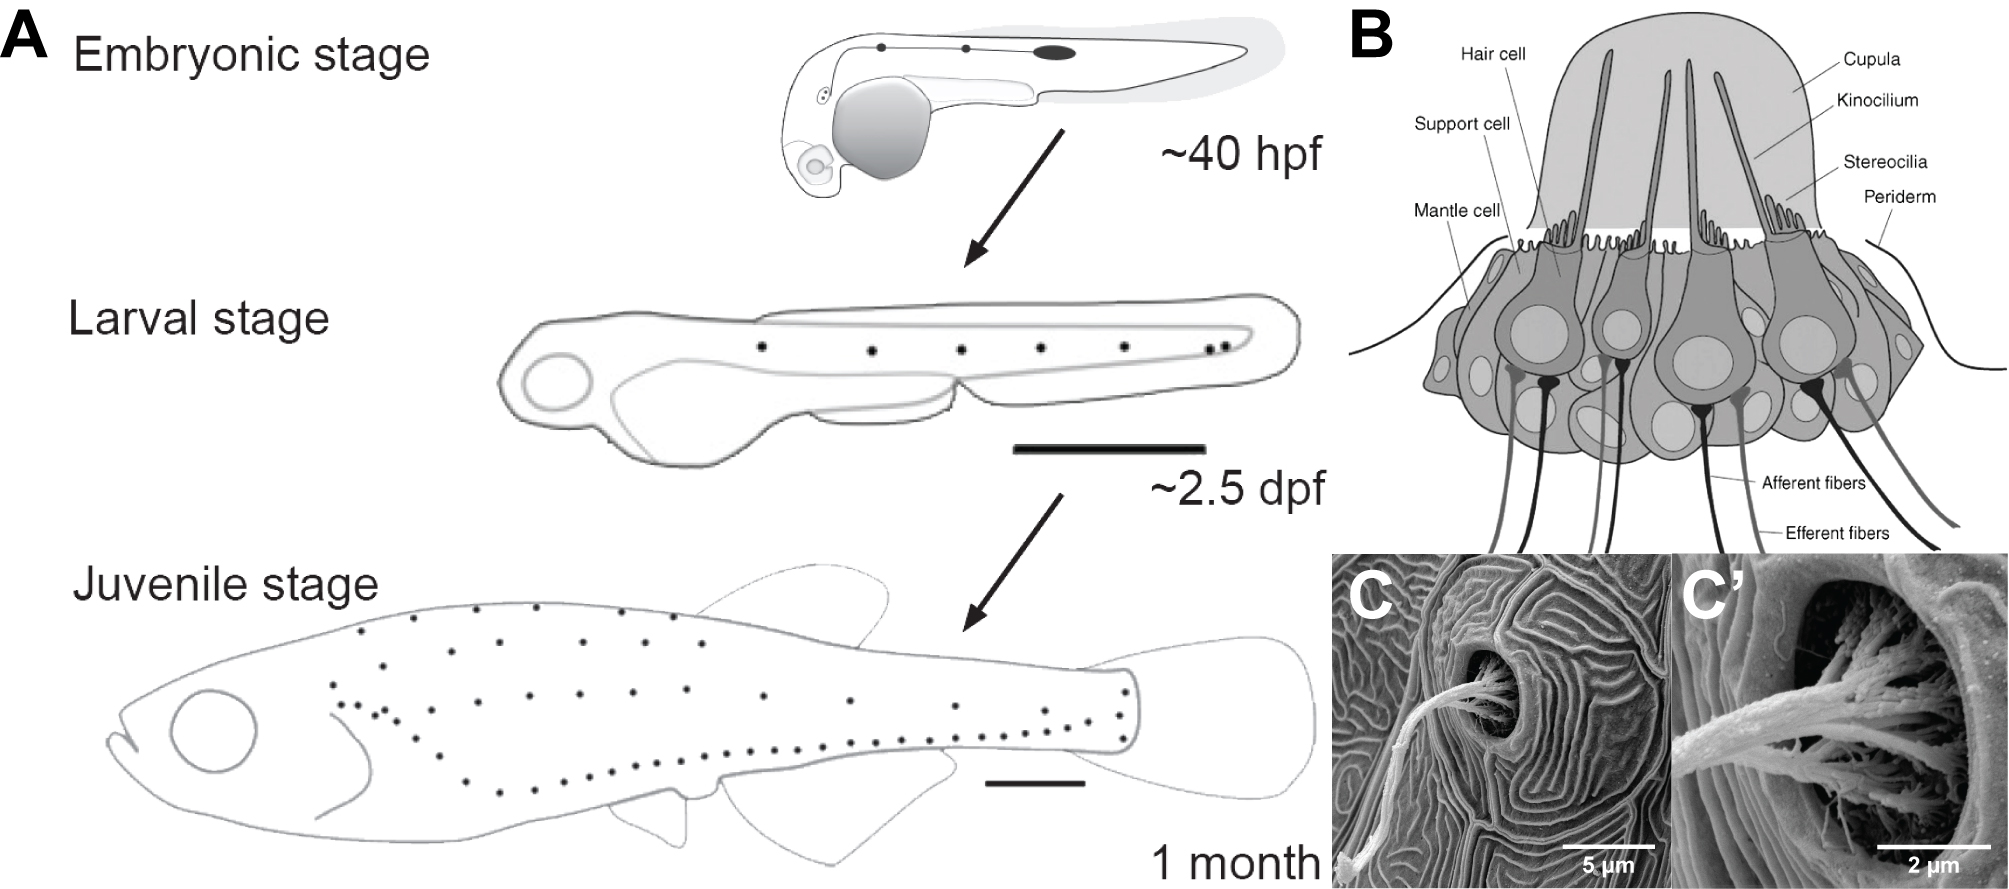
\includegraphics[width=.95\textwidth]{figures/intro/ll_system} 

}

\caption[The lateral line system]{The lateral line system. \textbf{A} modified after (Ghysen et al., 2012) and A.Bergs, 2016 (student presentation at AK Lecaudey). Development of the later line system at embryonic, larval and juvenile stage. \textbf{B} Schematic showing a crossection and organization of a single neuromast. \textbf{C-C'} SEM images of a single, pre-mature (3 dpf) neuromast.}\label{fig:llsystem}
\end{figure}
Each NM is first deposited as a premature cluster of about 30 cells from a migrating cell-aggregate called the posterior lateral line primordium (pLLP) \ref{fig:llgfp}A. The pLLP delaminates from the pLL placode, caudal to the otic vesicle (figure \ref{fig:llgfp}B) at around 20 \emph{hours post fertilization} (hpf) as a group of \textasciitilde{}100 cells. After formation of the leading region with cells undergoing EMT, it starts migrating along a chemokine gradient positioned at the horizontal myoseptum to the tip of the tail (figure \ref{fig:pllp}) (\emph{19}, \emph{20}). To ensure the development of a functional organ, several fundamental biological processes like cell migration, morphogenesis, proliferation and cell polarization need to be integrated into the pLLP.
An important breakthrough in LL research has been the development of a transgenic line expressing a membrane tethered GFP fusion protein (lyn-GFP) that is expressed under the LL specific promotor of \emph{cldnb} (claudin b\footnote{construct name: \emph{Tg(-8.0cldnb:lynGFP)}; ZFIN ID: ZDB-TGCONSTRCT-070117-15}) (\emph{21}), which allowed for a much more detailed view and to observe lateral line development \emph{in vivo}. An example of the fluorescence signal visible at \textasciitilde{}60 hpf can be seen in figure \ref{fig:llgfp}B.


\begin{figure}

{\centering 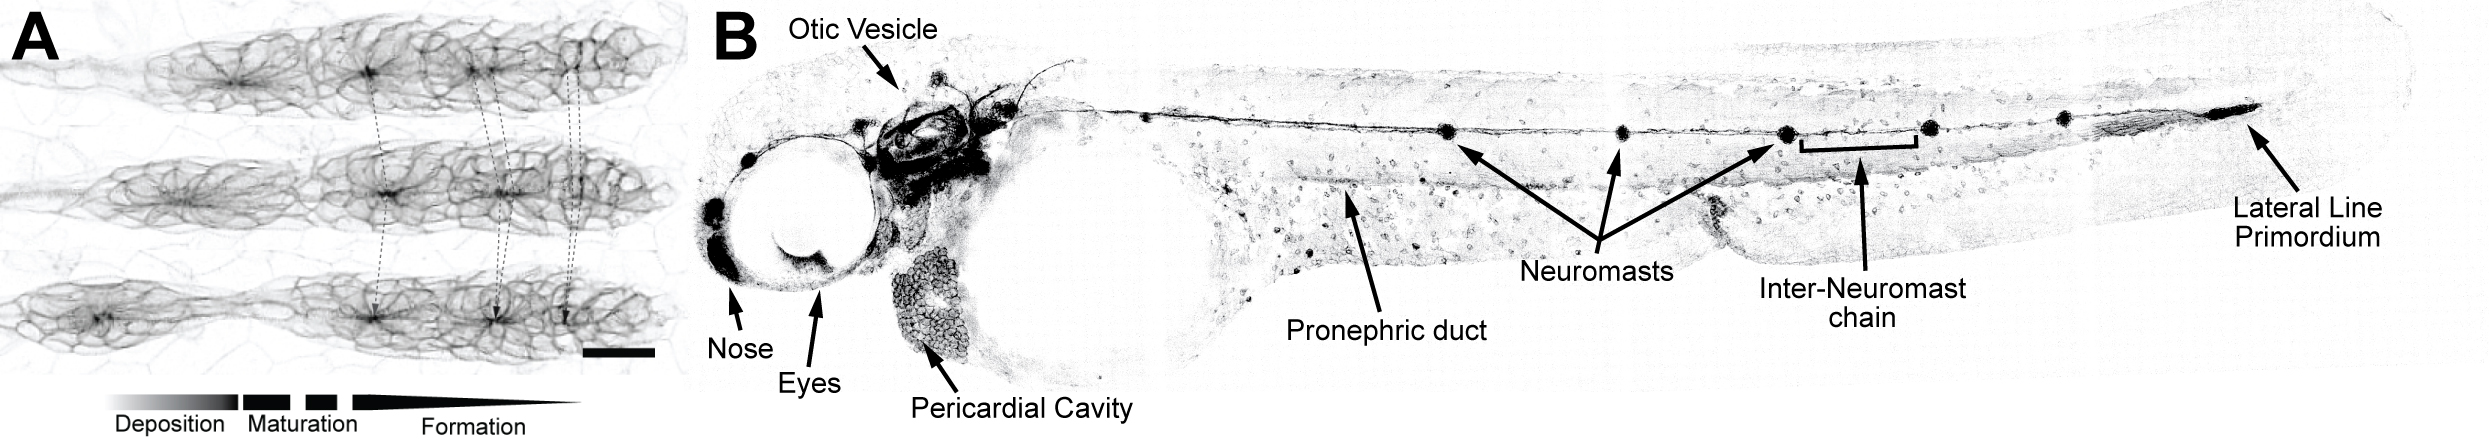
\includegraphics[width=.95\textwidth]{figures/intro/ll_gfp} 

}

\caption[Neuromast deposition and pattern]{Neuromast deposition and pattern \textbf{A} Scheme showing NM deposition over three timepoints (10 min. interval). Dotted lines are time-tracks of rosettes, which become more concentrated over time. Bottom arrow indicates regions of rosette formation, maturation and deposition within the pLLP (scale bar = 20 µm; 20X WI; \textasciitilde{}20 Z-planes; 2.5 µm spacing. MaxIP. Colors inverted.) \textbf{B} Scheme showing the lateral line at end of migration (\textasciitilde{}60 hpf) and other parts visible through the cldnb:lyn-gfp transgene (as documented through zfin.org) (air objective + 1.5X tube lens; four tiles; \textasciitilde{}20 Z-planes; 5 µm spacing. MaxIP. Colors inverted).}\label{fig:llgfp}
\end{figure}
\hypertarget{posterior-lateral-line-primordium}{%
\subsection{Posterior Lateral Line Primordium}\label{posterior-lateral-line-primordium}}

The pLLP is about 100-150 \(\mu\)m in length (depending on deposition cycle) over which it exhibits a diverse surface topology and cellular morphology. The current model assumes that the \emph{caudal} (also \emph{posterior}), more mesenchymal cells, are leading the path of migration, while the \emph{cranial} (also \emph{anterior}), more epithelial cells, are trailing. Towards the leading region the cells are more flat, towards the trailing region the cells become more columnar and increasingly radially organized into formations called epithelial rosettes (figure \ref{fig:pllp}). During migration the pLLP typically contains 2-3 \emph{rosettes} (\textasciitilde{}25-30 cells each), while the most trailing one will eventually be deposited to further mature to a functional NM (\emph{19}, \emph{22}). Since every deposition comes with a loss of cells in the pLLP, cells need to be regenerated. While one study concludes a spatial heterogeneity in distribution of proliferative cells (\emph{23}), another one suggests a higher proliferative rate near the leading region (\emph{24}).


\begin{figure}

{\centering 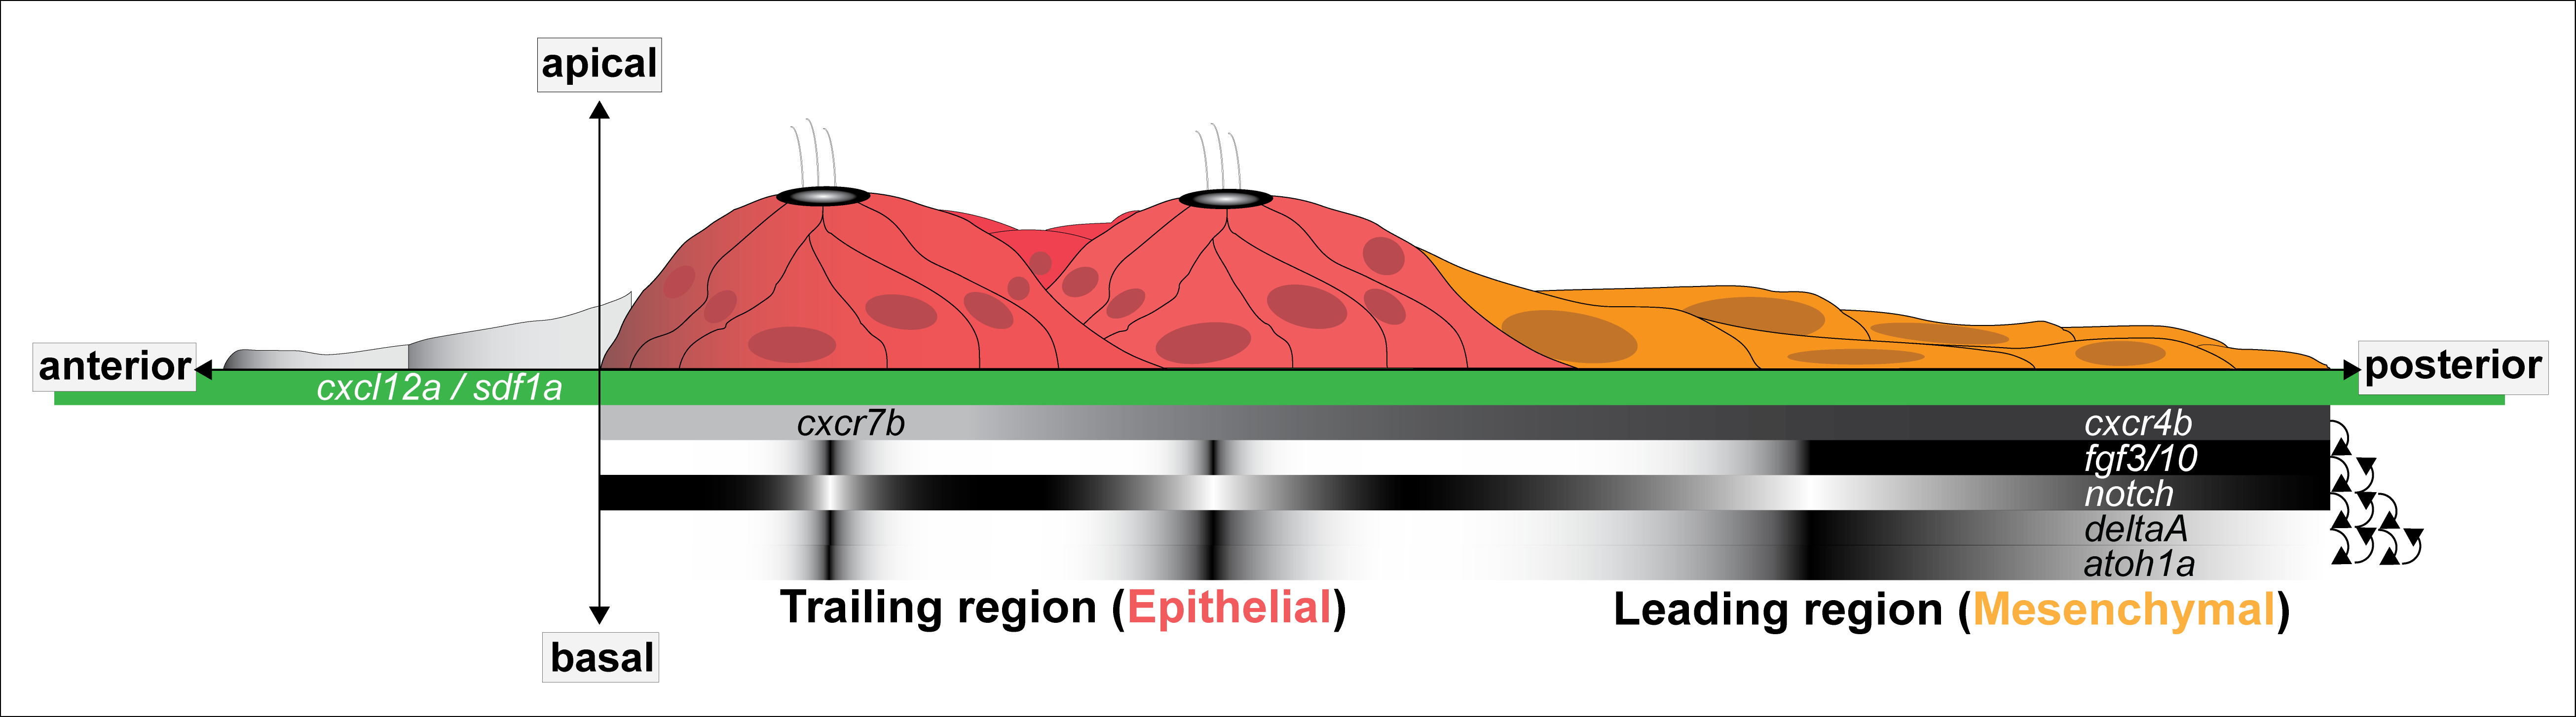
\includegraphics[width=.75\textwidth]{figures/intro/pllp} 

}

\caption[Summary of signaling gradients within the pLLP]{Summary of signaling gradients within the pLLP. Cross-section of the lateral line primordium. (red = trailing region, yellow = leading region; embryonic axes indicated by arrows. Signaling gradients indicated by black-white gradients, sorted by hierarchy.)}\label{fig:pllp}
\end{figure}
\hypertarget{rosette-formation}{%
\subsubsection{Rosette formation}\label{rosette-formation}}

The onset of morphological and functional changes is determined by signaling of Fgf, which is mostly active in the trailing region. Causal for expression of Fgf is a signaling center of WNT in the leading region, which promotes expression of Fgf ligands \emph{Fgf-3} and \emph{-10} (\emph{25}). Those ligands then diffuse to the trailing domain where binding through \emph{Fgf receptor 1} (Fgfr1) triggers a signaling cascade through which the cells become more columnar, apically constricted and eventually re-organize into epithelial rosettes (\emph{24}, \emph{26}, \emph{27}). Concurrently, cells of the Wnt signaling center themselves are not competent to Fgf signaling, which is achieved through expression of \emph{Sef}, an intracellular antagonist to Fgfr1 signaling (\emph{28}). In a more recent publication (\emph{29}) it was shown that Shroom3 plays a key role in mediating AC and rosette formation in the pLLP.

\hypertarget{hair-cell-specification}{%
\subsubsection{Hair cell specification}\label{hair-cell-specification}}

Downstream of Fgf lies the expression of transcription factor (TF) atoh1a, which gives cells the potential to become sensory hair cells (\emph{24}). The current model suggests that Fgf initiates expression of \emph{atoh1a} and \emph{deltaA}, where DeltaA activates Notch in neighboring cells to inhibit expression of \emph{atoh1a} in those. Atoh1a in turn suppresses competence for Fgf and initiates expression of \emph{atoh1b} and \emph{deltaD}. While the latter acts synergistic with DeltaA, Atoh1b again drives expression of \emph{atoh1a} (\emph{30}). Once a prospective hair cell is specified it will itself become a source for Fgf-10. By this process adjacent cells are laterally inhibited and determined \emph{support cells} (figure \ref{fig:llsystem}B), still capable of receiving Fgf signals.

Just before the most trailing rosette is deposited, its prospective hair cell will undergo a final division to form a doublet of sensory hair cells that will orient orthogonal to planar polarity and establish mirror symmetry in maturing neuromasts (\emph{31}, \emph{32}).

\hypertarget{shroom3-in-the-pllp}{%
\subsection{Shroom3 in the pLLP}\label{shroom3-in-the-pllp}}

The Shroom protein family is conserved through evolution (supplementary figure) and involved in contraction of the actomyosin network (e.g.~during AC), which has been confirmed in several studies \emph{e.g.} investigating e.g.~epithelial planar remodelling, neural tube morphogenesis, \emph{Xenopus} bottle cells and epithelial invagination (\emph{33}--\emph{38}). Furthermore, Shroom might be a novel candidate involved in heterotaxy (\emph{39}).

\hypertarget{intro-shroom}{%
\subsubsection{Recent research}\label{intro-shroom}}

Shroom proteins have three characteristic domains (1) a \emph{PDZ} domain close to the N-terminus to interact with other proteins with PDZ domains and (2) two \emph{Apx/Shroom} domains (ASD1 and 2), the latter being close to the proteins C-terminus. The Shroom domains may interact with proteins containing a \emph{Shroom binding domain} (SBD) such as Rock to help and facilitate phosphorylation of NMII (figure \ref{fig:shrminteract}) (\emph{40}).


\begin{figure}

{\centering 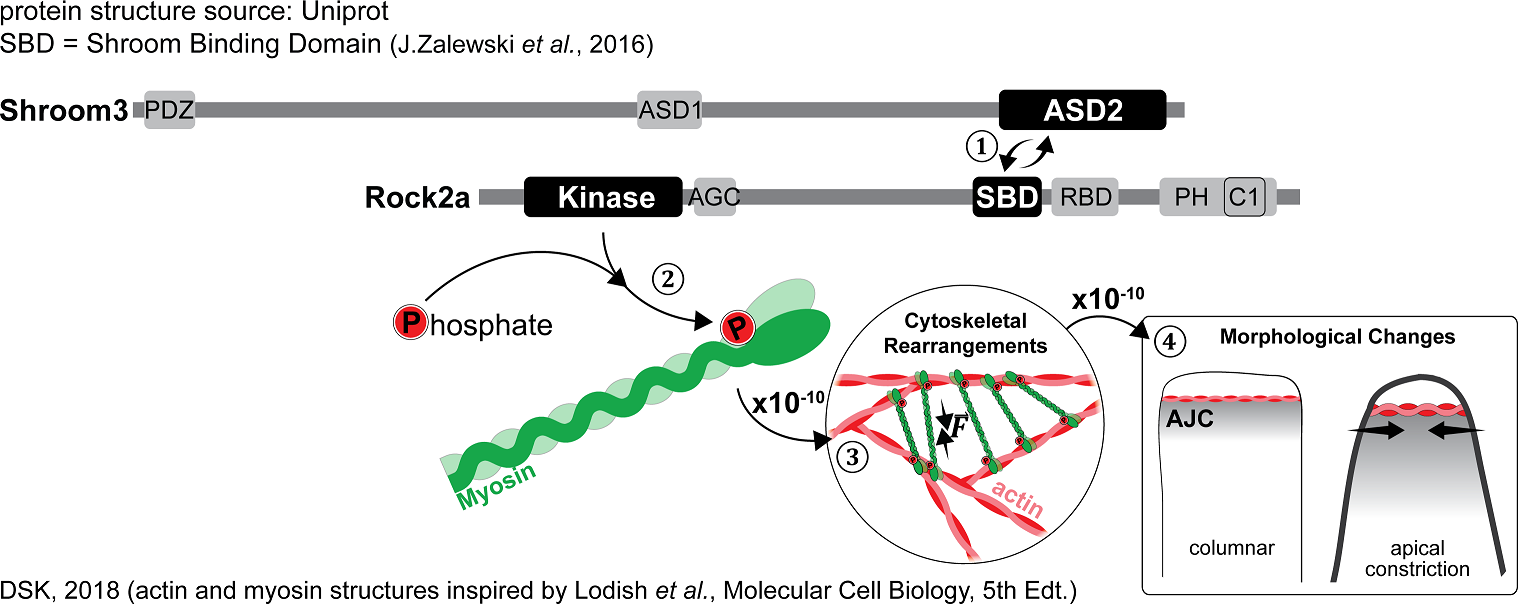
\includegraphics[width=.95\textwidth]{figures/intro/shrm3_interaction} 

}

\caption[Shroom3 functional domains and mode of operation]{Shroom3 functional domains and mode of operation. Sequence of events numbered from 1-4. Approximate scale jumps indicated at arrows.}\label{fig:shrminteract}
\end{figure}
While in all of the above-mentioned studies Shroom3 was the focus of interest, in zebrafish and most other model organisms there are four paralogs. A previous study done on Shroom3 morphants in \emph{D.rerio} (\emph{29}) indicates that Shroom3 is also necessary for AC and rosette formation in the migrating pLLP. In summary they were able to show and that
\begin{enumerate}
\def\labelenumi{\arabic{enumi}.}
\tightlist
\item
  Shroom3 is indeed expressed in the pLLP from stages 24 -- 48 hpf which was confirmed via \emph{in situ} hybridization (ISH)
\item
  \emph{shroom3} is expressed downstream of Fgf signalling, which was confirmed via treatment with an Fgfr1 inhibiting drug. Subsequent ISH with the Probe used before showed that the signal was gone in Morpholino (MO) injected embryos. The drug used has been used before (SU5402) in the same context (\emph{24}, \emph{27}). In these it was found that SU5402 has the ability to prevent rosette formation, but not to dismantle already established ones.
\item
  Shroom3 localizes to rosette centers, which was accomplished by inserting a genetic construct where a \emph{shroom3-tagRFP} fusion protein is under control of a heat-shock\footnote{heat shock proteins are \emph{Escherichia coli} enzymes that assist protein folding and are heat activated} promotor into a \emph{cldnb:lyn-GFP} transgenic line. This way they were able to ectopically express \emph{shroom3-tRFP} and confirm its localization by confocal fluorescence microscopy (figure \ref{fig:shrmernst}A).
\item
  Rosette formation is impaired, which was confirmed quantitatively by using a specifically trained \emph{rosette detector} (\emph{41}) to count and weight single rosettes. As a metric to compare whole pLLPs the sum of weights as in \(\sum_{i=1}^{i-n}{weighted\ detections}\) was used (figure \ref{fig:shrmernst}B-B').
\end{enumerate}

\begin{figure}

{\centering 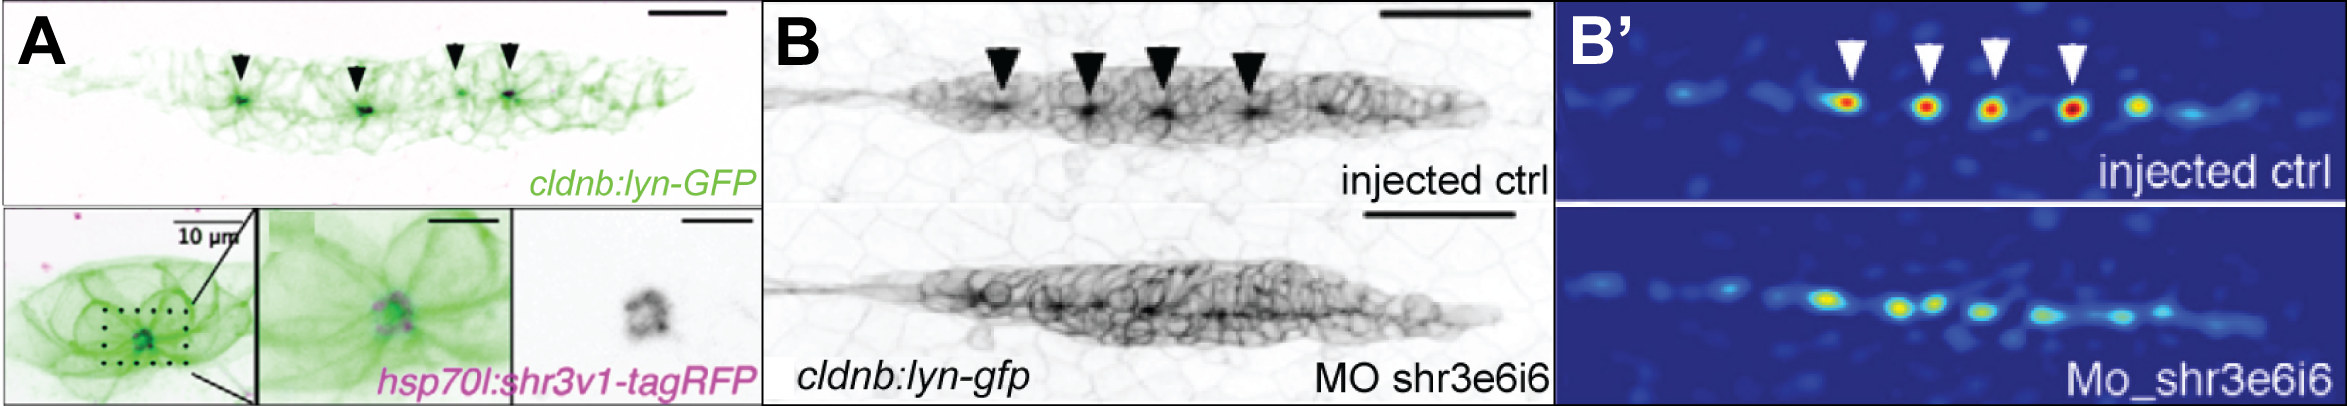
\includegraphics[width=.95\textwidth]{figures/intro/shrm_ernst} 

}

\caption[Shroom3 in rosette formation]{Shroom3 in rosette formation (adapted from Ernst et al., 2012) \textbf{A} composite MaxIPs of membrane label and fusion protein showing the localization of Shroom within the pLLP \textbf{B} uninjected control and shroom3 MO injected MaxIPs \textbf{B'} Heat-maps of rosette detector score.}\label{fig:shrmernst}
\end{figure}
\hypertarget{current-model}{%
\subsubsection{Current Model}\label{current-model}}

Based on these and previous results, the current model for apical constriction in the pLLP assumes that (1) expression of \emph{shroom3} is induced by Fgf signaling (2) Shroom3 binds Rock and translocates to the AJC to (3) mediate phosphorylation of NMII which (3) induces contraction of the actin network and AC (figure \ref{fig:shrmmodel}). Furthermore, AC is necessary for rosette assembly and subsequent NM deposition. In conclusion the current understanding is that without Shroom3 AC can not take place and rosette formation does not occur, therefore NMs are not deposited.


\begin{figure}

{\centering 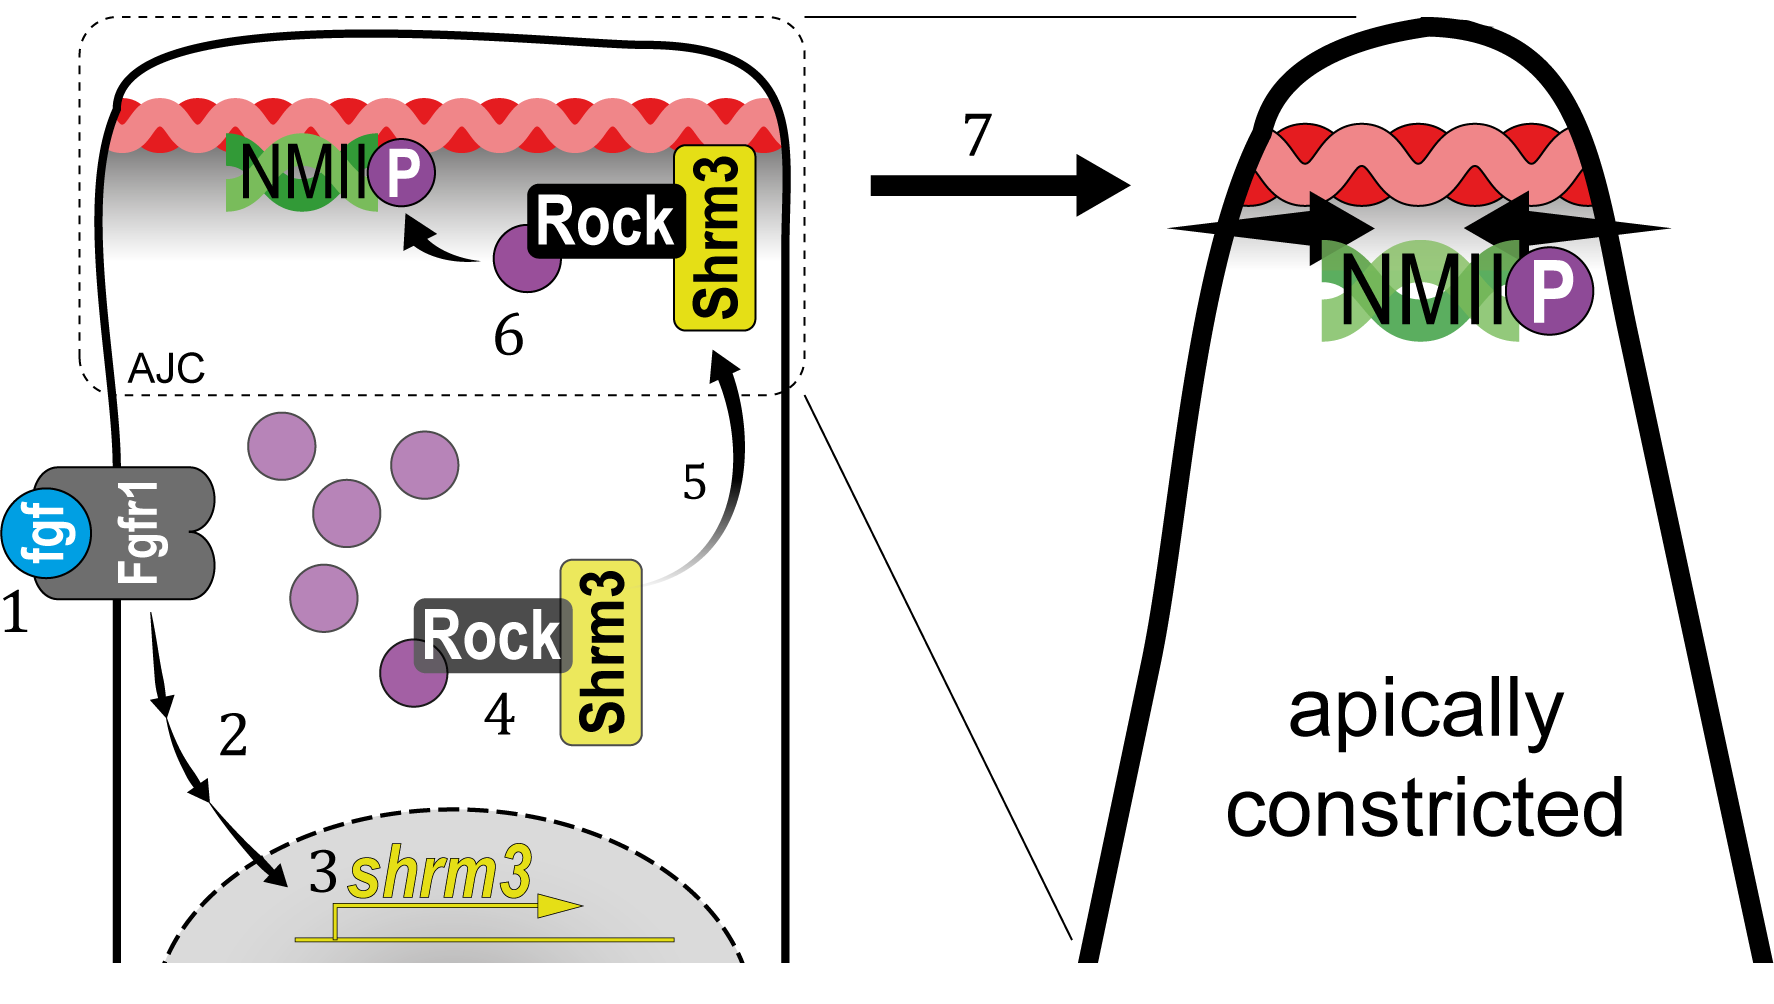
\includegraphics[width=.70\textwidth]{figures/intro/shrm_model} 

}

\caption{Shroom3 current model}\label{fig:shrmmodel}
\end{figure}
\hypertarget{shroom3-mutants}{%
\subsection{\texorpdfstring{\emph{shroom3} mutants}{shroom3 mutants}}\label{shroom3-mutants}}

The strategy for the mutant was to inhibit interaction with SBD-domain proteins. Furthermore, the mutant should be easily genotyped by amplifying a fragment of the gene via PCR and correlating gel electrophoresis band patterns after a restrictive digest. To achieve this, an eight base pair deletion was introduced in Shroom domain 1 (SD1) using the \emph{Transcription activator-like effector nuclease} (TALEN) (\emph{42}) genome editing system that would prevent interaction with SBD-domain proteins, or even lead to a NULL mutation\footnote{mutation that leads to a complete loss of function} (figure \ref{fig:shrmmut}A-A'). The mutation lead to (1) a shift in the open reading frame and to a pre-mature stop codon and (2) a deletion of a restriction site for a restriction enzyme named NsiI (figure \ref{fig:shrmmut}B-B').

\hypertarget{intro-phen}{%
\subsubsection{Phenotype description}\label{intro-phen}}

While birth rates follow a distribution of Mendelian inheritance (after genotyping at 3 months of age), mutant adults are more sensitive to mechanical stress and have a shortened lifespan (\textasciitilde{}6-9 months). In body shape, \emph{shroom3} mutants are not smaller or posses any other striking phenotype (figure \ref{fig:shrmmut}C), however their gill flaps seem to be increased in size, swollen, and not exactly streamlined with the body. This is also evident by an increased frequency of gill flap beating. When looking at the pLLP at different stages (figure \ref{fig:shrmmut}D), they exhibit the same phenotype as the MO injected embryos. Here it is noteworthy that a fraction of about 20\(\%\) of the pLLPs exhibit a more wildtype (or \emph{weak}) phenotype, even though these embryos were genotyped as homozygous\footnote{when both alleles are the same} mutant. A possible reason for this will also be subject of thesis. Figure \ref{fig:shrmmut}E shows exemplary specimen at about 60 hpf where for the mutant, the first thing that catches the eye is the increase in the number of clusters\footnote{forth on Neuromasts will be called `cell clusters} deposited. Interestingly, this is rather contradictive to the current model of Shroom3's function during LL development.


\begin{figure}

{\centering \includegraphics[width=.95\textwidth]{figures/intro/shrm_mutants} 

}

\caption[shroom3 mutant phenotype]{\emph{shroom3} mutant phenotype \textbf{(A-A')} mutation strategy (A) Talen arms (black blocks) bordering a sequence within SD1 including a restriction site for NsiI (indicated back arrows and grey background) (A') wildtype and mutant allele with 8 bp deletion \textbf{(B-B')} Amino acid code and protein schematic with functional domains and stop codon (indicated by asterisk) \textbf{(C-C')} Adult phenotype with closeup to gill flaps \textbf{(D)} pLLP phenotype for three different stages (columns) and different manifestations (rows) (40X WI objective). Arrows indicate epithelial rosettes. \textbf{(E)} LL phenotype at end of migration (10X air objective). Scale bars = 1 mm. MaxIPs for D-E.}\label{fig:shrmmut}
\end{figure}
\hypertarget{objective-and-open-questions}{%
\section{Objective and Open Questions}\label{objective-and-open-questions}}

After having the results of the morpholino induced phenotype, a mutant was generated whose pLLP phenotype closely resembled the morpholino induced one. However, the phenotype at later stages revealed discrepancies with the current model and the role of Shroom3 during LL development.

\hypertarget{motivation}{%
\subsection{Motivation}\label{motivation}}

Due to the pLLP's relative simplicity (\textasciitilde{}100 cells), excellent accessibility for advanced light-microscopes (\textasciitilde{}1 cell layer beneath the skin) and a broad and well-established palette of available methods, it promises an \emph{in toto} understanding and complete model of factors leading to its development. Having access to such a model may be very beneficial to other fields such as organ regeneration, cancer- and clinical research.

In this scenario, the advantages of working with a knockout- as compared to a knockdown\footnote{permanent versus transient mutation} mutant are (1) an equal amount of gene expression across all samples (2) no side effects due to injection procedure or solvents in drug treatments (3) the ability to observe the effects of the mutation for very long periods of time.

One aspect about LL development that still remains unclear are the exact factors that lead to cell cluster (CC) deposition. What determines the timing of deposition? When is a rosette mature enough to be deposited? What happens to the cells before and after deposition? How do the cells specify before deposition? What are the morphological features of depositing cells? What influence does morphology have on Neuromast deposition?

Using the Shroom3 mutants as a model system offers great potential to shed new light on organogenesis, the interplay between morphogenesis and cellular specification, epithelial rosette formation and neuromast deposition.

\hypertarget{data-strategy-and-analysis}{%
\section{Data Strategy and Analysis}\label{data-strategy-and-analysis}}

Due to the history of Developmental Biology and the complexity of biological processes \emph{per se}, the field heavily relies on image data. Since the advent of electronic imaging techniques\footnote{e.g.~photomultipliers or charge-coupled devices} scientific image data can be processed and analyzed \emph{in silico}. To make use of the possibility of
\begin{enumerate}
\def\labelenumi{\arabic{enumi}.}
\tightlist
\item
  live imaging, which (as compared to fixation techniques) conserves the cellular integrity and morphology while also offers the possibility of recording time-lapses
\item
  the optically clear specimen and
\item
  high throughput image analysis and state-of-the-art data science using algorithmic implementations,
\end{enumerate}
the three following points were paid special attention to.

\hypertarget{sample-preparation}{%
\subsection{Sample Preparation}\label{sample-preparation}}

For fluorescence microscopy zebrafish embryos are usually immersed in a 1\% solution of \emph{low melting-point agarose} (LMPA) solution and then oriented on an optical cover slip manually until the LMPA has solidified. This process allows to mount\footnote{the process of embedding the samples in agarose} eight to ten embryos \emph{per} dish. To make use of the high number of offspring a single zebrafish female may lay, which rapidly leads to a sample number of more than 300, a new sample preparation technique was devised that allows for (1) a four to five times increase in samples per dish (2) a facilitated navigation \emph{via} a grid-like orientation through the samples and (3) an improved spatial orientation where the embryos body axes are aligned parallel to the optical Z-sections of the confocal microscope. For details, see Materials and Methods section \ref{mount-met} and Kleinhans \emph{et al.}, 2019.

\hypertarget{imaging}{%
\subsection{Imaging}\label{imaging}}

Technically, speed and sensitivity are most important for live imaging. Considering these two parameters a light-sheet (\emph{43}) fluorescence microscope (LSFM) would be the best fit. However, LSFMs also have several limitations. First, due to the sample preparation methods available the number of samples that can be imaged at a time is highly restricted. Second, for subcellular resolution a high magnification is required, which is limited by working distances and third - for optimal image analysis a high Signal-to-Noise ratio (SNR) and numerical aperture (N.A.) is preferable. Therefore a spinning disc (\emph{44}) system was chosen for most of the imaging.
The system makes use of (1) an extra-large field of view (FOV) ideal for large specimen (2) the possibility of a high degree of automation with state-of-the-art software and (3) a water dispension system for long-term water immersion imaging. For details about the system see Materials and Methods section \ref{mat-SD}.

\hypertarget{data-handling}{%
\subsection{Data handling}\label{data-handling}}

Subsequently after data acquisition and pre-processing the image data was transferred from the microscope system to the labs main workstation. To uniquely identify each file and have them appear in a structured manner, a file-naming system was established after the following structure

\makebox[\linewidth]{$[stage]\_[group]\_[id]\_[date]$}
\newline

Where \emph{stage} would e.g.~be 32hpf, \emph{group} would be a genotype or drug treatment, \emph{id} would be a positional identifier on an imaging dish like B1P01\footnote{Where B stands for a batch, that is if multiple dishes were imaged and P stands for the position within a single batch} and \emph{date} would be a date in the form of YYMMDD.

\hypertarget{image-and-data-analysis}{%
\subsection{Image and Data Analysis}\label{image-and-data-analysis}}

In order to be as objective an as high throughput as possible, almost all of the analyses performed for this study was solved using either algorithmically or state-of-the-art convolutional neural networks (CNNs). Furthermore, to meet the terms and conditions of \emph{open science}\footnote{``movement to make scientific research {[}\ldots{}{]} and its dissemination accessible to all levels of an inquiring society'' -- Wikipedia/en/Open\_science} standards, all pipelines were implemented in open source software frameworks such as \emph{Fiji is just image J} (FIJI) and R. For further information about training datasets, algorithms and versions used see Materials and Methods section \ref{mat-sftwr}.

\hypertarget{mat-met}{%
\chapter{Materials and Methods}\label{mat-met}}

\hypertarget{mat}{%
\section{Materials}\label{mat}}

\hypertarget{mat-chem}{%
\subsection{Chemicals}\label{mat-chem}}
\begin{longtable}[]{@{}rcl@{}}
\caption{\label{tab:mat-chem} Chemicals}\tabularnewline
\toprule
\begin{minipage}[b]{0.26\columnwidth}\raggedleft
\textbf{Chemical}\strut
\end{minipage} & \begin{minipage}[b]{0.50\columnwidth}\centering
Company\strut
\end{minipage} & \begin{minipage}[b]{0.16\columnwidth}\raggedright
cat.-no.\strut
\end{minipage}\tabularnewline
\midrule
\endfirsthead
\toprule
\begin{minipage}[b]{0.26\columnwidth}\raggedleft
\textbf{Chemical}\strut
\end{minipage} & \begin{minipage}[b]{0.50\columnwidth}\centering
Company\strut
\end{minipage} & \begin{minipage}[b]{0.16\columnwidth}\raggedright
cat.-no.\strut
\end{minipage}\tabularnewline
\midrule
\endhead
\begin{minipage}[t]{0.26\columnwidth}\raggedleft
Agarose\strut
\end{minipage} & \begin{minipage}[t]{0.50\columnwidth}\centering
Roth\strut
\end{minipage} & \begin{minipage}[t]{0.16\columnwidth}\raggedright
6351.2\strut
\end{minipage}\tabularnewline
\begin{minipage}[t]{0.26\columnwidth}\raggedleft
Agar-Agar\strut
\end{minipage} & \begin{minipage}[t]{0.50\columnwidth}\centering
Roth\strut
\end{minipage} & \begin{minipage}[t]{0.16\columnwidth}\raggedright
5210.3\strut
\end{minipage}\tabularnewline
\begin{minipage}[t]{0.26\columnwidth}\raggedleft
Ampicillin\strut
\end{minipage} & \begin{minipage}[t]{0.50\columnwidth}\centering
Roth\strut
\end{minipage} & \begin{minipage}[t]{0.16\columnwidth}\raggedright
K029.2\strut
\end{minipage}\tabularnewline
\begin{minipage}[t]{0.26\columnwidth}\raggedleft
ATP\strut
\end{minipage} & \begin{minipage}[t]{0.50\columnwidth}\centering
Epicentre\strut
\end{minipage} & \begin{minipage}[t]{0.16\columnwidth}\raggedright
E311K\strut
\end{minipage}\tabularnewline
\begin{minipage}[t]{0.26\columnwidth}\raggedleft
Blocking Reagent\strut
\end{minipage} & \begin{minipage}[t]{0.50\columnwidth}\centering
Roche\strut
\end{minipage} & \begin{minipage}[t]{0.16\columnwidth}\raggedright
11096176001\strut
\end{minipage}\tabularnewline
\begin{minipage}[t]{0.26\columnwidth}\raggedleft
BCIP\strut
\end{minipage} & \begin{minipage}[t]{0.50\columnwidth}\centering
Fermentas\strut
\end{minipage} & \begin{minipage}[t]{0.16\columnwidth}\raggedright
R0822\strut
\end{minipage}\tabularnewline
\begin{minipage}[t]{0.26\columnwidth}\raggedleft
CaCl\textsubscript{2}\strut
\end{minipage} & \begin{minipage}[t]{0.50\columnwidth}\centering
Roth\strut
\end{minipage} & \begin{minipage}[t]{0.16\columnwidth}\raggedright
886.1\strut
\end{minipage}\tabularnewline
\begin{minipage}[t]{0.26\columnwidth}\raggedleft
Calyculin\strut
\end{minipage} & \begin{minipage}[t]{0.50\columnwidth}\centering
\strut
\end{minipage} & \begin{minipage}[t]{0.16\columnwidth}\raggedright
\strut
\end{minipage}\tabularnewline
\begin{minipage}[t]{0.26\columnwidth}\raggedleft
DIG RNA Mix\strut
\end{minipage} & \begin{minipage}[t]{0.50\columnwidth}\centering
Roche\strut
\end{minipage} & \begin{minipage}[t]{0.16\columnwidth}\raggedright
11277073910\strut
\end{minipage}\tabularnewline
\begin{minipage}[t]{0.26\columnwidth}\raggedleft
DMSO\strut
\end{minipage} & \begin{minipage}[t]{0.50\columnwidth}\centering
Roth\strut
\end{minipage} & \begin{minipage}[t]{0.16\columnwidth}\raggedright
4720.2\strut
\end{minipage}\tabularnewline
\begin{minipage}[t]{0.26\columnwidth}\raggedleft
EtBr\strut
\end{minipage} & \begin{minipage}[t]{0.50\columnwidth}\centering
Roth\strut
\end{minipage} & \begin{minipage}[t]{0.16\columnwidth}\raggedright
2218.3\strut
\end{minipage}\tabularnewline
\begin{minipage}[t]{0.26\columnwidth}\raggedleft
EtOH\strut
\end{minipage} & \begin{minipage}[t]{0.50\columnwidth}\centering
Roth\strut
\end{minipage} & \begin{minipage}[t]{0.16\columnwidth}\raggedright
9065.3\strut
\end{minipage}\tabularnewline
\begin{minipage}[t]{0.26\columnwidth}\raggedleft
Formaldehyde\strut
\end{minipage} & \begin{minipage}[t]{0.50\columnwidth}\centering
Roth\strut
\end{minipage} & \begin{minipage}[t]{0.16\columnwidth}\raggedright
7398.1\strut
\end{minipage}\tabularnewline
\begin{minipage}[t]{0.26\columnwidth}\raggedleft
Formamide\strut
\end{minipage} & \begin{minipage}[t]{0.50\columnwidth}\centering
Roth\strut
\end{minipage} & \begin{minipage}[t]{0.16\columnwidth}\raggedright
P040.1\strut
\end{minipage}\tabularnewline
\begin{minipage}[t]{0.26\columnwidth}\raggedleft
Glycerol\strut
\end{minipage} & \begin{minipage}[t]{0.50\columnwidth}\centering
Roth\strut
\end{minipage} & \begin{minipage}[t]{0.16\columnwidth}\raggedright
3783.2\strut
\end{minipage}\tabularnewline
\begin{minipage}[t]{0.26\columnwidth}\raggedleft
IPTG\strut
\end{minipage} & \begin{minipage}[t]{0.50\columnwidth}\centering
Thermo\strut
\end{minipage} & \begin{minipage}[t]{0.16\columnwidth}\raggedright
R1171\strut
\end{minipage}\tabularnewline
\begin{minipage}[t]{0.26\columnwidth}\raggedleft
KCl\strut
\end{minipage} & \begin{minipage}[t]{0.50\columnwidth}\centering
Roth\strut
\end{minipage} & \begin{minipage}[t]{0.16\columnwidth}\raggedright
P017.1\strut
\end{minipage}\tabularnewline
\begin{minipage}[t]{0.26\columnwidth}\raggedleft
Low melting point Agarose\strut
\end{minipage} & \begin{minipage}[t]{0.50\columnwidth}\centering
Roth\strut
\end{minipage} & \begin{minipage}[t]{0.16\columnwidth}\raggedright
A9539\strut
\end{minipage}\tabularnewline
\begin{minipage}[t]{0.26\columnwidth}\raggedleft
Maleic Acid\strut
\end{minipage} & \begin{minipage}[t]{0.50\columnwidth}\centering
\strut
\end{minipage} & \begin{minipage}[t]{0.16\columnwidth}\raggedright
\strut
\end{minipage}\tabularnewline
\begin{minipage}[t]{0.26\columnwidth}\raggedleft
MeOH\strut
\end{minipage} & \begin{minipage}[t]{0.50\columnwidth}\centering
Roth\strut
\end{minipage} & \begin{minipage}[t]{0.16\columnwidth}\raggedright
CP43.3\strut
\end{minipage}\tabularnewline
\begin{minipage}[t]{0.26\columnwidth}\raggedleft
MgCl\textsubscript{2}\strut
\end{minipage} & \begin{minipage}[t]{0.50\columnwidth}\centering
Roth\strut
\end{minipage} & \begin{minipage}[t]{0.16\columnwidth}\raggedright
2189.1\strut
\end{minipage}\tabularnewline
\begin{minipage}[t]{0.26\columnwidth}\raggedleft
NaCl\strut
\end{minipage} & \begin{minipage}[t]{0.50\columnwidth}\centering
Roth\strut
\end{minipage} & \begin{minipage}[t]{0.16\columnwidth}\raggedright
9265.2\strut
\end{minipage}\tabularnewline
\begin{minipage}[t]{0.26\columnwidth}\raggedleft
NaHCO\textsubscript{3}\strut
\end{minipage} & \begin{minipage}[t]{0.50\columnwidth}\centering
Roth\strut
\end{minipage} & \begin{minipage}[t]{0.16\columnwidth}\raggedright
855.1\strut
\end{minipage}\tabularnewline
\begin{minipage}[t]{0.26\columnwidth}\raggedleft
NaOH\strut
\end{minipage} & \begin{minipage}[t]{0.50\columnwidth}\centering
Roth\strut
\end{minipage} & \begin{minipage}[t]{0.16\columnwidth}\raggedright
\strut
\end{minipage}\tabularnewline
\begin{minipage}[t]{0.26\columnwidth}\raggedleft
NGS\strut
\end{minipage} & \begin{minipage}[t]{0.50\columnwidth}\centering
Sigma\strut
\end{minipage} & \begin{minipage}[t]{0.16\columnwidth}\raggedright
C6767\strut
\end{minipage}\tabularnewline
\begin{minipage}[t]{0.26\columnwidth}\raggedleft
\emph{p}-Formaldehyd\strut
\end{minipage} & \begin{minipage}[t]{0.50\columnwidth}\centering
Sigma\strut
\end{minipage} & \begin{minipage}[t]{0.16\columnwidth}\raggedright
P6148\strut
\end{minipage}\tabularnewline
\begin{minipage}[t]{0.26\columnwidth}\raggedleft
Phenol Red\strut
\end{minipage} & \begin{minipage}[t]{0.50\columnwidth}\centering
Sigma\strut
\end{minipage} & \begin{minipage}[t]{0.16\columnwidth}\raggedright
P0290\strut
\end{minipage}\tabularnewline
\begin{minipage}[t]{0.26\columnwidth}\raggedleft
Propan-2-ol\strut
\end{minipage} & \begin{minipage}[t]{0.50\columnwidth}\centering
VWR\strut
\end{minipage} & \begin{minipage}[t]{0.16\columnwidth}\raggedright
20842330\strut
\end{minipage}\tabularnewline
\begin{minipage}[t]{0.26\columnwidth}\raggedleft
Proteinase K\strut
\end{minipage} & \begin{minipage}[t]{0.50\columnwidth}\centering
Roth\strut
\end{minipage} & \begin{minipage}[t]{0.16\columnwidth}\raggedright
7528.4\strut
\end{minipage}\tabularnewline
\begin{minipage}[t]{0.26\columnwidth}\raggedleft
PTU\strut
\end{minipage} & \begin{minipage}[t]{0.50\columnwidth}\centering
Sigma\strut
\end{minipage} & \begin{minipage}[t]{0.16\columnwidth}\raggedright
P7629\strut
\end{minipage}\tabularnewline
\begin{minipage}[t]{0.26\columnwidth}\raggedleft
Rockout\strut
\end{minipage} & \begin{minipage}[t]{0.50\columnwidth}\centering
\strut
\end{minipage} & \begin{minipage}[t]{0.16\columnwidth}\raggedright
\strut
\end{minipage}\tabularnewline
\begin{minipage}[t]{0.26\columnwidth}\raggedleft
SSC\strut
\end{minipage} & \begin{minipage}[t]{0.50\columnwidth}\centering
\strut
\end{minipage} & \begin{minipage}[t]{0.16\columnwidth}\raggedright
\strut
\end{minipage}\tabularnewline
\begin{minipage}[t]{0.26\columnwidth}\raggedleft
SU5402\strut
\end{minipage} & \begin{minipage}[t]{0.50\columnwidth}\centering
CALBIOCHEM\strut
\end{minipage} & \begin{minipage}[t]{0.16\columnwidth}\raggedright
572630\strut
\end{minipage}\tabularnewline
\begin{minipage}[t]{0.26\columnwidth}\raggedleft
Torula RNA\strut
\end{minipage} & \begin{minipage}[t]{0.50\columnwidth}\centering
Sigma\strut
\end{minipage} & \begin{minipage}[t]{0.16\columnwidth}\raggedright
R6625\strut
\end{minipage}\tabularnewline
\begin{minipage}[t]{0.26\columnwidth}\raggedleft
Tricaine\strut
\end{minipage} & \begin{minipage}[t]{0.50\columnwidth}\centering
Fluka\strut
\end{minipage} & \begin{minipage}[t]{0.16\columnwidth}\raggedright
A5040\strut
\end{minipage}\tabularnewline
\begin{minipage}[t]{0.26\columnwidth}\raggedleft
Tris Base\strut
\end{minipage} & \begin{minipage}[t]{0.50\columnwidth}\centering
Roth\strut
\end{minipage} & \begin{minipage}[t]{0.16\columnwidth}\raggedright
4855.2\strut
\end{minipage}\tabularnewline
\begin{minipage}[t]{0.26\columnwidth}\raggedleft
Triton-X100\strut
\end{minipage} & \begin{minipage}[t]{0.50\columnwidth}\centering
Roth\strut
\end{minipage} & \begin{minipage}[t]{0.16\columnwidth}\raggedright
3051.2\strut
\end{minipage}\tabularnewline
\begin{minipage}[t]{0.26\columnwidth}\raggedleft
Trizol\strut
\end{minipage} & \begin{minipage}[t]{0.50\columnwidth}\centering
Ambion\strut
\end{minipage} & \begin{minipage}[t]{0.16\columnwidth}\raggedright
15596018\strut
\end{minipage}\tabularnewline
\begin{minipage}[t]{0.26\columnwidth}\raggedleft
Tween20\strut
\end{minipage} & \begin{minipage}[t]{0.50\columnwidth}\centering
Sigma\strut
\end{minipage} & \begin{minipage}[t]{0.16\columnwidth}\raggedright
P1379\strut
\end{minipage}\tabularnewline
\bottomrule
\end{longtable}
\hypertarget{mat-sol}{%
\subsection{Solutions}\label{mat-sol}}
\begin{longtable}[]{@{}rcl@{}}
\caption{\label{tab:mat-sol} Solutions}\tabularnewline
\toprule
\begin{minipage}[b]{0.21\columnwidth}\raggedleft
\textbf{Solution}\strut
\end{minipage} & \begin{minipage}[b]{0.54\columnwidth}\centering
Company\strut
\end{minipage} & \begin{minipage}[b]{0.16\columnwidth}\raggedright
cat.-no.\strut
\end{minipage}\tabularnewline
\midrule
\endfirsthead
\toprule
\begin{minipage}[b]{0.21\columnwidth}\raggedleft
\textbf{Solution}\strut
\end{minipage} & \begin{minipage}[b]{0.54\columnwidth}\centering
Company\strut
\end{minipage} & \begin{minipage}[b]{0.16\columnwidth}\raggedright
cat.-no.\strut
\end{minipage}\tabularnewline
\midrule
\endhead
\begin{minipage}[t]{0.21\columnwidth}\raggedleft
Ambion Water\strut
\end{minipage} & \begin{minipage}[t]{0.54\columnwidth}\centering
\strut
\end{minipage} & \begin{minipage}[t]{0.16\columnwidth}\raggedright
\strut
\end{minipage}\tabularnewline
\begin{minipage}[t]{0.21\columnwidth}\raggedleft
Cut Smart Buffer\strut
\end{minipage} & \begin{minipage}[t]{0.54\columnwidth}\centering
NEB\strut
\end{minipage} & \begin{minipage}[t]{0.16\columnwidth}\raggedright
B7204S\strut
\end{minipage}\tabularnewline
\begin{minipage}[t]{0.21\columnwidth}\raggedleft
Generuler 100 bp\strut
\end{minipage} & \begin{minipage}[t]{0.54\columnwidth}\centering
Thermo\strut
\end{minipage} & \begin{minipage}[t]{0.16\columnwidth}\raggedright
SM0241\strut
\end{minipage}\tabularnewline
\begin{minipage}[t]{0.21\columnwidth}\raggedleft
Generuler 1kb\strut
\end{minipage} & \begin{minipage}[t]{0.54\columnwidth}\centering
Thermo\strut
\end{minipage} & \begin{minipage}[t]{0.16\columnwidth}\raggedright
SM0311\strut
\end{minipage}\tabularnewline
\bottomrule
\end{longtable}
\hypertarget{mat-anitb}{%
\subsection{Antibodies}\label{mat-anitb}}
\begin{longtable}[]{@{}rcl@{}}
\caption{\label{tab:mat-antib} Antibodies}\tabularnewline
\toprule
\begin{minipage}[b]{0.21\columnwidth}\raggedleft
\textbf{Antibody}\strut
\end{minipage} & \begin{minipage}[b]{0.54\columnwidth}\centering
Company\strut
\end{minipage} & \begin{minipage}[b]{0.16\columnwidth}\raggedright
cat.-no.\strut
\end{minipage}\tabularnewline
\midrule
\endfirsthead
\toprule
\begin{minipage}[b]{0.21\columnwidth}\raggedleft
\textbf{Antibody}\strut
\end{minipage} & \begin{minipage}[b]{0.54\columnwidth}\centering
Company\strut
\end{minipage} & \begin{minipage}[b]{0.16\columnwidth}\raggedright
cat.-no.\strut
\end{minipage}\tabularnewline
\midrule
\endhead
\begin{minipage}[t]{0.21\columnwidth}\raggedleft
Anti-Digoxigenin\strut
\end{minipage} & \begin{minipage}[t]{0.54\columnwidth}\centering
Roche\strut
\end{minipage} & \begin{minipage}[t]{0.16\columnwidth}\raggedright
11093274910\strut
\end{minipage}\tabularnewline
\begin{minipage}[t]{0.21\columnwidth}\raggedleft
JL8\strut
\end{minipage} & \begin{minipage}[t]{0.54\columnwidth}\centering
\strut
\end{minipage} & \begin{minipage}[t]{0.16\columnwidth}\raggedright
\strut
\end{minipage}\tabularnewline
\begin{minipage}[t]{0.21\columnwidth}\raggedleft
Anti-TAZ\strut
\end{minipage} & \begin{minipage}[t]{0.54\columnwidth}\centering
\strut
\end{minipage} & \begin{minipage}[t]{0.16\columnwidth}\raggedright
\strut
\end{minipage}\tabularnewline
\bottomrule
\end{longtable}
\hypertarget{mat-enz}{%
\subsection{Enzymes}\label{mat-enz}}
\begin{longtable}[]{@{}rcl@{}}
\caption{\label{tab:mat-enz} Enzymes}\tabularnewline
\toprule
\begin{minipage}[b]{0.25\columnwidth}\raggedleft
\textbf{Enzyme}\strut
\end{minipage} & \begin{minipage}[b]{0.50\columnwidth}\centering
Company\strut
\end{minipage} & \begin{minipage}[b]{0.16\columnwidth}\raggedright
cat.-no.\strut
\end{minipage}\tabularnewline
\midrule
\endfirsthead
\toprule
\begin{minipage}[b]{0.25\columnwidth}\raggedleft
\textbf{Enzyme}\strut
\end{minipage} & \begin{minipage}[b]{0.50\columnwidth}\centering
Company\strut
\end{minipage} & \begin{minipage}[b]{0.16\columnwidth}\raggedright
cat.-no.\strut
\end{minipage}\tabularnewline
\midrule
\endhead
\begin{minipage}[t]{0.25\columnwidth}\raggedleft
BtsCI\strut
\end{minipage} & \begin{minipage}[t]{0.50\columnwidth}\centering
NEB\strut
\end{minipage} & \begin{minipage}[t]{0.16\columnwidth}\raggedright
\#R0647\strut
\end{minipage}\tabularnewline
\begin{minipage}[t]{0.25\columnwidth}\raggedleft
DdeI\strut
\end{minipage} & \begin{minipage}[t]{0.50\columnwidth}\centering
NEB\strut
\end{minipage} & \begin{minipage}[t]{0.16\columnwidth}\raggedright
\#R0175\strut
\end{minipage}\tabularnewline
\begin{minipage}[t]{0.25\columnwidth}\raggedleft
HaeIII\strut
\end{minipage} & \begin{minipage}[t]{0.50\columnwidth}\centering
NEB\strut
\end{minipage} & \begin{minipage}[t]{0.16\columnwidth}\raggedright
\#R0108\strut
\end{minipage}\tabularnewline
\begin{minipage}[t]{0.25\columnwidth}\raggedleft
MnlII\strut
\end{minipage} & \begin{minipage}[t]{0.50\columnwidth}\centering
NEB\strut
\end{minipage} & \begin{minipage}[t]{0.16\columnwidth}\raggedright
\#R0163\strut
\end{minipage}\tabularnewline
\begin{minipage}[t]{0.25\columnwidth}\raggedleft
NlaIII Restriction\strut
\end{minipage} & \begin{minipage}[t]{0.50\columnwidth}\centering
NEB\strut
\end{minipage} & \begin{minipage}[t]{0.16\columnwidth}\raggedright
\#R0125\strut
\end{minipage}\tabularnewline
\begin{minipage}[t]{0.25\columnwidth}\raggedleft
NsiI-HF Restriction\strut
\end{minipage} & \begin{minipage}[t]{0.50\columnwidth}\centering
NEB\strut
\end{minipage} & \begin{minipage}[t]{0.16\columnwidth}\raggedright
\#R3127\strut
\end{minipage}\tabularnewline
\begin{minipage}[t]{0.25\columnwidth}\raggedleft
Phusion Polymerase\strut
\end{minipage} & \begin{minipage}[t]{0.50\columnwidth}\centering
NEB\strut
\end{minipage} & \begin{minipage}[t]{0.16\columnwidth}\raggedright
\#M0530L\strut
\end{minipage}\tabularnewline
\begin{minipage}[t]{0.25\columnwidth}\raggedleft
Ribolock\strut
\end{minipage} & \begin{minipage}[t]{0.50\columnwidth}\centering
Thermo\strut
\end{minipage} & \begin{minipage}[t]{0.16\columnwidth}\raggedright
\#EO0381\strut
\end{minipage}\tabularnewline
\begin{minipage}[t]{0.25\columnwidth}\raggedleft
RNase A\strut
\end{minipage} & \begin{minipage}[t]{0.50\columnwidth}\centering
Quiagen\strut
\end{minipage} & \begin{minipage}[t]{0.16\columnwidth}\raggedright
1006657\strut
\end{minipage}\tabularnewline
\begin{minipage}[t]{0.25\columnwidth}\raggedleft
RNase H\strut
\end{minipage} & \begin{minipage}[t]{0.50\columnwidth}\centering
NEB\strut
\end{minipage} & \begin{minipage}[t]{0.16\columnwidth}\raggedright
M0297L\strut
\end{minipage}\tabularnewline
\begin{minipage}[t]{0.25\columnwidth}\raggedleft
sp6 RNA Polymerase\strut
\end{minipage} & \begin{minipage}[t]{0.50\columnwidth}\centering
Thermo\strut
\end{minipage} & \begin{minipage}[t]{0.16\columnwidth}\raggedright
\#EP0131\strut
\end{minipage}\tabularnewline
\begin{minipage}[t]{0.25\columnwidth}\raggedleft
T4 Ligase\strut
\end{minipage} & \begin{minipage}[t]{0.50\columnwidth}\centering
NEB\strut
\end{minipage} & \begin{minipage}[t]{0.16\columnwidth}\raggedright
\#M0202T\strut
\end{minipage}\tabularnewline
\begin{minipage}[t]{0.25\columnwidth}\raggedleft
T7 RNA Polymerase\strut
\end{minipage} & \begin{minipage}[t]{0.50\columnwidth}\centering
Thermo\strut
\end{minipage} & \begin{minipage}[t]{0.16\columnwidth}\raggedright
\#EP0111\strut
\end{minipage}\tabularnewline
\begin{minipage}[t]{0.25\columnwidth}\raggedleft
Taq DNA Polymerase\strut
\end{minipage} & \begin{minipage}[t]{0.50\columnwidth}\centering
Invitrogen\strut
\end{minipage} & \begin{minipage}[t]{0.16\columnwidth}\raggedright
\#10342-020\strut
\end{minipage}\tabularnewline
\begin{minipage}[t]{0.25\columnwidth}\raggedleft
Taq DNA Polymerase\strut
\end{minipage} & \begin{minipage}[t]{0.50\columnwidth}\centering
VWR\strut
\end{minipage} & \begin{minipage}[t]{0.16\columnwidth}\raggedright
\strut
\end{minipage}\tabularnewline
\bottomrule
\end{longtable}
\hypertarget{mat-mobikits}{%
\subsection{Molecular Biology Kits}\label{mat-mobikits}}
\begin{longtable}[]{@{}rcl@{}}
\caption{\label{tab:mat-mobikits} Molecular Biology Kits}\tabularnewline
\toprule
\begin{minipage}[b]{0.50\columnwidth}\raggedleft
\textbf{Kit}\strut
\end{minipage} & \begin{minipage}[b]{0.26\columnwidth}\centering
Company\strut
\end{minipage} & \begin{minipage}[b]{0.16\columnwidth}\raggedright
cat.-no.\strut
\end{minipage}\tabularnewline
\midrule
\endfirsthead
\toprule
\begin{minipage}[b]{0.50\columnwidth}\raggedleft
\textbf{Kit}\strut
\end{minipage} & \begin{minipage}[b]{0.26\columnwidth}\centering
Company\strut
\end{minipage} & \begin{minipage}[b]{0.16\columnwidth}\raggedright
cat.-no.\strut
\end{minipage}\tabularnewline
\midrule
\endhead
\begin{minipage}[t]{0.50\columnwidth}\raggedleft
mMessage mMachine Sp6 Polymerase\strut
\end{minipage} & \begin{minipage}[t]{0.26\columnwidth}\centering
Invitrogen\strut
\end{minipage} & \begin{minipage}[t]{0.16\columnwidth}\raggedright
AM1340\strut
\end{minipage}\tabularnewline
\begin{minipage}[t]{0.50\columnwidth}\raggedleft
pGEM-T TA Cloning\strut
\end{minipage} & \begin{minipage}[t]{0.26\columnwidth}\centering
Promega\strut
\end{minipage} & \begin{minipage}[t]{0.16\columnwidth}\raggedright
A3600\strut
\end{minipage}\tabularnewline
\begin{minipage}[t]{0.50\columnwidth}\raggedleft
Superscript III cDNA Synthesis\strut
\end{minipage} & \begin{minipage}[t]{0.26\columnwidth}\centering
Thermo\strut
\end{minipage} & \begin{minipage}[t]{0.16\columnwidth}\raggedright
18080051\strut
\end{minipage}\tabularnewline
\begin{minipage}[t]{0.50\columnwidth}\raggedleft
Wizard SV Gel and PCR Clean-Up\strut
\end{minipage} & \begin{minipage}[t]{0.26\columnwidth}\centering
Promega\strut
\end{minipage} & \begin{minipage}[t]{0.16\columnwidth}\raggedright
A9282\strut
\end{minipage}\tabularnewline
\begin{minipage}[t]{0.50\columnwidth}\raggedleft
PCR \& Gel Clean-Up\strut
\end{minipage} & \begin{minipage}[t]{0.26\columnwidth}\centering
Sigma\strut
\end{minipage} & \begin{minipage}[t]{0.16\columnwidth}\raggedright
\strut
\end{minipage}\tabularnewline
\bottomrule
\end{longtable}
\hypertarget{mat-buff}{%
\subsection{Buffers}\label{mat-buff}}
\begin{longtable}[]{@{}ll@{}}
\caption{\label{tab:mat-buff} Buffers}\tabularnewline
\toprule
\begin{minipage}[b]{0.26\columnwidth}\raggedright
\textbf{Buffer}\strut
\end{minipage} & \begin{minipage}[b]{0.68\columnwidth}\raggedright
\strut
\end{minipage}\tabularnewline
\midrule
\endfirsthead
\toprule
\begin{minipage}[b]{0.26\columnwidth}\raggedright
\textbf{Buffer}\strut
\end{minipage} & \begin{minipage}[b]{0.68\columnwidth}\raggedright
\strut
\end{minipage}\tabularnewline
\midrule
\endhead
\begin{minipage}[t]{0.26\columnwidth}\raggedright
Blocking Reagent (BR)\strut
\end{minipage} & \begin{minipage}[t]{0.68\columnwidth}\raggedright
\strut
\end{minipage}\tabularnewline
\begin{minipage}[t]{0.26\columnwidth}\raggedright
Cut Smart Buffer\strut
\end{minipage} & \begin{minipage}[t]{0.68\columnwidth}\raggedright
\strut
\end{minipage}\tabularnewline
\begin{minipage}[t]{0.26\columnwidth}\raggedright
E3\strut
\end{minipage} & \begin{minipage}[t]{0.68\columnwidth}\raggedright
\strut
\end{minipage}\tabularnewline
\begin{minipage}[t]{0.26\columnwidth}\raggedright
Hybridization buffer\strut
\end{minipage} & \begin{minipage}[t]{0.68\columnwidth}\raggedright
\strut
\end{minipage}\tabularnewline
\begin{minipage}[t]{0.26\columnwidth}\raggedright
LB Medium / Agar\strut
\end{minipage} & \begin{minipage}[t]{0.68\columnwidth}\raggedright
\strut
\end{minipage}\tabularnewline
\begin{minipage}[t]{0.26\columnwidth}\raggedright
NTMT\strut
\end{minipage} & \begin{minipage}[t]{0.68\columnwidth}\raggedright
75 mM NaCl + 15 mM MgCl\textsubscript{2} + 15 mM\strut
\end{minipage}\tabularnewline
\begin{minipage}[t]{0.26\columnwidth}\raggedright
PBS\strut
\end{minipage} & \begin{minipage}[t]{0.68\columnwidth}\raggedright
2.7 mM KCl + 12 mM HPO\textsubscript{4}\textsuperscript{2-}\strut
\end{minipage}\tabularnewline
\begin{minipage}[t]{0.26\columnwidth}\raggedright
PBST\strut
\end{minipage} & \begin{minipage}[t]{0.68\columnwidth}\raggedright
PBS + 0.1\% Tween20\strut
\end{minipage}\tabularnewline
\begin{minipage}[t]{0.26\columnwidth}\raggedright
PBDT\strut
\end{minipage} & \begin{minipage}[t]{0.68\columnwidth}\raggedright
PBS + 1\% BSA + 1\% DMSO + 0.3\% Triton\strut
\end{minipage}\tabularnewline
\begin{minipage}[t]{0.26\columnwidth}\raggedright
P1\strut
\end{minipage} & \begin{minipage}[t]{0.68\columnwidth}\raggedright
\strut
\end{minipage}\tabularnewline
\begin{minipage}[t]{0.26\columnwidth}\raggedright
P2\strut
\end{minipage} & \begin{minipage}[t]{0.68\columnwidth}\raggedright
\strut
\end{minipage}\tabularnewline
\begin{minipage}[t]{0.26\columnwidth}\raggedright
P3\strut
\end{minipage} & \begin{minipage}[t]{0.68\columnwidth}\raggedright
\strut
\end{minipage}\tabularnewline
\begin{minipage}[t]{0.26\columnwidth}\raggedright
Tricaine\strut
\end{minipage} & \begin{minipage}[t]{0.68\columnwidth}\raggedright
\strut
\end{minipage}\tabularnewline
\begin{minipage}[t]{0.26\columnwidth}\raggedright
TNT\strut
\end{minipage} & \begin{minipage}[t]{0.68\columnwidth}\raggedright
\strut
\end{minipage}\tabularnewline
\bottomrule
\end{longtable}
\hypertarget{mat-lines}{%
\subsection{Zebrafish lines}\label{mat-lines}}
\begin{longtable}[]{@{}rcl@{}}
\caption{\label{tab:mat-lines} Zebrafish lines}\tabularnewline
\toprule
\begin{minipage}[b]{0.12\columnwidth}\raggedleft
\textbf{Allele}\strut
\end{minipage} & \begin{minipage}[b]{0.29\columnwidth}\centering
\textbf{name}\strut
\end{minipage} & \begin{minipage}[b]{0.50\columnwidth}\raggedright
\textbf{zfin}\strut
\end{minipage}\tabularnewline
\midrule
\endfirsthead
\toprule
\begin{minipage}[b]{0.12\columnwidth}\raggedleft
\textbf{Allele}\strut
\end{minipage} & \begin{minipage}[b]{0.29\columnwidth}\centering
\textbf{name}\strut
\end{minipage} & \begin{minipage}[b]{0.50\columnwidth}\raggedright
\textbf{zfin}\strut
\end{minipage}\tabularnewline
\midrule
\endhead
\begin{minipage}[t]{0.12\columnwidth}\raggedleft
zf106Tg\strut
\end{minipage} & \begin{minipage}[t]{0.29\columnwidth}\centering
\emph{cldnb:lyn-gfp}\strut
\end{minipage} & \begin{minipage}[t]{0.50\columnwidth}\raggedright
\href{//zfin.org/ZDB-ALT-060919-2}{\emph{Tg(-8.0cldnb:LY-EGFP)}}\strut
\end{minipage}\tabularnewline
\begin{minipage}[t]{0.12\columnwidth}\raggedleft
fu13Tg\strut
\end{minipage} & \begin{minipage}[t]{0.29\columnwidth}\centering
\emph{cxcr4b}(BAC):\emph{H2BRFP}\strut
\end{minipage} & \begin{minipage}[t]{0.50\columnwidth}\raggedright
-\strut
\end{minipage}\tabularnewline
\begin{minipage}[t]{0.12\columnwidth}\raggedleft
nns8Tg\strut
\end{minipage} & \begin{minipage}[t]{0.29\columnwidth}\centering
\emph{atoh1a:Tom}\strut
\end{minipage} & \begin{minipage}[t]{0.50\columnwidth}\raggedright
\href{//zfin.org/ZDB-FISH-150901-21622}{\emph{atoh1a}}\strut
\end{minipage}\tabularnewline
\begin{minipage}[t]{0.12\columnwidth}\raggedleft
fu50\strut
\end{minipage} & \begin{minipage}[t]{0.29\columnwidth}\centering
\emph{shroom3}\strut
\end{minipage} & \begin{minipage}[t]{0.50\columnwidth}\raggedright
-\strut
\end{minipage}\tabularnewline
\begin{minipage}[t]{0.12\columnwidth}\raggedleft
m1274Tg\strut
\end{minipage} & \begin{minipage}[t]{0.29\columnwidth}\centering
\emph{hsp70:shr3v1FL-taqRFP}\strut
\end{minipage} & \begin{minipage}[t]{0.50\columnwidth}\raggedright
-\strut
\end{minipage}\tabularnewline
\bottomrule
\end{longtable}
\hypertarget{mat-probes}{%
\subsection{ISH probes}\label{mat-probes}}
\begin{longtable}[]{@{}ll@{}}
\caption{\label{tab:mat-probes} ISH probes}\tabularnewline
\toprule
\begin{minipage}[b]{0.11\columnwidth}\raggedright
\textbf{Probe}\strut
\end{minipage} & \begin{minipage}[b]{0.83\columnwidth}\raggedright
\textbf{Sequence}\strut
\end{minipage}\tabularnewline
\midrule
\endfirsthead
\toprule
\begin{minipage}[b]{0.11\columnwidth}\raggedright
\textbf{Probe}\strut
\end{minipage} & \begin{minipage}[b]{0.83\columnwidth}\raggedright
\textbf{Sequence}\strut
\end{minipage}\tabularnewline
\midrule
\endhead
\begin{minipage}[t]{0.11\columnwidth}\raggedright
atoh1a\strut
\end{minipage} & \begin{minipage}[t]{0.83\columnwidth}\raggedright
\scriptsize \texttt{TCCGTCCCTGTATCCATAGCCACAAACTTTCCTCCCAAAAGCACAAACCAACAGAATGGATGGAATGAGCACGGATACAAGAGA\newline
GGTGGTTGAACTCGACGTCCAGCATTCGAGCTTGGGGCGGGGGGAGCAGAGCGAGTACCCACCAGCCTTGGCACTCATGGCCAG\newline
CAGTGACCCACGCGCCTGGCTGGCTCCCGTGCAGGCTGGCACCTGCGCGGCACACGCCGAATACCTGCTGCACTCGCCCGGCTC\newline
GAGCGCGGAAGGCGTGTCCTCTGCCTCCAACTTCAGGAAGAGCAGCAAGAGTCCTGTCAAAGTACGCGAGCTCTGCCGGCTTAA\newline
AGGAGCTGTGGGGGCAGATGAGGGCAGACAGCGGGCCCCATCCAGCAAATCCACCAACGTCGTGCAGAAACAGAGGCGAATGGC\newline
TGCCAATGCCCGGGAGAGGCGAAGAATGCACGGATTGAACCACGCGTTCGACGAGCTGCGCAGTGTCATCCCAGCCTTTGACAA\newline
CGACAAGAAACTCTCCAAGTACGAAACCCTGCAGATGGCCCAGATCTACATCAACGCCCTGTCCGACTTACTACAGGGCCCCGG\newline
TGCTAAAGCCGACCCGCCAAACTGCGACCTGCTGCATGCCAACGTGTTAGAAACGGACCGATCTCCCAGAGGATCACCGGGCGT\newline
CTGTCGGAGAGGCACGGGCGTGGGTTACCCGTACCAGTACGAGGACGGAACATTCAAC}\strut
\end{minipage}\tabularnewline
\begin{minipage}[t]{0.11\columnwidth}\raggedright
deltaD\strut
\end{minipage} & \begin{minipage}[t]{0.83\columnwidth}\raggedright
see (\emph{45})\strut
\end{minipage}\tabularnewline
\bottomrule
\end{longtable}
\hypertarget{mat-hrdwr}{%
\subsection{Hardware}\label{mat-hrdwr}}

\hypertarget{mat-stamp}{%
\subsubsection{Mounting Stamp}\label{mat-stamp}}

The stl file for printing can be found at \href{https://github.com/KleinhansDa/3DModels}{github.com/KleinhansDa/3DModels}

\hypertarget{mat-SD}{%
\subsubsection{Spinning Disc Microscopy}\label{mat-SD}}
\begin{longtable}[]{@{}rccl@{}}
\caption{\label{tab:SDcomp} Spinning Disc system components}\tabularnewline
\toprule
\begin{minipage}[b]{0.20\columnwidth}\raggedleft
\textbf{Component}\strut
\end{minipage} & \begin{minipage}[b]{0.16\columnwidth}\centering
Company\strut
\end{minipage} & \begin{minipage}[b]{0.23\columnwidth}\centering
Product\strut
\end{minipage} & \begin{minipage}[b]{0.30\columnwidth}\raggedright
Specs\strut
\end{minipage}\tabularnewline
\midrule
\endfirsthead
\toprule
\begin{minipage}[b]{0.20\columnwidth}\raggedleft
\textbf{Component}\strut
\end{minipage} & \begin{minipage}[b]{0.16\columnwidth}\centering
Company\strut
\end{minipage} & \begin{minipage}[b]{0.23\columnwidth}\centering
Product\strut
\end{minipage} & \begin{minipage}[b]{0.30\columnwidth}\raggedright
Specs\strut
\end{minipage}\tabularnewline
\midrule
\endhead
\begin{minipage}[t]{0.20\columnwidth}\raggedleft
Microscope\strut
\end{minipage} & \begin{minipage}[t]{0.16\columnwidth}\centering
Nikon\strut
\end{minipage} & \begin{minipage}[t]{0.23\columnwidth}\centering
Eclipse Ti-E\strut
\end{minipage} & \begin{minipage}[t]{0.30\columnwidth}\raggedright
fully motorized\strut
\end{minipage}\tabularnewline
\begin{minipage}[t]{0.20\columnwidth}\raggedleft
PFS\strut
\end{minipage} & \begin{minipage}[t]{0.16\columnwidth}\centering
Nikon\strut
\end{minipage} & \begin{minipage}[t]{0.23\columnwidth}\centering
Perfect focus system\strut
\end{minipage} & \begin{minipage}[t]{0.30\columnwidth}\raggedright
Z repositioning\strut
\end{minipage}\tabularnewline
\begin{minipage}[t]{0.20\columnwidth}\raggedleft
XY-table\strut
\end{minipage} & \begin{minipage}[t]{0.16\columnwidth}\centering
Merzhaeuser\strut
\end{minipage} & \begin{minipage}[t]{0.23\columnwidth}\centering
XY motorized table\strut
\end{minipage} & \begin{minipage}[t]{0.30\columnwidth}\raggedright
1 \(\mu\)m accuracy\strut
\end{minipage}\tabularnewline
\begin{minipage}[t]{0.20\columnwidth}\raggedleft
Piezo\strut
\end{minipage} & \begin{minipage}[t]{0.16\columnwidth}\centering
\strut
\end{minipage} & \begin{minipage}[t]{0.23\columnwidth}\centering
Piezo Z-table\strut
\end{minipage} & \begin{minipage}[t]{0.30\columnwidth}\raggedright
300 \(\mu\)m scan range\strut
\end{minipage}\tabularnewline
\begin{minipage}[t]{0.20\columnwidth}\raggedleft
SD system\strut
\end{minipage} & \begin{minipage}[t]{0.16\columnwidth}\centering
Yokogawa\strut
\end{minipage} & \begin{minipage}[t]{0.23\columnwidth}\centering
CSU-W1\strut
\end{minipage} & \begin{minipage}[t]{0.30\columnwidth}\raggedright
50 \(\mu\)m pattern\strut
\end{minipage}\tabularnewline
\begin{minipage}[t]{0.20\columnwidth}\raggedleft
Laser\strut
\end{minipage} & \begin{minipage}[t]{0.16\columnwidth}\centering
\strut
\end{minipage} & \begin{minipage}[t]{0.23\columnwidth}\centering
Laser Combiner\strut
\end{minipage} & \begin{minipage}[t]{0.30\columnwidth}\raggedright
see table \ref{tab:lasers}\strut
\end{minipage}\tabularnewline
\begin{minipage}[t]{0.20\columnwidth}\raggedleft
FRAPPA\strut
\end{minipage} & \begin{minipage}[t]{0.16\columnwidth}\centering
Revolution\strut
\end{minipage} & \begin{minipage}[t]{0.23\columnwidth}\centering
FRAPPA\strut
\end{minipage} & \begin{minipage}[t]{0.30\columnwidth}\raggedright
-\strut
\end{minipage}\tabularnewline
\begin{minipage}[t]{0.20\columnwidth}\raggedleft
Borealis\strut
\end{minipage} & \begin{minipage}[t]{0.16\columnwidth}\centering
Borealis\strut
\end{minipage} & \begin{minipage}[t]{0.23\columnwidth}\centering
Borealis\strut
\end{minipage} & \begin{minipage}[t]{0.30\columnwidth}\raggedright
flat field correction\strut
\end{minipage}\tabularnewline
\begin{minipage}[t]{0.20\columnwidth}\raggedleft
sCMOS\strut
\end{minipage} & \begin{minipage}[t]{0.16\columnwidth}\centering
Andor\strut
\end{minipage} & \begin{minipage}[t]{0.23\columnwidth}\centering
ZYLA PLUS\strut
\end{minipage} & \begin{minipage}[t]{0.30\columnwidth}\raggedright
4.2Mpix; 82\%QE\strut
\end{minipage}\tabularnewline
\begin{minipage}[t]{0.20\columnwidth}\raggedleft
Immersion\strut
\end{minipage} & \begin{minipage}[t]{0.16\columnwidth}\centering
Merzhaeuser\strut
\end{minipage} & \begin{minipage}[t]{0.23\columnwidth}\centering
Liquid Dispenser\strut
\end{minipage} & \begin{minipage}[t]{0.30\columnwidth}\raggedright
-\strut
\end{minipage}\tabularnewline
\bottomrule
\end{longtable}
\begin{longtable}[]{@{}rcl@{}}
\caption{\label{tab:lasers} Available lasers}\tabularnewline
\toprule
\begin{minipage}[b]{0.37\columnwidth}\raggedleft
\textbf{Lasers}\strut
\end{minipage} & \begin{minipage}[b]{0.18\columnwidth}\centering
Type\strut
\end{minipage} & \begin{minipage}[b]{0.37\columnwidth}\raggedright
Power\strut
\end{minipage}\tabularnewline
\midrule
\endfirsthead
\toprule
\begin{minipage}[b]{0.37\columnwidth}\raggedleft
\textbf{Lasers}\strut
\end{minipage} & \begin{minipage}[b]{0.18\columnwidth}\centering
Type\strut
\end{minipage} & \begin{minipage}[b]{0.37\columnwidth}\raggedright
Power\strut
\end{minipage}\tabularnewline
\midrule
\endhead
\begin{minipage}[t]{0.37\columnwidth}\raggedleft
405 nm\strut
\end{minipage} & \begin{minipage}[t]{0.18\columnwidth}\centering
diode\strut
\end{minipage} & \begin{minipage}[t]{0.37\columnwidth}\raggedright
100 mW\strut
\end{minipage}\tabularnewline
\begin{minipage}[t]{0.37\columnwidth}\raggedleft
445 nm\strut
\end{minipage} & \begin{minipage}[t]{0.18\columnwidth}\centering
diode\strut
\end{minipage} & \begin{minipage}[t]{0.37\columnwidth}\raggedright
80 mW\strut
\end{minipage}\tabularnewline
\begin{minipage}[t]{0.37\columnwidth}\raggedleft
488 nm\strut
\end{minipage} & \begin{minipage}[t]{0.18\columnwidth}\centering
DPSS\strut
\end{minipage} & \begin{minipage}[t]{0.37\columnwidth}\raggedright
100 mW\strut
\end{minipage}\tabularnewline
\begin{minipage}[t]{0.37\columnwidth}\raggedleft
561 nm\strut
\end{minipage} & \begin{minipage}[t]{0.18\columnwidth}\centering
DPSS\strut
\end{minipage} & \begin{minipage}[t]{0.37\columnwidth}\raggedright
100 mW\strut
\end{minipage}\tabularnewline
\begin{minipage}[t]{0.37\columnwidth}\raggedleft
640 nm\strut
\end{minipage} & \begin{minipage}[t]{0.18\columnwidth}\centering
diode\strut
\end{minipage} & \begin{minipage}[t]{0.37\columnwidth}\raggedright
100 mW\strut
\end{minipage}\tabularnewline
\bottomrule
\end{longtable}
\begin{longtable}[]{@{}rccccl@{}}
\caption{\label{tab:objectives} Available objectives}\tabularnewline
\toprule
\begin{minipage}[b]{0.16\columnwidth}\raggedleft
\textbf{Objective}\strut
\end{minipage} & \begin{minipage}[b]{0.11\columnwidth}\centering
Company\strut
\end{minipage} & \begin{minipage}[b]{0.14\columnwidth}\centering
Type\strut
\end{minipage} & \begin{minipage}[b]{0.13\columnwidth}\centering
Immersion\strut
\end{minipage} & \begin{minipage}[b]{0.08\columnwidth}\centering
N.A.\strut
\end{minipage} & \begin{minipage}[b]{0.21\columnwidth}\raggedright
working distance\strut
\end{minipage}\tabularnewline
\midrule
\endfirsthead
\toprule
\begin{minipage}[b]{0.16\columnwidth}\raggedleft
\textbf{Objective}\strut
\end{minipage} & \begin{minipage}[b]{0.11\columnwidth}\centering
Company\strut
\end{minipage} & \begin{minipage}[b]{0.14\columnwidth}\centering
Type\strut
\end{minipage} & \begin{minipage}[b]{0.13\columnwidth}\centering
Immersion\strut
\end{minipage} & \begin{minipage}[b]{0.08\columnwidth}\centering
N.A.\strut
\end{minipage} & \begin{minipage}[b]{0.21\columnwidth}\raggedright
working distance\strut
\end{minipage}\tabularnewline
\midrule
\endhead
\begin{minipage}[t]{0.16\columnwidth}\raggedleft
10x\strut
\end{minipage} & \begin{minipage}[t]{0.11\columnwidth}\centering
Nikon\strut
\end{minipage} & \begin{minipage}[t]{0.14\columnwidth}\centering
CFI APO\strut
\end{minipage} & \begin{minipage}[t]{0.13\columnwidth}\centering
air\strut
\end{minipage} & \begin{minipage}[t]{0.08\columnwidth}\centering
0.45\strut
\end{minipage} & \begin{minipage}[t]{0.21\columnwidth}\raggedright
4.00 mm\strut
\end{minipage}\tabularnewline
\begin{minipage}[t]{0.16\columnwidth}\raggedleft
20X\strut
\end{minipage} & \begin{minipage}[t]{0.11\columnwidth}\centering
Nikon\strut
\end{minipage} & \begin{minipage}[t]{0.14\columnwidth}\centering
CFI APO\strut
\end{minipage} & \begin{minipage}[t]{0.13\columnwidth}\centering
water\strut
\end{minipage} & \begin{minipage}[t]{0.08\columnwidth}\centering
0.95\strut
\end{minipage} & \begin{minipage}[t]{0.21\columnwidth}\raggedright
0.95 mm\strut
\end{minipage}\tabularnewline
\begin{minipage}[t]{0.16\columnwidth}\raggedleft
40X\strut
\end{minipage} & \begin{minipage}[t]{0.11\columnwidth}\centering
Nikon\strut
\end{minipage} & \begin{minipage}[t]{0.14\columnwidth}\centering
CFI APO\strut
\end{minipage} & \begin{minipage}[t]{0.13\columnwidth}\centering
water\strut
\end{minipage} & \begin{minipage}[t]{0.08\columnwidth}\centering
1.15\strut
\end{minipage} & \begin{minipage}[t]{0.21\columnwidth}\raggedright
0.60 mm\strut
\end{minipage}\tabularnewline
\begin{minipage}[t]{0.16\columnwidth}\raggedleft
60X\strut
\end{minipage} & \begin{minipage}[t]{0.11\columnwidth}\centering
Nikon\strut
\end{minipage} & \begin{minipage}[t]{0.14\columnwidth}\centering
CFI APO\strut
\end{minipage} & \begin{minipage}[t]{0.13\columnwidth}\centering
water\strut
\end{minipage} & \begin{minipage}[t]{0.08\columnwidth}\centering
1.20\strut
\end{minipage} & \begin{minipage}[t]{0.21\columnwidth}\raggedright
0.30 mm\strut
\end{minipage}\tabularnewline
\bottomrule
\end{longtable}
\hypertarget{mat-work}{%
\subsubsection{Workstation}\label{mat-work}}

Statistical computation and image analysis were done on a Fujitsu Siemens (FS) Workstation CELSIUSM740 with the following hardware components\ldots{}
\begin{longtable}[]{@{}rccl@{}}
\caption{\label{tab:PCcomp} Workstation hardware components}\tabularnewline
\toprule
\begin{minipage}[b]{0.19\columnwidth}\raggedleft
\textbf{Component}\strut
\end{minipage} & \begin{minipage}[b]{0.20\columnwidth}\centering
Company\strut
\end{minipage} & \begin{minipage}[b]{0.22\columnwidth}\centering
Product\strut
\end{minipage} & \begin{minipage}[b]{0.28\columnwidth}\raggedright
Specs\strut
\end{minipage}\tabularnewline
\midrule
\endfirsthead
\toprule
\begin{minipage}[b]{0.19\columnwidth}\raggedleft
\textbf{Component}\strut
\end{minipage} & \begin{minipage}[b]{0.20\columnwidth}\centering
Company\strut
\end{minipage} & \begin{minipage}[b]{0.22\columnwidth}\centering
Product\strut
\end{minipage} & \begin{minipage}[b]{0.28\columnwidth}\raggedright
Specs\strut
\end{minipage}\tabularnewline
\midrule
\endhead
\begin{minipage}[t]{0.19\columnwidth}\raggedleft
CPU\strut
\end{minipage} & \begin{minipage}[t]{0.20\columnwidth}\centering
Intel\strut
\end{minipage} & \begin{minipage}[t]{0.22\columnwidth}\centering
Xeon E5-1660v4\strut
\end{minipage} & \begin{minipage}[t]{0.28\columnwidth}\raggedright
3.2 GHz, 20MB, 8cores\strut
\end{minipage}\tabularnewline
\begin{minipage}[t]{0.19\columnwidth}\raggedleft
RAM\strut
\end{minipage} & \begin{minipage}[t]{0.20\columnwidth}\centering
Fujitsu\strut
\end{minipage} & \begin{minipage}[t]{0.22\columnwidth}\centering
-\strut
\end{minipage} & \begin{minipage}[t]{0.28\columnwidth}\raggedright
4x16GB DDR4-2400\strut
\end{minipage}\tabularnewline
\begin{minipage}[t]{0.19\columnwidth}\raggedleft
Graphics\strut
\end{minipage} & \begin{minipage}[t]{0.20\columnwidth}\centering
NVIDIA\strut
\end{minipage} & \begin{minipage}[t]{0.22\columnwidth}\centering
Quadro M4000\strut
\end{minipage} & \begin{minipage}[t]{0.28\columnwidth}\raggedright
8GB RAM\strut
\end{minipage}\tabularnewline
\bottomrule
\end{longtable}
\hypertarget{mat-sftwr}{%
\subsection{Software}\label{mat-sftwr}}
\begin{longtable}[]{@{}rcl@{}}
\caption{\label{tab:sftwr} Used software}\tabularnewline
\toprule
\begin{minipage}[b]{0.36\columnwidth}\raggedleft
\textbf{Software}\strut
\end{minipage} & \begin{minipage}[b]{0.18\columnwidth}\centering
Version\strut
\end{minipage} & \begin{minipage}[b]{0.37\columnwidth}\raggedright
web\strut
\end{minipage}\tabularnewline
\midrule
\endfirsthead
\toprule
\begin{minipage}[b]{0.36\columnwidth}\raggedleft
\textbf{Software}\strut
\end{minipage} & \begin{minipage}[b]{0.18\columnwidth}\centering
Version\strut
\end{minipage} & \begin{minipage}[b]{0.37\columnwidth}\raggedright
web\strut
\end{minipage}\tabularnewline
\midrule
\endhead
\begin{minipage}[t]{0.36\columnwidth}\raggedleft
Imagej FIJI\strut
\end{minipage} & \begin{minipage}[t]{0.18\columnwidth}\centering
1.48\strut
\end{minipage} & \begin{minipage}[t]{0.37\columnwidth}\raggedright
{[}\url{https://fiji.sc/}{]}\strut
\end{minipage}\tabularnewline
\begin{minipage}[t]{0.36\columnwidth}\raggedleft
RStudio\strut
\end{minipage} & \begin{minipage}[t]{0.18\columnwidth}\centering
1.0.153\strut
\end{minipage} & \begin{minipage}[t]{0.37\columnwidth}\raggedright
{[}\url{https://www.rstudio.com/}{]}\strut
\end{minipage}\tabularnewline
\begin{minipage}[t]{0.36\columnwidth}\raggedleft
Ubuntu\strut
\end{minipage} & \begin{minipage}[t]{0.18\columnwidth}\centering
17.1\strut
\end{minipage} & \begin{minipage}[t]{0.37\columnwidth}\raggedright
{[}\url{https://www.ubuntu.com/}{]}\strut
\end{minipage}\tabularnewline
\begin{minipage}[t]{0.36\columnwidth}\raggedleft
Windows 10 Pro\strut
\end{minipage} & \begin{minipage}[t]{0.18\columnwidth}\centering
10.0.16299\strut
\end{minipage} & \begin{minipage}[t]{0.37\columnwidth}\raggedright
\strut
\end{minipage}\tabularnewline
\begin{minipage}[t]{0.36\columnwidth}\raggedleft
Total Commander\strut
\end{minipage} & \begin{minipage}[t]{0.18\columnwidth}\centering
9.0\strut
\end{minipage} & \begin{minipage}[t]{0.37\columnwidth}\raggedright
{[}\url{http://ghisler.com/}{]}\strut
\end{minipage}\tabularnewline
\bottomrule
\end{longtable}
\hypertarget{mat-GrTrDat}{%
\subsection{Ground Truth Data}\label{mat-GrTrDat}}

Analyzing images and extracting quantitative measurements can be a tedious task, especially when the analysis becomes more complex. Fortunately, there are ways to automate image analysis by using either machine learning approaches or by tailoring hand-crafted algorithms in an image analysis software tool like e.g.~ImageJ(\emph{46}).

The main advantages of doing so are.
\begin{itemize}
\tightlist
\item
  to be independent of confirmation bias
\item
  to make the analysis more robust against oversight
\item
  to increase the statistical power by increasing the number of data points(\emph{47})
\item
  to increase effect size by increasing the measurement accuracy(\emph{47})
\end{itemize}
However, to reassure the measurements taken by a tailored or trained algorithm are meaningful, they must be compared to a \emph{ground truth} dataset which again describes a general measure of algorithmic quality performance(\emph{48}).

\hypertarget{d-ground-truth}{%
\subsubsection{2-D Ground Truth}\label{d-ground-truth}}

\hypertarget{ground-truth-design}{%
\paragraph{Ground Truth Design}\label{ground-truth-design}}

To assess the quality of the \emph{ClusterAnalysis} algorithm for nuclei detection the ground truth was designed as follows.

\hypertarget{model}{%
\subparagraph{Model}\label{model}}
\begin{itemize}
\tightlist
\item
  each CellCluster (CC) consists of a number of objects (cells)
\item
  each object is part of the respective CC and defines one cell entity
\item
  each object is determined via a fluorescent nucleus label
\item
  embryos are mounted within a 3D mold to reduce noise
\end{itemize}
\begin{longtable}[]{@{}rl@{}}
\caption{\label{tab:imgcond3DGrT} Cluster Analysis Model}\tabularnewline
\toprule
\endhead
\begin{minipage}[t]{0.46\columnwidth}\raggedleft
XY scale\strut
\end{minipage} & \begin{minipage}[t]{0.46\columnwidth}\raggedright
0.32 px/\(\mu\)m\strut
\end{minipage}\tabularnewline
\begin{minipage}[t]{0.46\columnwidth}\raggedleft
Z-spacing\strut
\end{minipage} & \begin{minipage}[t]{0.46\columnwidth}\raggedright
4 \(\mu\)m\strut
\end{minipage}\tabularnewline
\begin{minipage}[t]{0.46\columnwidth}\raggedleft
Camera\strut
\end{minipage} & \begin{minipage}[t]{0.46\columnwidth}\raggedright
Rolera\strut
\end{minipage}\tabularnewline
\bottomrule
\end{longtable}
\hypertarget{training-data}{%
\subparagraph{Training data}\label{training-data}}

The training set consists of three randomly picked wild type PLLps. For each the algorithm is run with standard parameters. Cell cluster ROIs and nuclei multi point labels are edited manually.

\hypertarget{test-data}{%
\subparagraph{Test data}\label{test-data}}

To test the algorithm, it is run at different nuclei detection thresholds on the same image data.

\hypertarget{results}{%
\paragraph{Results}\label{results}}

\hypertarget{image-analysis}{%
\subparagraph{Image Analysis}\label{image-analysis}}

For image analysis a custom IJ macro script was developed that segments individual cell clusters based on morphological filtering(\emph{49}), Gaussian blurring and subsequent thresholding. The user is then presented the segmentation ROIs to manually edit them, if necessary. Using those ROIs as masks, the nuclei within them are count based on Gaussian blurring and a 2-D maxima finder. To detect the right amount of nuclei however, it is necessary to evaluate the distance over which the blurring should be applied.

A typical nucleus in the PLLp is about 5 \(\mu\)m in diameter. To determine the right blurring value, a range of 4-6 \(\mu\)m in steps of 0.5 is tested.

\hypertarget{macro-modules}{%
\subparagraph{Macro modules}\label{macro-modules}}

The macro developed consists of the following main modules:
\begin{enumerate}
\def\labelenumi{\arabic{enumi}.}
\tightlist
\item
  Background subtraction, morphological filtering, Gaussian blurring \& segmentation
\item
  Manual correction for cell cluster segmentation masks
\item
  ROI indexing from left (1) to right (n)
\item
  Nuclei counting within cell cluster masks
\item
  Export of results table (Area, Count, \ldots{})
\end{enumerate}
\hypertarget{registered-data}{%
\subparagraph{Registered data}\label{registered-data}}

Figure \ref{fig:maxllreg} shows a registered maximum Z projected lateral line used for ground truth evaluation.


\begin{figure}

{\centering 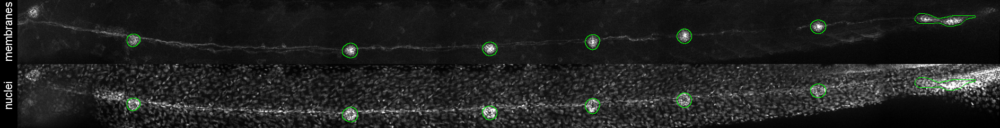
\includegraphics[width=0.9\linewidth]{figure/02-MaMo/GrTr/ClusterAnal/B06SB1P05_montage} 

}

\caption{Registered, Maximum Z projected data with cell cluster labels}\label{fig:maxllreg}
\end{figure}
\hypertarget{ground-truth-data}{%
\subparagraph{Ground Truth data}\label{ground-truth-data}}

Figure \ref{fig:countP05} shows the single registered cell clusters from figure 1 and the manually labeled nuclei within.


\begin{figure}

{\centering 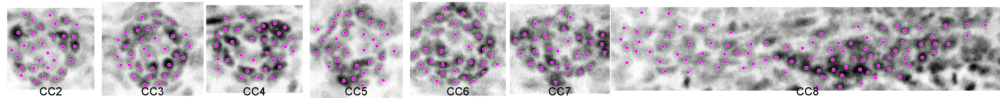
\includegraphics[width=0.9\linewidth]{figure/02-MaMo/GrTr/ClusterAnal/count_P05} 

}

\caption{Nuclei labels}\label{fig:countP05}
\end{figure}
\hypertarget{data-analysis}{%
\paragraph{Data Analysis}\label{data-analysis}}

\hypertarget{nuclei-count}{%
\subparagraph{Nuclei Count}\label{nuclei-count}}

Comparing the segmented objects count of the Gaussian parameters with the ground truth gives an indication for over- resp. under-segmentation. In figure \ref{fig:GrTratioCC} the relative numbers for each parameter can be seen in percentage above or below the mean cell count of the ground truth (blue horizon). The red area represents over-segmentation, the green under-segmentation. Additionally, table \ref{tab:meanabsnuc} shows the absolute numbers.


\begin{figure}

{\centering 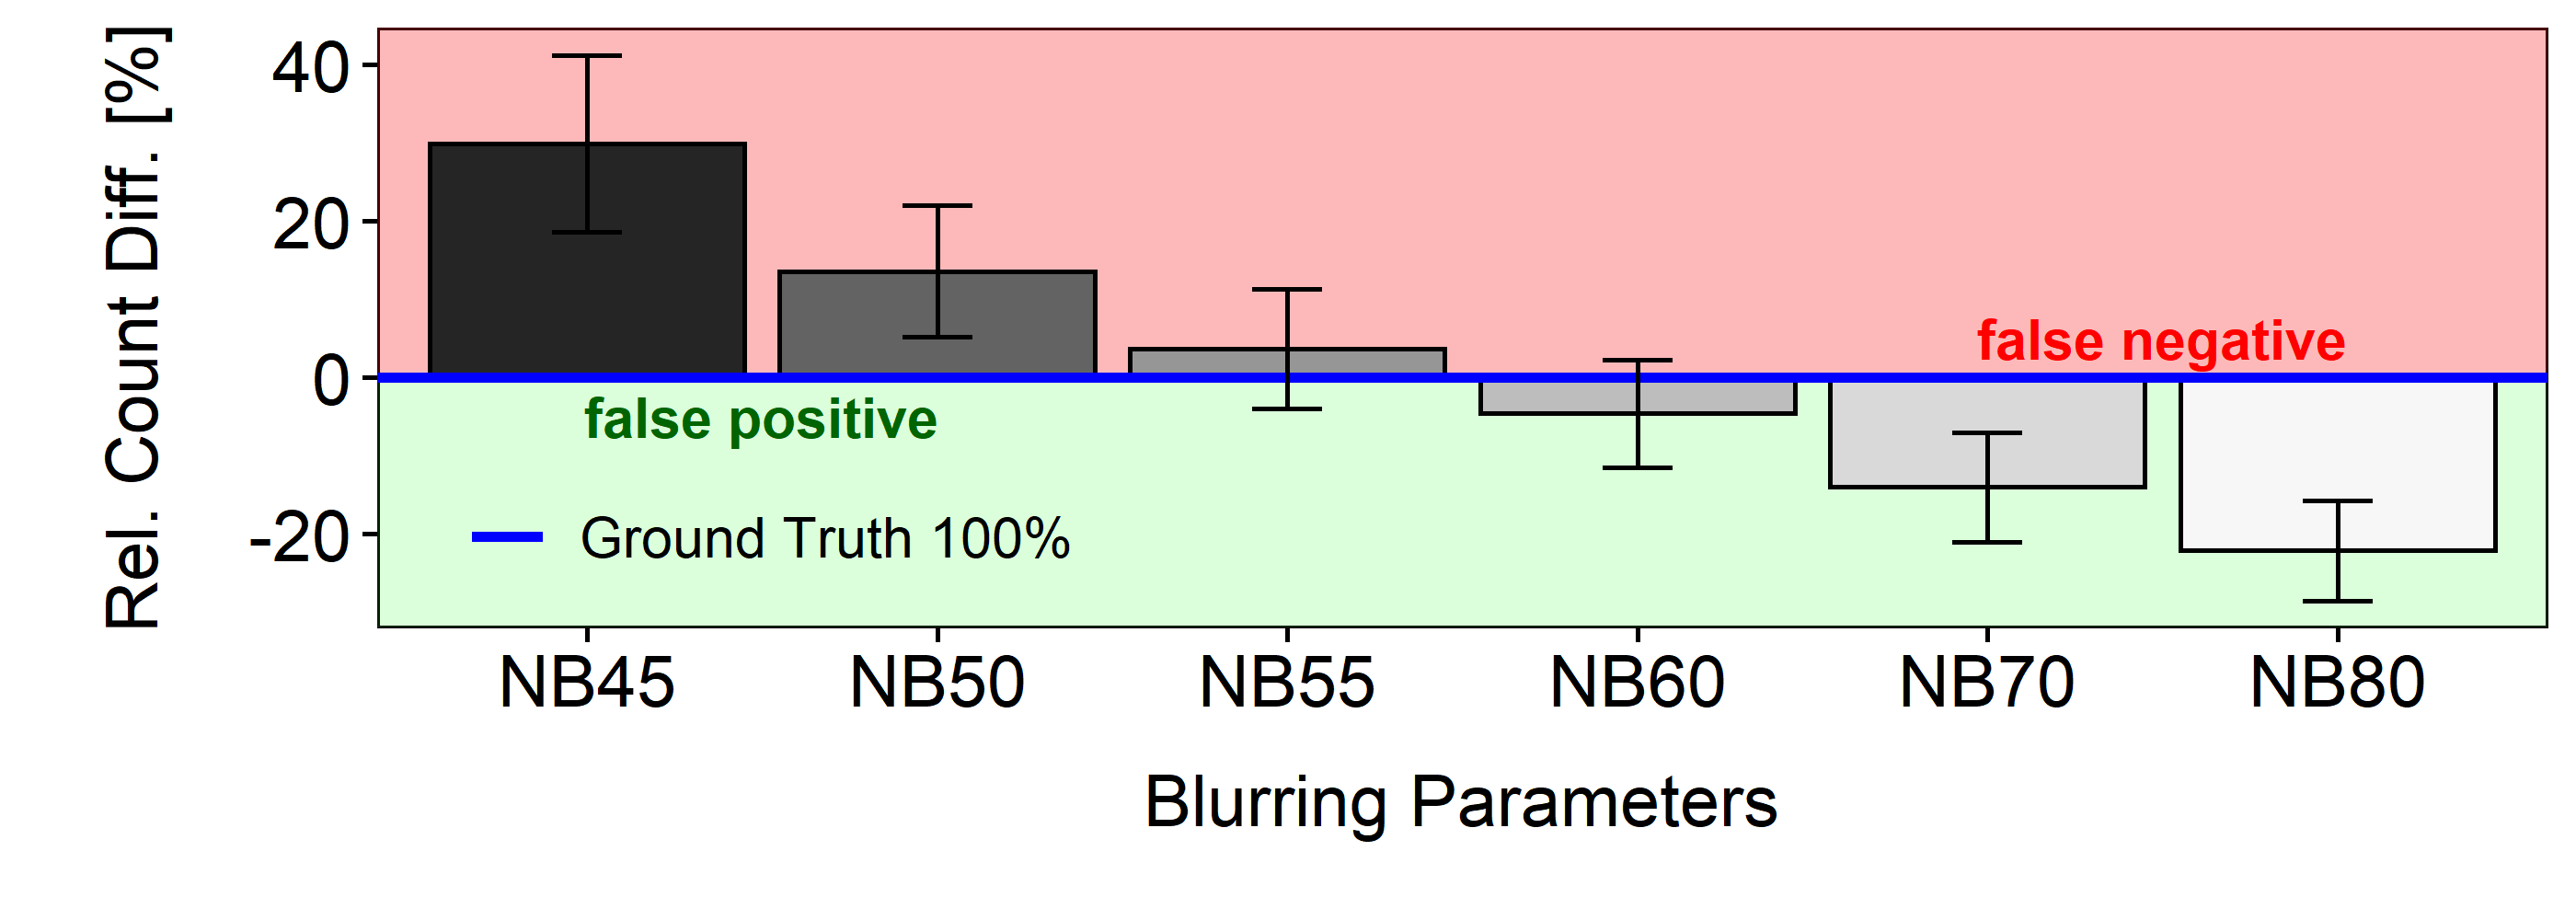
\includegraphics[width=0.65\linewidth]{thesis_files/figure-latex/GrTratioCC-1} 

}

\caption[Relative difference of segment counts]{Relative difference of segment counts (N=3, Errorbars = Std./2)}\label{fig:GrTratioCC}
\end{figure}
\begin{table}[t]

\caption{\label{tab:meanabsnuc}Nuclei count}
\centering
\begin{tabu} to \linewidth {>{\raggedright}X>{\raggedright}X>{\raggedright}X>{\raggedright}X>{\raggedright}X>{\raggedright}X>{\raggedright}X>{\raggedright}X}
\toprule
  & GrT & NB45 & NB50 & NB55 & NB60 & NB70 & NB80\\
\midrule
\rowcolor{gray!6}  Mean\_Nuclei & 40.95 & 52.81 & 45.76 & 41.90 & 38.57 & 34.62 & 31.33\\
STD. & 21.53 & 27.90 & 22.03 & 20.51 & 18.75 & 16.34 & 14.78\\
\bottomrule
\end{tabu}
\end{table}
\noindent To estimate the quality of nuclei detection for each parameter, the ratio of automatically detected and ground truth objects count can be calculated and compared (table \ref{tab:nrcount}). The closer it is to 1, the better.
\begin{table}[t]

\caption{\label{tab:nrcount}Nuclei count ratio}
\centering
\begin{tabu} to \linewidth {>{\raggedright}X>{\raggedright}X>{\raggedright}X>{\raggedright}X>{\raggedright}X>{\raggedright}X}
\toprule
  & NB45 & NB50 & NB55 & NB60 & NB70\\
\midrule
\rowcolor{gray!6}  Mean\_ratio & 1.30 & 1.14 & 1.04 & 0.95 & 0.86\\
STD. & 0.23 & 0.17 & 0.15 & 0.14 & 0.14\\
\bottomrule
\end{tabu}
\end{table}
\hypertarget{summary-1}{%
\paragraph{Summary}\label{summary-1}}

Maximum performance is achieved at a scaled parameter of 6 \(\mu\)m, with a ratio of of 0.95 for the count objects and a standard deviation of 0.14.

\hypertarget{d-ground-truth-1}{%
\subsubsection{3-D Ground Truth}\label{d-ground-truth-1}}

\hypertarget{ground-truth-design-1}{%
\paragraph{Ground Truth Design}\label{ground-truth-design-1}}

To assess the quality of the PLLpANALYZER3D algorithm the ground truth was designed as follows.

\hypertarget{model-1}{%
\subparagraph{Model}\label{model-1}}
\begin{itemize}
\tightlist
\item
  each PLLp consists of a number of objects (cells)
\item
  each object is part of the PLLp and defines one cell entity
\item
  cell boundaries are determined via the transgene \emph{cldnb:lyn-gfp} +/+
\item
  embryos are imaged live to conserve signal and membrane integrity
\item
  embryos are mounted within a 3D mold for improved 3D alignment
\end{itemize}
\begin{longtable}[]{@{}cl@{}}
\caption{\label{tab:model3DGrT} PLLpANALYZER3D Model}\tabularnewline
\toprule
\endhead
\begin{minipage}[t]{0.23\columnwidth}\centering
Exposure time\strut
\end{minipage} & \begin{minipage}[t]{0.71\columnwidth}\raggedright
100 ms\strut
\end{minipage}\tabularnewline
\begin{minipage}[t]{0.23\columnwidth}\centering
Laser intensity\strut
\end{minipage} & \begin{minipage}[t]{0.71\columnwidth}\raggedright
100\% / 9.3 mW\strut
\end{minipage}\tabularnewline
\begin{minipage}[t]{0.23\columnwidth}\centering
Objective\strut
\end{minipage} & \begin{minipage}[t]{0.71\columnwidth}\raggedright
40X; Nikon CFI APO LWD WI; N.A. = 1.15, W.D. = 0.60 mm\strut
\end{minipage}\tabularnewline
\begin{minipage}[t]{0.23\columnwidth}\centering
Z-spacing\strut
\end{minipage} & \begin{minipage}[t]{0.71\columnwidth}\raggedright
0.4 - 0.5 \(\mu\)m\strut
\end{minipage}\tabularnewline
\begin{minipage}[t]{0.23\columnwidth}\centering
Camera\strut
\end{minipage} & \begin{minipage}[t]{0.71\columnwidth}\raggedright
Andor ZYLA PLUS sCMOS; 4.2 M.Pix; 82\% Q.E.\strut
\end{minipage}\tabularnewline
\begin{minipage}[t]{0.23\columnwidth}\centering
SD system\strut
\end{minipage} & \begin{minipage}[t]{0.71\columnwidth}\raggedright
Yokogawa CSU - W1; 50 \(\mu\)m pattern\strut
\end{minipage}\tabularnewline
\begin{minipage}[t]{0.23\columnwidth}\centering
Piezo\strut
\end{minipage} & \begin{minipage}[t]{0.71\columnwidth}\raggedright
Piezo Z-table; 300 \(\mu\)m scan range\strut
\end{minipage}\tabularnewline
\bottomrule
\end{longtable}
\hypertarget{training-data-1}{%
\subparagraph{Training data}\label{training-data-1}}

The training set consists of three randomly picked wildtype PLLps. For each the algorithm is run with no filters (X, Y, Z border objects, size) and a minimum segmentation threshold. Afterwards the segmentation result is corrected manually for over- and under-segmentation and objects that are not part of the PLLp.

\hypertarget{test-data-1}{%
\subparagraph{Test data}\label{test-data-1}}

To test the algorithm it is run at different segmentation thresholds on the same image data.

\hypertarget{image-analysis-1}{%
\paragraph{Image Analysis}\label{image-analysis-1}}

For image analysis a custom IJ macro script was developed that recognizes the cell boundaries via the fluorescence signal emitted by a Lyn Kinase tethered eGFP which expression is controlled by the \emph{cxcr4b} lateral line specific promotor. The central IJ tool used to do this is the MorphoLibJ's(\emph{49}) \emph{Morpholigical Segmentation} plugin. The plugin however requires to choose for a `segmentation threshold' that determines the quality and the quantity of segmented objects. This parameter therefore plays an essential role in the truthfulness of the analysis results.

\hypertarget{macro-modules-1}{%
\subparagraph{Macro modules}\label{macro-modules-1}}

The macro developed consists of the following main modules:
\begin{enumerate}
\def\labelenumi{\arabic{enumi}.}
\tightlist
\item
  PLLp registration and cropping in X, Y and Z
\item
  Image segmentation using the MorphoLibJ's(\emph{49}) \emph{Morpholigical Segmentation} plugin
\item
  Extration of 3-D measurements using the 3D ImageJ Suite's(\emph{50}) \emph{3D Manager} plugin
\item
  Cropping, clearing and measurement of single cell volumes using a custom IJ script
\end{enumerate}
\hypertarget{registration}{%
\subparagraph{Registration}\label{registration}}

The first module of the macro is PLLp registration in X, Y and cropping in Z. This is accomplished by an initial maximum Z projection and blurring of the image, 2-D segmentation using a minimum threshold and lastly by measuring the angle the segment is rotated against the horizon (at 0\(^{\circ}\)). After rotation the PLLp is then registered in Y and the image is cropped by drawing a rectangle with fixed height.

\hypertarget{unprocessed-data}{%
\subparagraph{Unprocessed data}\label{unprocessed-data}}


\begin{figure}

{\centering 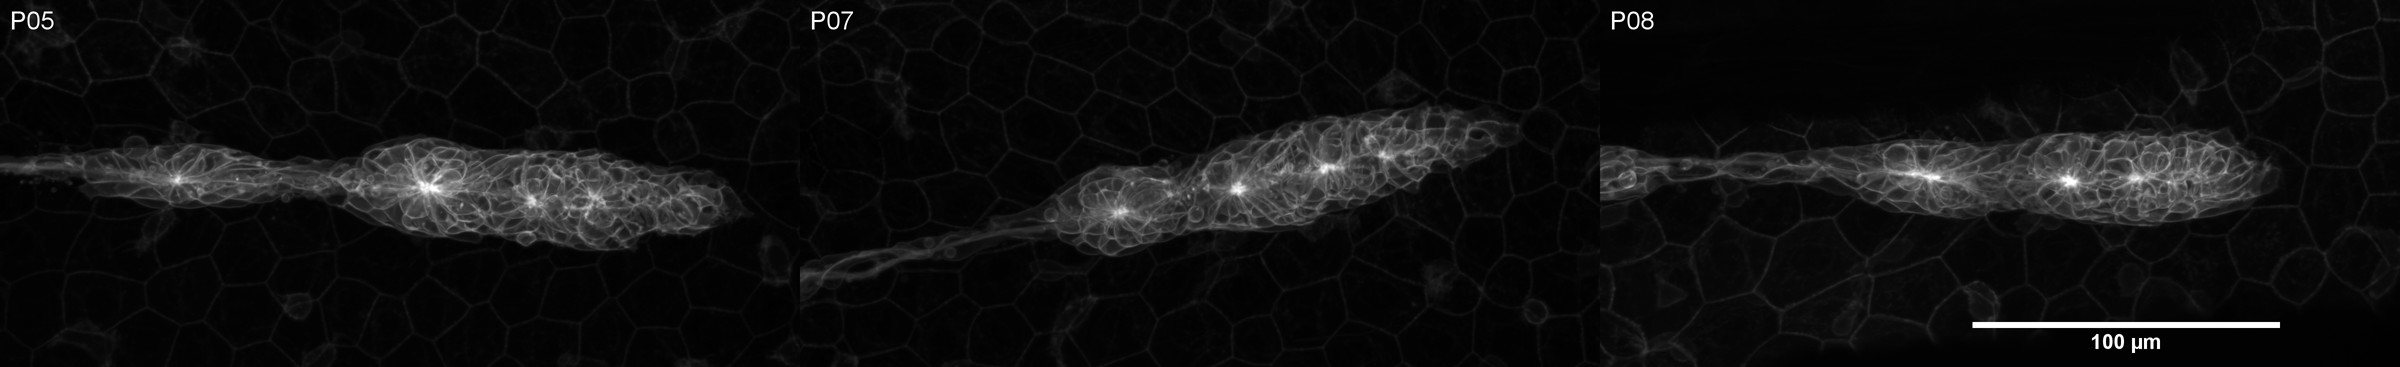
\includegraphics[width=0.9\linewidth]{figure/02-MaMo/GrTr/Morphology/zmax_comb_2} 

}

\caption{Unregistered, Maximum Z projected data}\label{fig:maxraw}
\end{figure}
\begin{longtable}[]{@{}rl@{}}
\caption{\label{tab:imgprop} Physical image properties (scaling)}\tabularnewline
\toprule
\endhead
\begin{minipage}[t]{0.46\columnwidth}\raggedleft
X / Y resolution\strut
\end{minipage} & \begin{minipage}[t]{0.46\columnwidth}\raggedright
0.1625 / 0.1625 \(\mu\)m\strut
\end{minipage}\tabularnewline
\begin{minipage}[t]{0.46\columnwidth}\raggedleft
Z resolution\strut
\end{minipage} & \begin{minipage}[t]{0.46\columnwidth}\raggedright
0.4 \(\mu\)m\strut
\end{minipage}\tabularnewline
\begin{minipage}[t]{0.46\columnwidth}\raggedleft
\(\Delta\)T - Z\strut
\end{minipage} & \begin{minipage}[t]{0.46\columnwidth}\raggedright
0.5428 s\strut
\end{minipage}\tabularnewline
\bottomrule
\end{longtable}
\hypertarget{registered-data-1}{%
\subparagraph{Registered data}\label{registered-data-1}}

During the registration process, the image is rotated against the horizon and cropped in X and Y. Additionally, the centers of the most constricting areas are detected via an intensity based dynamic threshold and highlighted as magenta circles in \ref{fig:maxreg}. Table \ref{tab:imgregpar} sums up the registration parameters.


\begin{figure}

{\centering 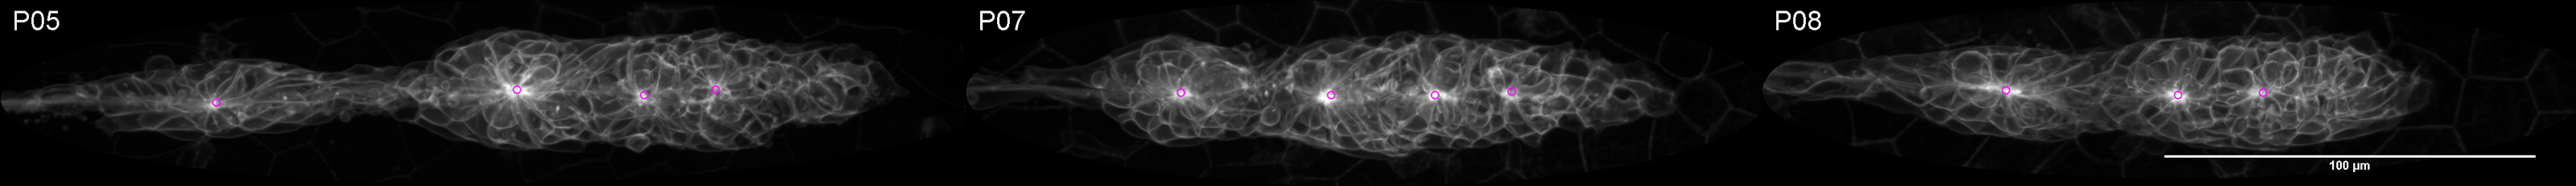
\includegraphics[width=0.95\linewidth]{figure/02-MaMo/GrTr/Morphology/zmax_reg_comb_2} 

}

\caption{Registered, Maximum Z projected data}\label{fig:maxreg}
\end{figure}
\begin{longtable}[]{@{}cccc@{}}
\caption{\label{tab:imgregpar} Registration parameters}\tabularnewline
\toprule
\begin{minipage}[b]{0.17\columnwidth}\centering
\textbf{Position}\strut
\end{minipage} & \begin{minipage}[b]{0.23\columnwidth}\centering
Angle of rotation\strut
\end{minipage} & \begin{minipage}[b]{0.26\columnwidth}\centering
Constriction centers\strut
\end{minipage} & \begin{minipage}[b]{0.23\columnwidth}\centering
Y registration\strut
\end{minipage}\tabularnewline
\midrule
\endfirsthead
\toprule
\begin{minipage}[b]{0.17\columnwidth}\centering
\textbf{Position}\strut
\end{minipage} & \begin{minipage}[b]{0.23\columnwidth}\centering
Angle of rotation\strut
\end{minipage} & \begin{minipage}[b]{0.26\columnwidth}\centering
Constriction centers\strut
\end{minipage} & \begin{minipage}[b]{0.23\columnwidth}\centering
Y registration\strut
\end{minipage}\tabularnewline
\midrule
\endhead
\begin{minipage}[t]{0.17\columnwidth}\centering
P05\strut
\end{minipage} & \begin{minipage}[t]{0.23\columnwidth}\centering
-4.4\(^{\circ}\)\strut
\end{minipage} & \begin{minipage}[t]{0.26\columnwidth}\centering
4\strut
\end{minipage} & \begin{minipage}[t]{0.23\columnwidth}\centering
168.25 px\strut
\end{minipage}\tabularnewline
\begin{minipage}[t]{0.17\columnwidth}\centering
P07\strut
\end{minipage} & \begin{minipage}[t]{0.23\columnwidth}\centering
12.3\(^{\circ}\)\strut
\end{minipage} & \begin{minipage}[t]{0.26\columnwidth}\centering
4\strut
\end{minipage} & \begin{minipage}[t]{0.23\columnwidth}\centering
188.35 px\strut
\end{minipage}\tabularnewline
\begin{minipage}[t]{0.17\columnwidth}\centering
P08\strut
\end{minipage} & \begin{minipage}[t]{0.23\columnwidth}\centering
0\(^{\circ}\)\strut
\end{minipage} & \begin{minipage}[t]{0.26\columnwidth}\centering
3\strut
\end{minipage} & \begin{minipage}[t]{0.23\columnwidth}\centering
153.83 px\strut
\end{minipage}\tabularnewline
\bottomrule
\end{longtable}
\hypertarget{segmentations}{%
\subsubsection{Segmentations}\label{segmentations}}

\hypertarget{membrane-signal}{%
\paragraph{Membrane signal}\label{membrane-signal}}

Watershed segmentation depends on a continuous signal along the boundary of the object to be segmented. Since the PLLp lies within the zebrafish larvae and since light gets scattered more when traveling through more organic tissues, the fluorescence signal in deeper tissue sections is more disturbed. Still, the PLLp is located just superficial to the skin, so the effect may be minor. In figure \ref{fig:stackmem} the fluorescence signal of the three PLLps tested is shown in a single central cross-section in the dorso-ventral and the apico-basal axis.


\begin{figure}

{\centering 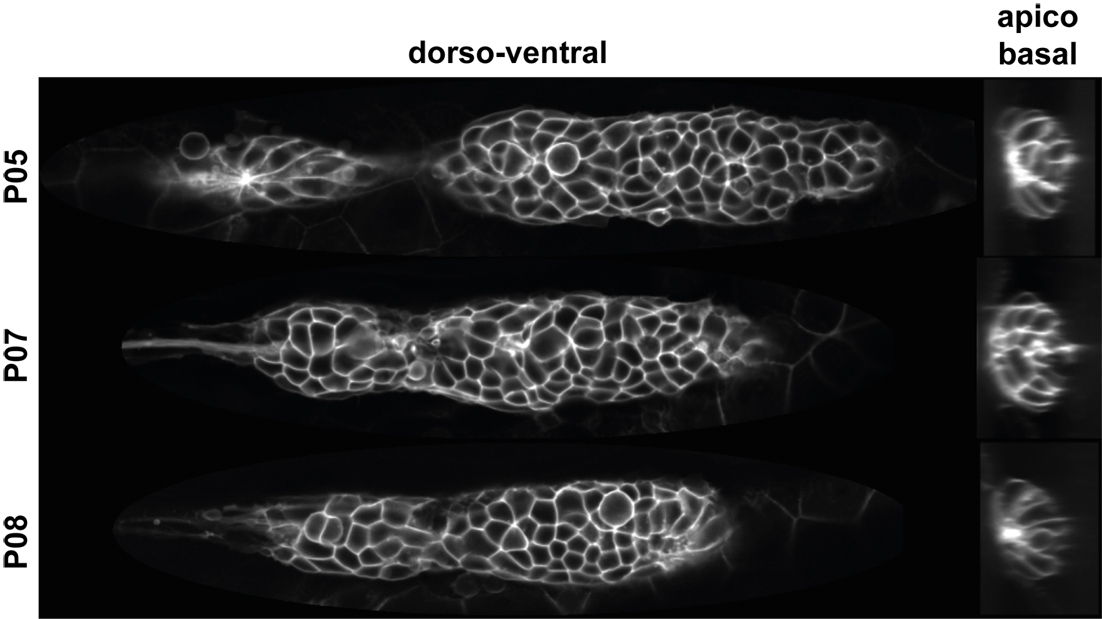
\includegraphics[width=0.5\linewidth]{figure/02-MaMo/GrTr/Morphology/signals} 

}

\caption{Signal intensities in XY and YZ at central cross-sections}\label{fig:stackmem}
\end{figure}
\hypertarget{ground-truth-threshold-segments}{%
\paragraph{Ground Truth \& Threshold segments}\label{ground-truth-threshold-segments}}

To compare the results between the ground truth segments and the segments obtained from different threshold levels graphically, for a single PLLp the ground truth and threshold level{[}n{]} are shown as a composite color image in figure \ref{fig:stackcomp}. By using a green lookup table (LUT) for the ground truth and a magenta LUT for the threshold level{[}n{]}, one can readily detect overlapping objects (white), over segmentation (magenta) and under segmentation (green).


\begin{figure}

{\centering 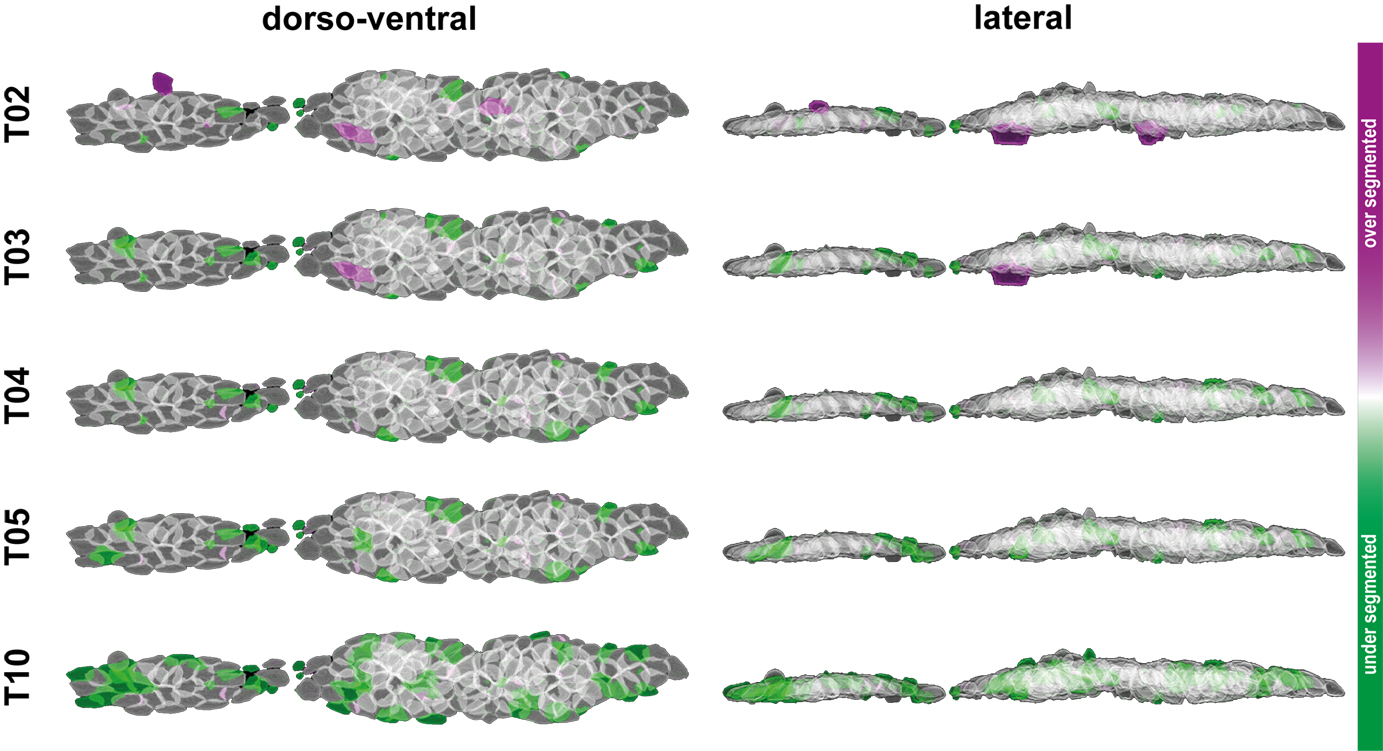
\includegraphics[width=0.85\linewidth]{figure/02-MaMo/GrTr/Morphology/volumes} 

}

\caption{Graphical comparison of the thresholds tested}\label{fig:stackcomp}
\end{figure}
\noindent Volume renderings have been done with IJ's \href{\%22https://github.com/fiji/Volume_Viewer/releases/tag/Volume_Viewer-2.01.2\%22}{VolumeViewer}

\hypertarget{data-analysis-1}{%
\subsubsection{Data Analysis}\label{data-analysis-1}}

\hypertarget{cell-count}{%
\paragraph{Cell Count}\label{cell-count}}

In figure \ref{fig:gtratio} the relative numbers for each threshold level can be seen in percentage above or below the mean cell count of the ground truth (blue horizon). Analogous to the graphical inspection, the magenta area represents over segmentation, the green under segmentation. Additionally, table \ref{tab:gtrcellcount} shows the absolute numbers.


\begin{figure}

{\centering 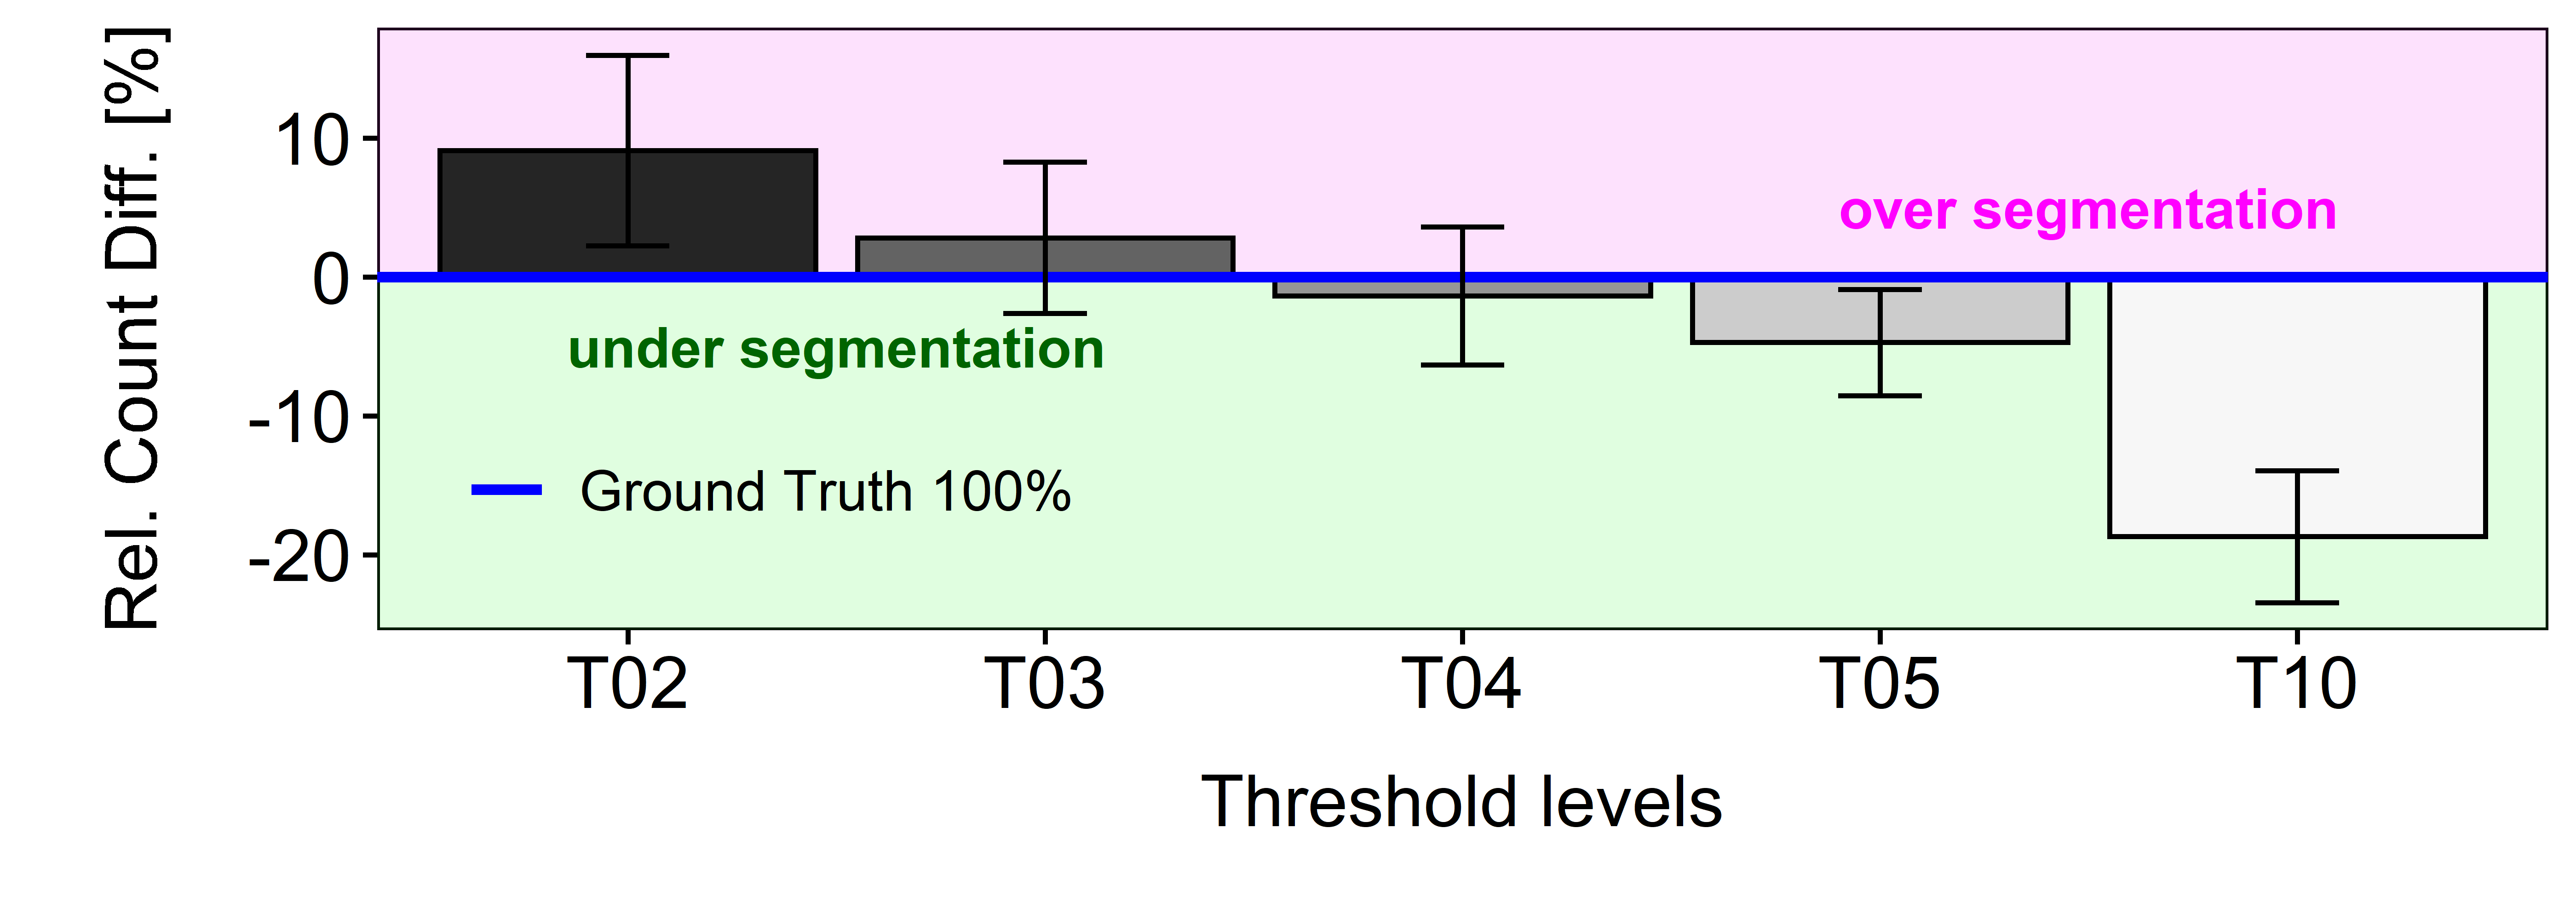
\includegraphics[width=0.65\linewidth]{thesis_files/figure-latex/gtratio-1} 

}

\caption[Relative difference of segment counts]{Relative difference of segment counts (N=3, Errorbars = Std./2)}\label{fig:gtratio}
\end{figure}
\begin{longtable}[]{@{}ccccccc@{}}
\caption{\label{tab:gtrcellcount} Absolute numbers}\tabularnewline
\toprule
\endhead
\textbf{Group} & T01\_GrT & T02 & T03 & T04 & T05 & T10\tabularnewline
\textbf{P05} & 146 & 139 & 133 & 131 & 131 & 117\tabularnewline
\textbf{P07} & 150 & 184 & 169 & 164 & 156 & 137\tabularnewline
\textbf{P08} & 127 & 139 & 133 & 123 & 117 & 92\tabularnewline
\bottomrule
\end{longtable}
\hypertarget{cell-morphology}{%
\paragraph{Cell Morphology}\label{cell-morphology}}
\begin{quote}
\emph{There is always a precision / recall trade-off in detection tasks, e.g., when we set a lower threshold {[}. . .{]}, we can get a higher recall with a lower precision ({[}. . .{]}, but meanwhile we also get more false-positives in the results).}(\emph{41})
\end{quote}
Inspecting the cell count unfortunately does not directly tell us how well the cell morphology is conserved at different threshold levels, since at higher threshold levels the cell boundaries are differently determined and eventually not even recognized as such anymore.

\noindent The volume of a cell is a very robust morphological feature. Therefore, if its volume does not differ significantly at a given threshold level we consider its morphology to be conserved.

\hypertarget{sample-distribution}{%
\subsubsection{Sample distribution}\label{sample-distribution}}

In figure \ref{fig:volsecdffull} and \ref{fig:volsecdfzoom} the distribution and amount of the cell volumes across the different threshold levels can be inspected via the `empirical cumulative distribution function' (ECDF). The closer the slopes are to the ground truth, the stronger they are conserved. Figure \ref{fig:volsecdffull} shows the full distribution, where the major differences seem to appear within the 0.4 quantile (red line). Therefore, in figure \ref{fig:volsecdfzoom} only the values within the 0.4 quantile are shown to get a more detailed impression.


\begin{figure}

{\centering 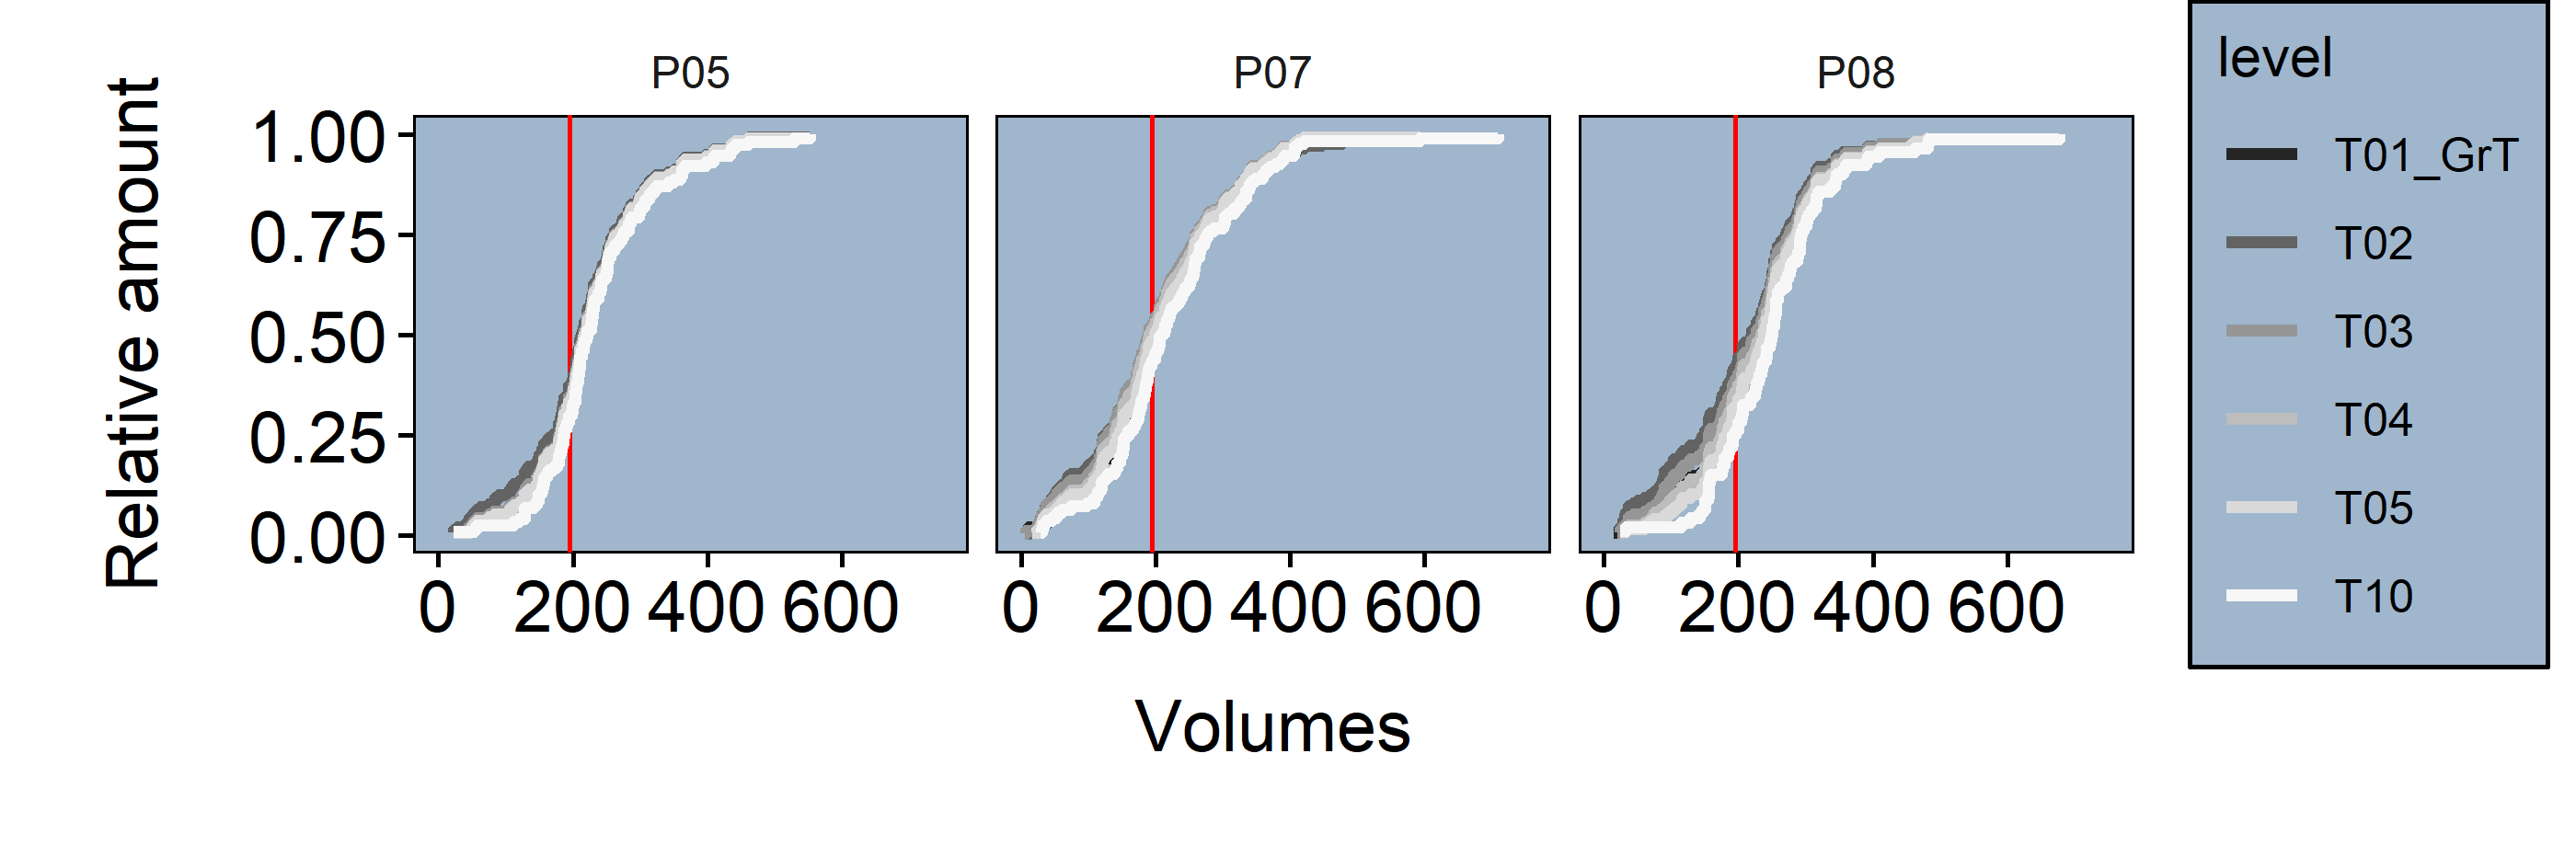
\includegraphics[width=0.9\linewidth]{thesis_files/figure-latex/volsecdffull-1} 

}

\caption{ECDF - All cell volumes}\label{fig:volsecdffull}
\end{figure}

\begin{figure}

{\centering 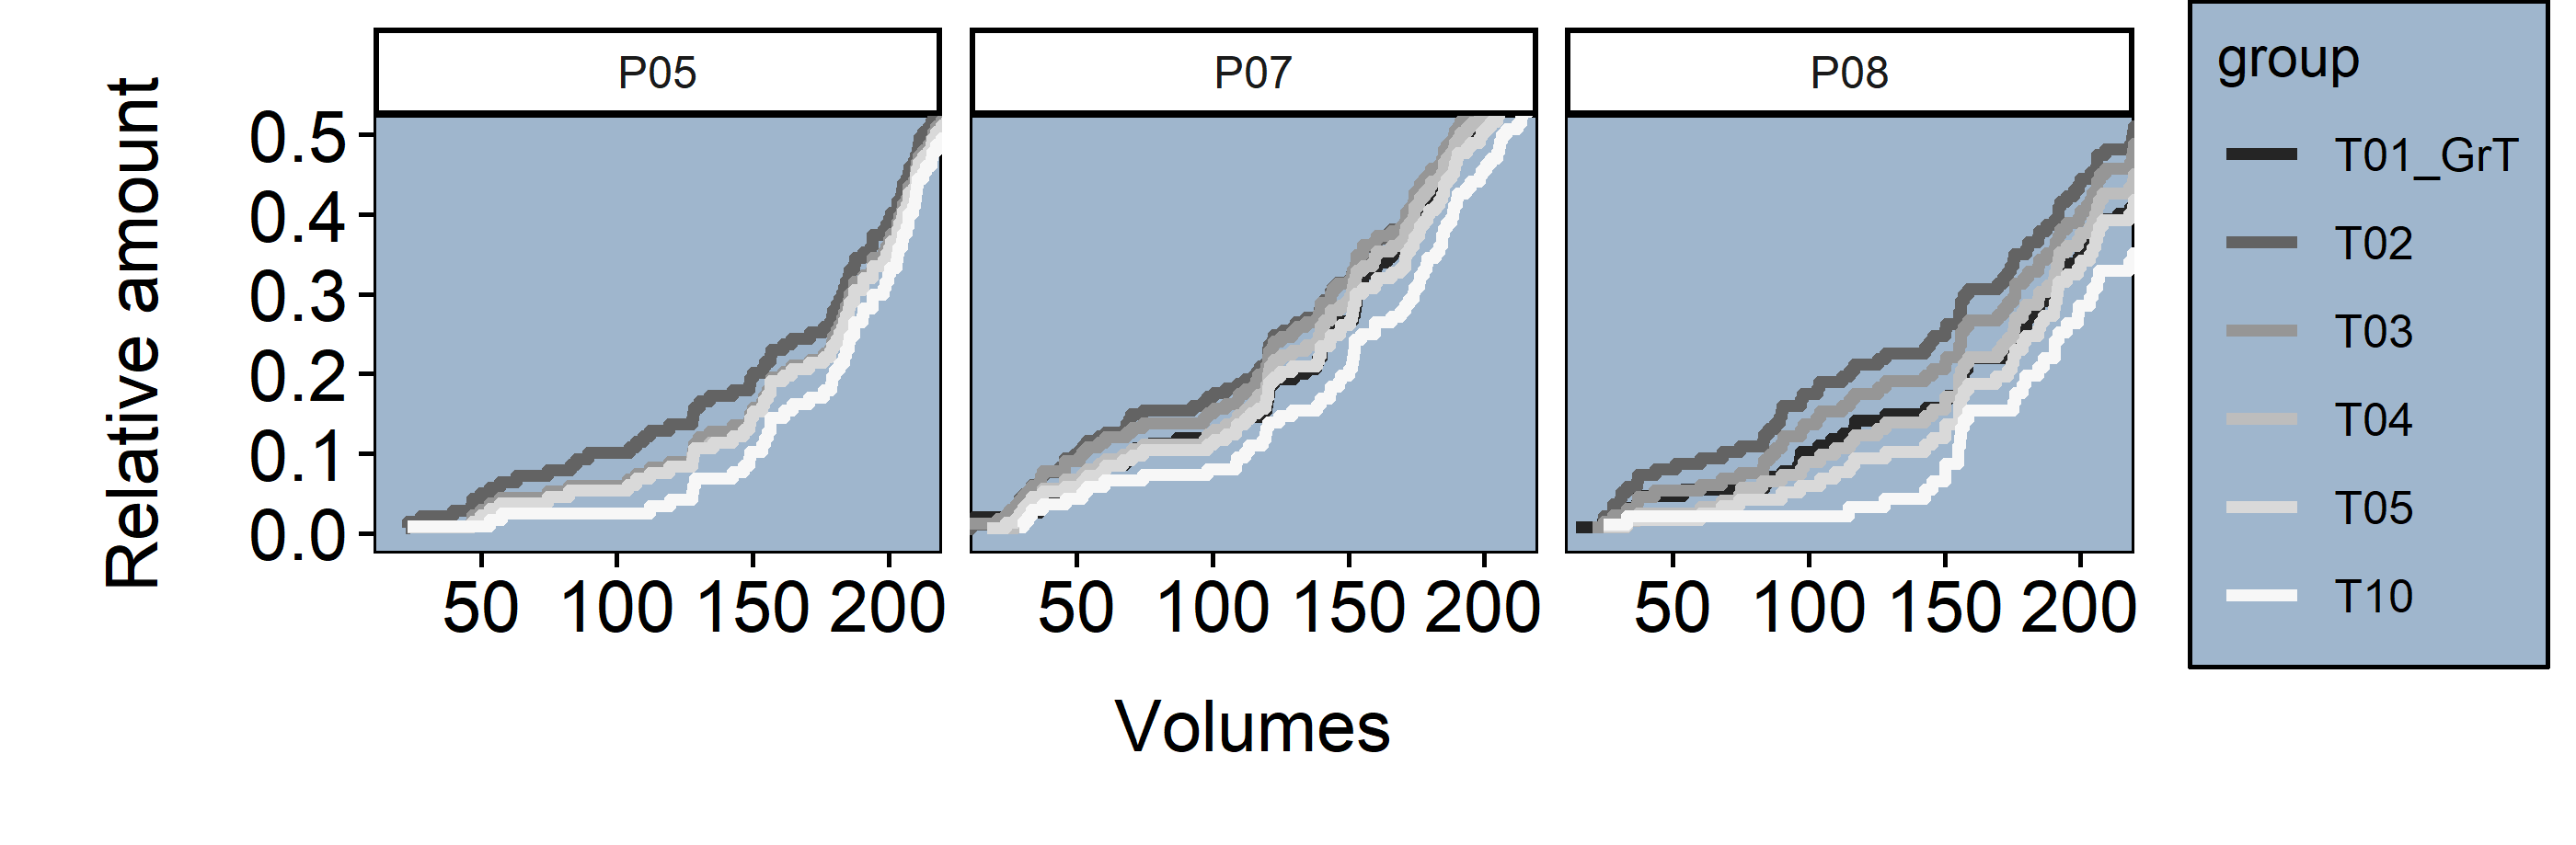
\includegraphics[width=0.9\linewidth]{thesis_files/figure-latex/volsecdfzoom-1} 

}

\caption{ECDF - Small cell volumes}\label{fig:volsecdfzoom}
\end{figure}
\hypertarget{confidence-level}{%
\subsubsection{Confidence level}\label{confidence-level}}

To statistically check how closely related each threshold value sample distribution is compared to the ground truth, a Kolmogorov-Smirnov-Test (ks.test) was performed. The ks.test is a nonparametric test whose null hypothesis is that the both groups compared were sampled from populations with identical populations. Therefore, the closer the p-value is to 1, the more similar the tested sample distribution would be to the ground truth (figure \ref{fig:kstestvol}; 5\% confidence threshold indicated by red line).

\[H_{0} : F_X(x)=F_0(x)\]


\begin{figure}

{\centering 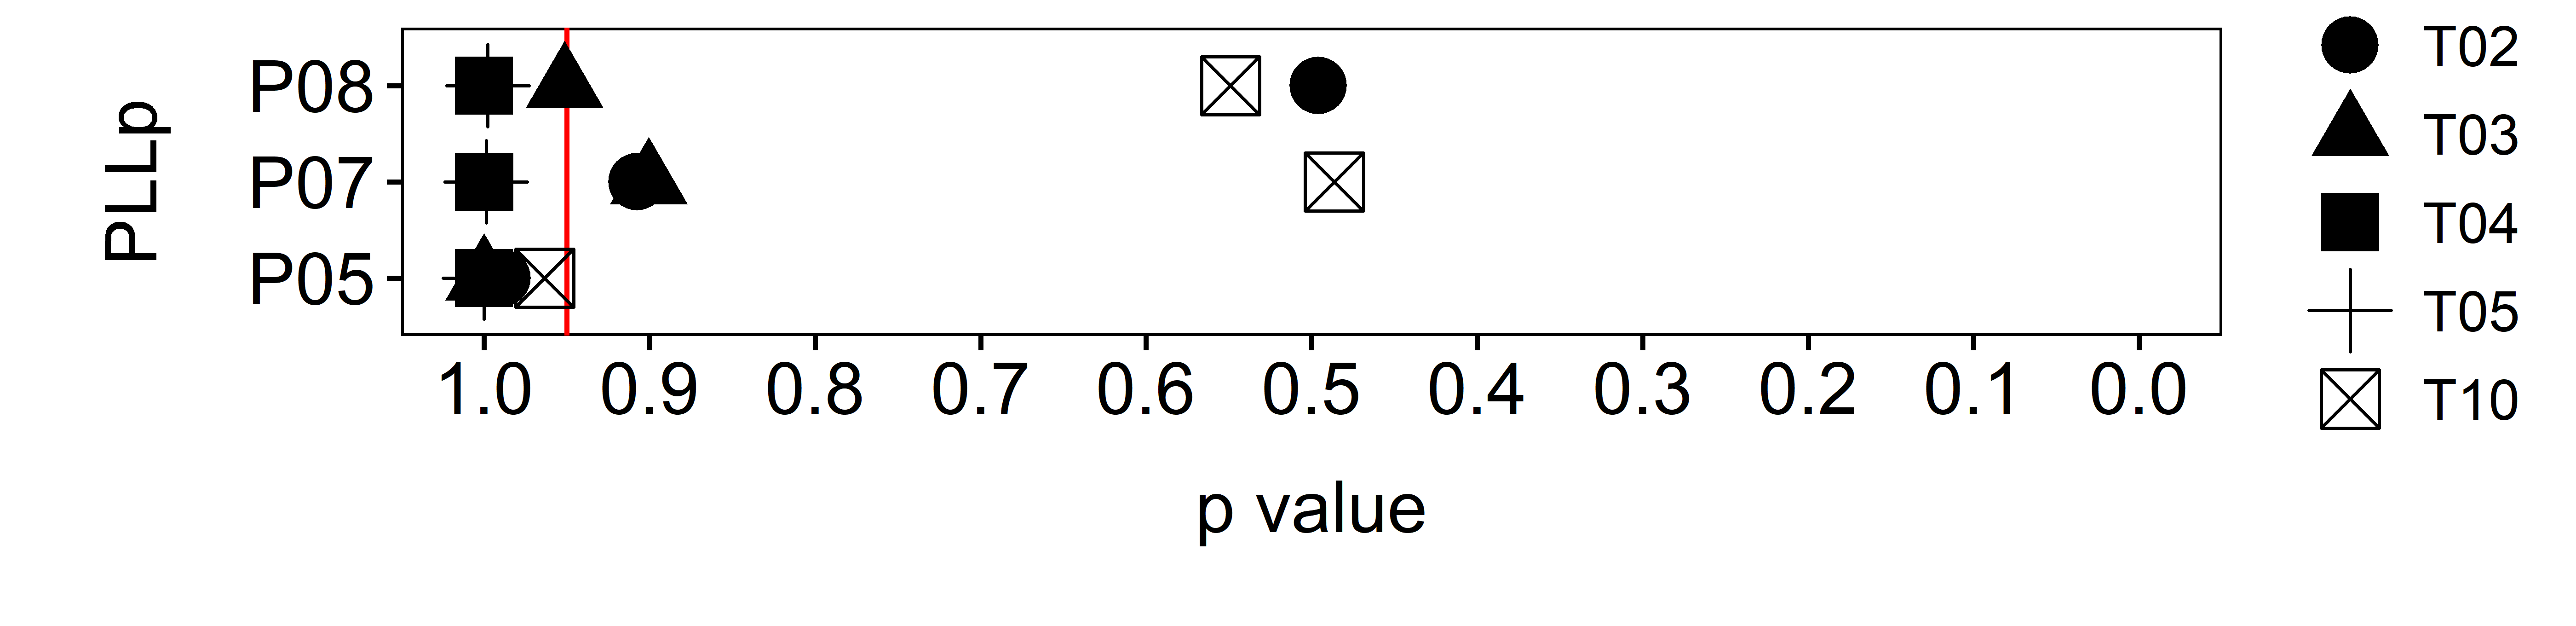
\includegraphics[width=0.6\linewidth]{thesis_files/figure-latex/kstestvol-1} 

}

\caption{Volumetric conservation confidence level}\label{fig:kstestvol}
\end{figure}
\noindent In comparison to the Mann-Whitney test, the ks.test is more sensitive to detect changes in the shape of the distribution than to detect a shift of the median(\emph{51})

\hypertarget{summary-2}{%
\paragraph{Summary}\label{summary-2}}

For the cell count

\hypertarget{met}{%
\section{Methods}\label{met}}

\hypertarget{Zeb-met}{%
\subsection{Zebrafish}\label{Zeb-met}}

\hypertarget{husbandry}{%
\subsubsection{Husbandry}\label{husbandry}}

The zebrafish husbandry is maintained at the University of Frankfurt am Main. All the legal procedures were followed while handling and maintaining the zebrafish husbandry. All the zebrafish lines used in and generated for this study are listed in the Appendix A.

\hypertarget{handling-and-rearing}{%
\subsubsection{Handling and rearing}\label{handling-and-rearing}}

12 h before the embryo collection, males and females are set up in crossing cages filled \textasciitilde{}75. Next day, before noon, separators are removed and eggs are laid. The zebrafish eggs are then collected and reared untill the larval stage (Day 5) in the well-defined culture medium E3 (Kimmel et.al. 1995, Table no. 6 in `List of Buffers' section) at 25, 28.5, or 30 degrees celsius, according to the need of experiments.

To grow larvae to the adulthood, they were transferred to the system on day 5. Till day 12, larvae were fed Vinegar Eels, Paramecia, and Caviar powder. After the 12 th day, water supply was started and fish were fed Brine Shrimp, Artemia, Paramecia and Vinegar Eels. Adult fish (\textgreater{}1 Month) were fed Artemia and the dry flakes.

\hypertarget{zebrafish-fin-clips}{%
\subsubsection{Zebrafish fin clips}\label{zebrafish-fin-clips}}

Adult fish were anesthetized with buffered Tricaine (1X, see `List of Buffers') until stage II-III of anaestezia. About 1/3 rd of the pectoral fin was cut with a sterile scalpel in a sterile petri plate. Immediately the cut fin was transferred to 50 mM NaOH. Fish were returned to system water and kept in the single tanks with 200 micro liters of 0.01 percent methylen blue, maximum up to 4 days.

\hypertarget{adult-genotyping}{%
\subsubsection{Adult Genotyping}\label{adult-genotyping}}

The clipped fins were digested for 1 h at 95 degrees celsius and neutralized subsequently with 1M Tris-HCl of pH 9.

\hypertarget{embryo-genotyping}{%
\subsubsection{Embryo Genotyping}\label{embryo-genotyping}}

Single fixed/live embryos were denatured at 95 degrees Celsius in 50mM NaOH for 1 hour and neutralized by adding 1/10 th volume of 1 M Tris-HCl (pH 8.2).

\hypertarget{zebrafish-euthanasia}{%
\subsubsection{Zebrafish Euthanasia}\label{zebrafish-euthanasia}}

Adult zebrafish were anesthetized in tricaine (1X) till stage II-III of anaestezia and put in the ice cold water so as to sacrifice them by hypothermia.

\hypertarget{fixation}{%
\subsubsection{Fixation}\label{fixation}}

Embryos and dechorionated larvae were fixed in 2 ml of 4 PFA in 1X PBS overnight at 4 degrees Celsius.

\hypertarget{Wet-met}{%
\subsection{Wetlab Methods}\label{Wet-met}}

\hypertarget{ISH-met}{%
\subsubsection{In Situ Hybridization}\label{ISH-met}}

\hypertarget{breeding-fixation}{%
\paragraph{0. Breeding \& Fixation}\label{breeding-fixation}}
\begin{itemize}
\tightlist
\item
  Embryos are grown till desired stage
  \begin{itemize}
  \tightlist
  \item
    from 24 hpf on in 1X PTU
  \end{itemize}
\item
  Dechorionation in 0.1 mg/mL Pronase
  \begin{itemize}
  \tightlist
  \item
    150 \(\mu\)L per 10 mL for \textasciitilde{}30 min.
  \item
    For embryos younger than 18s, keep embryos in solution while washing and gently add fresh E3
  \end{itemize}
\item
  Fixation at desired stage in 4\% PFA in 0.1\% PBST at 4\(^\circ\)C o.n.
\item
  Rinse 3x5 min. in PBST
\item
  Pass through MeOH series (25\% \(\rightarrow\) 50\% \(\rightarrow\) 75\% \(\rightarrow\) 100\% MeOH/PBST (V/V))
\item
  Store in 100\% MeOH at -20\(^\circ\)C for \textgreater{} 2h
\end{itemize}
\hypertarget{permeabilisation-probe-hybridization}{%
\paragraph{\texorpdfstring{1. Permeabilisation \& Probe Hybridization \newline \newline}{1. Permeabilisation \& Probe Hybridization }}\label{permeabilisation-probe-hybridization}}

\textbf{Permeabilisation} \newline \(\rightarrow\) without shaking
\begin{itemize}
\tightlist
\item
  Rehydrate embryos (75\% \(\rightarrow\) 50\% \(\rightarrow\) 25\% \(\rightarrow\) 0\% PBST)
\item
  Wash 2x in PBST
\item
  Digest embryos in 10 \(\mu\)g/mL Proteinase K according to table
\end{itemize}
\begin{longtable}[]{@{}lccccccccc@{}}
\caption{\label{tab:met-protk} Proteinase K digestion}\tabularnewline
\toprule
\begin{minipage}[b]{0.07\columnwidth}\raggedright
\textbf{Stage}\strut
\end{minipage} & \begin{minipage}[b]{0.07\columnwidth}\centering
0-6 s\strut
\end{minipage} & \begin{minipage}[b]{0.07\columnwidth}\centering
7 s\strut
\end{minipage} & \begin{minipage}[b]{0.07\columnwidth}\centering
18 s\strut
\end{minipage} & \begin{minipage}[b]{0.07\columnwidth}\centering
24 hpf\strut
\end{minipage} & \begin{minipage}[b]{0.07\columnwidth}\centering
32 hpf\strut
\end{minipage} & \begin{minipage}[b]{0.07\columnwidth}\centering
36 hpf\strut
\end{minipage} & \begin{minipage}[b]{0.07\columnwidth}\centering
42 hpf\strut
\end{minipage} & \begin{minipage}[b]{0.07\columnwidth}\centering
48 hpf\strut
\end{minipage} & \begin{minipage}[b]{0.07\columnwidth}\centering
72 hpf\strut
\end{minipage}\tabularnewline
\midrule
\endfirsthead
\toprule
\begin{minipage}[b]{0.07\columnwidth}\raggedright
\textbf{Stage}\strut
\end{minipage} & \begin{minipage}[b]{0.07\columnwidth}\centering
0-6 s\strut
\end{minipage} & \begin{minipage}[b]{0.07\columnwidth}\centering
7 s\strut
\end{minipage} & \begin{minipage}[b]{0.07\columnwidth}\centering
18 s\strut
\end{minipage} & \begin{minipage}[b]{0.07\columnwidth}\centering
24 hpf\strut
\end{minipage} & \begin{minipage}[b]{0.07\columnwidth}\centering
32 hpf\strut
\end{minipage} & \begin{minipage}[b]{0.07\columnwidth}\centering
36 hpf\strut
\end{minipage} & \begin{minipage}[b]{0.07\columnwidth}\centering
42 hpf\strut
\end{minipage} & \begin{minipage}[b]{0.07\columnwidth}\centering
48 hpf\strut
\end{minipage} & \begin{minipage}[b]{0.07\columnwidth}\centering
72 hpf\strut
\end{minipage}\tabularnewline
\midrule
\endhead
\begin{minipage}[t]{0.07\columnwidth}\raggedright
min.\strut
\end{minipage} & \begin{minipage}[t]{0.07\columnwidth}\centering
0\strut
\end{minipage} & \begin{minipage}[t]{0.07\columnwidth}\centering
4\strut
\end{minipage} & \begin{minipage}[t]{0.07\columnwidth}\centering
6\strut
\end{minipage} & \begin{minipage}[t]{0.07\columnwidth}\centering
15\strut
\end{minipage} & \begin{minipage}[t]{0.07\columnwidth}\centering
30\strut
\end{minipage} & \begin{minipage}[t]{0.07\columnwidth}\centering
40\strut
\end{minipage} & \begin{minipage}[t]{0.07\columnwidth}\centering
50\strut
\end{minipage} & \begin{minipage}[t]{0.07\columnwidth}\centering
60\strut
\end{minipage} & \begin{minipage}[t]{0.07\columnwidth}\centering
60\strut
\end{minipage}\tabularnewline
\bottomrule
\end{longtable}
\begin{itemize}
\tightlist
\item
  Wash 2x in PBST
\item
  PostFix in 4\% PFA at 4\(^\circ\)C for \textgreater{} 30 min.
\item
  Wash 3x in PBST
\end{itemize}
\textbf{Probe Hybridisation} \newline \(\rightarrow\) all steps at 60\(^\circ\)C, except stated differently
\begin{itemize}
\tightlist
\item
  Prehybridise in 350 \(\mu\)L of Hyb buffer for 1 - 8 h
\item
  Heat the probe in 200 \(\mu\)L of Hyb to 80\(^\circ\)C, then replace Hyb buffer with it
\item
  Incubate o.n.
\end{itemize}
\hypertarget{probe-removal-antibody-incubation}{%
\paragraph{2. Probe removal \& Antibody incubation}\label{probe-removal-antibody-incubation}}
\begin{itemize}
\tightlist
\item
  Collect probe \newline \(\rightarrow\) For reuse, store at -20\(^\circ\)C
\item
  Wash at the same temperature as hybridisation \newline \(\rightarrow\) use Thermo-Block and waterbath or oven to keep solutions at temperature
  \begin{itemize}
  \tightlist
  \item
    1 x 20 min. Hyb buffer
  \item
    2 x 30 min. 50\% Formamide
  \item
    1 x 20 min. 25\% Formamide
  \item
    2 x 15 min. 2X SSCT
  \item
    2 x 30 min. 0.2X SSCT
  \item
    1 x 5 min. TNT
  \end{itemize}
\item
  Block for 1 - 8 h in 350 \(\mu\)L of 2\% BR/TNT at RT
\item
  Incubate in 100 \(\mu\)L antibody in 2\% BR/TNT for 2 h at RT or o.n. at 4\(^\circ\)C
  \begin{itemize}
  \tightlist
  \item
    antibody = Anti-Digoxigenin (1/4000 (V/V))
  \item
    diluent = NTMT buffer
  \end{itemize}
\end{itemize}
\hypertarget{probe-detection}{%
\paragraph{3. Probe detection}\label{probe-detection}}
\begin{itemize}
\tightlist
\item
  Wash 6 x 20 min. in TNT (or one wash o.n.)
\item
  Wash 2 x 5 min. in NTMT
\item
  Replace with\ldots{}
  \begin{itemize}
  \tightlist
  \item
    4.5 NBT \(\mu\)L + 3.5 \(\mu\)L BCIP per mL NTMT or
  \item
    150 \(\mu\)L BM Purple
  \end{itemize}
\item
  Develop at RT in the dark without shaking \newline \(\rightarrow\) 2 - 8 h depending on probe
\item
  Wash 3x in PBST
\item
  If necessary, proceed to immunostaining
\item
  For permanent storage, keep specimen in 50\% Glycerol at 4\(^\circ\)C
\end{itemize}
\hypertarget{immuno-met}{%
\subsubsection{Immuno staining}\label{immuno-met}}
\begin{itemize}
\tightlist
\item
  Breeding and Fixation as for ISH
\item
  Block for 30 min. in 2\% Goat Serum / PBDT (V/V)
\item
  Primary Antibody
  \begin{itemize}
  \tightlist
  \item
    Incubate for 2 h at RT (or o.n. at 4\(^\circ\)C) in 150 \(\mu\)L of 2\% NGS / PBDT (V/V)
  \item
    Wash in PBDT for 2 h (change solution \textasciitilde{}6x)
  \end{itemize}
\item
  Secondary Antibody
  \begin{itemize}
  \tightlist
  \item
    Incubate for 2 h at RT (or o.n. at 4\(^\circ\)C) in 150 \(\mu\)L of 2\% NGS / PBDT (V/V)
  \item
    Wash in PBDT for 2 h (change solution \textasciitilde{}6x)
  \end{itemize}
\end{itemize}
\hypertarget{mount-met}{%
\subsubsection{Mounting}\label{mount-met}}

For mounting, an improved 3D specimen preparation and well-plate like sample navigation for zebrafish larvae confocal microscopy was developed which offers the following improvements\ldots{}
\begin{enumerate}
\def\labelenumi{\arabic{enumi}.}
\item
  \textbf{To obtain a sufficient amount of data that is closely staged and still comprises \textgreater{} 4 independent groups.} Using this protocol, it is possible to define a custom well plate (figure 5) in your preferred imaging software, which greatly facilitates the imaging procedure and therefore helps to stay focused. However, once the well plate is aligned and the positions are defined it still needs some minor correction in Z.
\item
  \textbf{To do the imaging live. Most of the time, especially in morphological analyses, live imaging is preferred since any fixation alters cell and therefore organ morphology.} Live imaging guarantees an undisturbed and unbiased look at the in vivo situation. Using this protocol, the embryonic body axes will be more in line with the movement axes of the microscopic table which results, depending on the volume of interest, in narrower Z-stacks. This ultimately also leads to a reduction of photo-bleaching, phototoxicity and expenditure of time. The won time difference can then be used to image shorter time-intervals in timelapse imaging.
\item
  \textbf{To have the embryos aligned with the 3D movements of the microscopic table.} Instead of transforming and aligning the image data in a post-processing approach, the specimen can be imaged in the right spacial configuration in the first place. This is not only important for 3D analysis, but also for Z projected data. If the specimen body axes are not aligned with the axes of the microscopic table, the image stacks need to be bigger to record the volume of interest. In the Z projections, this will end up in X Y coordinates not aligned in Z, as noise or false signal (figure 1B). The method therefore provides significant improvement over existing mounting techniques.
\end{enumerate}

\begin{figure}

{\centering 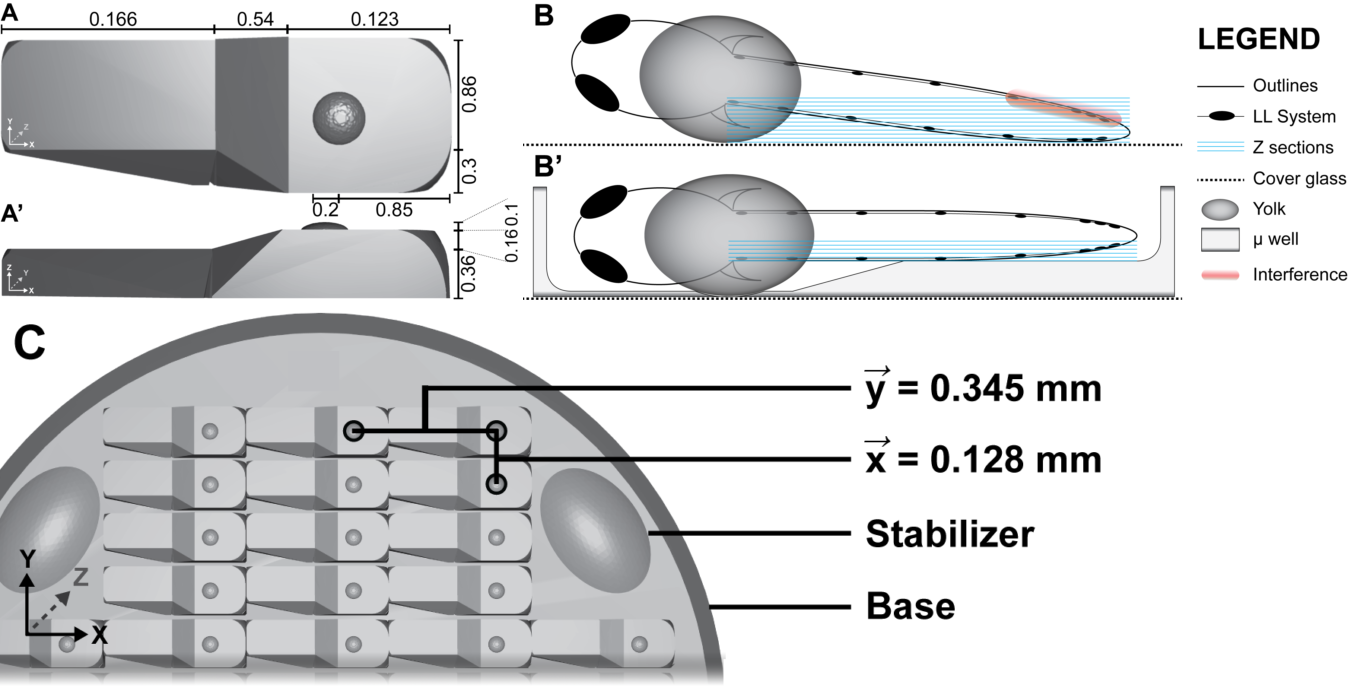
\includegraphics[width=0.8\linewidth]{figure/02-MaMo/Mount/mountmicro} 

}

\caption[Stamp and micro-well properties]{Stamp and \(\mu\)-well properties \textbf{A} single micro well in XY and \textbf{A'} in XZ \textbf{B} mounting without \(\mu\)-well and \textbf{B'} mounting with \(\mu\)-well \textbf{C} elements and dimensions of the stamp.}\label{fig:Mountmicro}
\end{figure}
\hypertarget{protocol}{%
\subsubsection{\texorpdfstring{\textbf{PROTOCOL}}{PROTOCOL}}\label{protocol}}

\hypertarget{preparations}{%
\paragraph{Preparations}\label{preparations}}
\begin{longtable}[]{@{}lccr@{}}
\caption{\label{tab:mounthard} Mounting hardware}\tabularnewline
\toprule
\begin{minipage}[b]{0.25\columnwidth}\raggedright
\textbf{item}\strut
\end{minipage} & \begin{minipage}[b]{0.10\columnwidth}\centering
Company\strut
\end{minipage} & \begin{minipage}[b]{0.45\columnwidth}\centering
Product\strut
\end{minipage} & \begin{minipage}[b]{0.10\columnwidth}\raggedleft
cat.-no.\strut
\end{minipage}\tabularnewline
\midrule
\endfirsthead
\toprule
\begin{minipage}[b]{0.25\columnwidth}\raggedright
\textbf{item}\strut
\end{minipage} & \begin{minipage}[b]{0.10\columnwidth}\centering
Company\strut
\end{minipage} & \begin{minipage}[b]{0.45\columnwidth}\centering
Product\strut
\end{minipage} & \begin{minipage}[b]{0.10\columnwidth}\raggedleft
cat.-no.\strut
\end{minipage}\tabularnewline
\midrule
\endhead
\begin{minipage}[t]{0.25\columnwidth}\raggedright
\(\mu\)-Dish\strut
\end{minipage} & \begin{minipage}[t]{0.10\columnwidth}\centering
ibidi\strut
\end{minipage} & \begin{minipage}[t]{0.45\columnwidth}\centering
20-35 mm polymer, \#1.5, high wall\strut
\end{minipage} & \begin{minipage}[t]{0.10\columnwidth}\raggedleft
81218-200\strut
\end{minipage}\tabularnewline
\begin{minipage}[t]{0.25\columnwidth}\raggedright
3D Mould Stamp\strut
\end{minipage} & \begin{minipage}[t]{0.10\columnwidth}\centering
IBG3D\strut
\end{minipage} & \begin{minipage}[t]{0.45\columnwidth}\centering
20-35 mm\strut
\end{minipage} & \begin{minipage}[t]{0.10\columnwidth}\raggedleft
\strut
\end{minipage}\tabularnewline
\begin{minipage}[t]{0.25\columnwidth}\raggedright
Preparation needles\strut
\end{minipage} & \begin{minipage}[t]{0.10\columnwidth}\centering
VWR\strut
\end{minipage} & \begin{minipage}[t]{0.45\columnwidth}\centering
\strut
\end{minipage} & \begin{minipage}[t]{0.10\columnwidth}\raggedleft
USBE5470\strut
\end{minipage}\tabularnewline
\begin{minipage}[t]{0.25\columnwidth}\raggedright
Glass pipettes\strut
\end{minipage} & \begin{minipage}[t]{0.10\columnwidth}\centering
Roth\strut
\end{minipage} & \begin{minipage}[t]{0.45\columnwidth}\centering
\strut
\end{minipage} & \begin{minipage}[t]{0.10\columnwidth}\raggedleft
4518\strut
\end{minipage}\tabularnewline
\begin{minipage}[t]{0.25\columnwidth}\raggedright
Silicone bulbs\strut
\end{minipage} & \begin{minipage}[t]{0.10\columnwidth}\centering
VWR\strut
\end{minipage} & \begin{minipage}[t]{0.45\columnwidth}\centering
\strut
\end{minipage} & \begin{minipage}[t]{0.10\columnwidth}\raggedleft
612-2327\strut
\end{minipage}\tabularnewline
\begin{minipage}[t]{0.25\columnwidth}\raggedright
Microtubes 2 mL\strut
\end{minipage} & \begin{minipage}[t]{0.10\columnwidth}\centering
Sarstedt\strut
\end{minipage} & \begin{minipage}[t]{0.45\columnwidth}\centering
\strut
\end{minipage} & \begin{minipage}[t]{0.10\columnwidth}\raggedleft
2691\strut
\end{minipage}\tabularnewline
\begin{minipage}[t]{0.25\columnwidth}\raggedright
Heating block\strut
\end{minipage} & \begin{minipage}[t]{0.10\columnwidth}\centering
PeqLab\strut
\end{minipage} & \begin{minipage}[t]{0.45\columnwidth}\centering
\strut
\end{minipage} & \begin{minipage}[t]{0.10\columnwidth}\raggedleft
HX2\strut
\end{minipage}\tabularnewline
\begin{minipage}[t]{0.25\columnwidth}\raggedright
Microwave oven\strut
\end{minipage} & \begin{minipage}[t]{0.10\columnwidth}\centering
Severin\strut
\end{minipage} & \begin{minipage}[t]{0.45\columnwidth}\centering
\strut
\end{minipage} & \begin{minipage}[t]{0.10\columnwidth}\raggedleft
MW7849\strut
\end{minipage}\tabularnewline
\begin{minipage}[t]{0.25\columnwidth}\raggedright
Stereo microscope\strut
\end{minipage} & \begin{minipage}[t]{0.10\columnwidth}\centering
Leica\strut
\end{minipage} & \begin{minipage}[t]{0.45\columnwidth}\centering
\strut
\end{minipage} & \begin{minipage}[t]{0.10\columnwidth}\raggedleft
M165FC\strut
\end{minipage}\tabularnewline
\begin{minipage}[t]{0.25\columnwidth}\raggedright
Transmitted Light Base\strut
\end{minipage} & \begin{minipage}[t]{0.10\columnwidth}\centering
Leica\strut
\end{minipage} & \begin{minipage}[t]{0.45\columnwidth}\centering
\strut
\end{minipage} & \begin{minipage}[t]{0.10\columnwidth}\raggedleft
MDG36\strut
\end{minipage}\tabularnewline
\bottomrule
\end{longtable}
\begin{longtable}[]{@{}lc@{}}
\caption{\label{tab:mountsol} Mounting solutions}\tabularnewline
\toprule
\begin{minipage}[b]{0.39\columnwidth}\raggedright
\textbf{solution}\strut
\end{minipage} & \begin{minipage}[b]{0.55\columnwidth}\centering
Info\strut
\end{minipage}\tabularnewline
\midrule
\endfirsthead
\toprule
\begin{minipage}[b]{0.39\columnwidth}\raggedright
\textbf{solution}\strut
\end{minipage} & \begin{minipage}[b]{0.55\columnwidth}\centering
Info\strut
\end{minipage}\tabularnewline
\midrule
\endhead
\begin{minipage}[t]{0.39\columnwidth}\raggedright
1.0\% (m/V) Agarose / E3\strut
\end{minipage} & \begin{minipage}[t]{0.55\columnwidth}\centering
-\strut
\end{minipage}\tabularnewline
\begin{minipage}[t]{0.39\columnwidth}\raggedright
0.3\% (m/V) LMPA / E3\strut
\end{minipage} & \begin{minipage}[t]{0.55\columnwidth}\centering
incl.~20\% (v/v) 25X TMS for live imaging\strut
\end{minipage}\tabularnewline
\begin{minipage}[t]{0.39\columnwidth}\raggedright
0.5\% (m/V) LMPA / E3\strut
\end{minipage} & \begin{minipage}[t]{0.55\columnwidth}\centering
incl.~20\% (v/v) 25X TMS for live imaging\strut
\end{minipage}\tabularnewline
\bottomrule
\end{longtable}
\hypertarget{preparation}{%
\paragraph{Preparation}\label{preparation}}

First, make sure your stamp is clean of dust or other particles. If necessary clean it with 70\% Ethanol and / or pressured air. Of a 1\% standard Agarose in E3, apply\ldots{}
\begin{itemize}
\tightlist
\item
  600 \(\mu\)L in case of a \(\varnothing\) 35 mm ibidi dish
\item
  2000 \(\mu\)L in case of a \(\varnothing\) 50 mm mattek dish
\end{itemize}
to the glass or polymer surface and place the stamp on it so that it touches the cover. Place it as central as possible. Excessive agarose not needed for the imprint will fill the surrounding area in the dish and stabilize the structure when removing the stamp again.

gently rotate the dish so that excess agarose solution will cover the whole dish.

Wait for \textasciitilde{}45 min., then use a clean preparation needle and slip it through stamp - polymerized agarose interface. Remove the stamp carefully by lifting it and holding the \(\mu\)-Dish in place.


\begin{figure}

{\centering 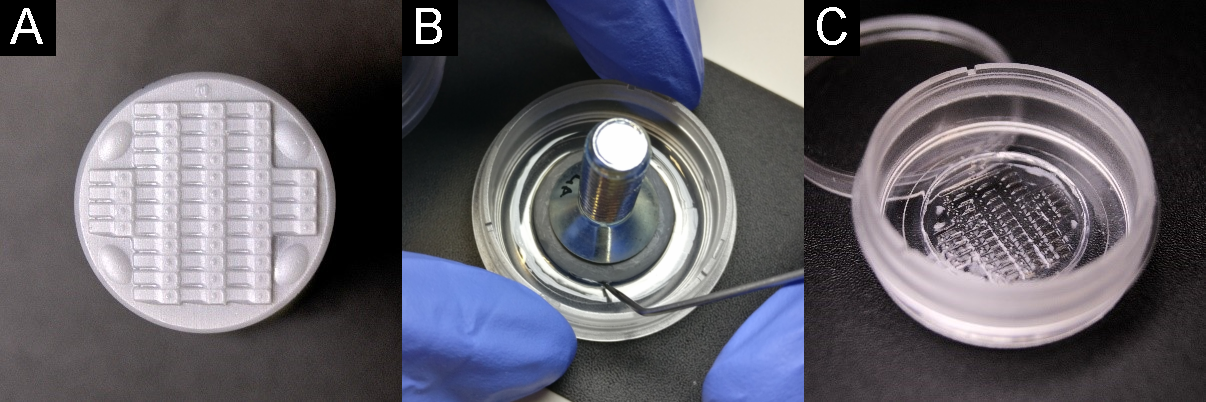
\includegraphics[width=0.6\linewidth]{figure/02-MaMo/Mount/stampprod} 

}

\caption[Stamping procedure]{Stamping procedure \textbf{A} clean stamp surface \textbf{B} preparation of the stamp before lifting \textbf{C} ) ready-for-use agarose imprint.}\label{fig:stampprod}
\end{figure}

\begin{figure}

{\centering 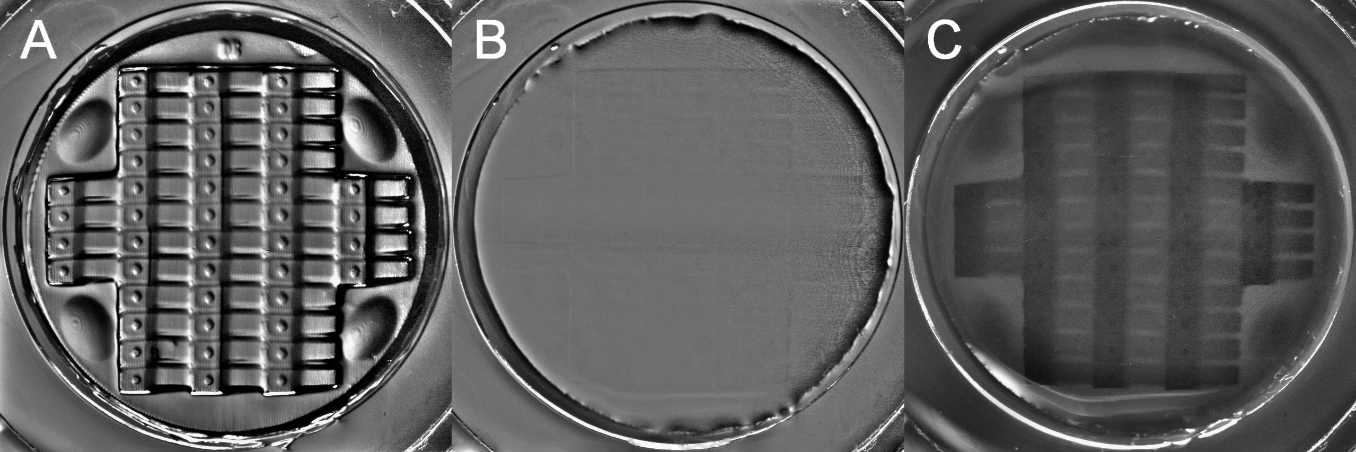
\includegraphics[width=0.6\linewidth]{figure/02-MaMo/Mount/mounting} 

}

\caption[44x mounting stamp]{44x mounting stamp \textbf{A} without LMPA \textbf{B and C} with LMPA, while the latter shows the imprint with light coming from a different angle, making the chambers visible again.}\label{fig:mounting}
\end{figure}

\begin{figure}

{\centering 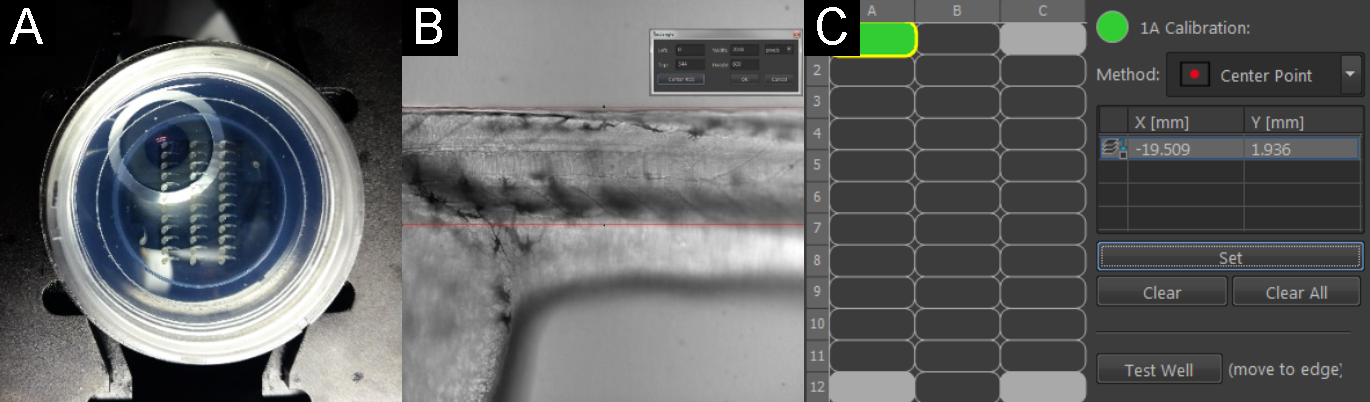
\includegraphics[width=0.6\linewidth]{figure/02-MaMo/Mount/setup} 

}

\caption[Imaging setup]{Imaging setup \textbf{A} Positioning of the \(\mu\)-well \textbf{B} Alignment in Brightfield and \textbf{C} Definition of a custom well plate.}\label{fig:setup}
\end{figure}
\hypertarget{comp-met}{%
\subsection{Computational Methods}\label{comp-met}}

\hypertarget{CNN}{%
\subsubsection{Rosette Detection}\label{CNN}}

The method used for rosette detection is based on a convolutional neuronal network (CNN) and is similar method to what was used before by Ernst \emph{et al.}(2012)(\emph{29}, \emph{41}) for the description of the \emph{shroom3} morpholino injected phenotype. Since the former method was technically deprecated and since we had new data to detect rosettes, we updated the former method to a state of the art CNN using Caffe(\emph{52}) as a backend. The training was done by our partners at the institute for informatics, Albert-Ludwigs-University Freiburg.

The CNN was trained on 17 wildtype DMSO control and SU5402 treated (Fgf signaling depleted embryos which do not form rosettes(\emph{27})) embryos each. In order togive the network something to learn, the data had to be labeled manually, which was done in imagej by placing multipoint rois at the center of the rosettes. The data was then further permutated to artificially increase the amount of training data and make the detection more robust against different kinds of input. Further parameters about the training data is listed in Table \ref{tab:CNNtraining}. One example for each is shown in figure \ref{fig:CNNtrain}.


\begin{figure}

{\centering 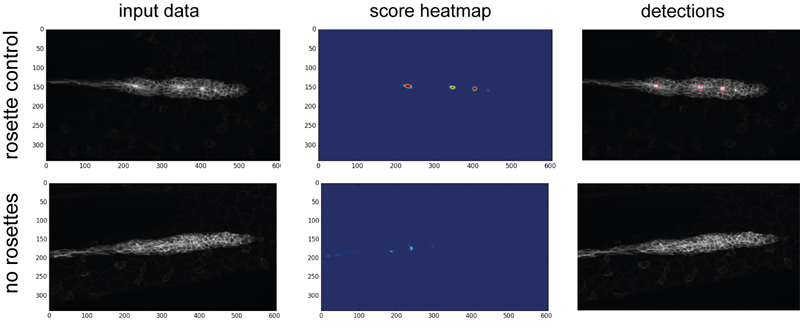
\includegraphics[width=0.75\linewidth]{figure/02-MaMo/CNN/CNNtrain} 

}

\caption[Example for rosette detection on the training data]{Example for rosette detection on the training data. \textbf{left} Maximum Z-projected input data. \textbf{middle} heatmap of scores. blue indicates a low score, red a high one. \textbf{right} score map projected onto the input data.}\label{fig:CNNtrain}
\end{figure}
\noindent The main advantages for using a neural network in a task like this are\ldots{}
\begin{enumerate}
\def\labelenumi{\arabic{enumi}.}
\tightlist
\item
  Objectivity
  \begin{itemize}
  \tightlist
  \item
    Unlike the human brain, one a CNN is trained it is static and does not keep on learning. This makes it possible to have an unbiased quantification of rosette counts.
  \end{itemize}
\item
  Degree of rosette registration
  \begin{itemize}
  \tightlist
  \item
    The output data are continous rational numbers (\(\mathbb{Q}\)) instead of integers (\(\mathbb{Z}\)) which does not only tell if a rosette is there fore not, but also for `how much' (50-100\%) it is there.
  \end{itemize}
\item
  Training is done relatively quick
\end{enumerate}
\begin{longtable}[]{@{}llllllll@{}}
\caption{\label{tab:CNNtraining} CNN training data}\tabularnewline
\toprule
& compound & conc. & nm & intensity & exposure & z-planes & magnification\tabularnewline
\midrule
\endfirsthead
\toprule
& compound & conc. & nm & intensity & exposure & z-planes & magnification\tabularnewline
\midrule
\endhead
Rosette control & DMSO & 1\% & 488 & 100\% & 100 ms & \textasciitilde{}70 & 40X\tabularnewline
SU5402 treated & SU5402 & 10 \(\mu\)M & 488 & 100\% & 100 ms & \textasciitilde{}70 & 40X\tabularnewline
\bottomrule
\end{longtable}
\hypertarget{prolif}{%
\subsubsection{Proliferation Analysis}\label{prolif}}

The basic principle is based on work done by Laguerre \emph{et al.}, 2009(\emph{23}).

\noindent For manual tracking of mitotic events `MTrackJ'(\emph{53}) was used
\begin{itemize}
\tightlist
\item
  Mitotic events were tracked in the pLLP exclusively from Prometa- / Meta-phase till Ana- / Telo-phase
\item
  After tracking, the track file was saved and measured
\item
  `Tracks' and `Points' data was saved as `.txt' files (tab seperated)
\end{itemize}
\noindent Figure \ref{fig:mitodatapoints} shows an exemplary track for the data analyzed.


\begin{figure}

{\centering 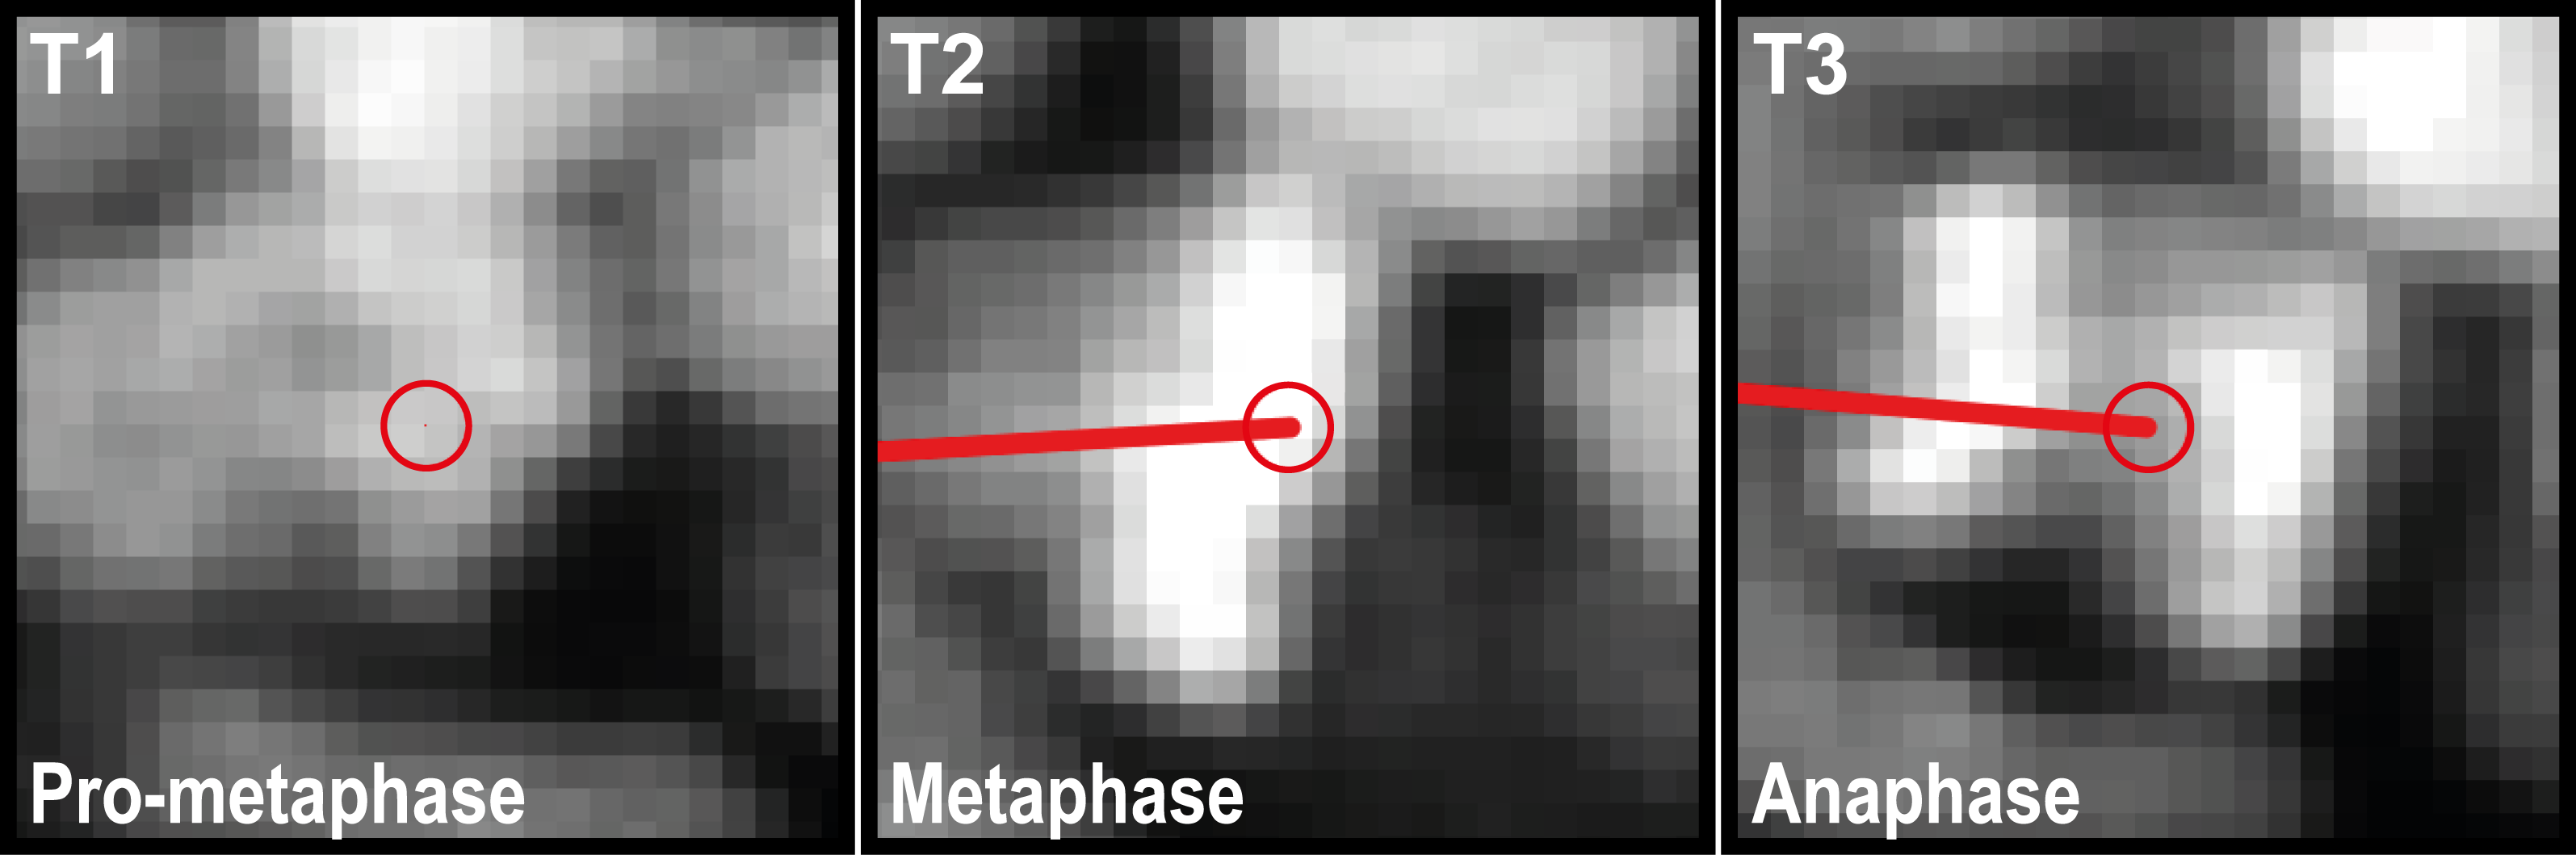
\includegraphics[width=0.5\linewidth]{figure/02-MaMo/Prol/Prolif} 

}

\caption{Tracking of mitotic events}\label{fig:mitodatapoints}
\end{figure}
\hypertarget{ACI}{%
\subsubsection{Apical Index}\label{ACI}}

The earliest attempt found for indexing AC can be found in a study published by Lee \emph{et al}(\emph{54}) where they were interested in the `apical index' (A.I.) of bottle cells during \emph{X.laevis} gastrulation(figure \ref{fig:ACLee}).


\begin{figure}

{\centering 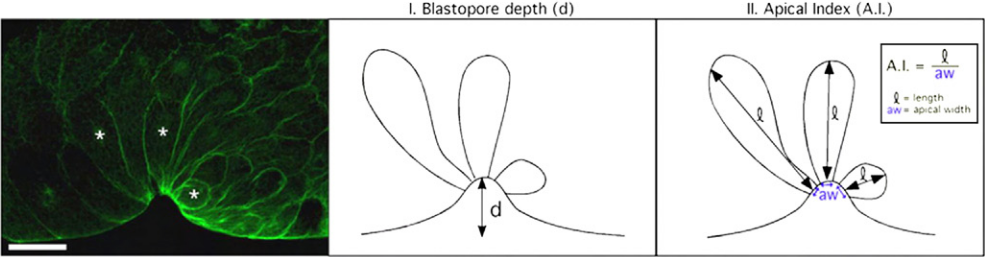
\includegraphics[width=0.75\linewidth]{figure/02-MaMo/ACI/Jen_yi_Lee} 

}

\caption{A.I. of \emph{X.leavis} bottle cells.}\label{fig:ACLee}
\end{figure}
\noindent Another example for measuring AC is the apical \emph{constriction} index (ACI, figure \ref{fig:ACHard}) for the cells of the \emph{D.rerio} lateral line primordium (PLLp), which can be found in a study from 2012 where it was shown that Fgfr-Ras-MAPK signaling is required for AC and Rock2a localization6 (\emph{55}, \emph{56}).


\begin{figure}

{\centering 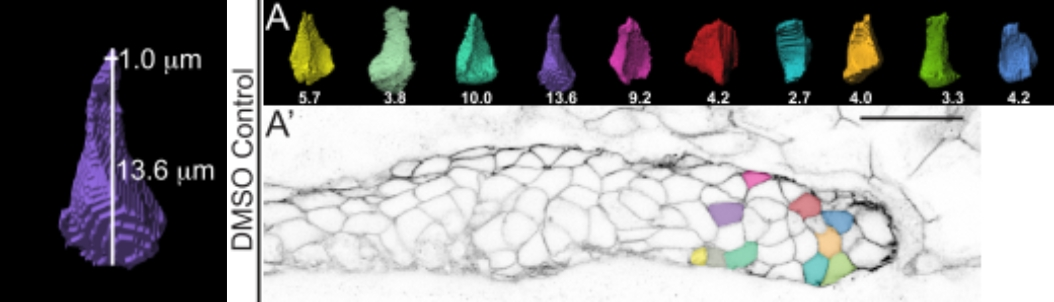
\includegraphics[width=0.75\linewidth]{figure/02-MaMo/ACI/Harding} 

}

\caption[Apical constriction index]{Apical constriction index. \textbf{A} 3D reconstructed cells of a CLCLNA control primordium and \textbf{B} of a primordium deficient of Fgf signaling.}\label{fig:ACHard}
\end{figure}
\noindent In both cases, the measurements for the A.I.(\emph{54}) or ACI(\emph{56}) does not differ and describes the ratio for lateral height over apical width \ref{fig:ACICells}.

\[\mathbf{ACI} = \frac{lateral\;height\;[\mu m]}{apical\;width\;[\mu m]}\]

\noindent While trying to reproduce these results we found two principal weaknesses of applying this ratio to the cells of the PLLp. First, it does not respect the independence of lateral height to AC. Second, it does not differentiate between \emph{anterio-posterior} (AP) and \emph{dorso-ventral} (DV) tissue polarization. Third, it is really more an A.I. than a constriction index.

\hypertarget{rationale}{%
\paragraph{Rationale}\label{rationale}}

\hypertarget{ACI-param}{%
\subparagraph{Parameter definition}\label{ACI-param}}

To obtain a precise and biologically meaningful quantity for AC, first a couple of definitions have to be made.
\begin{enumerate}
\def\labelenumi{\arabic{enumi}.}
\tightlist
\item
  AC is independent of orientation and polarization
  \begin{itemize}
  \tightlist
  \item
    Cells can be polarized along the AP axis
  \item
    Cells can also be polarized along the DV axis
  \end{itemize}
\item
  AC is independent of lateral height
  \begin{itemize}
  \tightlist
  \item
    Lateral height can be described as the distance of the two farthest points on the surface area of a cell
  \item
    Two cells with different lateral heights can be equally apically constricted
  \end{itemize}
\item
  AC is independent of cell size
  \begin{itemize}
  \tightlist
  \item
    The size of a cell is its volume
  \item
    Two cells of different volume can be equally apically constricted
  \end{itemize}
\end{enumerate}
\hypertarget{ACI-lat}{%
\subparagraph{Adaption for variation in lateral height}\label{ACI-lat}}

To test different ACI conditions, an apically constricted cell can be approximated by modeling a tetrahedron. For example, shrinking or enlarging a cell symmetrically should not affect the ACI. As described by Harding(2014)(\emph{56}), the \emph{apical width} of a cell is measured first by manual 3-D object reconstruction, second manual re-orientation, and third by going 1 \(\mu\)m from the apical tip into the cell (from now on referred to as \(\Delta\)ap, \ref{fig:ACICells}B). Finally, \emph{apical width} is the total width of the 2-D object.

If \(\Delta\)ap is a constant, the ACI in a symmetrically enlarged cell increases from e.g.~15 to 23, since \emph{apical width} stays the same but lateral height increases. On the contrary, if \(\Delta\)ap is adjusted relative to a cells lateral height, e.g.~by percentage, the ACI in a symmetrically enlarged cell stays the same \ref{fig:ACICells}


\begin{figure}

{\centering 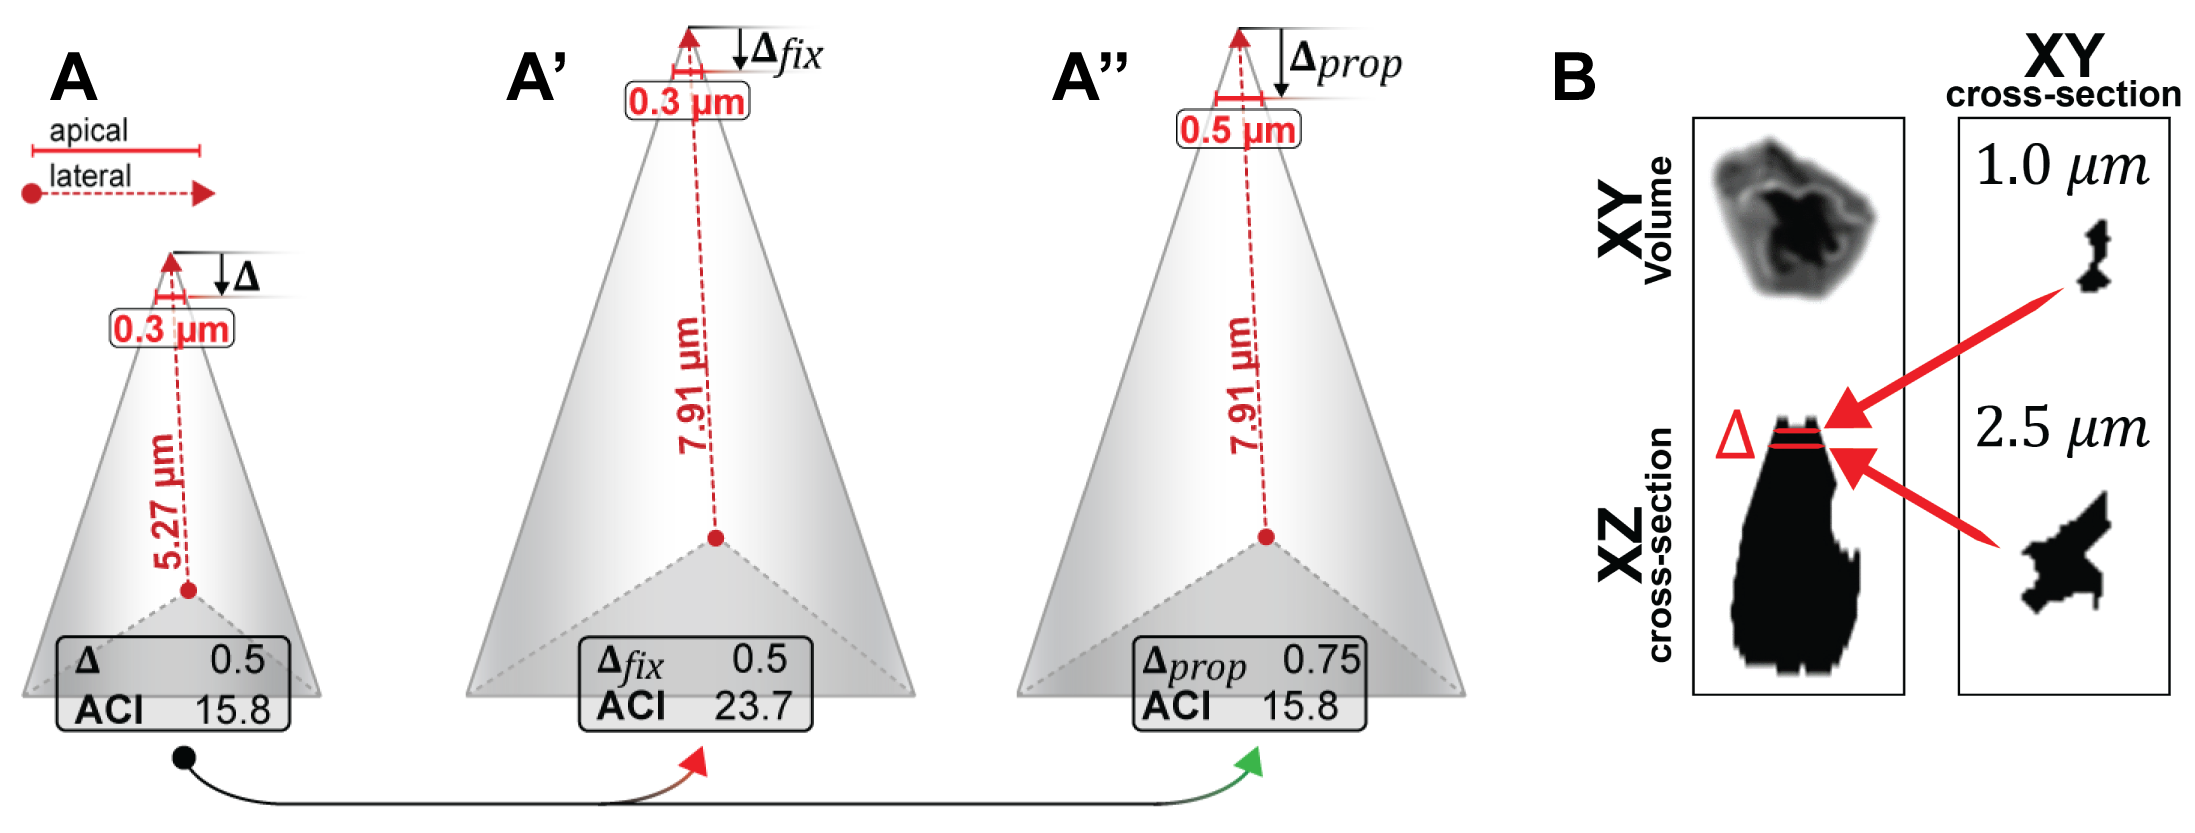
\includegraphics[width=0.75\linewidth]{figures/summary/aci_fig-01} 

}

\caption[ACI Cell Models]{ACI model \textbf{A-A''} ACI Cell Models. A' and A'' show cells that are symmetrically increased versions of A. While in A', constant delta was used, in A'' delta was adjusted relative to the lateral height. \textbf{B} Illustrating delta ap. (left) apically constricted cells volume rendered in XY (top) and as a lateral cross-section in X-Z (bottom). (right) 2D area as seen at delta ap of 1 or 2.5 \(\mu\)m.}\label{fig:ACICells}
\end{figure}
Therefore the measurement for apical width has to be relative to lateral height.

\[\mathbf{ACI} = \frac{lateral\;height\;[\mu m]}{relative\;apical\;width\;[\mu m]}\]

\hypertarget{ACI-pol}{%
\subparagraph{Adaption for tissue polarization}\label{ACI-pol}}

Organs develop in a 3-D space and are polarized along each axis. AC usually describes a 2-D morphogenetic movement towards a center along the X-Y axes. However, the contraction movements along X and Y might be independent of one another. This could mean that they happen at different speeds, or that one is absent. As a result, the tissue would look less radially \ref{fig:cellpol} constricted, but more constricted against a line. In order to separate those two AC dimensions, the ACI can be calculated for the \emph{anterio-posterior} and for the \emph{dorso-ventral} axis \ref{fig:cellpol}.


\begin{figure}

{\centering 
\includegraphics[width=0.75\linewidth]{figure/02-MaMo/ACI/ACI_Cells_pol} 

}

\caption[Schematic anisotropic AC]{Schematic AC along the A-P and D-V axis. \textbf{A} shows a A-P and D-V constricted cluster of cells. \textbf{B} shows a D-V constricted cluster of cells.}\label{fig:cellpol}
\end{figure}
\noindent By fitting an ellipsoid to the volume area taken at \(\mathrm{\Delta}\)ap, one will obtain the following parameters.
\begin{enumerate}
\def\labelenumi{\arabic{enumi}.}
\tightlist
\item
  Length of Major axis (figure \ref{fig:ellipse})
  \begin{itemize}
  \tightlist
  \item
    constituting \emph{apical width}
  \end{itemize}
\item
  Length of Minor axis (figure \ref{fig:ellipse})
  \begin{itemize}
  \tightlist
  \item
    constituting \emph{apical height}
  \end{itemize}
\item
  Angle of Major from 0\(^\circ\) (figure \ref{fig:ellipse})
  \begin{itemize}
  \tightlist
  \item
    indicative for orientation of \emph{lateral height}
  \end{itemize}
\end{enumerate}

\begin{figure}

{\centering 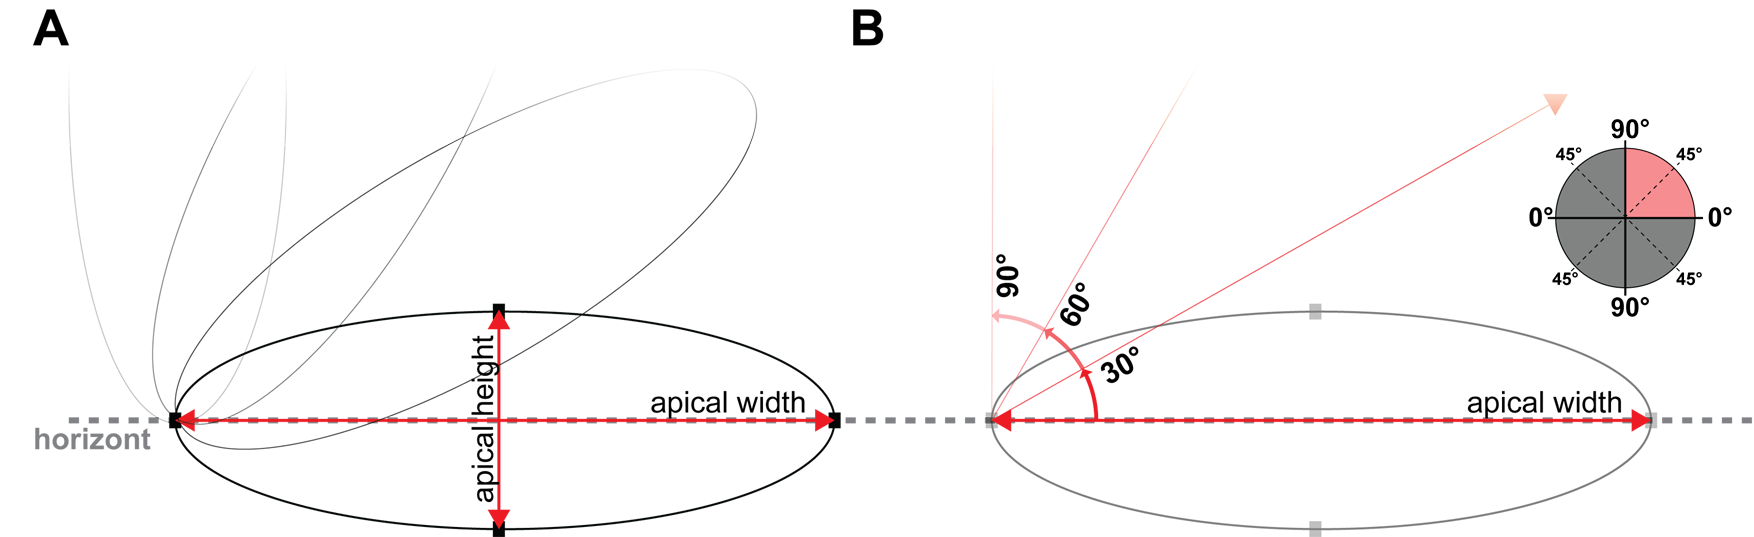
\includegraphics[width=0.75\linewidth]{figure/02-MaMo/ACI/ellipse} 

}

\caption[Scheme of ellipsoid measures]{Scheme of ellipsoid measures. \textbf{A} shows the major axis as apical width and the minor axis as apical height. \textbf{B} shows the angular displacement from the horizon in steps of 30\(^\circ\).}\label{fig:ellipse}
\end{figure}
The two dimensions of AC indices can therefore be described as the following ratios\ldots{}

\[\mathbf{ACI_{Major}} = \frac{lateral\;height\;[\mu m]}{Major\;axis\;[\mu m]}\]
\[\mathbf{ACI_{Minor}} = \frac{lateral\;height\;[\mu m]}{Minor\;axis\;[\mu m]}\]
\[\mathbf{Angle_{Major}} = \measuredangle = \mathrm{\Delta}\;from\;horizont\;[0-90^\circ]\]

\hypertarget{ACI-Dis}{%
\paragraph{Measurements}\label{ACI-Dis}}

\hypertarget{ACI-singlecell}{%
\subparagraph{Single Cell measurements}\label{ACI-singlecell}}

Each geometric object has a centroid coordinate in X and Y (and Z) which is represented as the mean of all X or Y coordinates within the object. Here, the centroid coordinates in X and Y are used to plot the cells as points in the X-Y plane. Additionally, each point is colored for the ACI value (high values are blue-violet, middle values are green, low values are yellow-red).


\begin{figure}

{\centering 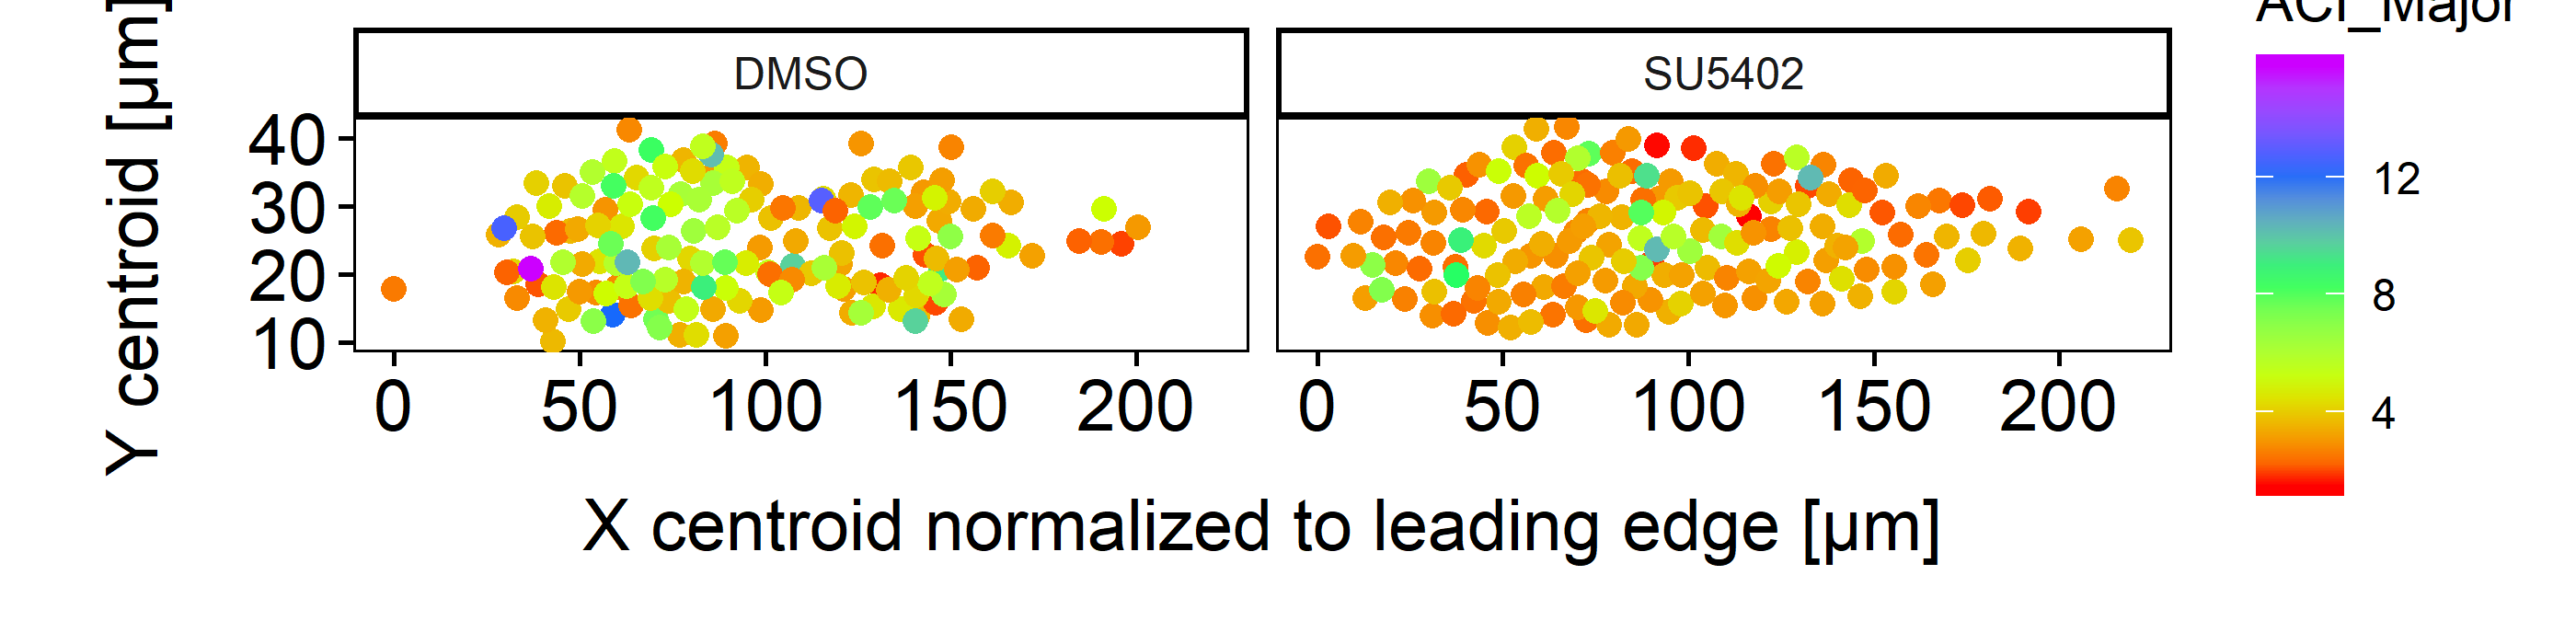
\includegraphics[width=0.85\linewidth]{thesis_files/figure-latex/ACIMajor-1} 

}

\caption{ACI\textsubscript{Major} single cell measurements}\label{fig:ACIMajor}
\end{figure}

\begin{figure}

{\centering 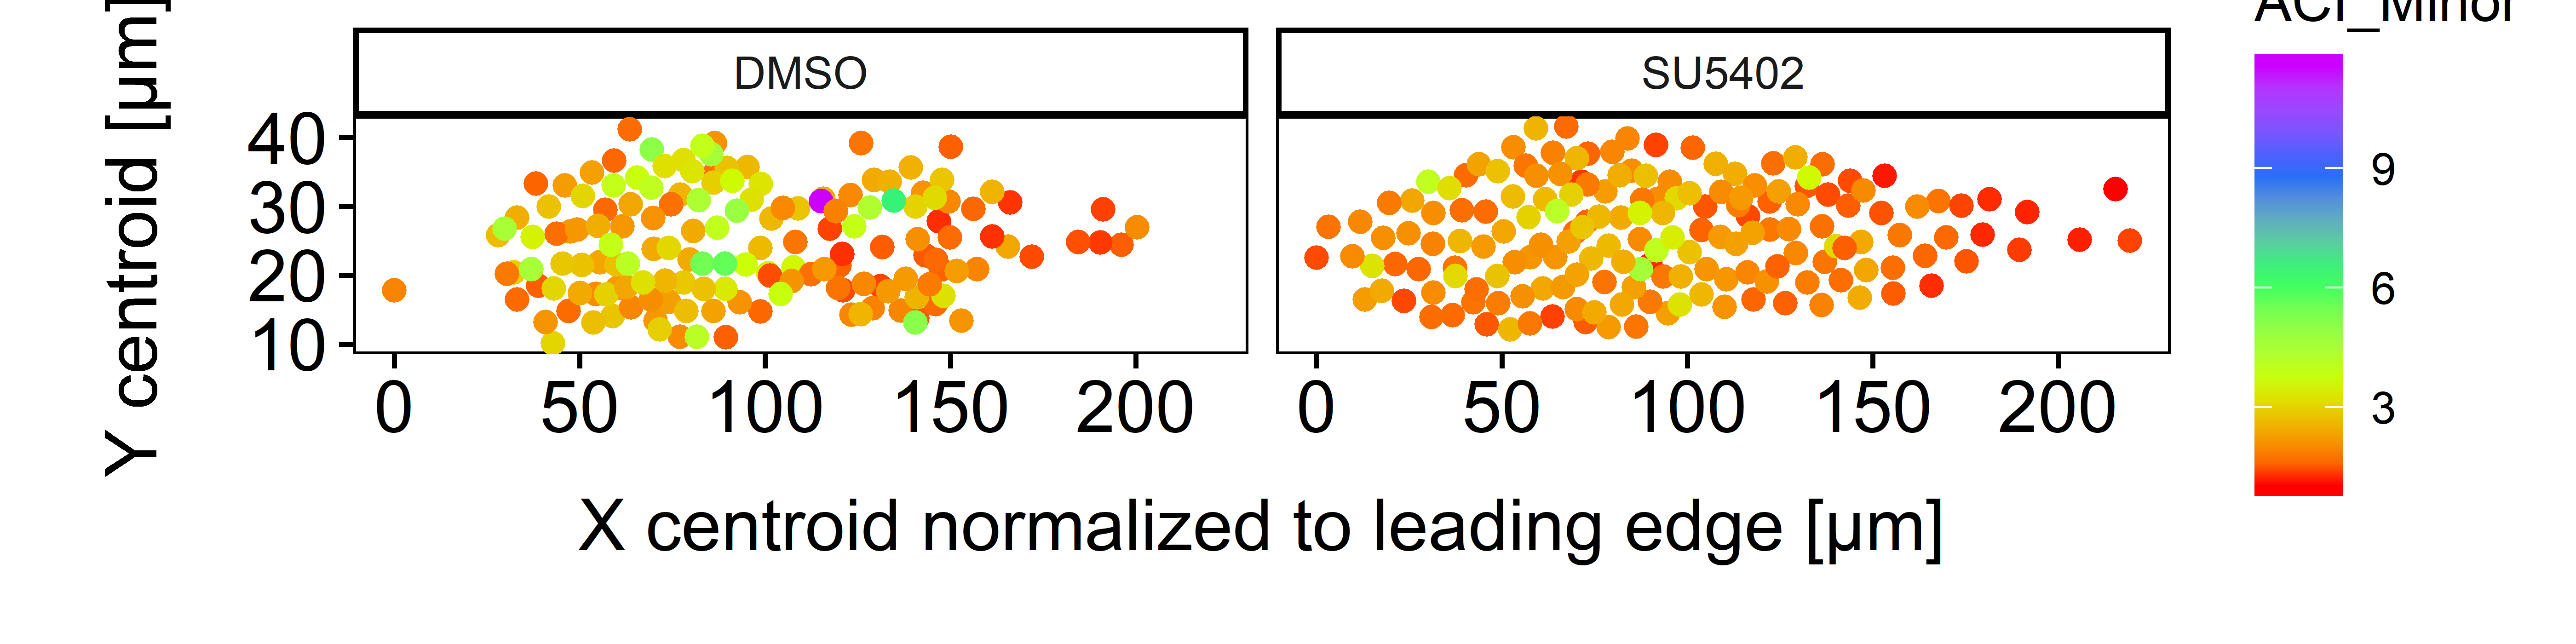
\includegraphics[width=0.85\linewidth]{thesis_files/figure-latex/ACIMinor-1} 

}

\caption{ACI\textsubscript{Minor} single cell measurements}\label{fig:ACIMinor}
\end{figure}
Harding(2013)(\emph{56}) were using a constant \(\mathrm{\Delta}\)ap to measure the apical width, which we have shown to be incorrect in certain cases. In their study they found that certain mean ACI values in the DMSO go as high as 15, which might be related to this \ref{fig:ACICells}.
By measuring apical width at a relative \(\mathrm{\Delta}\)ap the mean values for ACI\textsubscript{Major} are at 4.7 for the DMSO control and 3.6 for the SU5402 treated condition, which seems to somewhat correlate with their findings\ref{fig:HardingACI}. .

However overall our results indicate that the AC difference is not as strong, at least if all the cells of the PLLp are taken into account.


\begin{figure}

{\centering 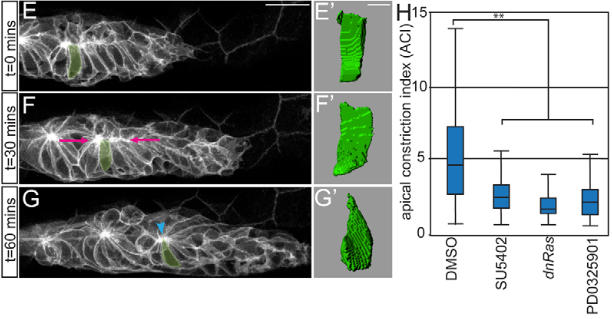
\includegraphics[width=0.6\linewidth]{figure/02-MaMo/GrTr/HardingACI} 

}

\caption[Published ACI]{\textbf{E-G} 3-D reconstructions of the highlighted cell. \textbf{H} ACIs for embryos treated with DMSO, SU5402, PD0325901 or following induction of hsp70:dn-Ras. (n=180 cells / N = 6 embryos).}\label{fig:HardingACI}
\end{figure}
\hypertarget{ACI-Angledens}{%
\subparagraph{Angle densities}\label{ACI-Angledens}}

To check whether there is a bias in orientation of the apical width, the angle measurements \ref{fig:ellipse} can be shown as a function of density along X. Here, a binwidth of 2.5 and a grouping factor to color the two conditions `DMSO' and `SU5402' was used.

\noindent Interestingly the results indicate that there is less of a difference for the Major\textsubscript{Angle} at angles bigger than 15-20°. This would mean that the \emph{apical width} in SU5402 treated embryos is more strongly oriented along the horizontal \emph{antero-posterior} axis.


\begin{figure}

{\centering 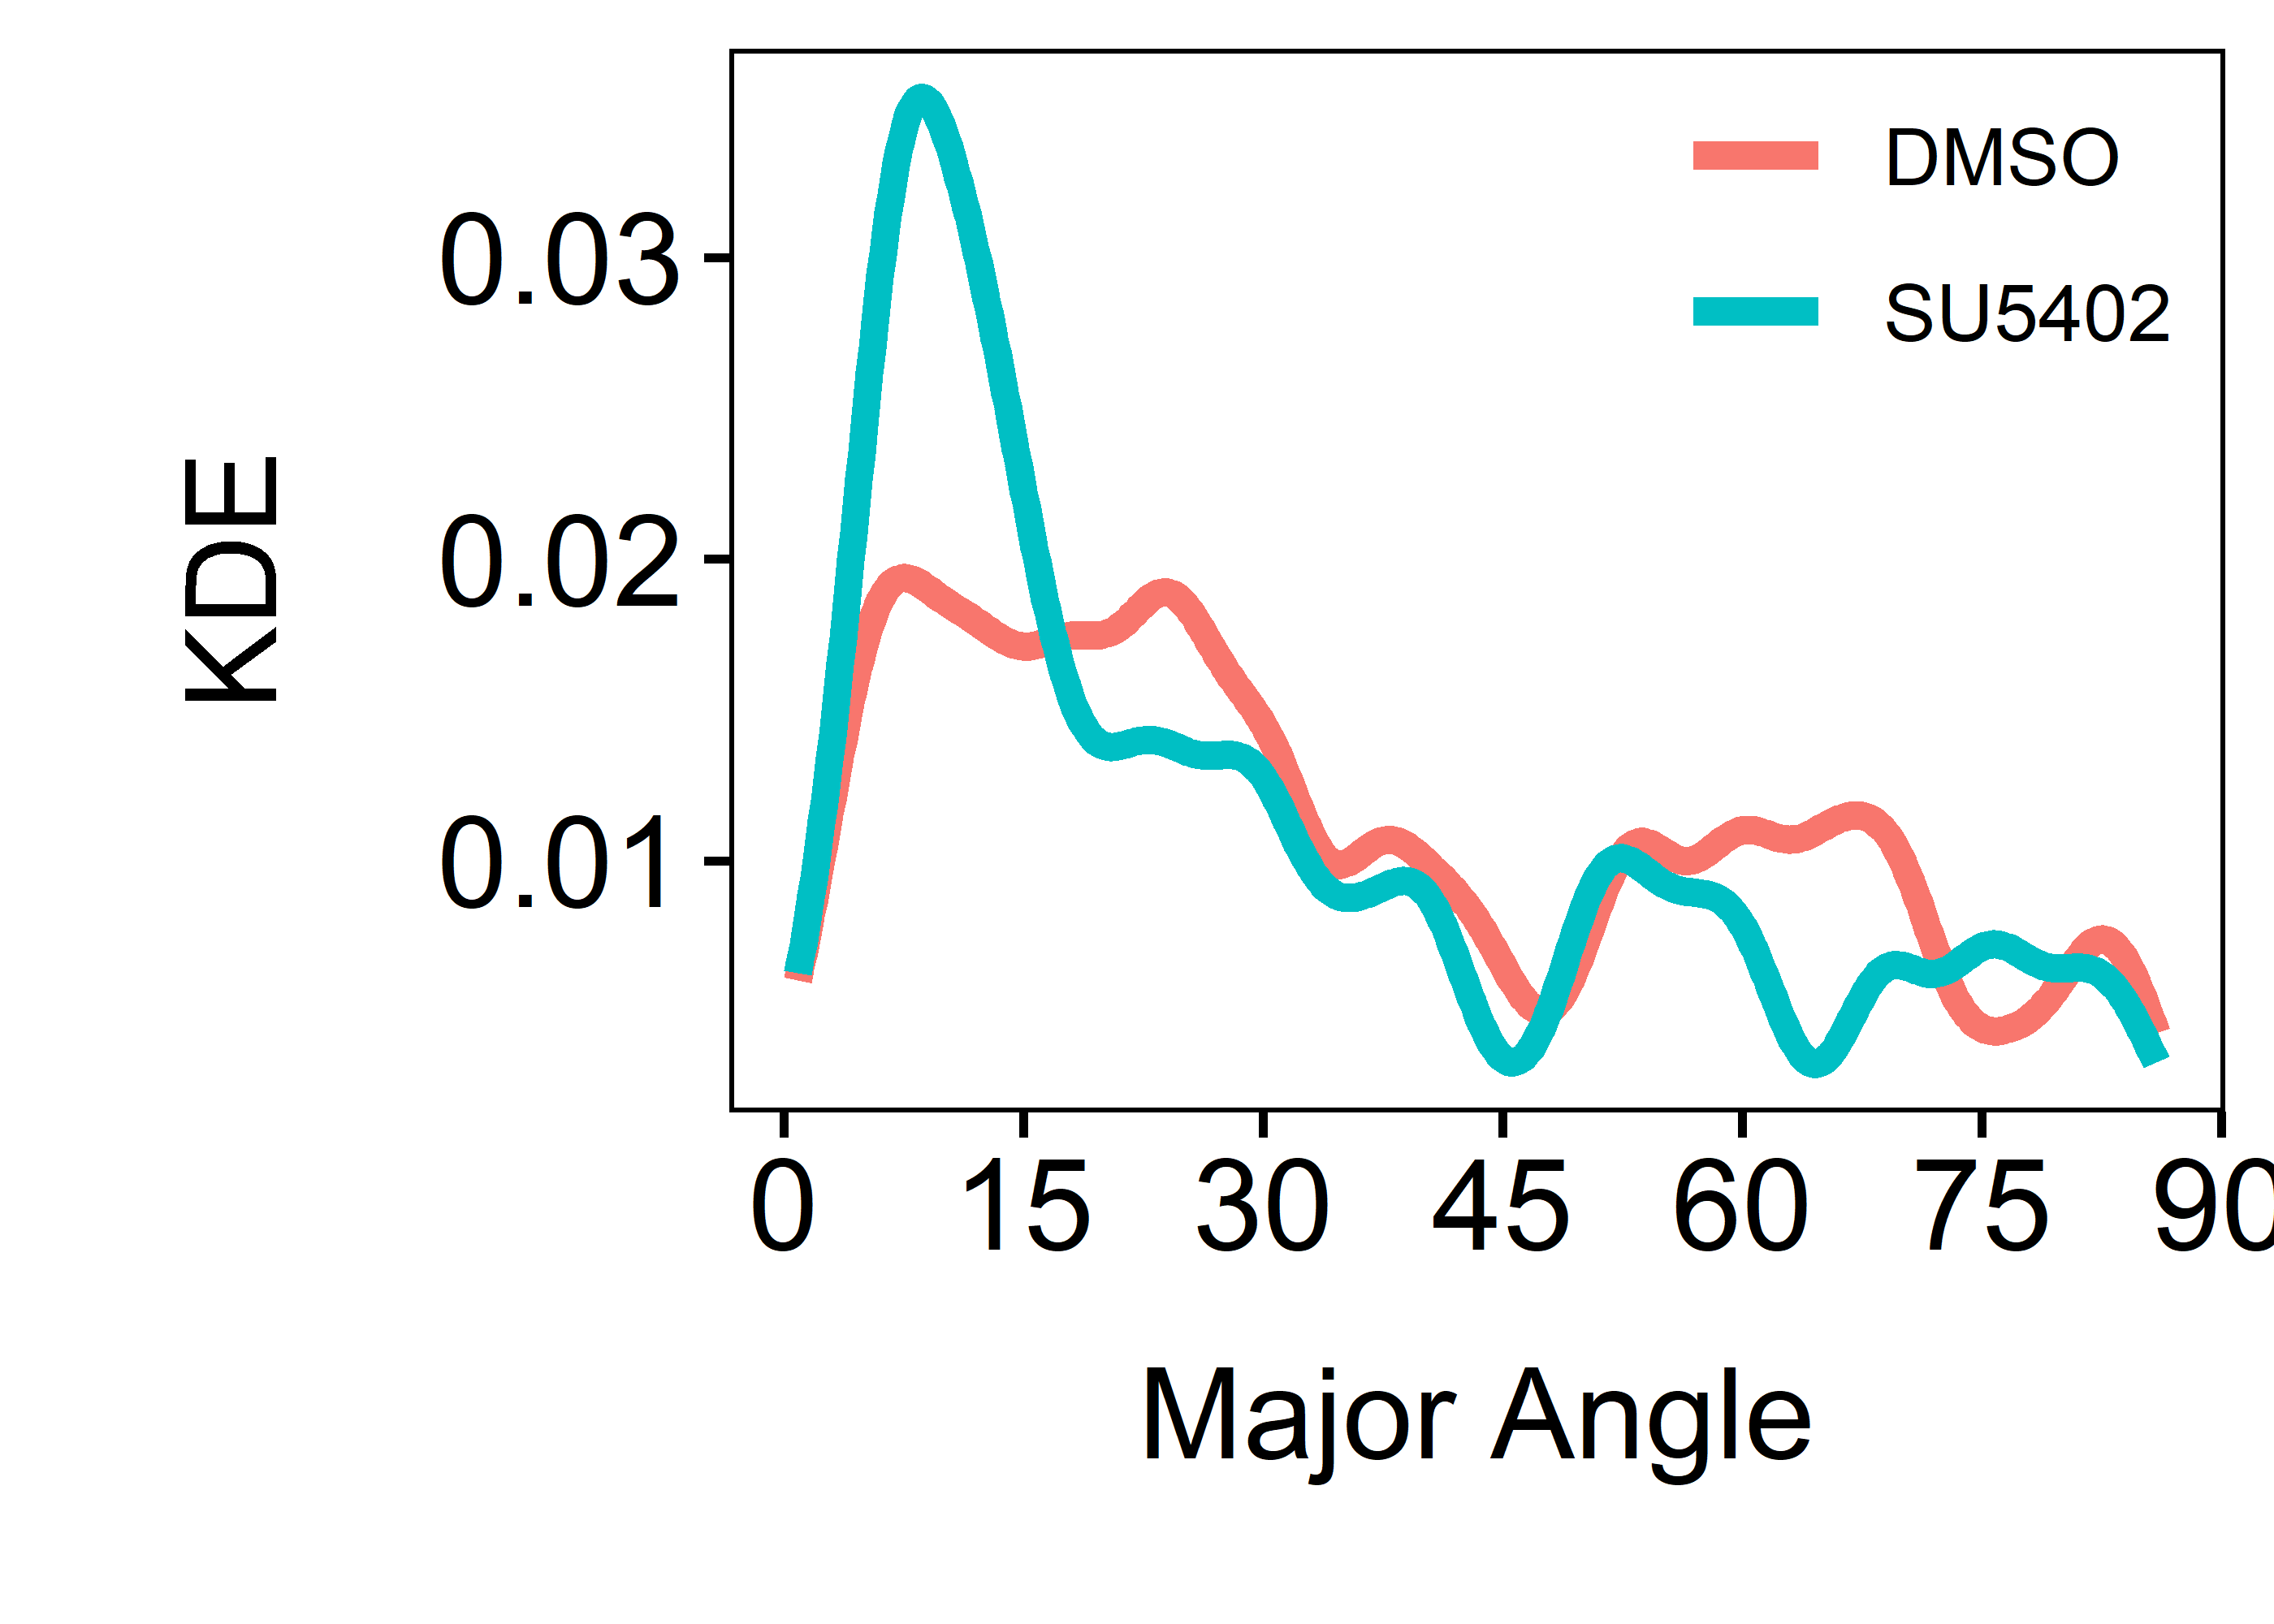
\includegraphics[width=0.4\linewidth]{thesis_files/figure-latex/angledens-1} 

}

\caption{Major\textsubscript{Angle} density}\label{fig:angledens}
\end{figure}
\hypertarget{ACI-mag}{%
\subparagraph{ACI magnitude at different Angles}\label{ACI-mag}}

Now, to get an idea of the magnitude ACI\textsubscript{Major} and ACI\textsubscript{Minor} have at each angle, each can be shown as a function of the Major\textsubscript{Angle} over ACI (while Major\textsubscript{Angle} is the same for both ACIs). Again, the grouping factor `GT' was used to color the two conditions `DMSO' and `SU5402'.

\noindent Since AC is a 3-D morphogenetic process and since cells in a wild type PLLp are mostly radially organized, it does make sense to try to look at AC from more than just one perspective. Here we propose to separate the ACI into an \emph{antero-posterior} and a \emph{dorso-ventral} dimension.
\begin{enumerate}
\def\labelenumi{\arabic{enumi}.}
\item
  Interestingly there does not seem to be much of a difference in ACI\textsubscript{Minor}, which can also be shown by the mean values which are at 2.6 for the DMSO control and at 2.1 for the SU5402 treated condition. This indicates that there is no significant difference in contraction along the \emph{dorso-ventral} axis.
\item
  For the ACI\textsubscript{Major} the base constriction for both, DMSO and SU5402 is at around 3.6, however there is a peak at around 40-60° in the DMSO control where cells are most constricted having a maximum ACI at 15.8. This indicates that cells coming from 35.7° are most constricted in the \emph{anterior-posterior} axis.
\end{enumerate}

\begin{figure}

{\centering 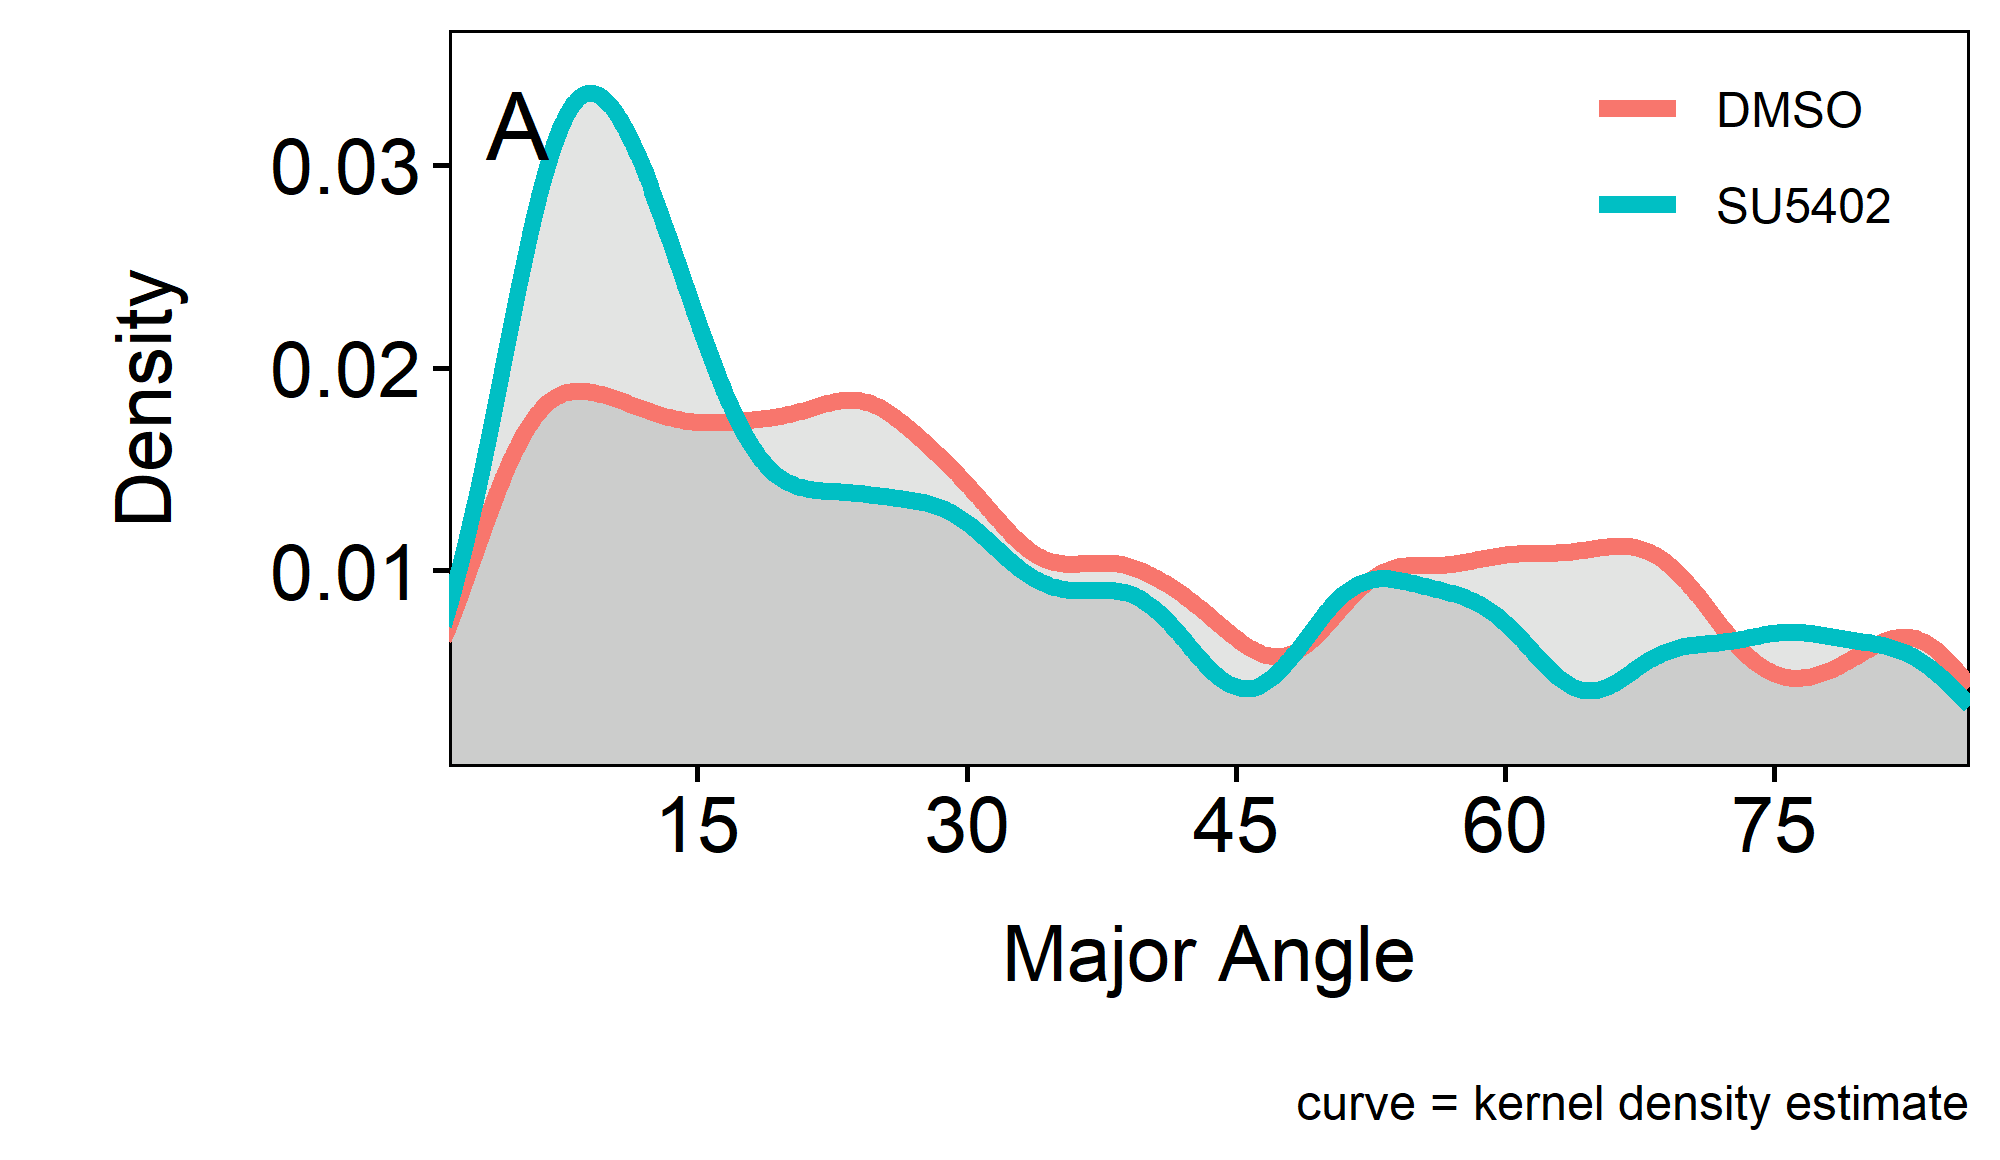
\includegraphics[width=0.6\linewidth]{thesis_files/figure-latex/angletoACI-1} 

}

\caption{ACI\textsubscript{Major} / ACI\textsubscript{Minor} over Major\textsubscript{Angle}}\label{fig:angletoACI}
\end{figure}
\hypertarget{summary-3}{%
\paragraph{Summary}\label{summary-3}}

In summary our results suggest that there is no significant difference either in the exact \emph{anterior-posterior} axis (at 0°), nor in the exact \emph{dorso-ventral} axis (at 90\(^\circ\)) between a DMSO control and a SU5402 treated embryo, but mostly in an angle in between.

\hypertarget{mat-datasets}{%
\section{Image Data Sets}\label{mat-datasets}}

\hypertarget{cc-data}{%
\subsection{Cell-Cluster}\label{cc-data}}
\begin{longtable}[]{@{}ll@{}}
\caption{\label{tab:ccdata} Cell Cluster dataset}\tabularnewline
\toprule
\endhead
\begin{minipage}[t]{0.21\columnwidth}\raggedright
\textbf{Crossings}\strut
\end{minipage} & \begin{minipage}[t]{0.73\columnwidth}\raggedright
\strut
\end{minipage}\tabularnewline
\begin{minipage}[t]{0.21\columnwidth}\raggedright
Pairs\strut
\end{minipage} & \begin{minipage}[t]{0.73\columnwidth}\raggedright
4\strut
\end{minipage}\tabularnewline
\begin{minipage}[t]{0.21\columnwidth}\raggedright
Transgenes\strut
\end{minipage} & \begin{minipage}[t]{0.73\columnwidth}\raggedright
\emph{cldnb:lyn-gfp} +/?\strut
\end{minipage}\tabularnewline
\begin{minipage}[t]{0.21\columnwidth}\raggedright
Mutation\strut
\end{minipage} & \begin{minipage}[t]{0.73\columnwidth}\raggedright
\emph{shroom3}\strut
\end{minipage}\tabularnewline
\begin{minipage}[t]{0.21\columnwidth}\raggedright
Staging\strut
\end{minipage} & \begin{minipage}[t]{0.73\columnwidth}\raggedright
60 min.\strut
\end{minipage}\tabularnewline
\begin{minipage}[t]{0.21\columnwidth}\raggedright
\textbf{Mounting}\strut
\end{minipage} & \begin{minipage}[t]{0.73\columnwidth}\raggedright
\strut
\end{minipage}\tabularnewline
\begin{minipage}[t]{0.21\columnwidth}\raggedright
Fixation\strut
\end{minipage} & \begin{minipage}[t]{0.73\columnwidth}\raggedright
4\% PFA o.N.\strut
\end{minipage}\tabularnewline
\begin{minipage}[t]{0.21\columnwidth}\raggedright
agarose\strut
\end{minipage} & \begin{minipage}[t]{0.73\columnwidth}\raggedright
1\% LMPA\strut
\end{minipage}\tabularnewline
\begin{minipage}[t]{0.21\columnwidth}\raggedright
\textbf{Imaging}\strut
\end{minipage} & \begin{minipage}[t]{0.73\columnwidth}\raggedright
\strut
\end{minipage}\tabularnewline
\begin{minipage}[t]{0.21\columnwidth}\raggedright
Magnification\strut
\end{minipage} & \begin{minipage}[t]{0.73\columnwidth}\raggedright
25X objective\strut
\end{minipage}\tabularnewline
\begin{minipage}[t]{0.21\columnwidth}\raggedright
Channels\strut
\end{minipage} & \begin{minipage}[t]{0.73\columnwidth}\raggedright
488 nm\strut
\end{minipage}\tabularnewline
\begin{minipage}[t]{0.21\columnwidth}\raggedright
Z-Stack\strut
\end{minipage} & \begin{minipage}[t]{0.73\columnwidth}\raggedright
2.5 \(\mu\)m Z-spacing; 110 \(\mu\)m stack size; 12*X large image\strut
\end{minipage}\tabularnewline
\begin{minipage}[t]{0.21\columnwidth}\raggedright
\textbf{Processing}\strut
\end{minipage} & \begin{minipage}[t]{0.73\columnwidth}\raggedright
\strut
\end{minipage}\tabularnewline
\begin{minipage}[t]{0.21\columnwidth}\raggedright
Projection\strut
\end{minipage} & \begin{minipage}[t]{0.73\columnwidth}\raggedright
Maximum intensity\strut
\end{minipage}\tabularnewline
\begin{minipage}[t]{0.21\columnwidth}\raggedright
Transformations\strut
\end{minipage} & \begin{minipage}[t]{0.73\columnwidth}\raggedright
Rotation and cropping in XY\strut
\end{minipage}\tabularnewline
\bottomrule
\end{longtable}
\hypertarget{aci-data}{%
\subsection{Apical Index}\label{aci-data}}
\begin{longtable}[]{@{}ll@{}}
\caption{\label{tab:acidata} AI dataset}\tabularnewline
\toprule
\endhead
\begin{minipage}[t]{0.21\columnwidth}\raggedright
\textbf{Crossings}\strut
\end{minipage} & \begin{minipage}[t]{0.73\columnwidth}\raggedright
\strut
\end{minipage}\tabularnewline
\begin{minipage}[t]{0.21\columnwidth}\raggedright
Pairs\strut
\end{minipage} & \begin{minipage}[t]{0.73\columnwidth}\raggedright
4\strut
\end{minipage}\tabularnewline
\begin{minipage}[t]{0.21\columnwidth}\raggedright
Transgenes\strut
\end{minipage} & \begin{minipage}[t]{0.73\columnwidth}\raggedright
\emph{cldnb:lyn-gfp} +/+\strut
\end{minipage}\tabularnewline
\begin{minipage}[t]{0.21\columnwidth}\raggedright
Mutation\strut
\end{minipage} & \begin{minipage}[t]{0.73\columnwidth}\raggedright
\emph{shroom3}\strut
\end{minipage}\tabularnewline
\begin{minipage}[t]{0.21\columnwidth}\raggedright
Staging\strut
\end{minipage} & \begin{minipage}[t]{0.73\columnwidth}\raggedright
30 min.\strut
\end{minipage}\tabularnewline
\begin{minipage}[t]{0.21\columnwidth}\raggedright
\textbf{Mounting}\strut
\end{minipage} & \begin{minipage}[t]{0.73\columnwidth}\raggedright
\strut
\end{minipage}\tabularnewline
\begin{minipage}[t]{0.21\columnwidth}\raggedright
Protocol\strut
\end{minipage} & \begin{minipage}[t]{0.73\columnwidth}\raggedright
190930 D.S. Kleinhans\strut
\end{minipage}\tabularnewline
\begin{minipage}[t]{0.21\columnwidth}\raggedright
agarose\strut
\end{minipage} & \begin{minipage}[t]{0.73\columnwidth}\raggedright
0.5\% LMPA + 20\% Tricaine (V/V\%)\strut
\end{minipage}\tabularnewline
\begin{minipage}[t]{0.21\columnwidth}\raggedright
stamp\strut
\end{minipage} & \begin{minipage}[t]{0.73\columnwidth}\raggedright
stamp v4A\strut
\end{minipage}\tabularnewline
\begin{minipage}[t]{0.21\columnwidth}\raggedright
\textbf{Imaging}\strut
\end{minipage} & \begin{minipage}[t]{0.73\columnwidth}\raggedright
\strut
\end{minipage}\tabularnewline
\begin{minipage}[t]{0.21\columnwidth}\raggedright
Magnification\strut
\end{minipage} & \begin{minipage}[t]{0.73\columnwidth}\raggedright
40X\strut
\end{minipage}\tabularnewline
\begin{minipage}[t]{0.21\columnwidth}\raggedright
Camera\strut
\end{minipage} & \begin{minipage}[t]{0.73\columnwidth}\raggedright
Binning 1x1; Gain 1; Exposure 100 ms\strut
\end{minipage}\tabularnewline
\begin{minipage}[t]{0.21\columnwidth}\raggedright
Channels\strut
\end{minipage} & \begin{minipage}[t]{0.73\columnwidth}\raggedright
488 nm (100\%)\strut
\end{minipage}\tabularnewline
\begin{minipage}[t]{0.21\columnwidth}\raggedright
Positions\strut
\end{minipage} & \begin{minipage}[t]{0.73\columnwidth}\raggedright
4x36 positions\strut
\end{minipage}\tabularnewline
\begin{minipage}[t]{0.21\columnwidth}\raggedright
Z-Stack\strut
\end{minipage} & \begin{minipage}[t]{0.73\columnwidth}\raggedright
0.4 \(\mu\)m Z-spacing\strut
\end{minipage}\tabularnewline
\bottomrule
\end{longtable}
\hypertarget{tl-data}{%
\subsection{Proliferation}\label{tl-data}}
\begin{longtable}[]{@{}ll@{}}
\caption{\label{tab:prolifdata} Proliferation dataset}\tabularnewline
\toprule
\endhead
\begin{minipage}[t]{0.21\columnwidth}\raggedright
\textbf{Crossings}\strut
\end{minipage} & \begin{minipage}[t]{0.73\columnwidth}\raggedright
\strut
\end{minipage}\tabularnewline
\begin{minipage}[t]{0.21\columnwidth}\raggedright
Pairs\strut
\end{minipage} & \begin{minipage}[t]{0.73\columnwidth}\raggedright
6\strut
\end{minipage}\tabularnewline
\begin{minipage}[t]{0.21\columnwidth}\raggedright
Transgenes\strut
\end{minipage} & \begin{minipage}[t]{0.73\columnwidth}\raggedright
\emph{cldnb:lyn-gfp} +/?; \emph{cxcr4b}(BAC) \emph{:H2BRFP} +/0\strut
\end{minipage}\tabularnewline
\begin{minipage}[t]{0.21\columnwidth}\raggedright
Mutation\strut
\end{minipage} & \begin{minipage}[t]{0.73\columnwidth}\raggedright
\emph{shroom3}\strut
\end{minipage}\tabularnewline
\begin{minipage}[t]{0.21\columnwidth}\raggedright
Staging\strut
\end{minipage} & \begin{minipage}[t]{0.73\columnwidth}\raggedright
30 min.\strut
\end{minipage}\tabularnewline
\begin{minipage}[t]{0.21\columnwidth}\raggedright
\textbf{Mounting}\strut
\end{minipage} & \begin{minipage}[t]{0.73\columnwidth}\raggedright
\strut
\end{minipage}\tabularnewline
\begin{minipage}[t]{0.21\columnwidth}\raggedright
Protocol\strut
\end{minipage} & \begin{minipage}[t]{0.73\columnwidth}\raggedright
190930 D.S. Kleinhans\strut
\end{minipage}\tabularnewline
\begin{minipage}[t]{0.21\columnwidth}\raggedright
Agarose\strut
\end{minipage} & \begin{minipage}[t]{0.73\columnwidth}\raggedright
0.3\% LMPA + 20\% Tricaine (V/V\%)\strut
\end{minipage}\tabularnewline
\begin{minipage}[t]{0.21\columnwidth}\raggedright
Stamp\strut
\end{minipage} & \begin{minipage}[t]{0.73\columnwidth}\raggedright
stamp v4A\strut
\end{minipage}\tabularnewline
\begin{minipage}[t]{0.21\columnwidth}\raggedright
\textbf{Imaging}\strut
\end{minipage} & \begin{minipage}[t]{0.73\columnwidth}\raggedright
\strut
\end{minipage}\tabularnewline
\begin{minipage}[t]{0.21\columnwidth}\raggedright
Magnification\strut
\end{minipage} & \begin{minipage}[t]{0.73\columnwidth}\raggedright
20X + 1.5x zoom\strut
\end{minipage}\tabularnewline
\begin{minipage}[t]{0.21\columnwidth}\raggedright
Camera\strut
\end{minipage} & \begin{minipage}[t]{0.73\columnwidth}\raggedright
Binning 2x2; Gain 4; Exposure 35 ms; full FOV*150 \(\mu\)m\strut
\end{minipage}\tabularnewline
\begin{minipage}[t]{0.21\columnwidth}\raggedright
Channels\strut
\end{minipage} & \begin{minipage}[t]{0.73\columnwidth}\raggedright
651 nm (25\%)\strut
\end{minipage}\tabularnewline
\begin{minipage}[t]{0.21\columnwidth}\raggedright
Positions\strut
\end{minipage} & \begin{minipage}[t]{0.73\columnwidth}\raggedright
36 positions\strut
\end{minipage}\tabularnewline
\begin{minipage}[t]{0.21\columnwidth}\raggedright
Z-Stack\strut
\end{minipage} & \begin{minipage}[t]{0.73\columnwidth}\raggedright
2.5 \(\mu\)m Z-spacing; 110 \(\mu\)m stack size; 2*X large image\strut
\end{minipage}\tabularnewline
\begin{minipage}[t]{0.21\columnwidth}\raggedright
Time\strut
\end{minipage} & \begin{minipage}[t]{0.73\columnwidth}\raggedright
20 h / 7 min. interval / start \textasciitilde{} 2 p.m. (32 hpf)\strut
\end{minipage}\tabularnewline
\begin{minipage}[t]{0.21\columnwidth}\raggedright
\textbf{Processing}\strut
\end{minipage} & \begin{minipage}[t]{0.73\columnwidth}\raggedright
\strut
\end{minipage}\tabularnewline
\begin{minipage}[t]{0.21\columnwidth}\raggedright
Projection\strut
\end{minipage} & \begin{minipage}[t]{0.73\columnwidth}\raggedright
Maximum intensity\strut
\end{minipage}\tabularnewline
\begin{minipage}[t]{0.21\columnwidth}\raggedright
Transformations\strut
\end{minipage} & \begin{minipage}[t]{0.73\columnwidth}\raggedright
Rotation and cropping in XY and T\strut
\end{minipage}\tabularnewline
\bottomrule
\end{longtable}
\hypertarget{detect-data}{%
\subsection{Detection}\label{detect-data}}
\begin{longtable}[]{@{}ll@{}}
\caption{\label{tab:detectdata} Detection dataset}\tabularnewline
\toprule
\endhead
\begin{minipage}[t]{0.21\columnwidth}\raggedright
\textbf{Crossings}\strut
\end{minipage} & \begin{minipage}[t]{0.73\columnwidth}\raggedright
\strut
\end{minipage}\tabularnewline
\begin{minipage}[t]{0.21\columnwidth}\raggedright
Pairs\strut
\end{minipage} & \begin{minipage}[t]{0.73\columnwidth}\raggedright
6\strut
\end{minipage}\tabularnewline
\begin{minipage}[t]{0.21\columnwidth}\raggedright
Transgenes\strut
\end{minipage} & \begin{minipage}[t]{0.73\columnwidth}\raggedright
\emph{cldnb:lyn-gfp} +/?\strut
\end{minipage}\tabularnewline
\begin{minipage}[t]{0.21\columnwidth}\raggedright
Mutation\strut
\end{minipage} & \begin{minipage}[t]{0.73\columnwidth}\raggedright
\emph{shroom3}\strut
\end{minipage}\tabularnewline
\begin{minipage}[t]{0.21\columnwidth}\raggedright
Staging\strut
\end{minipage} & \begin{minipage}[t]{0.73\columnwidth}\raggedright
30 min.\strut
\end{minipage}\tabularnewline
\begin{minipage}[t]{0.21\columnwidth}\raggedright
\textbf{Mounting}\strut
\end{minipage} & \begin{minipage}[t]{0.73\columnwidth}\raggedright
\strut
\end{minipage}\tabularnewline
\begin{minipage}[t]{0.21\columnwidth}\raggedright
Protocol\strut
\end{minipage} & \begin{minipage}[t]{0.73\columnwidth}\raggedright
190930 D.S. Kleinhans\strut
\end{minipage}\tabularnewline
\begin{minipage}[t]{0.21\columnwidth}\raggedright
Agarose\strut
\end{minipage} & \begin{minipage}[t]{0.73\columnwidth}\raggedright
0.3\% LMPA + 20\% Tricaine (V/V\%)\strut
\end{minipage}\tabularnewline
\begin{minipage}[t]{0.21\columnwidth}\raggedright
Stamp\strut
\end{minipage} & \begin{minipage}[t]{0.73\columnwidth}\raggedright
stamp v5A\strut
\end{minipage}\tabularnewline
\begin{minipage}[t]{0.21\columnwidth}\raggedright
\textbf{Imaging}\strut
\end{minipage} & \begin{minipage}[t]{0.73\columnwidth}\raggedright
\strut
\end{minipage}\tabularnewline
\begin{minipage}[t]{0.21\columnwidth}\raggedright
Magnification\strut
\end{minipage} & \begin{minipage}[t]{0.73\columnwidth}\raggedright
20X + 1.5x zoom\strut
\end{minipage}\tabularnewline
\begin{minipage}[t]{0.21\columnwidth}\raggedright
Camera\strut
\end{minipage} & \begin{minipage}[t]{0.73\columnwidth}\raggedright
Binning 2x2; Gain 4; Exposure 20 ms; full FOV*100 \(\mu\)m\strut
\end{minipage}\tabularnewline
\begin{minipage}[t]{0.21\columnwidth}\raggedright
Channels\strut
\end{minipage} & \begin{minipage}[t]{0.73\columnwidth}\raggedright
488 nm (25\%)\strut
\end{minipage}\tabularnewline
\begin{minipage}[t]{0.21\columnwidth}\raggedright
Positions\strut
\end{minipage} & \begin{minipage}[t]{0.73\columnwidth}\raggedright
36 positions\strut
\end{minipage}\tabularnewline
\begin{minipage}[t]{0.21\columnwidth}\raggedright
Z-Stack\strut
\end{minipage} & \begin{minipage}[t]{0.73\columnwidth}\raggedright
3 \(\mu\)m Z-spacing; 100 \(\mu\)m stack size; 3*X large image\strut
\end{minipage}\tabularnewline
\begin{minipage}[t]{0.21\columnwidth}\raggedright
Time\strut
\end{minipage} & \begin{minipage}[t]{0.73\columnwidth}\raggedright
20 h / 10 min. interval / start \textasciitilde{} 2 p.m. (32 hpf)\strut
\end{minipage}\tabularnewline
\begin{minipage}[t]{0.21\columnwidth}\raggedright
\textbf{Processing}\strut
\end{minipage} & \begin{minipage}[t]{0.73\columnwidth}\raggedright
\strut
\end{minipage}\tabularnewline
\begin{minipage}[t]{0.21\columnwidth}\raggedright
Projection\strut
\end{minipage} & \begin{minipage}[t]{0.73\columnwidth}\raggedright
Maximum intensity\strut
\end{minipage}\tabularnewline
\begin{minipage}[t]{0.21\columnwidth}\raggedright
Transformations\strut
\end{minipage} & \begin{minipage}[t]{0.73\columnwidth}\raggedright
Rotation and cropping in XY and T\strut
\end{minipage}\tabularnewline
\bottomrule
\end{longtable}
\hypertarget{mat-ato-set}{%
\subsection{Atoh1a}\label{mat-ato-set}}
\begin{longtable}[]{@{}ll@{}}
\caption{\label{tab:atoset} atoh1a dataset}\tabularnewline
\toprule
\endhead
\begin{minipage}[t]{0.21\columnwidth}\raggedright
\textbf{Crossings}\strut
\end{minipage} & \begin{minipage}[t]{0.73\columnwidth}\raggedright
\strut
\end{minipage}\tabularnewline
\begin{minipage}[t]{0.21\columnwidth}\raggedright
Pairs\strut
\end{minipage} & \begin{minipage}[t]{0.73\columnwidth}\raggedright
4\strut
\end{minipage}\tabularnewline
\begin{minipage}[t]{0.21\columnwidth}\raggedright
Transgenes\strut
\end{minipage} & \begin{minipage}[t]{0.73\columnwidth}\raggedright
\emph{cldnb:lyn-gfp} +/?; \emph{atoh1a:Tom} +/0\strut
\end{minipage}\tabularnewline
\begin{minipage}[t]{0.21\columnwidth}\raggedright
Mutation\strut
\end{minipage} & \begin{minipage}[t]{0.73\columnwidth}\raggedright
\emph{shroom3}\strut
\end{minipage}\tabularnewline
\begin{minipage}[t]{0.21\columnwidth}\raggedright
Staging\strut
\end{minipage} & \begin{minipage}[t]{0.73\columnwidth}\raggedright
30 min.\strut
\end{minipage}\tabularnewline
\begin{minipage}[t]{0.21\columnwidth}\raggedright
\textbf{Mounting}\strut
\end{minipage} & \begin{minipage}[t]{0.73\columnwidth}\raggedright
\strut
\end{minipage}\tabularnewline
\begin{minipage}[t]{0.21\columnwidth}\raggedright
Protocol\strut
\end{minipage} & \begin{minipage}[t]{0.73\columnwidth}\raggedright
190930 D.S. Kleinhans\strut
\end{minipage}\tabularnewline
\begin{minipage}[t]{0.21\columnwidth}\raggedright
Agarose\strut
\end{minipage} & \begin{minipage}[t]{0.73\columnwidth}\raggedright
0.3\% LMPA + 20\% Tricaine (V/V\%)\strut
\end{minipage}\tabularnewline
\begin{minipage}[t]{0.21\columnwidth}\raggedright
Stamp\strut
\end{minipage} & \begin{minipage}[t]{0.73\columnwidth}\raggedright
stamp v5A\strut
\end{minipage}\tabularnewline
\begin{minipage}[t]{0.21\columnwidth}\raggedright
\textbf{Imaging}\strut
\end{minipage} & \begin{minipage}[t]{0.73\columnwidth}\raggedright
\strut
\end{minipage}\tabularnewline
\begin{minipage}[t]{0.21\columnwidth}\raggedright
Magnification\strut
\end{minipage} & \begin{minipage}[t]{0.73\columnwidth}\raggedright
20X\strut
\end{minipage}\tabularnewline
\begin{minipage}[t]{0.21\columnwidth}\raggedright
Camera\strut
\end{minipage} & \begin{minipage}[t]{0.73\columnwidth}\raggedright
Binning 2x2; Gain 4; full FOV*100 \(\mu\)m\strut
\end{minipage}\tabularnewline
\begin{minipage}[t]{0.21\columnwidth}\raggedright
Channels\strut
\end{minipage} & \begin{minipage}[t]{0.73\columnwidth}\raggedright
488 nm (Int: 20\%; Exp: 25ms)\strut
\end{minipage}\tabularnewline
\begin{minipage}[t]{0.21\columnwidth}\raggedright
\strut
\end{minipage} & \begin{minipage}[t]{0.73\columnwidth}\raggedright
561 nm (Int: 30\%; Exp: 50ms)\strut
\end{minipage}\tabularnewline
\begin{minipage}[t]{0.21\columnwidth}\raggedright
Positions\strut
\end{minipage} & \begin{minipage}[t]{0.73\columnwidth}\raggedright
36 positions\strut
\end{minipage}\tabularnewline
\begin{minipage}[t]{0.21\columnwidth}\raggedright
Z-Stack\strut
\end{minipage} & \begin{minipage}[t]{0.73\columnwidth}\raggedright
2.5 \(\mu\)m Z-spacing; 100 \(\mu\)m stack size; 2*X large image\strut
\end{minipage}\tabularnewline
\begin{minipage}[t]{0.21\columnwidth}\raggedright
Time\strut
\end{minipage} & \begin{minipage}[t]{0.73\columnwidth}\raggedright
20 h / 20 min. interval / start \textasciitilde{} 2 p.m. (32 hpf)\strut
\end{minipage}\tabularnewline
\begin{minipage}[t]{0.21\columnwidth}\raggedright
\textbf{Processing}\strut
\end{minipage} & \begin{minipage}[t]{0.73\columnwidth}\raggedright
\strut
\end{minipage}\tabularnewline
\begin{minipage}[t]{0.21\columnwidth}\raggedright
Projection\strut
\end{minipage} & \begin{minipage}[t]{0.73\columnwidth}\raggedright
Maximum intensity\strut
\end{minipage}\tabularnewline
\begin{minipage}[t]{0.21\columnwidth}\raggedright
Transformations\strut
\end{minipage} & \begin{minipage}[t]{0.73\columnwidth}\raggedright
Rotation and cropping in XY and T\strut
\end{minipage}\tabularnewline
\bottomrule
\end{longtable}
\hypertarget{res}{%
\chapter{Results}\label{res}}

\hypertarget{lateral-line-morphometrics}{%
\section{Lateral Line Morphometrics}\label{lateral-line-morphometrics}}

Based on the working model and due to the morphological similarity to \emph{fgf3/10}\(--\) and drug treated Fgfr1 inhibited pLLPs (\emph{12}, \emph{24}, \emph{27}, \emph{55}), a reduced number of CCs was expected to be deposited at the end of pLLP migration. Instead we found more CCs deposited \ref{fig:shrmmut}E.

\hypertarget{dataset}{%
\subsection{Dataset}\label{dataset}}

To confirm these findings quantitatively a dataset was put together consisting of \textasciitilde{}100 zebrafish embryos fixed at the end of PLLp migration, derived from four different parent pairs. After genotyping, this gave us \textasciitilde{}33 wildtypes, \textasciitilde{}66 heterozygous and \textasciitilde{}33 homozygous mutants for statistical tests. Furthermore, since an increased number of deposited CCs could potentially indicate\ldots{}
\begin{itemize}
\tightlist
\item
  that CCs are deposited prematurely and that CC area\footnote{in Maximum intensity Z projections (MaxIP)} would therefore be reduced
\item
  an increase in proliferation which would lead to an increase in cell number in the total system,
\end{itemize}
we also measured the area each CC took up and counted the number of cells each CC was made up of.

A full data analysis report can be found on \href{https://github.com/KleinhansDa/reports/blob/master/b7a875fc1ea228b9061041b7cec4bd3c52ab3ce3/clusters_eom.html}{github}

\hypertarget{res-ccounts}{%
\subsection{Number and Position of Cell Clusters}\label{res-ccounts}}

To normalize the number of deposited CCs to individual LL lengths, for comparison the ratio of LL length over CC count is used (\ref{fig:llcounts}B). To correct for uneven LL paths\footnote{fixation with PFA may introduce a slight bending of the embryo} and irregularities in mounting\footnote{When mounted, all embryos have a different tilt}, CC distances are calculated in Euclidian space rather than solely in dimension X. While \emph{shrm3++} embryos deposit 6 \(\pm\) 0.7 CCs, \emph{shroom3}\(--\) embryos deposit 8 \(\pm\) 0.9 CCs (\ref{fig:llcounts}A). This difference stays true also when normalizing against length (\ref{fig:llcounts}B).


\begin{figure}

{\centering 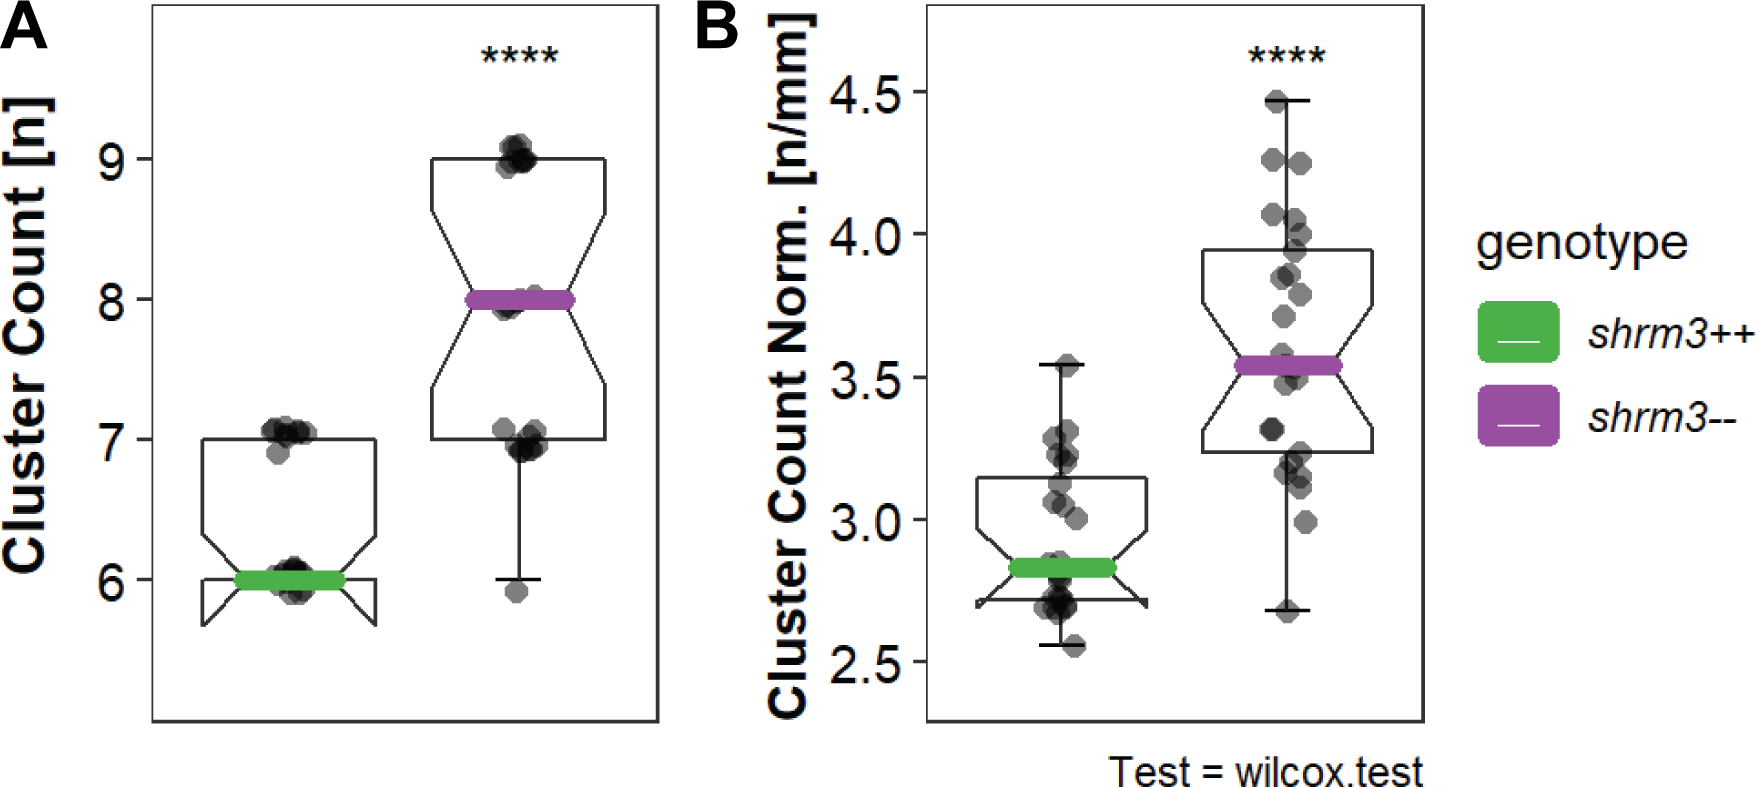
\includegraphics[width=0.6\textwidth]{figures/results/01_morphometrics/ll_counts} 

}

\caption[Cluster Counts]{Cluster counts \textbf{A} cluster count \textbf{B} normalized to length (LL length {[}µm{]} / cluster count {[}n{]})}\label{fig:llcounts}
\end{figure}
Even though CC position in individual \emph{shroom3}\(--\) embryos seems more random, the position of the first deposited CC is mostly conserved (\ref{fig:llpos}A), \(p\) for difference in position = 0.2). Similarly, the position of the pLLP also isn't significantly changed. While for the remaining CCs an average lag of -50.4 \(\mu\)m as compared to \emph{shroom3}++ CC positions is observed, it also seems to increase with later CC positions. For \emph{shroom3}++ embryos CC position is mostly conserved through development, however it remains elusive if this is true for \emph{shroom3}\(--\) embryos too.
Figure \ref{fig:llpos}A', shows the kernel density distribution for the CC position without grouping individual positions. At a binwidth of 50 \(\mu\)m, the distribution curves show a high and narrow density at around 350 \(\mu\)m, which is the average location of CC1 (\ref{fig:llpos} 2A). For the remaining CCs the kernel distribution does, neither for \emph{shroom3}++ nor for \emph{shroom3}\(--\) embryos, reveal a precise location. In contrast, if based on CC sequential identity the mean position and standard deviation is calculated, a more explicit pattern emerges which clearly shows the increased count and average frequency (\ref{fig:llpos} 2A).


\begin{figure}

{\centering 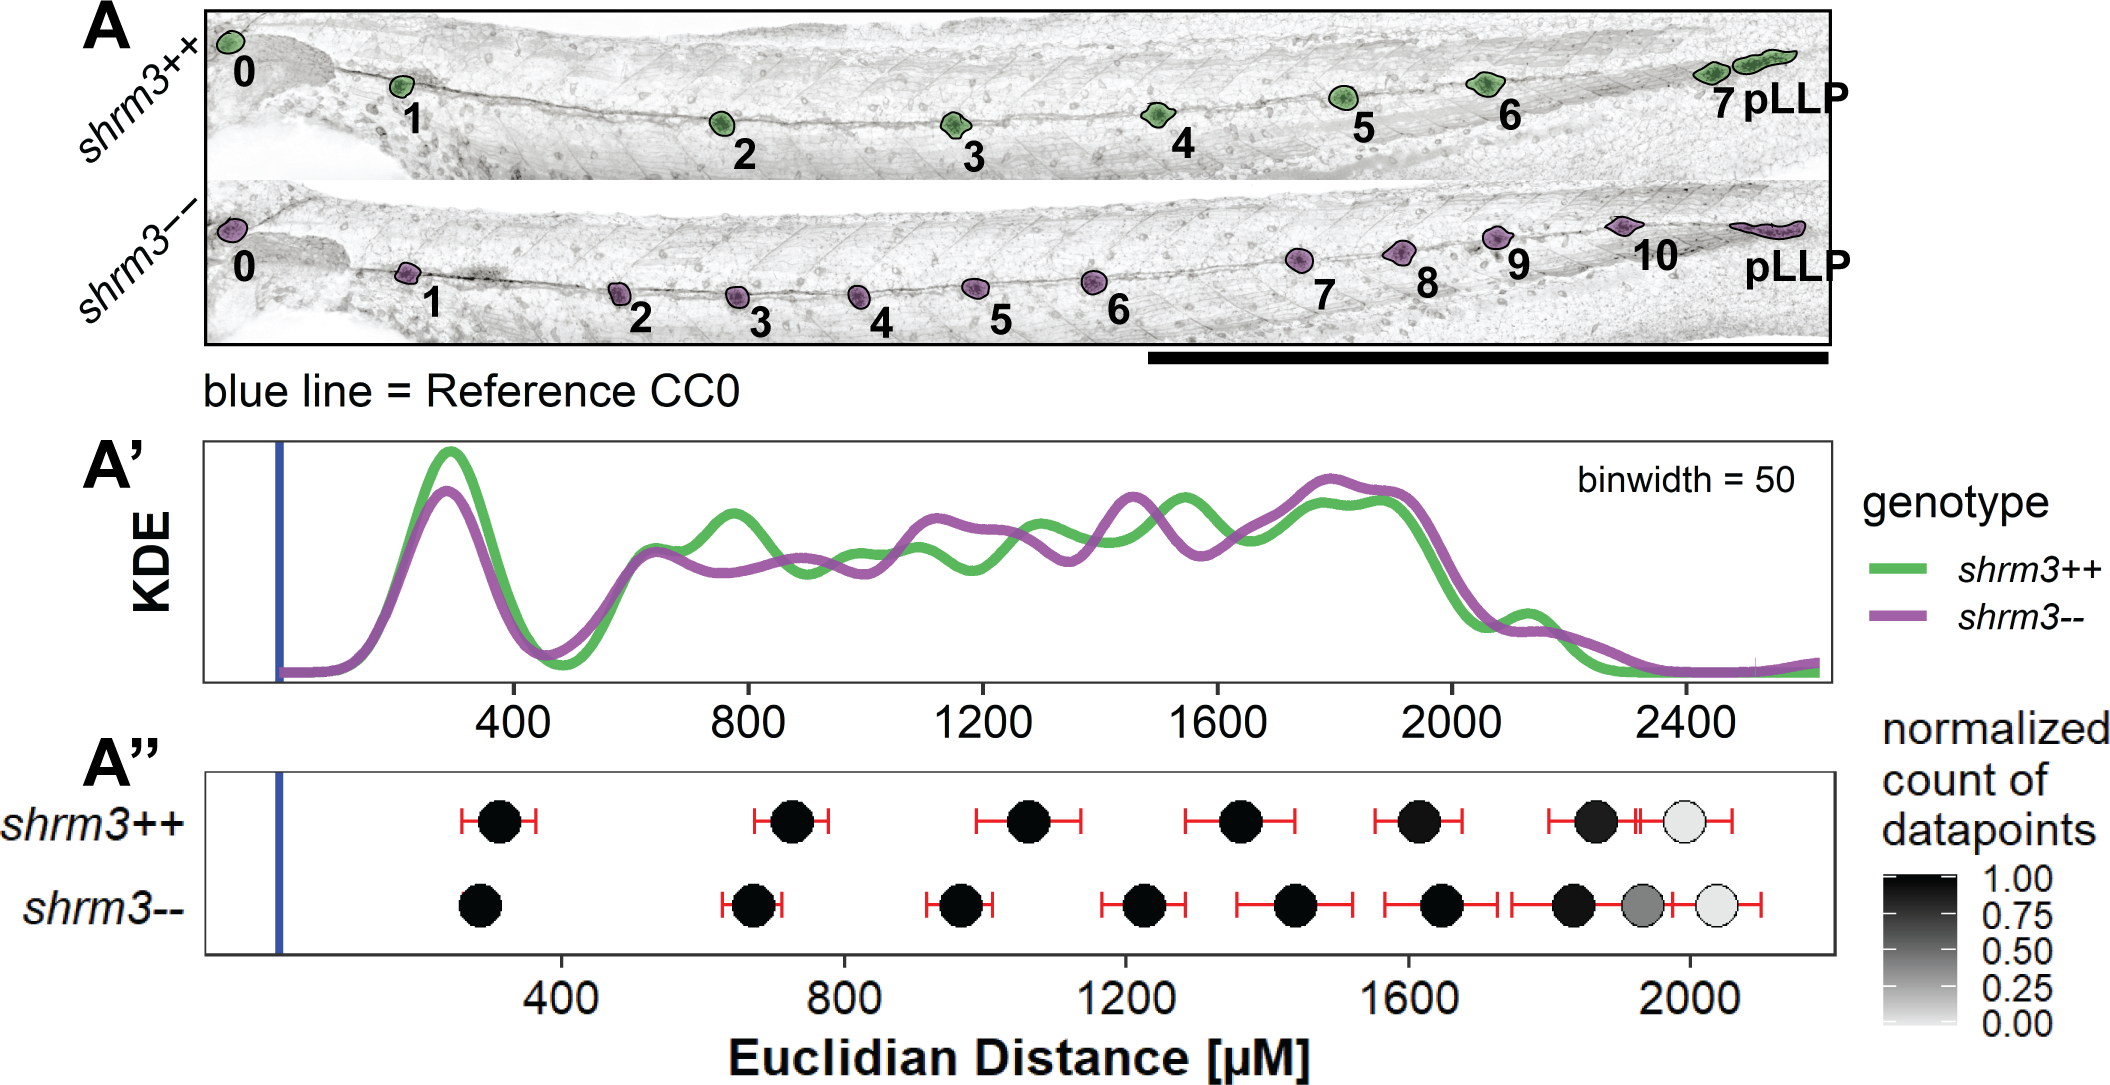
\includegraphics[width=0.85\textwidth]{figures/results/01_morphometrics/ll_positions} 

}

\caption[Cell Cluster Positions]{Cell Cluster positions \textbf{A} Exemplary \emph{shroom3}++ and \(--\) embryos with CCs hightlighted. CC0 marks the reference location to compare individual embryos. Scale bar = 1 mm \textbf{A'} Kernel Density Estimate without (KDE) grouping (n++=162, n--=206) \textbf{A''} Dots = mean positions, bars = standard deviation (nmax for both ++ and -\/- =26).}\label{fig:llpos}
\end{figure}
\hypertarget{res-llmorph}{%
\subsection{Cell Count and Area of CCs}\label{res-llmorph}}

To get an idea about whether facilitated proliferation contributes to the phenotype we observe in \emph{shroom3}\(--\) embryos, the cell count per CC was determined by counting DAPI stained cells within CC segments derived from the \emph{cldnb:lyn-gfp} membrane signal (section \ref{mat-GrTrDat}). Both cells per CC and area per CC are shrunk by about 6\% in \emph{shroom3}\(--\) embryos, while the density of cells per area remains unchanged (\ref{fig:llclus}A). Interestingly, when comparing net cell counts per embryo an increase of 9\% is observed (\ref{fig:llclus}B). Both the sum of CC cells and total LL cells (CC+pLLP) are significantly increased in \emph{shroom3}\(--\) embryos, while the count of only pLLP cells remains unchanged.


\begin{figure}

{\centering 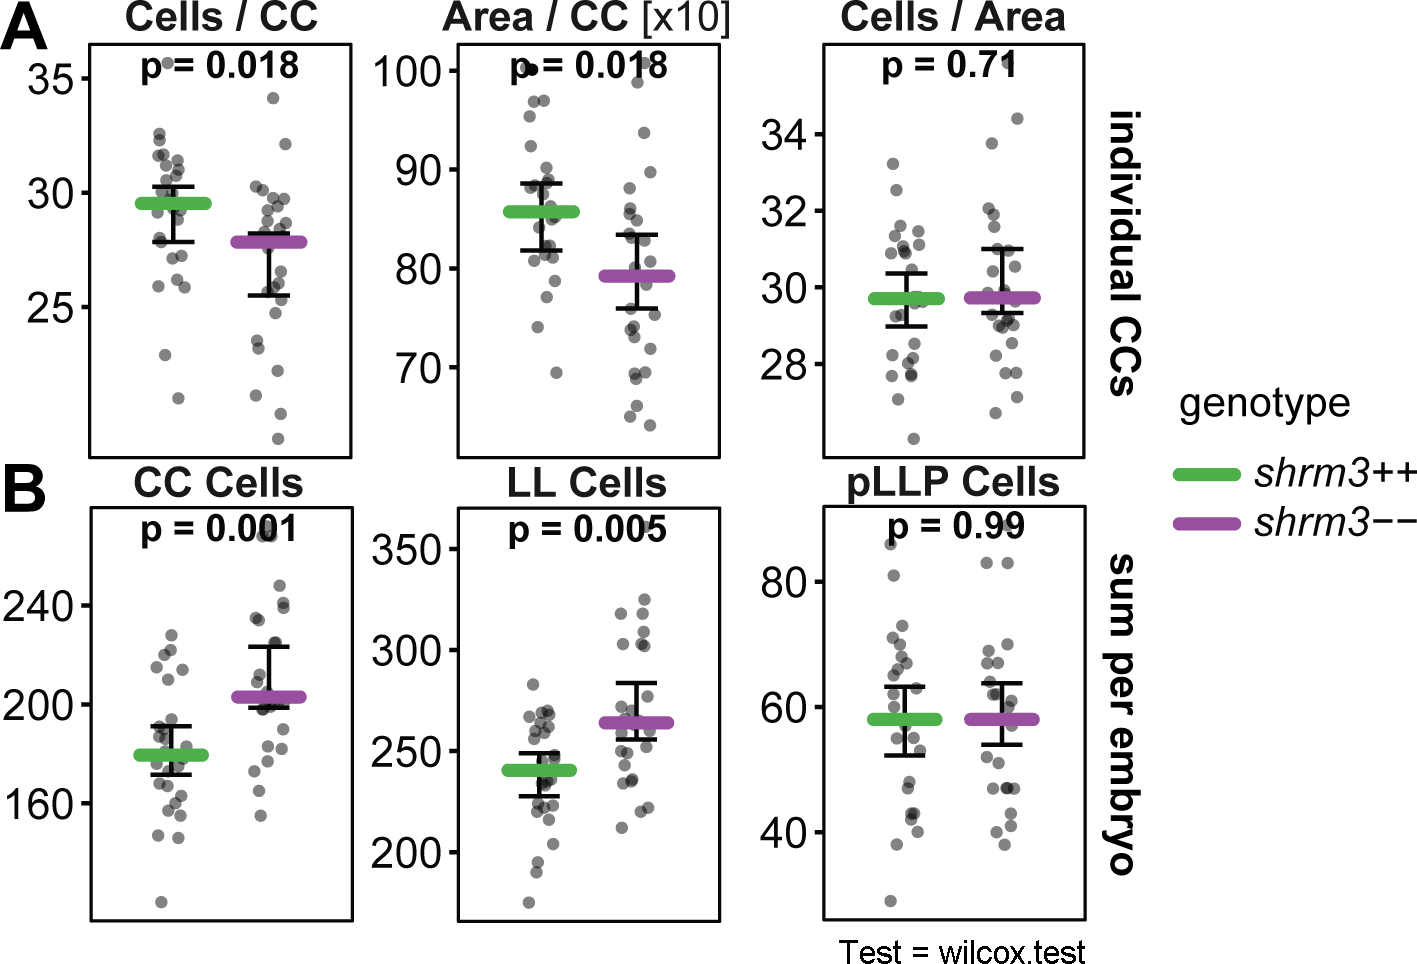
\includegraphics[width=0.7\textwidth]{figures/results/01_morphometrics/ll_clusters} 

}

\caption[LL Morphometrics]{LL Morphometrics \textbf{A} individual CC statistics \textbf{B} Sums per embryo. (Bars = median, errorbars = 95\% CI)}\label{fig:llclus}
\end{figure}
\hypertarget{proliferation}{%
\section{Proliferation}\label{proliferation}}

LL morphometric analysis revealed that deposited CCs in \emph{shroom3}\(--\) embryos were on average slightly smaller and had fewer cells incorporated. However, due to the additional two cell clusters deposited, the net count is \textasciitilde{}9\(\%\) increased at the end of migration.
To test whether this is due to higher proliferative activity a dataset of time-lapse movies (12 h / \(\Delta\)T = 6 min.) was generated to count the number of mitoses in a \emph{cxcr4b(BAC):H2BRFP} transgenic background similar to previous proliferation studies in the pLLP (\emph{23}, \emph{57}).

\hypertarget{dataset-1}{%
\subsection{Dataset}\label{dataset-1}}

The dataset consists of 12 \emph{shrm3}++ and 18 \emph{shrm3}\(--\) embryos with about 75 timepoints for the pLLP and 150 for cell clusters. For counting, tracks were created for each proliferative cell on MaxIPs (section \ref{prolif}). Figure \ref{fig:prolpllp}A shows a \emph{shroom3}++ and a \emph{shroom3}\(--\) LL after 12 h of imaging where each mitotic track is individually colored and overlaid to the image data.

To index the proliferative activity (minutes per mitosis) per embryo, the product of total number of timepoints and \(\Delta\)T in minutes was divided by the total number of mitotic events. From this we get to know the average time {[}min.{]} during which one mitosis occurs.\newline

\makebox[\linewidth]{$Proliferation\ Index = \frac{Mitotses[\mathbb{n}]}{Timepoints[ \mathbb{n}] * \Delta T [ \mathbb{min.}]}$}

\hypertarget{res-prolpllp}{%
\subsection{Lateral Line Mitoses}\label{res-prolpllp}}

Tracking mitoses in the pLLP does not reveal any difference in proliferation from start (\textasciitilde{}28 hpf) till about mid of migration 12 hours later (\ref{fig:prolpllp}B). For confirmation, this finding was also validated via two more traditional methods. During mitosis genetic material is replicated in S-phase\footnote{`S` like ‚Synthesis`}, while in meta-phase chromosomes are found to be heavily phosphorylated (\emph{58}). With an EdU\footnote{5-Ethynyl-2'-deoxyuridine} assay (\emph{59}) cells in S-phase can be detected (\ref{fig:prolpllp}B'). Using a specific phospho-histone (p-Hist.) antibody cells in meta-phase can be detected. When comparing the relative numbers of EdU resp. p-Hist cells over total pLLP cells, again, no difference in proliferation can be detected. Still, at end of migration the LL system in \emph{shroom3}\(--\) embryos does incorporate 9\(\%\) more cells.


\begin{figure}

{\centering 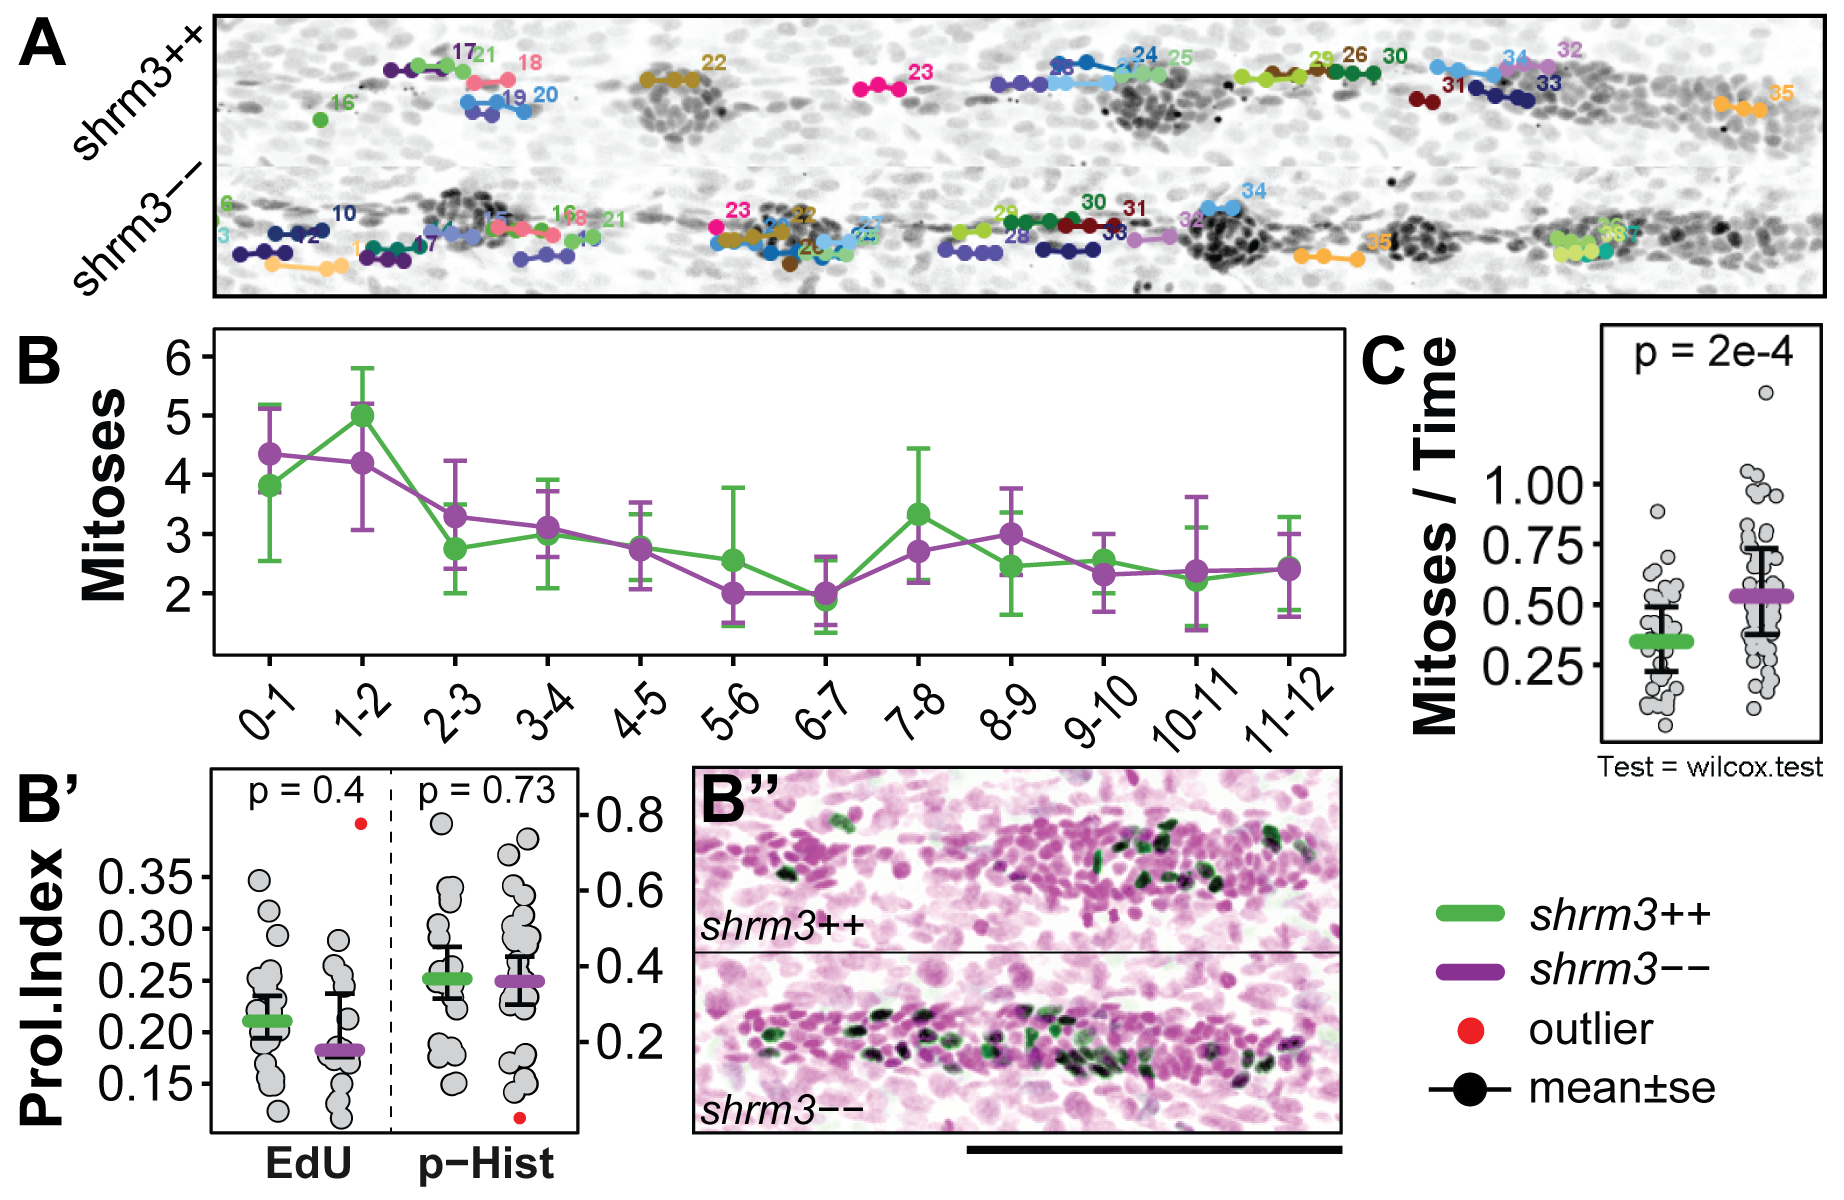
\includegraphics[width=0.85\textwidth]{figures/results/02_proliferation/prol-01} 

}

\caption[pLLP proliferation]{pLLP proliferation \textbf{A} Tracks of Mitosis. (Image data) Last timepoint of Z-projected time-lapse movie. (Labels) each dots marks a mitotic events. Each color represents one mitosis. Each connection between two dots represents 6 min. \textbf{B-B''} Mitoses in the pLLP. (B) Count of Mitoses through time (mean\(\pm\)sd) (B') Proliferation Index at 36 hpf for EdU and phospho Histone labeled pLLPs (B'`) Examples of EdU staining (scale bar = 100 \(\mu\)m) \textbf{C} Mitoses in Cell Clusters. B' and C, the colored bar indicated the median, bars indicate the 95\% CI.}\label{fig:prolpllp}
\end{figure}
Due to their high regenerative ability, zebrafish are a popular model in regenerative research (\emph{19}, \emph{22}, \emph{60}). It is well known that zebrafish NMs have a very high regenerative capacity (\emph{61}--\emph{63}). Since individual \emph{shroom3}\(--\) CCs are smaller, we wondered if there could be compensation mechanisms activated that increase proliferation to restore wildtype CC size once they are deposited. To verify this, CC mitoses were tracked on the same data as before. Other than the pLLP, which can be observed throughout the time-lapse, CCs only begin to \emph{exist} when they are deposited. To normalize for individual CC lifetimes, the number of mitoses per CC is divided by the duration of the total time-lapse minus the time span to when it first appeared. This way it becomes evident that the additional cells in \emph{shroom3}\(--\) embryos are derived from CC proliferation, rather than pLLP proliferation (\ref{fig:prolpllp}C).

\hypertarget{rosette-formation-and-cluster-deposition}{%
\section{Rosette Formation and Cluster Deposition}\label{rosette-formation-and-cluster-deposition}}

Having shown that the additional CC deposition in \emph{shroom3}\(--\) embryos is not caused by an over-proliferation in the migrating pLLP, the next step was to have a closer look at the dynamics of rosette formation, in relation to pLLP morphometrics and CC deposition. To test dependencies between different observations and developmental dynamics, variables can be correlated. To do this and to have a coherent dataset to work with, the data of three different analyses on a single set of image data were merged.
First, to get to know the exact timing of CC deposition, a manual tracking tool (\emph{53}) was used (\ref{fig:rdt}, Tracking). Second, to deduce pLLP morphometrics a self-made IJ macro (\emph{64}) was developed\footnote{anaLLzr2DT - \url{https://github.com/KleinhansDa/anaLLzr2DT}} for spatiotemporal registration of the pLLP and to yield information about its speed, area, roundness, etc. (\ref{fig:rdt}, Registration). Third, to detect rosettes and quantify their weights\footnote{as a decimal from 0-1 (1 being a wild-type rosette). For further info see section \ref{CNN}}, a CNN (\emph{65}) was used on the registered pLLP output from the anaLLzr2DT (\ref{fig:rdt}, Detection). Finally, all three datasets were merged by a unique identifier for each datapoint by a unique identifier for each embryo and timepoint.

\hypertarget{dataset-2}{%
\subsection{Dataset}\label{dataset-2}}

The image data set analyzed consists of 20 time-lapse movies (11 \emph{shroom3}\(--\), 9 \emph{shroom3}++). Each time-lapse has a duration of \textasciitilde{}20 h (\textasciitilde{}8 min. interval)\footnote{for further details about dataset acquisition see section @(refdetect-data)}, summing up to \textasciitilde{}1650 \emph{shroom3}\(--\), and \textasciitilde{}1350 \emph{shroom3}++ timepoints.


\begin{figure}

{\centering 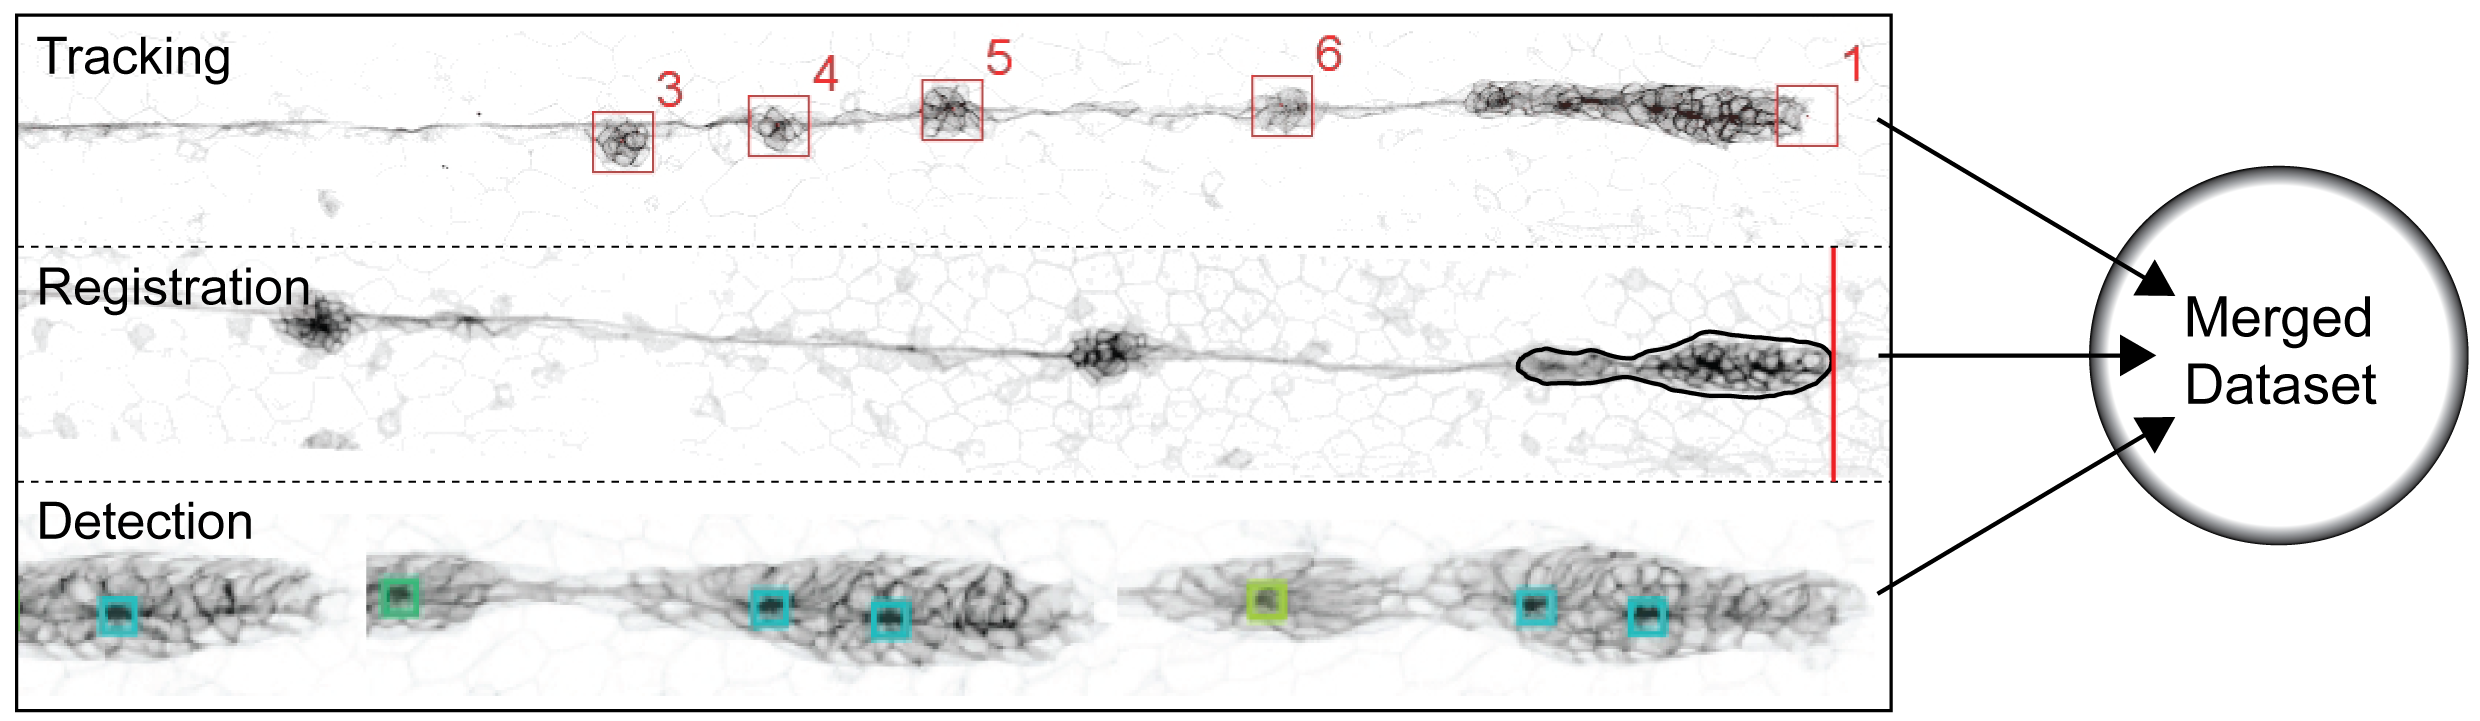
\includegraphics[width=0.7\textwidth]{figures/results/03_rosettes/RDT-01} 

}

\caption[RDT Merged Datasets]{Merged Datasets. (Tracking) pLLP is marked as no.1. The rest of the CCs is numbered sequentially as they appear. (Registration) The black outline marks the region of interest (ROI) that is the pLLP as it is detected by the anaLLzr2DT. The red line highlights the pLLPs leading edge. (Detection) Each square highlights a detected rosette by the CNN, colors represent rosette weights.}\label{fig:rdt}
\end{figure}
A full data analysis report can be found on \href{https://github.com/KleinhansDa/reports/blob/master/b7a875fc1ea228b9061041b7cec4bd3c52ab3ce3/report_RDT.html}{github}

\hypertarget{cluster-deposition}{%
\subsection{Cluster Deposition}\label{cluster-deposition}}

Figure \ref{fig:rdtdepo}A shows a montage of a \emph{shroom3}++ and a \emph{shroom3}\(--\) scenario in cluster deposition (3.5 h / \textasciitilde{}20 min. interval). For \emph{shroom3}++ the rosette structure seems tight and two depositions occur in a regular manner. In the \emph{shroom3}\(--\) on the other hand, rosette structure seems more fragile with less pronounced rosette centers and four observed depositions. Interestingly, based on the \emph{cldnb:lyn-gfp} signal the area of constriction seems to be less radially organized but more oriented towards the horizontal midline. Furthermore, the trailing rosettes are significantly smaller and do not seem to delaminate as clean from the migrating primordium. In addition, for L3 it first seems like two CCs could be deposited, until they merge again to a single CC about 1.5 h later.
On average, as it was shown before (section \ref{res-ccounts}), there's a significant increase in clusters deposited (\ref{fig:rdtdepo}B). Also, neither \emph{shroom3}++ nor \emph{shroom3}\(--\) CCs drastically change their position once they are deposited.


\begin{figure}

{\centering 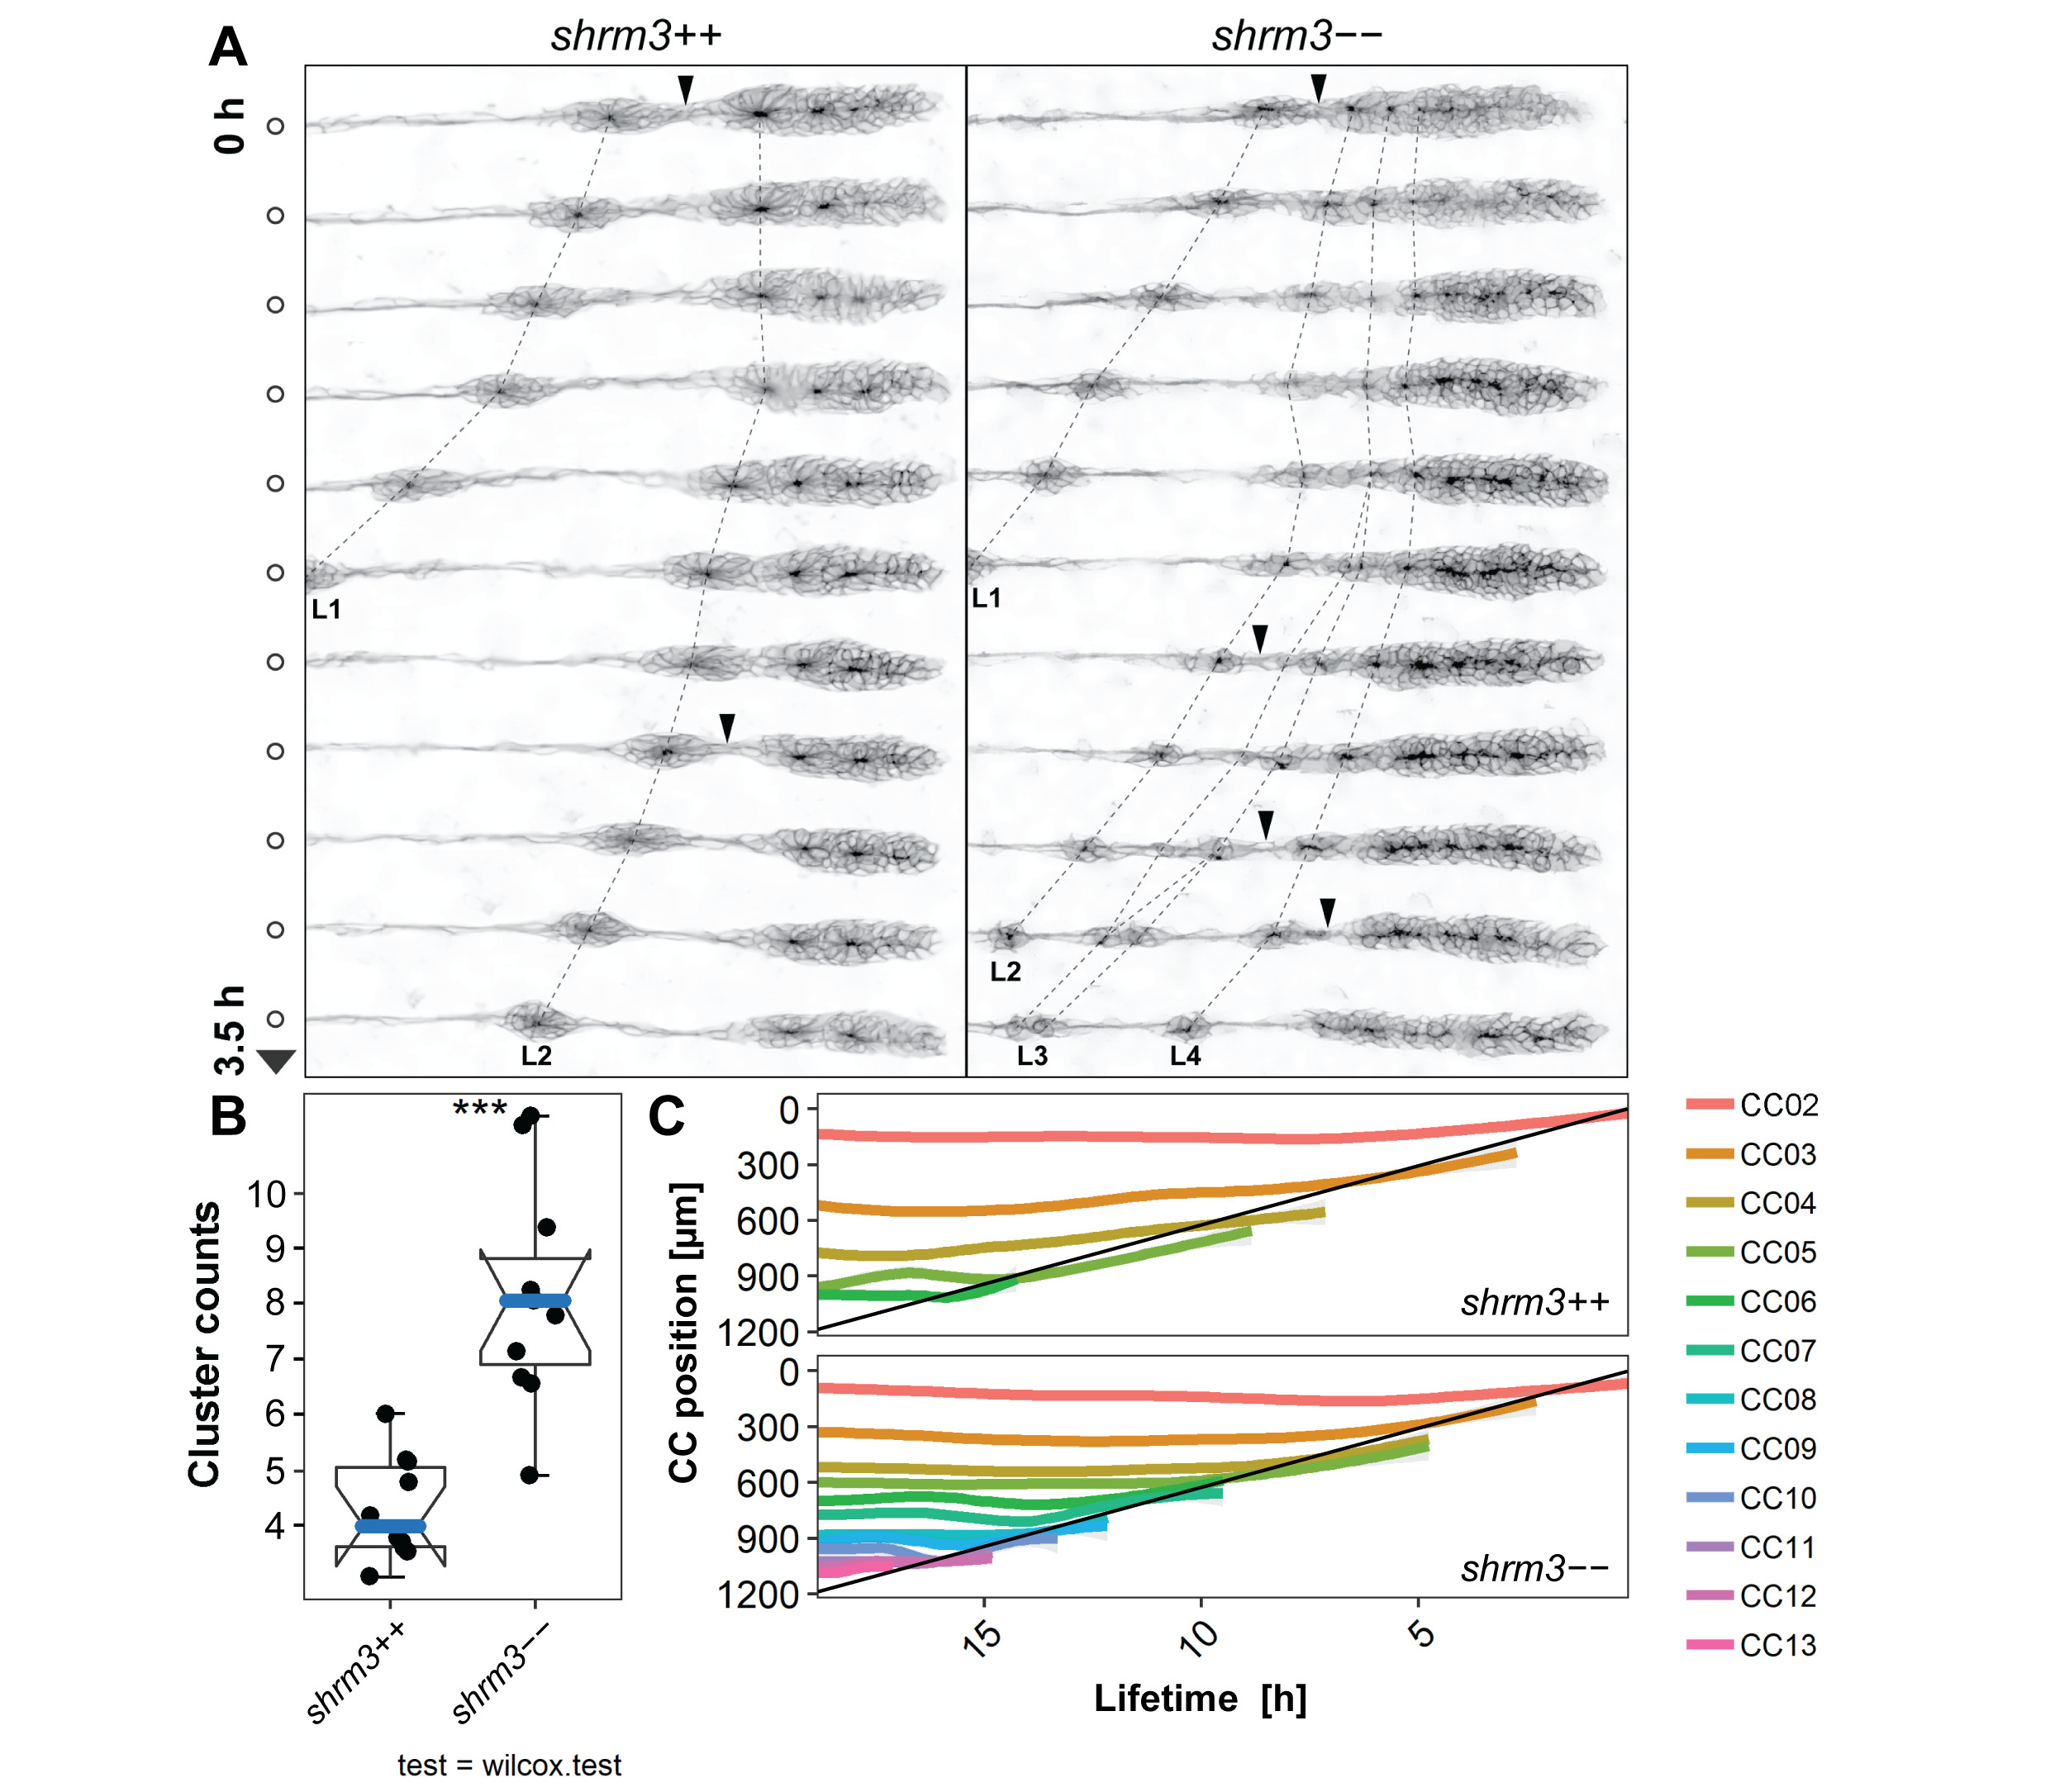
\includegraphics[width=0.95\textwidth]{figures/results/03_rosettes/tracking-01} 

}

\caption[Cluster Deposition]{Cluster Deposition \textbf{A} \emph{shroom3}++ and \emph{shroom3}\(--\) LL development in comparison. L1 - L4 are deposited CCs. Arrows indicate deposition events. Dotted lines are tracks of rosette to CC transition. \textbf{B} Statistics of deposited cluster counts \textbf{C} Change of CC position through time. Each line represents the locally weighted scatterplot smoothing (LOESS) of all CCn positions observed.}\label{fig:rdtdepo}
\end{figure}
\hypertarget{registration-1}{%
\subsection{Registration}\label{registration-1}}

As shown in figure\ref{fig:rdtreg}A-A' neither speed not acceleration drastically differ throughout the complete course of migration. Speed drops from an initial \textasciitilde{}75 \(\mu\)m/h to about \textasciitilde{}30 \(\mu\)m/h for both \emph{shroom3}++ and \emph{shroom3}\(--\) 17 h later (figure 3.3 A). Similarly, while there is a positive acceleration of almost \textasciitilde{}2 \(\mu\)m/h peaking after \textasciitilde{}2-3 hours, the remaining two peaks progressively get smaller (\ref{fig:rdtreg}A').
While for the area no difference can be detected (\ref{fig:rdtreg}B), interestingly the roundness is on average significantly reduced in \emph{shroom3}\(--\) pLLPs (\ref{fig:rdtreg}C). This is also evident from the montage in \ref{fig:rdtdepo}A.


\begin{figure}

{\centering 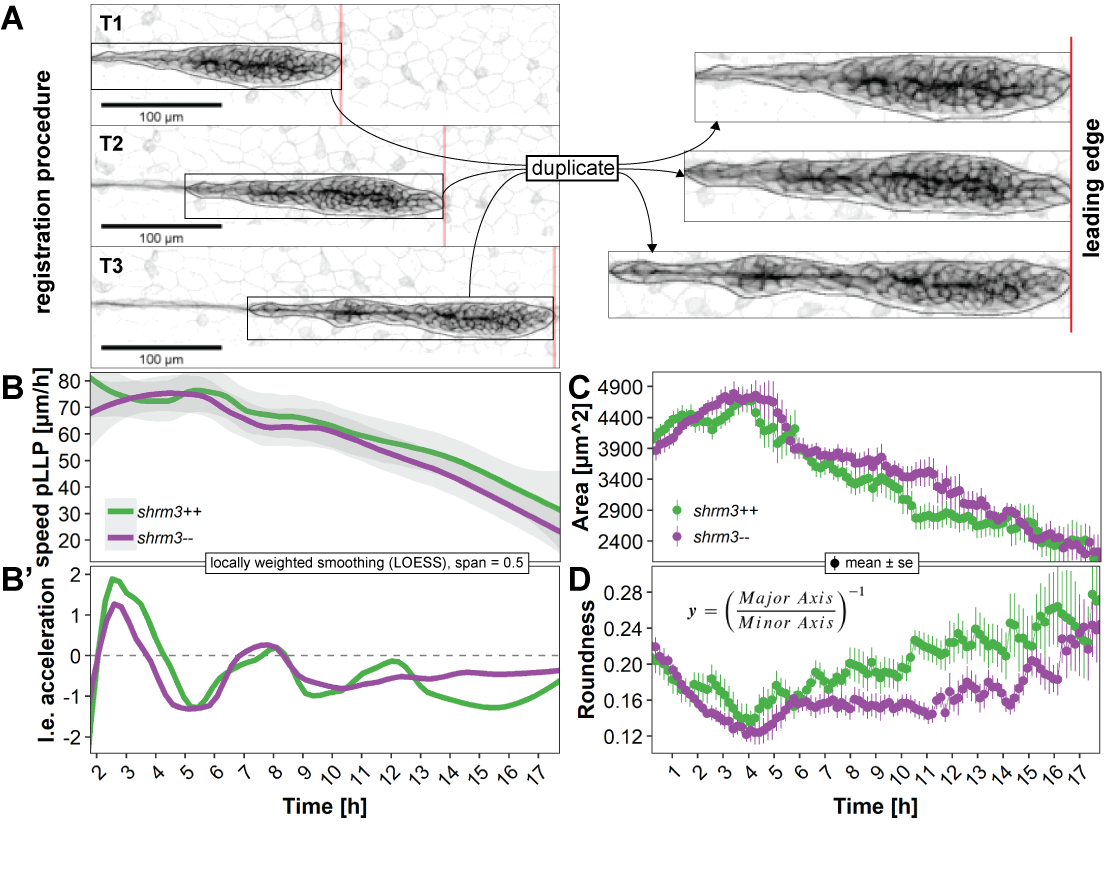
\includegraphics[width=0.95\textwidth]{figures/results/03_rosettes/registration} 

}

\caption[pLLP time-resolved morphometrics]{pLLP time-resolved morphometrics \textbf{A-A'} Leading edge (l.e.) speed and acceleration in \(\mu\)m/h, displayed as LOESS curves with at a span of 0.5 \textbf{B} Area in square \(\mu\)m and \textbf{C} Roundness displayed as mean±se (standard error).}\label{fig:rdtreg}
\end{figure}
\hypertarget{res-rdtdet}{%
\subsection{Rosette Detection}\label{res-rdtdet}}

The kymographs\footnote{a kymograph is a tool to record position over time. Here, its position of fluorescence signal intensities.} in figure \ref{fig:rdtdet}A-A' were generated on pLLPs that were registered in space and time. After registration, a line was drawn along the horizontal midline (\ref{fig:rdtreg}A). Finally, recorded kymographs were turned to false color\footnote{blue = low intensity, red = high intensity} for better visual display. In \emph{shroom3}++ the higher intensities are highly concentrated to two to three distinct regions within the migrating pLLP, while in the \emph{shroom3}\(--\) pLLP the higher intensities are more fragmented and overall reduced. To analyze this statistically all pLLPs were quantified in terms of rosette count and average rosette weight or `rosettiness' (see section \ref{CNN}).
The numbers reveal two very interesting things. First, the medians show that rosette count (\ref{fig:rdtreg}B') is only reduced for the first six hours, while rosettiness is reduced almost throughout the entire 20 hours. Second, while for rosette counts two to six indeed half or more of the pLLPs are \emph{shroom3}++, for counts below two and above six there are more \emph{shroom3}\(--\) pLLPs (\ref{fig:rdtreg}B). Furthermore figure @(fig:rdtreg)C shows that at a rosettiness of \textasciitilde{}0.7 there are about as many \emph{shroom3}++ as there are \emph{shroom3}\(--\) pLLPs, marking this point as a threshold were pLLPs above are more like likely to be \emph{shroom3}++ and below more likely to be \emph{shroom3}\(--\). At \textasciitilde{}0.1 rosettiness there are almost only \emph{shroom3}\(--\) pLLPs, while at \textasciitilde{}0.9 rosettiness there are almost only \emph{shroom3}++ pLLPs.
In addition, the data distributions attached to the sides (\ref{fig:rdtreg}B'' and C'') reveal that for the rosettiness the KDE did not actually shifted to a lower number, but rather flattened and variance is increased.


\begin{figure}

{\centering 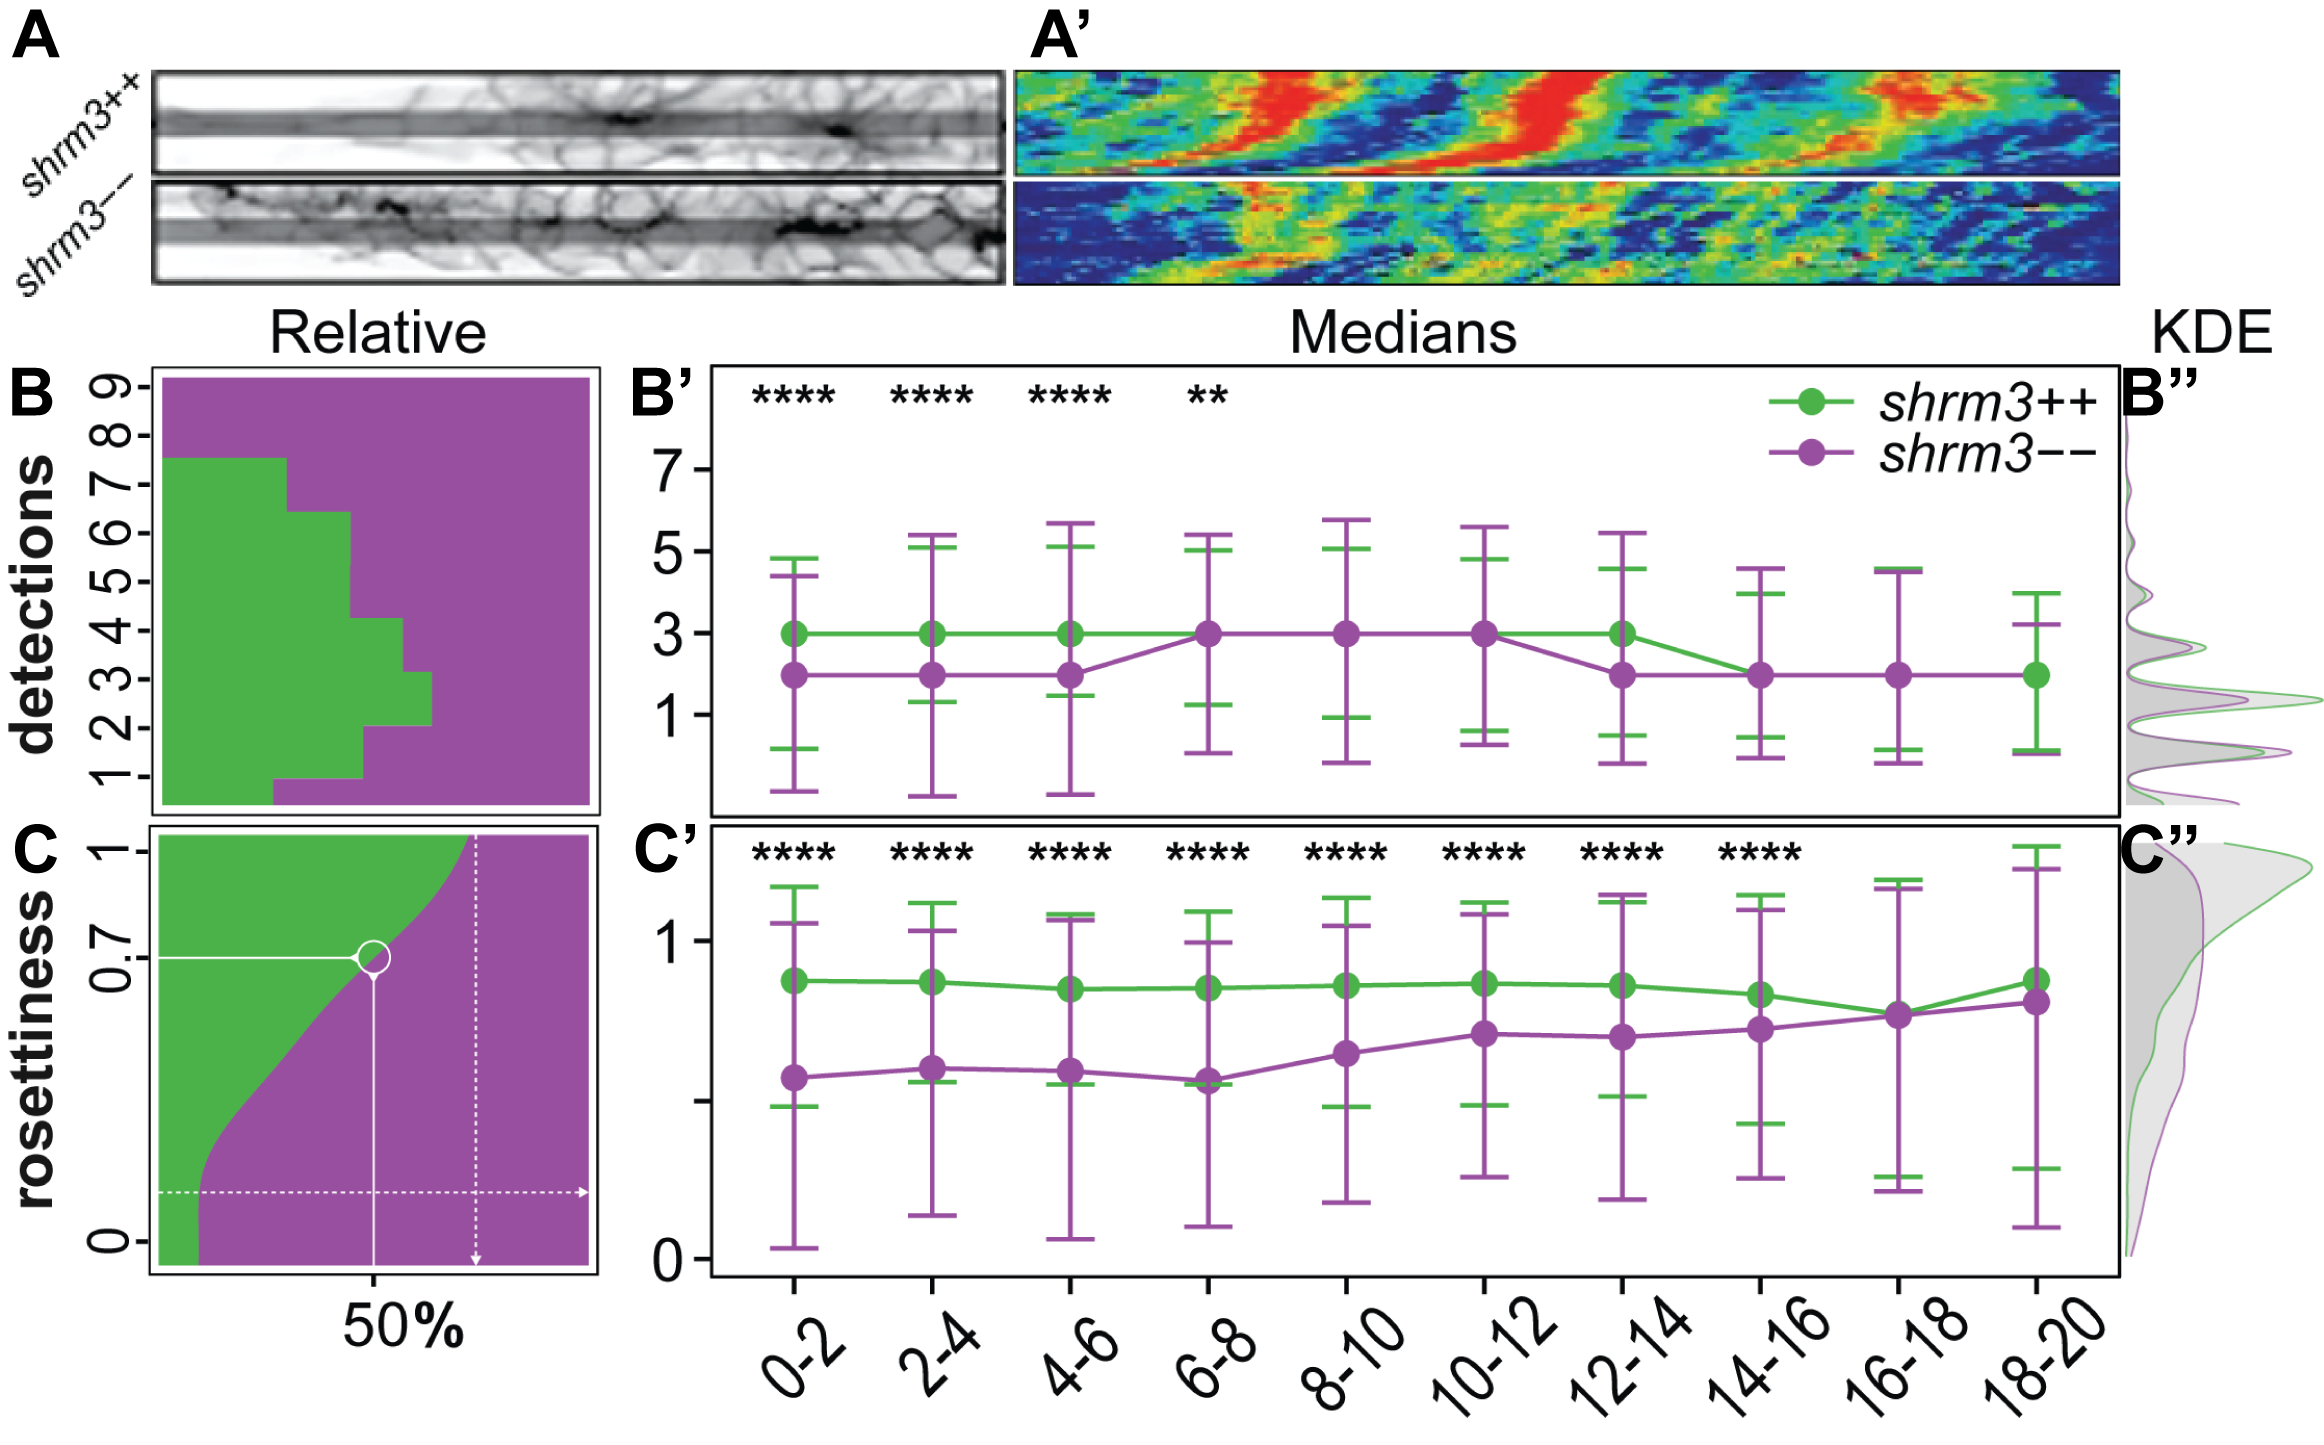
\includegraphics[width=0.95\textwidth]{figures/results/03_rosettes/detection} 

}

\caption[Rosette counts and weights]{Rosette counts and weights. \textbf{A-A'} pLLP kymographs. Length = 100 \(\mu\)m. (A) shows the signal and line drawn. (A') shows the signal through time \textbf{B-B'' and C-C''} Different graphic representation of rosette count data. (B) Filled histogram (B') Median\(\pm\)standard deviation (B'') KDE.}\label{fig:rdtdet}
\end{figure}
\hypertarget{correlations}{%
\subsection{Correlations}\label{correlations}}

The intent behind generating this combined dataset was to be able to efficiently detect interdependencies between different variables in time and space. The single dots in the scatterplots below represent the variables scatter in \(x\) and \(y\), the red line shows a linear model through the point cloud, the red digits are the correlation coefficient. Black spots with grey circles indicate the centers for clusters calculated on these two sets of data. Clustering was performed hierarchical.
For my questioning the most interesting variable to find dependencies with is rosettiness. In figure@ref(fig.rdtcorr)A and B, the \(x\) axis is occupied with the median rosettiness of all timepoints. As mentioned in section \ref{intro-phen} when we had a first closer look at the pLLP phenotype we found that a fraction of the clearly as \emph{shroom3}\(--\) identified ones still were reminiscent of the \emph{shroom3}++ phenotype. The hypothesis to test for figure \ref{fig:rdtcorr}A was that higher speeds lead to a lower degree of rosettiness and \emph{vice versa}. The correlation coefficient and model indicate a rather low interdependence. However, both also showed (\ref{fig:rdtdet}C' and \ref{fig:rdtreg}A) a high timely dependence, an effect that is lost when reducing the time dimension to the median. Interestingly, however, the line that goes through the centers determined by clustering shows is much steeper and potentially a much higher interdependence.
The hypothesis to test for figure \ref{fig:rdtcorr}B was if lower rosettiness leads to a higher number of CCs deposited and \emph{vice versa}. Since here the end of migration cluster count is one-dimensional, there is no other way than correlating to a summary statistic rosettiness. Here the correlation coefficient is rather high, the interdependence seems to be true. Additionally, the clusters determined are nicely separated from each other and the \emph{shroom3}++ and \emph{shroom3}\(--\) pLLPs seem to form two independent groups in this space.


\begin{figure}

{\centering \includegraphics[width=0.95\textwidth]{figures/results/03_rosettes/rdt_corr_speed-ros} 

}

\caption[Developmental interdependencies]{Developmental interdependencies. Digits = pearson coefficient \textbf{A} Pearson correlation coefficient between rosettiness and speed of migration through time \textbf{B} Correlation between shrm3++ and shrm3\(--\) at end of migration.}\label{fig:rdtcorr}
\end{figure}
\hypertarget{apical-constriction-1}{%
\section{Apical Constriction}\label{apical-constriction-1}}

To gain further insight into rosette assembly and the contribution of apical constriction, it is appropriate to have a closer look at rosette conformation on a cellular scale. To do so, first a set of high spatial resolution, volumetric image data was generated (XY = 0.164 \(\mu\)m / pixel; Z = 0.4 \(\mu\)m) that allowed for
\begin{enumerate}
\def\labelenumi{\arabic{enumi}.}
\tightlist
\item
  a more rigorous inspection of morphological differences, and
\item
  automated and unbiased single cell 3D reconstruction (\ref{ACI-singlecell}) using a newly developed IJ macro\footnote{anaLLzr3D - \url{https://github.com/KleinhansDa/anaLLzr3D}}. Secondly, to investigate the contribution of various single cell morphometrics to rosette formation an app was developed\footnote{LLMapR - \url{https://dskleinhans.shinyapps.io/LLmapR/}} that allows for a convenient handling of large amounts of retrieved data.
\end{enumerate}

\begin{figure}

{\centering \includegraphics[width=0.95\textwidth]{figures/results/04_constriction/reconstriction_data} 

}

\caption[High resolution, volumetric image data]{High resolution, volumetric image data. Upper row shows the fluorescence signal at the membranes. Lower row shows the 3D reconstructed cells. Columns show the same pLLP from different angles.}\label{fig:acdata}
\end{figure}
Inhibition of Fgfr1 \emph{via} drug treatment\footnote{Drug name = SU-5402 (section \ref{mat-chem})} results in a concentration dependent loss of morphogenesis and rosette assembly in the pLLP (\emph{12}, \emph{27}, \emph{55}). As a proof of principle and to validate previous studies, data of drug treated embryos (20 \(\mu\)M) and appropriate DMSO (0.1\(\%\) DMSO / E3\footnote{`Embryo Medium 3', standard zebrafish embryo incubation medium}) controls were included.

\hypertarget{dataset-3}{%
\subsection{Dataset}\label{dataset-3}}

The dataset generated consists of three pLLP stages (\ref{fig:acstages}), four groups (DMSO, SU5402, \emph{shrm3}++ and \emph{shroom3}\(--\)), 267 pLLPs and 33.163 single cells.\newline


\begin{figure}

{\centering \includegraphics[width=0.60\textwidth]{figures/results/04_constriction/Yolk_ext} 

}

\caption[Recorded developmental stages for 3D reconstruction]{Scheme showing a part of the posterior part of a zebrafish embryo and recorded developmental stages for 3D reconstruction}\label{fig:acstages}
\end{figure}
\begin{table}[t]

\caption{\label{tab:acdatatab}Apical Constriction dataset summary}
\centering
\fontsize{11}{13}\selectfont
\begin{tabu} to \linewidth {>{\raggedright}X>{\raggedright}X>{\centering}X>{\centering}X>{\centering}X}
\toprule
\multicolumn{2}{c}{\textbf{id labels}} & \multicolumn{3}{c}{\textbf{metrics}} \\
\cmidrule(l{3pt}r{3pt}){1-2} \cmidrule(l{3pt}r{3pt}){3-5}
stage & groups & pLLPs & cells & ratio\\
\midrule
 & DMSO & 20 & 2511 & 125.5\\

 & SU5402 & 19 & 2215 & 116.6\\

 & shrm3++ & 24 & 3259 & 135.8\\

\multirow[t]{-4}{*}{\raggedright\arraybackslash 32 hpf} & shrm3-- & 34 & 4281 & 125.9\\

 & DMSO & 17 & 1881 & 110.6\\

 & SU5402 & 13 & 1286 & 98.9\\

 & shrm3++ & 24 & 3144 & 131.0\\

\multirow[t]{-4}{*}{\raggedright\arraybackslash 36 hpf} & shrm3-- & 31 & 3924 & 126.6\\

 & DMSO & 18 & 2237 & 124.3\\

 & SU5402 & 13 & 1788 & 137.5\\

 & shrm3++ & 22 & 2660 & 120.9\\

\multirow[t]{-4}{*}{\raggedright\arraybackslash 40 hpf} & shrm3-- & 32 & 3977 & 124.3\\
\bottomrule
\multicolumn{5}{l}{\textit{Note: }}\\
\multicolumn{5}{l}{ratio = cells/pLLPs}\\
\end{tabu}
\end{table}
Use the sample data in the \href{https://dskleinhans.shinyapps.io/LLmapR/}{LLMapR} web-app to explore the dataset.

\hypertarget{cell-shape-and-arrangement}{%
\subsection{Cell Shape and Arrangement}\label{cell-shape-and-arrangement}}

Figure \ref{fig:acshape}B' illustrates the three developmental stages used here. For \emph{shrm3}++ pLLPs two (\ref{fig:acshape}A, 32 hpf) to four (\ref{fig:acshape}A, 40 hpf) areas of constricting regions can be observed (XZ pane), in \emph{shroom3}\(--\) its three (\ref{fig:acshape}A, 36 hpf) to seven (\ref{fig:acshape}A, 40 hpf), confirming the results of rosette detection (\ref{res-rdtdet}). While at 32 and 36 hpf the spread of those regions is wider in \emph{shroom3}\(--\), at 40 hpf they are smaller but also increased in number. When looking at the central rosette along the width (YZ pane), it seems like there is no considerable difference between \emph{shroom3}++ and \emph{shroom3}\(--\) rosettes. In SU5402 treated embryos, neither in XZ nor in YZ constriction can be observed and the cells seem to be mostly retained in their mesenchymal character and columnar shape. In addition, while constriction seems isotropic in the shroom3++ rosette center, constriction in the \emph{shroom3}\(--\) rosette center cells appears anisotropic.


\begin{figure}

{\centering \includegraphics[width=0.95\textwidth]{figures/results/04_constriction/Figure_5-1} 

}

\caption[Apical Constriction in 3D]{Apical Constriction in 3D. The stages are in columns, the groups are in rows. Each panel shows a MaxIP (top left), and orthogonal views along the length (XZ, bottom left) and along the width (YZ, right). Arrow annotations in YZ panels indicate points of constriction, bar annotations in XZ indicate the spread of region of constriction.}\label{fig:acshape}
\end{figure}
\hypertarget{single-cell-metrics}{%
\subsection{Single Cell Metrics}\label{single-cell-metrics}}

To put the above mentioned in numbers and to gain a more objective view on cell geometry, apical constriction and other metrics such as height were quantified . To get a hold on AC anisotropy we measured the length of the minor and major axis of a fit oval (\ref{fig:acaci}A). If AC was anisotropic and more cells are oriented towards the horizontal midline instead of being radially oriented, this could be shown by degrees of divergence (\(\measuredangle\)) from the horizontal midline (\ref{fig:acshape}A').
For angle measurements, all angles are normalized to a 90\(^\circ\) range, where 0\(^\circ\) is along the horizontal midline. When comparing the ratio of cells in intervals of 15\(^\circ\) along a range of 90\(^\circ\) it can be shown that there are more \emph{shroom3}\(--\) than \emph{shroom3}++ cells within the 0-15\(^\circ\) interval through all three stages (\ref{fig:acstages}). Even more, it shows that there are more \emph{shroom3}++ than \emph{shroom3}\(--\) cells within the remaining intervals -- confirming the model of constriction anisotropy.
While reduction in ACI Major is stronger than the ACI Minor in shroom3\(--\) cells (\ref{fig:acaci}C-C'), both are significantly reduced throughout time -- again confirming the increase in constriction anisotropy. The ACI for SU5402 treated embryos depicts the base value for both Major and Minor. For all three timepoints, this value stays at the same level. Interestingly, the ACI measurements for all other measurements are progressively approximating this level.


\begin{figure}

{\centering \includegraphics[width=0.95\textwidth]{figures/results/04_constriction/Figure_5-2} 

}

\caption[3D metrics and pLLP maps]{3D metrics and pLLP maps. \textbf{A-A'} Measurements. (A) Oval (black outline) represents the fit ellipse. Red arrows represent major and minor axes which are representative for A-P and D-V respectively (A') Angle measurements and intervals \textbf{B} Cellular orientation as bar chart. Statistics are indicated as stars. \textbf{C-C'} Apical Constriction measurements. Colored bars represent the median. Errorbars indicate 95\% CI.}\label{fig:acaci}
\end{figure}
\hypertarget{res-hc}{%
\section{Haircell Specification}\label{res-hc}}

Due to the rather strong cellular phenotype and overall smaller CCs we were interested if hair-cell specification would still take place and therefore if the LLs function as a sensory system would still be intact. First, to check if \emph{atoh1a} was still expressed in \emph{shroom3}\(--\) cells and if there were further implications in feedback loops with Notch signaling, an \emph{In Situ Hybridization} (ISH) experiment was conducted (probes can be found at section \ref{mat-probes}). For 36 and 40 hpf the count of \emph{atoh1a} and \emph{deltaD} expressing cells (\ref{fig:hcish}) seemed to be increased. Furthermore, especially at 40 hpf, the signal seems to be a lot more fragmented and fuzzier.
Traditional ISH allows for extremely sensitive detection of RNA transcripts on a whole embryo scale via a hybridizing anti-sense probe (section \ref{ISH-met}). However, since embryos are fixed, it only allows to analyze single time points. Furthermore, since images are taken in brightfield, there is a problem of background signal and quantification of intensity.


\begin{figure}

{\centering \includegraphics[width=0.95\textwidth]{figures/results/05_atoh/hc_ish} 

}

\caption[Expression of deltaD and atoh1a in the pLLP]{Expression of \emph{deltaD} and \emph{atoh1a} in the pLLP. Recorded in greyscale at brightfield at 20X Magnification. Images show background subtracted and de-noised EDFs of original Z-stack data.}\label{fig:hcish}
\end{figure}
To get access to developmental dynamics we made use of an additional, besides \emph{cldnb:lyn-gfp}, transgenic construct where tdTomato\footnote{Short ‚Tom`} (\emph{66}) is expressed under direct control of the \emph{atoh1a} promotor. By simultaneous observation of both fluorophores in a time-lapse setup (\ref{fig:hctl}B), the strategy was to follow up the dynamics of tom expression to count quantities and to measure the strength of expression by measuring signal intensity.

\hypertarget{dataset-4}{%
\subsection{Dataset}\label{dataset-4}}

The dataset generated consists of two groups, \emph{shroom3}++ and \emph{shroom3}\(--\), where the segmented lateral line images are split into pLLP and CC (section \ref{mat-ato-set}). Each time-lapse movie has a total duration of 18-20 hours, consists of about 54 timepoints and two channels (488 \& 561 nm).\newline
\begin{table}[t]

\caption{\label{tab:hcdatatab}Haircell specification dataset summary}
\centering
\fontsize{11}{13}\selectfont
\begin{tabu} to \linewidth {>{\raggedright}X>{\raggedright}X>{\centering}X>{\centering}X>{\centering}X}
\toprule
\multicolumn{2}{c}{\textbf{id labels}} & \multicolumn{3}{c}{\textbf{metrics}} \\
\cmidrule(l{3pt}r{3pt}){1-2} \cmidrule(l{3pt}r{3pt}){3-5}
genotype & sub-structure & embryos & timepoints & per 3h\\
\midrule
shroom3++ & pLLP & 28 & 1566 & 261\\
 & CC & 28 & 2499 & -\\
shroom3\texttt{-{}-} & pLLP & 21 & 1134 & 189\\
 & CC & 21 & 3566 & -\\
\bottomrule
\end{tabu}
\end{table}
A full data analysis report can be found on \href{https://github.com/KleinhansDa/reports/blob/master/b7a875fc1ea228b9061041b7cec4bd3c52ab3ce3/clusters_tl_tom.html}{github}

\hypertarget{atoh1a-in-the-ll}{%
\subsection{Atoh1a in the LL}\label{atoh1a-in-the-ll}}

While in both \emph{shroom3}++ and \emph{shroom3}\(--\) Tom signal intensities are rising as soon as CCs are deposited (\ref{fig:hctl}A), in \emph{shroom3}\(--\) embryos intensities are on the rise in the pLLP already in the first four hours of migration. When comparing signal intensities in deposited CCs for both, \emph{shroom3}++ and \emph{shroom3}\(--\) show a similar pattern of decreasing Tom signal intensity with progressive depositions. Similarly, when looking ungrouped overall development in CC signal intensity (\ref{fig:hctl}B), no difference can be detected.
While there is no difference in relative numbers of \emph{atoh1a} expressing cells within the migrating pLLP throughout time (\ref{fig:hctl}C), when comparing mean cell counts at specific intervals the numbers reveal a significant difference from 0 -- 3 and 12 -- 15 hours (\ref{fig:hctl}C'). The extrusions to the left in the kymographs in figure \ref{fig:hctl}D are representative to the elongating pLLP during the process of CC deposition. Magenta curves represent expression of \emph{atoh1a}. For the \emph{shroom3}\(--\) pLLP, premature expression of \emph{atoh1a} can be detected. The diagonal lines in the kymographs in figure \ref{fig:hctl}D' represent the moving pLLP along the LL. Vertical curves represent deposited CCs. As for the registered pLLP, Magenta curves represent expression of \emph{atoh1a}.


\begin{figure}

{\centering \includegraphics[width=0.95\textwidth]{figures/results/05_atoh/Figure_7-white-01} 

}

\caption[Haircell specification in the LL]{Haircell specification in the LL. \textbf{A and B} maximum Tom intensities in the pLLP and CCs. All CC lifetimes were normalized to the timepoint of deposition (timepoint zero, highlighted by striped vertical line). pLLP intensities are shows to the right, CC intensities are shows on a negative scale to the left. \textbf{C} Relative numbers of \emph{atoh1a} expressing cells and \textbf{C'} mean counts of \emph{atoh1a} expressing cells. \textbf{D-D'} Kymographs along the horizontal midline showing nascent signal of Tom (in magenta) \textbf{D} two individual pLLPs that were registered in time and to the leading edge. And \textbf{D'} Tom signal during LL development.}\label{fig:hctl}
\end{figure}
\hypertarget{rescue-experiments}{%
\section{Rescue Experiments}\label{rescue-experiments}}

Rescue experiments are focused on LL CC count and pLLP rosettiness. Since Shroom3 affects development not linearly as e.g.~a simple signaling molecule, but by providing a scaffold where different dimensions can act together, we tried rescuing by manipulating those single dimensions to find out which one had the most impact.

\hypertarget{res-shrmresc}{%
\subsection{Shroom3 Ectopic Expression}\label{res-shrmresc}}

To find out if the LL phenotype can be rescued by ectopic expression of Shroom3, a transgene was used where \emph{shroom3v1} is fused to RFP and expressed under control of a heatshock protein\footnote{In this case ‚hsp70`}. While this construct was used for rescue before (\emph{29}) (see section \ref{intro-shroom}), here it was used to test for CC count and rosettiness too. Rescuing the \emph{shroom3}\(--\) phenotype with Shroom3 itself is interesting to control for LL unspecific effects that might have happened earlier in development and to find out about Shroom3s morphogenic potential.
For this experiment, embryos were imaged two times. First at around 36 hpf, and a second time at end of migration after about 24 hours of incubation at 28.5\(^\circ\). This way it is possible to test for correlations between rosettiness earlier in development and CC count at end of migration.
While CC count is restored in heat-shocked, \emph{shroom3}\(--\), transgene carrying embryos, it also seems to reduce the number of CCs deposited in \emph{shroom3}++ (\ref{fig:rescshrm}A). For the rosettiness however, we still get a significant difference (\ref{fig:rescshrm}B). Correlation between CC count and rosettiness for heat-shocked embryos without \emph{hs:shr3v1} transgene (\ref{fig:rescshrm}C, \emph{hs:shr3v1} 00) is about the same as for embryos not heat-shocked (\ref{fig:rescshrm}C, \emph{hs:shr3v1} ??), but inverse to heat-shocked embryos with transgene (\ref{fig:rescshrm}C, \emph{hs:shr3v1} +?). Importantly, correlation is lost between heat-shocked \emph{shroom3}\(--\) embryos with transgene and not heat-shocked \emph{shroom3}++ embryos (\ref{fig:rescshrm}C, right panel). Table 3 summarizes the number of datapoints.\newline


\begin{figure}

{\centering \includegraphics[width=0.95\textwidth]{figures/results/06_rescues/shrm3/rescue_temp} 

}

\caption[shroom3 ectopic expression]{\emph{shroom3} ectopic expression \textbf{A} Normalized cluster count and statistics \textbf{B} Rosettiness and statistics \textbf{C} Correlations between beginning of migration rosettiness and end of migration cluster count}\label{fig:rescshrm}
\end{figure}
\begin{table}[t]

\caption{\label{tab:rescshrmtab}Heatshock rescue dataset summary}
\centering
\fontsize{11}{13}\selectfont
\begin{tabu} to \linewidth {>{\raggedleft}X>{\centering}X>{\centering}X>{\centering}X>{\centering}X}
\toprule
\multicolumn{3}{c}{\textbf{id labels}} & \multicolumn{2}{c}{\textbf{metrics}} \\
\cmidrule(l{3pt}r{3pt}){1-3} \cmidrule(l{3pt}r{3pt}){4-5}
treatment & genotype & transgene & CCs & LLs\\
\midrule
 & ++ / +- & Yes & 232 & 153\\

 & ++ / +- & No & 320 & \\

 & -- & Yes & 175 & \\

\multirow[t]{-4}{*}{\raggedleft\arraybackslash hs} & -- & No & 202 & \\

 & ++ / +- & Unknown & 543 & 127\\

\multirow[t]{-2}{*}{\raggedleft\arraybackslash nhs} & -- & Unknown & 354 & \\
\bottomrule
\end{tabu}
\end{table}
\begin{table}[t]

\caption{\label{tab:rescshrmsignif}Heatshock statistics}
\centering
\fontsize{8}{10}\selectfont
\begin{tabu} to \linewidth {>{\raggedright\arraybackslash}p{2cm}>{\raggedright\arraybackslash}p{2cm}>{\centering}X>{\centering}X>{\centering}X>{\centering}X>{\centering}X>{\centering}X}
\toprule
\multicolumn{2}{c}{\textbf{id labels}} & \multicolumn{3}{c}{\textbf{cluster counts}} & \multicolumn{3}{c}{\textbf{rosettiness}} \\
\cmidrule(l{3pt}r{3pt}){1-2} \cmidrule(l{3pt}r{3pt}){3-5} \cmidrule(l{3pt}r{3pt}){6-8}
group1 & group2 & p & adj.p & level & p & adj.p & level\\
\midrule
 & hs; --; tg00 & 0.01870 & 0.09300 & * & 0.00001 & 0.00012 & ****\\

 & hs; +?; tg+? & 0.00470 & 0.03300 & ** & 0.36735 & 0.73000 & ns\\

 & hs; +?; tg00 & 0.51503 & 0.60000 & ns & 0.00441 & 0.04000 & **\\

 & nhs; --; tg?? & 0.00000 & 0.00002 & **** & 0.00673 & 0.04700 & **\\

\multirow[t]{-5}{*}{\raggedright\arraybackslash hs; --; tg+?} & nhs; +?; tg?? & 0.05087 & 0.15000 & ns & 0.02962 & 0.18000 & *\\

 & hs; +?; tg+? & 0.00000 & 0.00001 & **** & 0.00000 & 0.00000 & ****\\

 & hs; +?; tg00 & 0.00208 & 0.01900 & ** & 0.00584 & 0.04700 & **\\

 & nhs; --; tg?? & 0.02068 & 0.09300 & * & 0.03663 & 0.18000 & *\\

\multirow[t]{-4}{*}{\raggedright\arraybackslash hs; --; tg00} & nhs; +?; tg?? & 0.30244 & 0.60000 & ns & 0.00002 & 0.00023 & ****\\

 & hs; +?; tg00 & 0.01018 & 0.06100 & * & 0.00008 & 0.00092 & ****\\

 & nhs; --; tg?? & 0.00000 & 0.00000 & **** & 0.00014 & 0.00160 & ***\\

\multirow[t]{-3}{*}{\raggedright\arraybackslash hs; +?; tg+?} & nhs; +?; tg?? & 0.00000 & 0.00000 & **** & 0.00086 & 0.00860 & ***\\

 & nhs; --; tg?? & 0.00000 & 0.00000 & **** & 0.66817 & 0.73000 & ns\\

\multirow[t]{-2}{*}{\raggedright\arraybackslash hs; +?; tg00} & nhs; +?; tg?? & 0.00206 & 0.01900 & ** & 0.08040 & 0.24000 & ns\\

nhs; --; tg?? & nhs; +?; tg?? & 0.00002 & 0.00024 & **** & 0.05789 & 0.23000 & ns\\
\bottomrule
\end{tabu}
\end{table}
A full data analysis report can be found on \href{https://github.com/KleinhansDa/reports/blob/master/b7a875fc1ea228b9061041b7cec4bd3c52ab3ce3/clusters_hsshrm3.html}{github}

\hypertarget{morphogen-rescue}{%
\subsection{Morphogen Rescue}\label{morphogen-rescue}}

It is known that increasing concentrations of SU5402 inhibit pLLP migration and rosette formation, leading to a reduced length of the LL system and the number of CCs deposited (\emph{12}, \emph{27}).
The idea for this experiment was to rescue the \emph{shroom3} phenotype by combining it with the phenotype of impaired Fgf signaling. Since inhibition of Fgf also reduces LL length, a titration experiment was planned to find a concentration that would not affect the length of the LL but still restore \emph{shroom3}++ levels of CC count. While concentrations 0.10 and 0.20 \(\mu\)M do not show a significant reduction in LL length, they also do not exhibit any difference in cell count.\newline


\begin{figure}

{\centering \includegraphics[width=0.95\textwidth]{figures/results/06_rescues/su54/rescue_su} 

}

\caption[Titration of Fgf inhibitor]{Titration of Fgf inhibitor \textbf{A} LL lengths are reduced with increased concentrations of Fgf inhibitor \textbf{B} Groupwise comparison of the length normalized cluster count per concentration of Fgf inhibitor.}\label{fig:rescsu}
\end{figure}
\begin{table}[t]

\caption{\label{tab:rescsutab}Morphogen rescue dataset summary}
\centering
\fontsize{11}{13}\selectfont
\begin{tabu} to \linewidth {>{\centering}X>{\centering}X>{\centering}X>{\centering}X>{\centering}X>{\centering}X}
\toprule
\multicolumn{3}{c}{\textbf{shroom3++}} & \multicolumn{3}{c}{\textbf{shroom3--}} \\
\cmidrule(l{3pt}r{3pt}){1-3} \cmidrule(l{3pt}r{3pt}){4-6}
genotype & conc. ($\mu$M) & LLs & genotype & conc. ($\mu$M) & LLs\\
\midrule
 & 0.00 & 14 &  & 0.00 & 8\\


 & 0.10 & 16 &  & 0.10 & 15\\


 & 0.25 & 24 &  & 0.25 & 21\\


 & 0.40 & 22 &  & 0.40 & 23\\


 & 0.50 & 13 &  & 0.50 & 4\\


\multirow[t]{-6}{*}{\centering\arraybackslash ++} & 1.00 & 10 & \texttt{-{}-} & 1.00 & 10\\
\bottomrule
\multicolumn{6}{l}{\textit{Note: }}\\
\multicolumn{6}{l}{concentrations in 0.1\% DMSO}\\
\end{tabu}
\end{table}
A full data analysis report can be found on \href{https://github.com/KleinhansDa/reports/blob/master/b7a875fc1ea228b9061041b7cec4bd3c52ab3ce3/clusters_su.html}{github}

\hypertarget{res-rockresc}{%
\subsection{Mechanic Rescue}\label{res-rockresc}}

It is very well known that Rho kinases are necessary for mechanic force transmission in various developmental processes (\emph{9}, \emph{33}, \emph{38}, \emph{67}, \emph{68}). Since Rock is also thought to be a key player of the Shroom force mediation pathway in the pLLP, the idea for a mechanic rescue was to titrate different concentrations of a Rock inhibitor\footnote{Rockout (section \ref{mat-chem})} and an inductor\footnote{Calyculin (section \ref{mat-chem})} to see if this way the \emph{shroom3}\(--\) phenotype can be mimicked in \emph{shroom}++ embryos resp. restored in \emph{shroom3}\(--\).

\hypertarget{rock-inhibition}{%
\subsubsection{Rock inhibition}\label{rock-inhibition}}

Embryos were incubated at distinct (figure \ref{fig:rescrock} legend) concentrations from 24 hpf till end of migration (about 60 hpf). At this stage embryos incubated at higher concentrations displayed a significant reduction in overall body length (\ref{fig:rescrock}A'). Therefore, to see if there is a lateral line specific effect on LL length, LL length was normalized to body length. Rockout treatment at 10 \(\mu\)M does not lead to a significant reduction in LL length but does significantly increase the number of cell clusters deposited.\newline


\begin{figure}

{\centering \includegraphics[width=0.95\textwidth]{figures/results/06_rescues/rockout/rescue_rockout} 

}

\caption[Titration of Rock inhibitor]{Titration of Rock inhibitor \textbf{A} LL lengths are reduced with increased concentrations of Rock inhibitor \textbf{B} Groupwise comparison of the length normalized cluster count per concentration of Fgf inhibitor.}\label{fig:rescrock}
\end{figure}
\begin{table}[t]

\caption{\label{tab:rescrocktab}Rockout rescue dataset summary}
\centering
\fontsize{11}{13}\selectfont
\begin{tabu} to \linewidth {>{\raggedleft}X>{\centering}X>{\raggedright}X}
\toprule
genotype & conc. ($\mu$M) & LLs\\
\midrule
++ & 0 & 17\\
 & 10 & 13\\
 & 50 & 17\\
 & 100 & 20\\
\bottomrule
\multicolumn{3}{l}{\textit{Note: }}\\
\multicolumn{3}{l}{concentrations in 0.1\% DMSO}\\
\end{tabu}
\end{table}
A full data analysis report can be found on \href{https://github.com/KleinhansDa/reports/blob/master/b7a875fc1ea228b9061041b7cec4bd3c52ab3ce3/clusters_rkout.html}{github}

\hypertarget{rock-induction}{%
\subsubsection{Rock induction}\label{rock-induction}}

The idea for this experiment was to rescue \emph{shroom3}\(--\) embryos by enhancing the effects of Rock. Incubation at 100 nM, the maximum solubility, does not lead any significant differences.\newline


\begin{figure}

{\centering \includegraphics[width=0.85\textwidth]{figures/results/06_rescues/caliculyn/rescue_cali} 

}

\caption[Calyculin treatment]{Calyculin treatment (A) (B)}\label{fig:resccal}
\end{figure}
\begin{table}[t]

\caption{\label{tab:resccaltab}Calyculin rescue dataset summary}
\centering
\fontsize{11}{13}\selectfont
\begin{tabu} to \linewidth {>{\centering}X>{\centering}X>{\centering}X>{\centering}X>{\centering}X>{\centering}X}
\toprule
genotype & conc. (nM) & LLs & genotype & conc. (nM) & LLs\\
\midrule
++ & 0 & 8 & \texttt{-{}-} & 0 & 8\\
 & 100 & 12 &  & 100 & 12\\
\bottomrule
\multicolumn{6}{l}{\textit{Note: }}\\
\multicolumn{6}{l}{concentrations in 0.1\% DMSO}\\
\end{tabu}
\end{table}
A full data analysis report can be found on \href{https://github.com/KleinhansDa/reports/blob/master/b7a875fc1ea228b9061041b7cec4bd3c52ab3ce3/clusters_clcln.html}{github}

\hypertarget{res-tempresc}{%
\subsection{Thermodynamic Rescue}\label{res-tempresc}}

Increasing temperature usually leads to an acceleration in thermodynamics and embryonic development, while lower temperatures decelerate (\emph{69}). Decelerated development also leads to a reduction in speed of migration and therefore to a reduction in forces that act on cells, cell-cell junctions and organ structures. In this experiment the hypothesis was that it should be possible to at least partially restore the \emph{shroom3}++ number of CCs since reduced forces would stabilize rosettes and therefore rosettes would have longer time to develop properly. Since embryos develop at different speeds, it is more challenging to exactly stage match them at end of migration. To account for this the CC count was normalized to LL length.
Even though the CC count in \emph{shroom3}\(--\) embryos incubated at 25\(^\circ\)C cannot be completely restored, they are hardly more different than levels of \emph{shroom3}++ embryos incubated at 30\(^\circ\)C.\newline


\begin{figure}

{\centering \includegraphics[width=0.75\textwidth]{figures/results/06_rescues/temp/rescue_temp} 

}

\caption[Thermodynamic rescue]{Thermodynamic rescue (A) (B)}\label{fig:resctemp}
\end{figure}
\begin{table}[t]

\caption{\label{tab:resctemptab}Thermodynamic rescue dataset summary}
\centering
\fontsize{11}{13}\selectfont
\begin{tabu} to \linewidth {>{\centering}X>{\centering}X>{\centering}X>{\centering}X>{\centering}X>{\centering}X}
\toprule
\multicolumn{3}{c}{\textbf{shroom3++}} & \multicolumn{3}{c}{\textbf{shroom3--}} \\
\cmidrule(l{3pt}r{3pt}){1-3} \cmidrule(l{3pt}r{3pt}){4-6}
genotype & treatment & LLs & genotype & treatment & LLs\\
\midrule
++ & 25°C & 18 & \texttt{-{}-} & 25°C & 19\\
 & 30°C & 15 &  & 30°C & 20\\
\bottomrule
\end{tabu}
\end{table}
\begin{table}[t]

\caption{\label{tab:resctempsignif}Thermodynamic rescue statistics}
\centering
\fontsize{8}{10}\selectfont
\begin{tabu} to \linewidth {>{\raggedright}X>{\raggedright}X>{\centering}X>{\centering}X>{\centering}X}
\toprule
group1 & group2 & p & p.adj & p.signif\\
\midrule
 & T25\_hom & 0.00000 & 0.00000 & ****\\

 & T30\_wt & 0.00747 & 0.00750 & **\\

\multirow[t]{-3}{*}{\raggedright\arraybackslash T25\_wt} & T30\_hom & 0.00000 & 0.00000 & ****\\

 & T30\_wt & 0.00104 & 0.00210 & **\\

\multirow[t]{-2}{*}{\raggedright\arraybackslash T25\_hom} & T30\_hom & 0.00015 & 0.00046 & ***\\

T30\_wt & T30\_hom & 0.00000 & 0.00000 & ****\\
\bottomrule
\end{tabu}
\end{table}
A full data analysis report can be found on \href{https://github.com/KleinhansDa/reports/blob/master/b7a875fc1ea228b9061041b7cec4bd3c52ab3ce3/clusters_temp.html}{github}

\hypertarget{atoh1a-knockdown}{%
\subsection{atoh1a knockdown}\label{atoh1a-knockdown}}

Referring back to the results we got from the hair cell analysis in section \ref{res-hc}, the hypothesis to test was if premature CC deposition in \emph{shroom3}\(--\) embryos is determined by a premature rise in Atoh1a signaling. To inhibit Atoh1a, a morpholino (MO) for \emph{atoh1a} mRNA was injected at 0.4 ng/mL, a concentration that had already been shown to be sufficient to deplete Atoh1a signaling (\emph{27}). Furthermore, since many MOs have been shown to induce cell death (\emph{70}), in a second group we co-injected embryos with an MO for p53\footnote{p53 is a gene upregulated in cancer cells, which would then self-destruct}. Interestingly injection of \emph{atoh1a} MO leads to a loss of the first CC deposited usually deposited at around 400 \(\mu\)m distance (\ref{fig:rescato}A). Furthermore, while median CC counts in \emph{atoh1a} MO injected \emph{shroom3}\(--\) embryos are actually restored to \emph{shroom3}++ levels, CC counts in \emph{shroom3}++ embryos are reduced as well.\newline


\begin{figure}

{\centering \includegraphics[width=0.95\textwidth]{figures/results/06_rescues/atoh1a/rescue_atoh} 

}

\caption[atoh1a knockdown]{atoh1a knockdown (A) (B)}\label{fig:rescato}
\end{figure}
\begin{table}[t]

\caption{\label{tab:rescatotab}Atoh rescue dataset summary}
\centering
\fontsize{11}{13}\selectfont
\begin{tabu} to \linewidth {>{\centering}X>{\centering}X>{\centering}X>{\centering}X>{\centering}X>{\centering}X}
\toprule
\multicolumn{3}{c}{\textbf{shroom3++}} & \multicolumn{3}{c}{\textbf{shroom3--}} \\
\cmidrule(l{3pt}r{3pt}){1-3} \cmidrule(l{3pt}r{3pt}){4-6}
genotype & group & LLs & genotype & group & LLs\\
\midrule
++ & p53 & 24 & \texttt{-{}-} & p53 & 22\\
 & p53+atoh1a & 22 &  & p53+atoh1a & 27\\
\bottomrule
\end{tabu}
\end{table}
\begin{table}[t]

\caption{\label{tab:rescatosignif}Atoh1a MO rescue statistics}
\centering
\fontsize{8}{10}\selectfont
\begin{tabu} to \linewidth {>{\raggedright}X>{\raggedright}X>{\centering}X>{\centering}X>{\centering}X>{\raggedright}X}
\toprule
group1 & group2 & p & p.adj & p.format & p.signif\\
\midrule
 & wt\_p53-ato & 0.00000 & 0.00001 & 0.00000 & ****\\

 & hom\_p53 & 0.00000 & 0.00000 & 0.00000 & ****\\

\multirow[t]{-3}{*}{\raggedright\arraybackslash wt\_p53} & hom\_p53-ato & 0.26803 & 0.27000 & 0.26800 & ns\\

 & hom\_p53 & 0.00000 & 0.00000 & 0.00000 & ****\\

\multirow[t]{-2}{*}{\raggedright\arraybackslash wt\_p53-ato} & hom\_p53-ato & 0.00001 & 0.00002 & 0.00001 & ****\\

hom\_p53 & hom\_p53-ato & 0.00466 & 0.00930 & 0.00470 & **\\
\bottomrule
\end{tabu}
\end{table}
A full data analysis report can be found on \href{https://github.com/KleinhansDa/reports/blob/master/b7a875fc1ea228b9061041b7cec4bd3c52ab3ce3/clusters_ato-mo.html}{github}

\hypertarget{summary-conclusion}{%
\chapter{Summary \& Conclusion}\label{summary-conclusion}}

\hypertarget{adult-phenotype}{%
\section{Adult Phenotype}\label{adult-phenotype}}

\emph{Shroom3} heterozygous zebrafish show no phenotypic abnormality. When incrossed, genotyping of two to five days post fertilization (dpf) embryos results in a Mendelian distribution. However, for stock-fish that are regenerated and genotyped by finclip at about 3 months of age show only a rate of 5-10\(\%\) of \emph{shroom3}\(--\). After another 3 -- 6 months those would usually decease too. Therefore, defect Shroom3 in \emph{D.rerio} leads to increased mortality.

\hypertarget{lateral-line}{%
\section{Lateral Line}\label{lateral-line}}

Two additional CCs are deposited in shroom3\(--\) embryos (section \ref{res-ccounts}) leading to a net increase in cell count of \textasciitilde{}9\(\%\) (31 cells) (section \ref{res-llmorph}). However, proliferation is not increased in the pLLP (section \ref{res-prolpllp}) but in CCs once they are deposited (section \ref{res-prolpllp}). Therefore, the increase in CC count is unrelated to the amount of proliferation in the pLLP. The cell count and area per CC show an average reduction of 6\(\%\) respectively and no difference for the density (section \ref{res-llmorph}).
The shroom3\(--\) LL phenotype can be mimicked by inhibition of Rock but not rescued by induction of Rock (section \ref{res-rockresc}), leading to the conclusion that Rock is necessary for proper rosette assembly and CC deposition, but not sufficient. CC count can also be rescued by ectopic expression of a Shroom3-RFP fusion protein (section \ref{res-shrmresc}), leading to the conclusion that Shroom3 has a spatiotemporal function necessary and sufficient for proper LL development.
The reduction is supported scanning electron microscopy (SEM) pictures of 3 dpf (supplement, \ref{fig:suppsem}) NMs, which indicate a disruption bundled kinocilia. However, as hair cells do still develop (supplement, \ref{fig:suppllhc}), there is no reason to presume that shroom3\(--\) NMs suffered from a loss of function. End of migration analysis also shows that the average length of the LL does not differ, suggesting that speed is not affected. This is confirmed by time-lapse analysis, which neither shows a difference in speed of migration, nor in acceleration (results, \ref{fig:rdtreg}).

\hypertarget{rosettes}{%
\section{Rosettes}\label{rosettes}}

Rosette analysis showed that the median count of rosettes is hardly (2 rosettes in \emph{shroom3}\(--\) as compared to 3 in \emph{shroom3}++ embryos) and mostly affected within the first 6-8 hours of migration ((\ref{fig:rdtdet})B and B'). Also, variance is much more affected, such that the error bars extend those of \emph{shroom3}++ in both maximum and minimum. Rosettiness however, the normalized rosette weight, is much more drastically affected ((\ref{fig:rdtdet})C and C'). While the median rosettiness of \emph{shroom3}++ is at a constant level of about 0.9, \emph{shroom3}\(--\) rosettiness starts out at about 0.5 but then linearly grows until it also reaches levels of about 0.9 at 16-20 hours of migration. As for rosette detection, variance is much higher.

Rosettiness is strongly correlated to the final number of CCs deposited (\ref{fig:rdtcorr}B) which is also evidenced by rescue of correlation between rosettiness at the beginning of migration and CC count at the end of migration (\ref{fig:rescshrm}C), concluding that rosettiness is the key parameter for the future outcome of CC pattern. Still, the question is what determines rosette weight. Although speed and rosettiness are correlated only weakly, they are significantly stronger correlated in \emph{shroom3}\(--\) than they are in \emph{shroom3}++ embryos throughout time (\ref{fig:rdtcorr}A). This finding is also confirmed by an experiment where the CC count of \emph{shroom3}\(--\) can be rescued when incubated at lower temperature (section \ref{res-tempresc}). In conclusion these results lead to the conclusion that \emph{shroom3}\(--\) rosettes are destabilized with increasing thermodynamics.

\hypertarget{hair-cells}{%
\section{Hair Cells}\label{hair-cells}}

Deposition of the first CC is more independent of Shroom3 (\ref{fig:llpos}) than the remaining CCs and the mean positions indicate that deposition does not happen more randomly, but at a higher frequency. Interestingly during the first four hours, when the first CC is deposited, analysis of hair-cell specification shows that not only the promotor for \emph{atoh1a} is more active (results, figure 5.2 A and B) in \emph{shroom3}\(--\) embryos, but also that more cells are differentiating to become hair-cells (\ref{fig:hctl}C and C'). This leads to the conclusion that the morphological changes introduced by the \emph{shroom3} mutation lead to a pre-mature activation of the \emph{shroom3} promotor, subsequently leading to deposition of the CC the hair-cell is associated with.
In the pLLP, Notch signaling is important for selection and specification of hair-cells (\ref{intro-notch}). Interestingly, these findings are supported by another study where they have shown that upon over-activated Notch signaling, CC deposition happened independent of Shroom3 (\emph{71}). For our observation this could mean that (1) either expression of \emph{atoh1a} is up-regulated due to a compensation mechanism to ensure CC deposition or (2) that the cellular rearrangements lead to biased Notch signaling. A phenomenon that in fact has been well studied (\emph{4}). For the latter, the proposed model would be that in each micro-rosette the hair-cell is in contact with less cells, but the amount of Notch ligand stays the same. Therefore, lateral inhibition and feedback is stronger, leading to an increase in expression of \emph{atoh1a} and ultimately to earlier CC deposition.

\hypertarget{apical-constriction-2}{%
\section{Apical Constriction}\label{apical-constriction-2}}

The method developed to quantify AC allows measurement along two orthogonal axes, the major (the longer axis) and a minor (the shorter axis), of an ellipse fitted to a cellular cross-section at a distinct distance from the apical site. In addition, the cells orientation in degrees from the horizontal midline is obtained (\ref{fig:acaci}A-A').

In summary, AC is significantly reduced in \emph{shroom3}\(--\) embryos for the severe phenotype. In more detail the results show an increased axial an-isotropy, meaning that AC is more reduced along the major than along the minor axis. In conclusion this means that AC and probably tension is more relaxed along the anterior-posterior axis. In terms of cell shape this means that rosette cells go from a pyramidal geometry, more to a prism geometry (\ref{fig:sumcells}). This is also confirmed by angular measurement which show that for 0-15\(^\circ\) more \emph{shroom3}\(--\) pLLPs cells are aggregated while at 30-45\(^\circ\), more \emph{shroom3}++ cells are aggregated.


\begin{figure}

{\centering \includegraphics[width=0.95\textwidth]{figures/summary/cell-model} 

}

\caption[Rosette and Cell Shape Model]{Rosette and Cell Shape Model}\label{fig:sumcells}
\end{figure}
Zona occludens-1 (ZO-1) is a peripheral membrane, tight-junction associated protein. Within the apical region of pLLP rosettes Fgf filled luminal structures are developing that that are hubs for locally confined morphogen signaling. All cells of a rosette make up and are connected to a single lumen. When visualizing the lumen via an antibody for ZO-1, the lumen appears like a buckyball where each side is the connection to a single cell (\emph{12}). While in \emph{shroom3}++ rosettes those structures appear circular in the trailing rosette, in \emph{shroom3}\(--\) rosettes they appear more oval (supplement, (\ref{fig:suppzo1}), which supports the theory of an-isotropy. Furthermore, in more leading regions the signal is more fragmented, which supports the theory of micro-rosette structures.

\hypertarget{model-2}{%
\section{Model}\label{model-2}}

Based on these results - In contrast to the current model - the \emph{shroom3}\(--\) phenotype is not defined by an absence of rosettes but by a greater than or equal to amount that are smaller and have less weight. Those `micro-rosettes' will eventually be deposited, leading to somewhat smaller CCs, which is also supported by analysis of emerging hair cells in the pLLP. The results are summarized and graphically modeled in figure 2.


\begin{figure}

{\centering \includegraphics[width=0.95\textwidth]{figures/summary/CurrentModel_new-01} 

}

\caption[Shroom3 dependent rosette formation]{Shroom3 dependent rosette formation}\label{fig:summodel}
\end{figure}
\hypertarget{discussion}{%
\chapter{Discussion}\label{discussion}}

Due to the pLLP's relative simplicity (\textasciitilde{}100 cells) and excellent accessibility for advanced light-microscopes (\textasciitilde{}1 cell layer beneath the skin), it promises an in toto understanding and complete model of factors influencing its development.
To create a robust model, it is necessary to have robust methods that allow to generate large datasets of precise and meaningful measurements. The tools and methods developed for this work have proven very useful in pinning down of essential developmental aspects and answering important biological questions with quantitative certainty. Still, due to the complexity of biological systems some points remain open for discussion.

\hypertarget{proliferation-1}{%
\section{Proliferation}\label{proliferation-1}}

For proliferation no difference in the mitotic rate could be detected in the pLLP which lead to the conclusion that additional CC deposition was independent. However, previous reports have shown a bias in location and direction of mitoses in the pLLP (\emph{23}, \emph{57}). Since our model supposed that rosette cells are more oriented along the horizontal midline this could mean that even though there are not more mitoses overall, the mitotic axis is also directed more along A-P. This in turn would result in more cells along this direction, potentially decreasing tension, leading to pre-mature deposition.

\hypertarget{rosette-detection}{%
\section{Rosette Detection}\label{rosette-detection}}

Deep learning methods are currently, driven by the hype of artificial intelligence, extremely \emph{en vogue}. While their use is not always justified, especially for biomedial image analysis they have proven extremely powerful (\emph{65}, \emph{72}, \emph{73}).

With the used fluorescent membrane label epithelial rosettes are relatively simple to detect, even with traditional image processing techniques. The arguably biggest point for criticism is that one usually does not know the features the network has learned to detect. An important metric, besides the plain detection, is the softmax-score\footnote{Also: ``detection score'', the final result of all weights of the NN}. It is a metric that tells about the security of the network how safe it is in its prediction. We interpreted this score in a way that lower prediction scores are representative for `weaker' rosettes.

\hypertarget{hair-cell-specification-1}{%
\section{Hair Cell specification}\label{hair-cell-specification-1}}

Even though the dataset for hair-cell specification provided a lot of datapoints for statistical testing, the difference for cell counts show only a relatively low significance. This could be attributed to the large variance in measurements. On the other side, not only is there a significant increase in cell count in \emph{shroom3}\(--\) pLLPs but also a higher activity of the \emph{atoh1a} promotor.

When controlling these results by trying to rescue the \emph{shroom3}\(--\) with a \emph{atoh1a} knockdown, neither in \emph{shroom3}\(--\) nor in \emph{shroom3}++ embryos the first NM is deposited anymore. Both of these results would in theory argue for an Atoh1a dependent mechanism of CC deposition, however this result has not been reported before and would need further validation. Furthermore, even though an MO for p53 was co-injected, MO injection has been shown to potentially have many more unspecific effects due to the high concentrations usually injected (\emph{74}). For this reason double mutants ( \emph{shroom3}\(--\); \emph{atoh1a}\(--\)) were generated - which at this timepoints however are not analyzed yet.

\hypertarget{single-cell-reconstruction-and-ac-measurement}{%
\section{Single cell reconstruction and AC measurement}\label{single-cell-reconstruction-and-ac-measurement}}

Earlier attempts for indexing AC include measuring the `apical index' (A.I.) of bottle cells during \emph{X.laevis} gastrulation (\emph{75}) or the ACI for cells of the pLLP (\emph{55}). For both, the metric describes the ratio of lateral height over apical width which, depending on the situation, is a very coarse and inaccurate description. In the pLLP cells of different forms, volumes and heights can be found. When measuring apical width at a fix distance from the apical site cells with different height but otherwise equal degree of AC turn out to have a very different ACI (\ref{fig:ACICells}A and A'). If however apical width is measured at a distance relative to the cells height, cells turn out to have the same ACI (\ref{fig:ACICells}A and A''). In addition, it remains questionable exactly how to define \emph{apical width} in a two-dimensional cellular cross-section. By introducing apical width measurement along both, the major and the minor axis (section \ref{ACI-pol}), the improved model for AC and method for automated and unbiased cellular segmentation therefore represents a major advancement.

AC is also correlated with cell height. To get a more detailed impression about how variables are distributed within the cells of the pLLP, single cell measurements of pLLPs that are normalized in orientation can be superimposed in a two-dimensional map of organ length and width. Next, cell coordinates in this map can be grouped into bins of hexagons and the summary statistic represented as color on a continuous scale (\ref{fig:dismap}). Doing so reveals that for stages 32 and 36 hpf, height in \emph{shroom3}\(--\) cells is not as strongly reduced as in SU5402 treated ones and that cells in the central region of the pLLP are higher than in the leading, trailing and lateral regions. In this specific case this may not lead to new insights, but it improves the visual perception and therefore may assist more concise questioning and reasoning.


\begin{figure}

{\centering \includegraphics[width=0.95\textwidth]{figures/summary/methodology_mapr} 

}

\caption[pLLP Maps]{pLLP Maps}\label{fig:dismap}
\end{figure}
In addition to visualization, large multidimensional datasets offer the possibility for advanced computational methods such as Machine- and Deep learning. For example, one could use clustering methods such as Principal Component Analysis to find out which dimensions contribute the most to separate a number of clusters from each other (\ref{fig:dispca}). Another scenario would be to manually label cells of a dataset as either leading, trailing, rosette, lateral, \ldots{} etc. to train an Machine learning model on. The model could then be used on unlabeled data to assign the previous learned labels to cells that fit the right parameters.


\begin{figure}

{\centering \includegraphics[width=0.85\textwidth]{figures/summary/pca_fig} 

}

\caption[Principal Component Analysis]{Principal Component Analysis (A) (B)}\label{fig:dispca}
\end{figure}
Yet another application example would be to use the ground truth image data generated for my studies to train a CNN that potentially would be more robust to data of different quality / resolution and easier to use as it wouldn't require as much pre-processing.

\hypertarget{future-perspectives}{%
\section{Future perspectives}\label{future-perspectives}}

\appendix

\hypertarget{supplement}{%
\chapter{Supplement}\label{supplement}}

To check whether the reduction in size and cell count of NMs in shroom3\(--\) embryos had an effect on their morphology too, scanning electron microscopy (SEM) samples for each group were imaged.


\begin{figure}

{\centering \includegraphics[width=0.50\textwidth]{figures/supp/sem} 

}

\caption[CC Kinocilia]{CC Kinocilia}\label{fig:suppsem}
\end{figure}
To check whether the reduction in size and cell count of NMs in shroom3\(--\) embryos had an effect on hair cell development, immunostainings on 4 dpf embryos with a hair cell specific marker were performed.


\begin{figure}

{\centering \includegraphics[width=0.95\textwidth]{figures/supp/ll_hc} 

}

\caption[Lateral Line Haircells]{Lateral Line Haircells}\label{fig:suppllhc}
\end{figure}

\begin{figure}

{\centering \includegraphics[width=0.75\textwidth]{figures/supp/loc} 

}

\caption[Shroom3 localization]{Shroom3 localization}\label{fig:supploc}
\end{figure}

\begin{figure}

{\centering \includegraphics[width=0.8\textwidth]{figures/supp/zo1} 

}

\caption[Luminal signaling]{Luminal signaling}\label{fig:suppzo1}
\end{figure}
An important regulator for proliferation and organ size is the mechanosensitive hippo signaling pathway where the transcription factors Yap and Taz are the most downstream targets. When dephosphorylated, Yap and Taz translocate from the cytoplasm to the nucleus to induce target gene expression.
To check for differences in hippo signaling, immunostainings for Taz were performed. On average the immunostainings suggest that Taz localization is more concentrated in the leading region and in the nuclei of peripherical PLLp cells.


\begin{figure}

{\centering \includegraphics[width=0.8\textwidth]{figures/supp/immunos} 

}

\caption[Hippo Signaling in the pLLP]{Hippo Signaling in the pLLP. PLLps with nuclei labeled in magenta and Taz in green. Vertical sections show a more basal, a medial and a more apical Z section.}\label{fig:suppyap}
\end{figure}

\begin{figure}

{\centering \includegraphics[width=0.8\textwidth]{figures/supp/Shroom3_orthology-01} 

}

\caption[Shroom Ortho- and Paralogs]{Shroom Ortho- and Paralogs}\label{fig:suppshrmort}
\end{figure}

\begin{figure}

{\centering \includegraphics[width=0.8\textwidth]{figures/supp/lim} 

}

\caption[LIM domain proteins]{LIM domain proteins}\label{fig:supplim}
\end{figure}

\begin{figure}

{\centering \includegraphics[width=0.8\textwidth]{figures/supp/partners/partners} 

}

\caption[Interaction partners fusion proteins]{Interaction partners fusion proteins \textbf{A} \emph{tagRFP-trip6} \textbf{B} \emph{tagRFP-limD1} \textbf{C} \emph{lpp-RFP}}\label{fig:supplpp}
\end{figure}

\begin{figure}

{\centering \includegraphics[width=0.8\textwidth]{figures/supp/cc_positions} 

}

\caption[Heatshock CC positions]{CC positions \textbf{A} Calyculin \textbf{B} Rockout \textbf{C} Heatshock \textbf{D} SU5402 \textbf{E} Temperature}\label{fig:supppos}
\end{figure}
The CC pattern for both \emph{shrm3}++ and \emph{shroom3}\(--\) can be modeled by a phase modulated cosine (figure 1), where the power to x represents the phase and is increased by only 0.1 in \emph{shroom3}\(--\) to go from a CC count of 5 to 7 over a span of 20 hours.


\begin{figure}

{\centering \includegraphics[width=0.8\textwidth]{figures/supp/cc_model} 

}

\caption[CC pattern model]{CC pattern model}\label{fig:supccpmodel}
\end{figure}

\begin{figure}

{\centering \includegraphics[width=0.8\textwidth]{figures/supp/gradients} 

}

\caption[Morphogenic gradients]{Morphogenic gradients}\label{fig:supgrad}
\end{figure}
\hypertarget{curriculum-vitae}{%
\chapter*{Curriculum Vitae}\label{curriculum-vitae}}
\addcontentsline{toc}{chapter}{Curriculum Vitae}

\noindent {\large \textbf{Personal information}} \hrulefill
\vspace{0.2cm}

\makebox[3cm][l]{Name:}\makebox[5cm][l]{David Kleinhans}

\makebox[3cm][l]{Adress:}\makebox[5cm][l]{Schönstraße 15}

\makebox[3cm][l]{}\makebox[5cm][l]{60327 Frankfurt am Main}

\makebox[3cm][l]{Birth details:}\makebox[5cm][l]{07.05.1988, Mannheim}

\vspace{0.3cm}

\noindent {\large \textbf{Education}} \hrulefill
\vspace{0.2cm}

\noindent \textbf{PhD studies}, Developmental Biology of Vertebrates \hfill 02.2015 -- 08.2019\newline
\emph{Goethe University, Frankfurt am Main, Germany}\newline
visiting student at \emph{Altert-Ludwigs University, Freiburg, Germany}\newline
Thesis project: \emph{Genetic and mechanic signaling during organ development}

\vspace{0.3cm}

\noindent \textbf{Master studies}, Cell Biology and Physiology \hfill 10.2012 -- 01.2015\newline
\emph{Goethe University, BMLS, Frankfurt am Main, Germany}\newline
erasmus studies at \emph{Kocaeli University, Izmit, Turkey}\newline
Thesis project: \emph{Survival window determination of Tribolium castaneum \newline exposed to different concentrations of organic compounds}

\vspace{0.3cm}

\noindent \textbf{Bachelor studies}, Molecular Biosciences \hfill 10.2008 -- 06.2012\newline
\emph{Paris Lodron University, Salzburg, Austria}\newline
visiting student at \emph{Johannes Kepler University, Linz, Austria}\newline
Thesis project: \emph{Effects of Vitamin D on the Immune System}

\vspace{0.3cm}

\noindent \textbf{Abitur} \hfill 08.1998 -- 06.2007\newline
\emph{Albertus-Magnus-Schule, Viernheim, Germany}\newline
Advanced courses: Biology, Mathematics

\vspace{0.3cm}

\noindent {\large \textbf{Additional Training}} \hrulefill
\vspace{0.2cm}

\noindent International Zebrafish and Medaka Course, KIT \hfill 05.2015

\noindent Bioimage Data Analysis, EMBL \hfill 06.2016

\noindent Analysis and Interpretation of Multivariate Data, GRADE \hfill 02.2017

\noindent Open Science for Transparent Research Practice, GRADE \hfill 05.2018

\noindent Einführung in das maschinelle lernen, GRADE \hfill 02.2019

\vspace{0.3cm}

\noindent {\large \textbf{Publications}} \hrulefill
\begin{enumerate}
\def\labelenumi{\arabic{enumi}.}
\tightlist
\item
  Nollmann, F. I., Heinrich, A. K., Brachmann, A. O., Morisseau, C., Mukherjee, K., Casanova-Torres, M., Strobl, F., Kleinhans, D., Kinski, S., Schultz, K., \emph{et al.} (2015). \href{https://onlinelibrary.wiley.com/doi/abs/10.1002/cbic.201402650}{\textbf{A Photorhabdus Natural Product Inhibits Insect Juvenile Hormone Epoxide Hydrolase.}} ChemBioChem 16, 766-771.
\end{enumerate}
\hypertarget{statutory-declaration}{%
\chapter*{\texorpdfstring{\textbf{Statutory Declaration}}{Statutory Declaration}}\label{statutory-declaration}}
\addcontentsline{toc}{chapter}{\textbf{Statutory Declaration}}

I herewith declare that I have composed the present thesis myself and without use of any other than the
cited sources and aids. Sentences or parts of sentences quoted literally are marked as such; other references
with regard to the statement and scope are indicated by full details of the publications concerned. The thesis
in the same or similar form has not been submitted to any examination body and has not been published.
This thesis was not yet, even in part, used in another examination or as a course performance.

\vskip 2cm
\centerline{\makebox[6cm][c]{\hrulefill} \makebox[0.5cm][c]{} \makebox[6cm][c]{\hrulefill}}
\centerline{\makebox[6cm][c]{Date, Place}\makebox[0.5cm][c]{} \makebox[6cm][c]{David Kleinhans}}

\backmatter

\hypertarget{references}{%
\chapter*{References}\label{references}}
\addcontentsline{toc}{chapter}{References}

\markboth{References}{References}

\noindent

\setlength{\parindent}{-0.20in}
\setlength{\leftskip}{0.20in}
\setlength{\parskip}{8pt}

\hypertarget{refs}{}
\leavevmode\hypertarget{ref-Haeckel1866}{}%
1. E. H. P. A. Haeckel, \emph{Generelle morphologie der organismen. Allgemeine grundzüge der organischen formen-wissenschaft, mechanisch begründet durch die von Charles Darwin reformirte descendenztheorie, von Ernst Haeckel.} (G. Reimer, Berlin, 1866; \url{http://www.biodiversitylibrary.org/bibliography/3953}).

\leavevmode\hypertarget{ref-Garstang1922}{}%
2. W. Garstang, The Theory of Recapitulation: A Critical Re-statement of the Biogenetic Law. \emph{J. Linn. Soc. London, Zool.} \textbf{35}, 81--101 (1922).

\leavevmode\hypertarget{ref-Davies1982}{}%
3. M. Davies, The Embodiment of the Concept of Organic Expression: Frank Lloyd Wright. \emph{Archit. Hist.} \textbf{25}, 120 (1982).

\leavevmode\hypertarget{ref-Shaya2017a}{}%
4. O. Shaya, U. Binshtok, M. Hersch, D. Rivkin, S. Weinreb, L. Amir-Zilberstein, B. Khamaisi, O. Oppenheim, R. A. Desai, R. J. Goodyear, G. P. Richardson, C. S. Chen, D. Sprinzak, Cell-Cell Contact Area Affects Notch Signaling and Notch-Dependent Patterning. \emph{Dev. Cell}. \textbf{40}, 505--511.e6 (2017).

\leavevmode\hypertarget{ref-Galli2016}{}%
5. M. Galli, D. O. Morgan, Cell Size Determines the Strength of the Spindle Assembly Checkpoint during Embryonic Development. \emph{Dev. Cell}. \textbf{36}, 344--352 (2016).

\leavevmode\hypertarget{ref-Miller2013}{}%
6. C. J. Miller, L. A. Davidson, The interplay between cell signalling and mechanics in developmental processes. \emph{Nat. Rev. Genet.} \textbf{14}, 733--744 (2013).

\leavevmode\hypertarget{ref-Thery2007}{}%
7. M. Théry, A. Jiménez-Dalmaroni, V. Racine, M. Bornens, F. Jülicher, Experimental and theoretical study of mitotic spindle orientation. \emph{Nature}. \textbf{447}, 493--496 (2007).

\leavevmode\hypertarget{ref-StJohnston2011}{}%
8. D. St Johnston, B. Sanson, Epithelial polarity and morphogenesis. \emph{Curr. Opin. Cell Biol.} \textbf{23}, 540--546 (2011).

\leavevmode\hypertarget{ref-Harding2014b}{}%
9. M. J. Harding, H. F. McGraw, A. Nechiporuk, The roles and regulation of multicellular rosette structures during morphogenesis. \emph{Development}. \textbf{141}, 2549--2558 (2014).

\leavevmode\hypertarget{ref-Niehrs2012}{}%
10. C. Niehrs, The complex world of WNT receptor signalling. \emph{Nat. Rev. Mol. Cell Biol.} \textbf{13}, 767--779 (2012).

\leavevmode\hypertarget{ref-Turner2010}{}%
11. N. Turner, R. Grose, Fibroblast growth factor signalling: From development to cancer. \emph{Nat. Rev. Cancer}. \textbf{10}, 116--129 (2010).

\leavevmode\hypertarget{ref-Durdu2014a}{}%
12. S. Durdu, M. Iskar, C. Revenu, N. Schieber, A. Kunze, P. Bork, Y. Schwab, D. Gilmour, Luminal signalling links cell communication to tissue architecture during organogenesis. \emph{Nature}. \textbf{515}, 120--124 (2014).

\leavevmode\hypertarget{ref-Bray2016}{}%
13. S. J. Bray, Notch signalling in context. \emph{Nat. Rev. Mol. Cell Biol.} \textbf{17}, 722--735 (2016).

\leavevmode\hypertarget{ref-Guisoni2017}{}%
14. N. Guisoni, R. Martinez-Corral, J. Garcia-Ojalvo, J. de Navascués, Diversity of fate outcomes in cell pairs under lateral inhibition. \emph{Dev.} \textbf{144}, 1177--1186 (2017).

\leavevmode\hypertarget{ref-Hunter2019}{}%
15. G. L. Hunter, L. He, N. Perrimon, G. Charras, E. Giniger, B. Baum, A role for actomyosin contractility in Notch signaling. \emph{BMC Biol.} \textbf{17}, 1--15 (2019).

\leavevmode\hypertarget{ref-Khait2016}{}%
16. I. Khait, Y. Orsher, O. Golan, U. Binshtok, N. Gordon-Bar, L. Amir-Zilberstein, D. Sprinzak, Quantitative Analysis of Delta-like 1 Membrane Dynamics Elucidates the Role of Contact Geometry on Notch Signaling. \emph{Cell Rep.} \textbf{14}, 225--233 (2016).

\leavevmode\hypertarget{ref-Howe2013a}{}%
17. K. Howe, M. D. Clark, C. F. Torroja, J. Torrance, C. Berthelot, M. Muffato, J. E. Collins, S. Humphray, K. McLaren, L. Matthews, S. McLaren, I. Sealy, M. Caccamo, C. Churcher, C. Scott, J. C. Barrett, R. Koch, G.-J. Rauch, S. White, W. Chow, B. Kilian, L. T. Quintais, J. a Guerra-Assunção, Y. Zhou, Y. Gu, J. Yen, J.-H. Vogel, T. Eyre, S. Redmond, R. Banerjee, J. Chi, B. Fu, E. Langley, S. F. Maguire, G. K. Laird, D. Lloyd, E. Kenyon, S. Donaldson, H. Sehra, J. Almeida-King, J. Loveland, S. Trevanion, M. Jones, M. Quail, D. Willey, A. Hunt, J. Burton, S. Sims, K. McLay, B. Plumb, J. Davis, C. Clee, K. Oliver, R. Clark, C. Riddle, D. Elliot, D. Eliott, G. Threadgold, G. Harden, D. Ware, S. Begum, B. Mortimore, B. Mortimer, G. Kerry, P. Heath, B. Phillimore, A. Tracey, N. Corby, M. Dunn, C. Johnson, J. Wood, S. Clark, S. Pelan, G. Griffiths, M. Smith, R. Glithero, P. Howden, N. Barker, C. Lloyd, C. Stevens, J. Harley, K. Holt, G. Panagiotidis, J. Lovell, H. Beasley, C. Henderson, D. Gordon, K. Auger, D. Wright, J. Collins, C. Raisen, L. Dyer, K. Leung, L. Robertson, K. Ambridge, D. Leongamornlert, S. McGuire, R. Gilderthorp, C. Griffiths, D. Manthravadi, S. Nichol, G. Barker, S. Whitehead, M. Kay, J. Brown, C. Murnane, E. Gray, M. Humphries, N. Sycamore, D. Barker, D. Saunders, J. Wallis, A. Babbage, S. Hammond, M. Mashreghi-Mohammadi, L. Barr, S. Martin, P. Wray, A. Ellington, N. Matthews, M. Ellwood, R. Woodmansey, G. Clark, J. D. Cooper, J. Cooper, A. Tromans, D. Grafham, C. Skuce, R. Pandian, R. Andrews, E. Harrison, A. Kimberley, J. Garnett, N. Fosker, R. Hall, P. Garner, D. Kelly, C. Bird, S. Palmer, I. Gehring, A. Berger, C. M. Dooley, Z. Ersan-Ürün, C. Eser, H. Geiger, M. Geisler, L. Karotki, A. Kirn, J. Konantz, M. Konantz, M. Oberländer, S. Rudolph-Geiger, M. Teucke, C. Lanz, G. Raddatz, K. Osoegawa, B. Zhu, A. Rapp, S. Widaa, C. Langford, F. Yang, S. C. Schuster, N. P. Carter, J. Harrow, Z. Ning, J. Herrero, S. M. J. Searle, A. Enright, R. Geisler, R. H. a Plasterk, C. Lee, M. Westerfield, P. J. de Jong, L. I. Zon, J. H. Postlethwait, C. Nüsslein-Volhard, T. J. P. Hubbard, H. Roest Crollius, J. Rogers, D. L. Stemple, The zebrafish reference genome sequence and its relationship to the human genome. \emph{Nature}. \textbf{496}, 498--503 (2013).

\leavevmode\hypertarget{ref-Kimmel1995a}{}%
18. C. B. Kimmel, W. W. Ballard, S. R. Kimmel, B. Ullmann, T. F. Schilling, Stages of embryonic development of the zebrafish. \emph{Dev. Dyn.} \textbf{203}, 253--310 (1995).

\leavevmode\hypertarget{ref-Chitnis2012a}{}%
19. A. B. Chitnis, D. Dalle Nogare, M. Matsuda, Building the posterior lateral line system in zebrafish. \emph{Dev. Neurobiol.} \textbf{72}, 234--255 (2012).

\leavevmode\hypertarget{ref-Ghysen2007a}{}%
20. A. Ghysen, C. Dambly-Chaudiere, The lateral line microcosmos. \emph{Genes \& Dev.} \textbf{21}, 2118--2130 (2007).

\leavevmode\hypertarget{ref-Haas2006c}{}%
21. P. Haas, D. Gilmour, Chemokine Signaling Mediates Self-Organizing Tissue Migration in the Zebrafish Lateral Line. \emph{Dev. Cell}. \textbf{10}, 673--680 (2006).

\leavevmode\hypertarget{ref-Harding2014a}{}%
22. E. D. Thomas, I. A. Cruz, D. W. Hailey, D. W. Raible, There and back again: development and regeneration of the zebrafish lateral line system. \emph{Wiley Interdiscip. Rev. Dev. Biol.} \textbf{4}, 1--16 (2015).

\leavevmode\hypertarget{ref-Laguerre2009a}{}%
23. L. Laguerre, A. Ghysen, C. Dambly-Chaudière, Mitotic patterns in the migrating lateral line cells of zebrafish embryos. \emph{Dev. Dyn.} \textbf{238}, 1042--1051 (2009).

\leavevmode\hypertarget{ref-Nechiporuk2008}{}%
24. A. Nechiporuk, D. W. Raible, FGF-dependent mechanosensory organ patterning in zebrafish. \emph{Science}. \textbf{320}, 1774--1777 (2008).

\leavevmode\hypertarget{ref-Aman2008}{}%
25. A. Aman, T. Piotrowski, Wnt/\(\beta\)-Catenin and Fgf Signaling Control Collective Cell Migration by Restricting Chemokine Receptor Expression. \emph{Dev. Cell}. \textbf{15}, 749--761 (2008).

\leavevmode\hypertarget{ref-Hava2009}{}%
26. D. Hava, U. Forster, M. Matsuda, S. Cui, B. a Link, J. Eichhorst, B. Wiesner, A. Chitnis, S. Abdelilah-Seyfried, Apical membrane maturation and cellular rosette formation during morphogenesis of the zebrafish lateral line. \emph{J. Cell Sci.} \textbf{122}, 687--695 (2009).

\leavevmode\hypertarget{ref-Lecaudey2008a}{}%
27. V. Lecaudey, G. Cakan-Akdogan, W. H. J. Norton, D. Gilmour, Dynamic Fgf signaling couples morphogenesis and migration in the zebrafish lateral line primordium. \emph{Development}. \textbf{135}, 2695--705 (2008).

\leavevmode\hypertarget{ref-Tsang}{}%
28. M. Tsang, R. Friesel, T. Kudoh, I. B. Dawid, Identification of Sef, a novel modulator of FGF signalling. \emph{Nat. Cell Biol.} \textbf{4}, 165--169 (2002).

\leavevmode\hypertarget{ref-Ernst2012a}{}%
29. S. Ernst, K. Liu, S. Agarwala, N. Moratscheck, M. E. Avci, D. D. Nogare, A. B. Chitnis, O. Ronneberger, V. Lecaudey, Shroom3 is required downstream of FGF signalling to mediate proneuromast assembly in zebrafish. \emph{Development}. \textbf{139}, 4571--4581 (2012).

\leavevmode\hypertarget{ref-Matsuda2010b}{}%
30. M. Matsuda, A. B. Chitnis, Atoh1a expression must be restricted by Notch signaling for effective morphogenesis of the posterior lateral line primordium in zebrafish. \emph{Development}. \textbf{137}, 3477--3487 (2010).

\leavevmode\hypertarget{ref-Mirkovic2012}{}%
31. I. Mirkovic, S. Pylawka, a J. Hudspeth, Rearrangements between differentiating hair cells coordinate planar polarity and the establishment of mirror symmetry in lateral-line neuromasts. \emph{Biol. Open}. \textbf{1}, 498--505 (2012).

\leavevmode\hypertarget{ref-Rouse1991}{}%
32. G. W. Rouse, J. O. Pickles, Paired development of hair cells in neuromasts of the teleost lateral line. \emph{Proc. R. Soc. B Biol. Sci.} \textbf{246}, 123--128 (1991).

\leavevmode\hypertarget{ref-Das2014a}{}%
33. D. Das, J. K. Zalewski, S. Mohan, T. F. Plageman, A. P. VanDemark, J. D. Hildebrand, The interaction between Shroom3 and Rho-kinase is required for neural tube morphogenesis in mice. \emph{Biol. Open}. \textbf{3}, 850--60 (2014).

\leavevmode\hypertarget{ref-Hildebrand2005}{}%
34. J. D. Hildebrand, Shroom regulates epithelial cell shape via the apical positioning of an actomyosin network. \emph{J. Cell Sci.} \textbf{118}, 5191--203 (2005).

\leavevmode\hypertarget{ref-Hildebrand1999a}{}%
35. J. D. Hildebrand, P. Soriano, Shroom, a PDZ Domain--Containing Actin-Binding Protein, Is Required for Neural Tube Morphogenesis in Mice. \emph{Cell}. \textbf{99}, 485--497 (1999).

\leavevmode\hypertarget{ref-Lee2007}{}%
36. C. Lee, H. M. Scherr, J. B. Wallingford, Shroom family proteins regulate gamma-tubulin distribution and microtubule architecture during epithelial cell shape change. \emph{Development}. \textbf{134}, 1431--1441 (2007).

\leavevmode\hypertarget{ref-Nishimura2008}{}%
37. T. Nishimura, M. Takeichi, Shroom3-mediated recruitment of Rho kinases to the apical cell junctions regulates epithelial and neuroepithelial planar remodeling. \emph{Development}. \textbf{135}, 1493--1502 (2008).

\leavevmode\hypertarget{ref-Plageman2011}{}%
38. T. F. Plageman, B. K. Chauhan, C. Yang, F. Jaudon, X. Shang, Y. Zheng, M. Lou, A. Debant, J. D. Hildebrand, R. a Lang, A Trio-RhoA-Shroom3 pathway is required for apical constriction and epithelial invagination. \emph{Development}. \textbf{138}, 5177--88 (2011).

\leavevmode\hypertarget{ref-Tariq2011}{}%
39. M. Tariq, J. W. Belmont, S. Lalani, T. Smolarek, S. M. Ware, SHROOM3 is a novel candidate for heterotaxy identified by whole exome sequencing. \emph{Genome Biol.} \textbf{12}, R91 (2011).

\leavevmode\hypertarget{ref-Zalewski2016}{}%
40. J. K. Zalewski, J. H. Mo, S. Heber, A. Heroux, R. G. Gardner, J. D. Hildebrand, A. P. VanDemark, Structure of the Shroom-Rho kinase complex reveals a binding interface with monomeric shroom that regulates cell morphology and stimulates kinase activity. \emph{J. Biol. Chem.} \textbf{291}, 25364--25374 (2016).

\leavevmode\hypertarget{ref-Liu}{}%
41. K. Liu, S. Ernst, V. Lecaudey, O. Ronneberger, Epithelial rosette detection in microscopic images, 1--8 (2010).

\leavevmode\hypertarget{ref-Bedell2012a}{}%
42. V. M. Bedell, Y. Wang, J. M. Campbell, T. L. Poshusta, C. G. Starker, R. G. Krug II, W. Tan, S. G. Penheiter, A. C. Ma, A. Y. H. Leung, S. C. Fahrenkrug, D. F. Carlson, D. F. Voytas, K. J. Clark, J. J. Essner, S. C. Ekker, In vivo genome editing using a high-efficiency TALEN system. \emph{Nature}. \textbf{490}, 114--118 (2012).

\leavevmode\hypertarget{ref-Keller2010c}{}%
43. P. J. Keller, E. H. K. Stelzer, Digital scanned laser light sheet fluorescence microscopy. \emph{Cold Spring Harb. Protoc.} \textbf{2010}, pdb.top78 (2010).

\leavevmode\hypertarget{ref-Graf2005}{}%
44. R. Gräf, J. Rietdorf, T. Zimmermann, in \emph{Microsc. Tech.} (Springer, 2005; \url{http://link.springer.com/10.1007/b102210}), pp. 57--75.

\leavevmode\hypertarget{ref-Haddon1998}{}%
45. C. Haddon, L. Smithers, S. Schneider-Maunoury, T. Coche, D. Henrique, J. Lewis, Multiple delta genes and lateral inhibition in zebrafish primary neurogenesis. \emph{Development}. \textbf{125}, 359--370 (1998).

\leavevmode\hypertarget{ref-Schindelin2012}{}%
46. J. Schindelin, I. Arganda-Carreras, E. Frise, V. Kaynig, M. Longair, T. Pietzsch, S. Preibisch, C. Rueden, S. Saalfeld, B. Schmid, J.-Y. Tinevez, D. J. White, V. Hartenstein, K. Eliceiri, P. Tomancak, A. Cardona, Fiji: an open-source platform for biological-image analysis. \emph{Nat. Methods}. \textbf{9}, 676--82 (2012).

\leavevmode\hypertarget{ref-Button2013}{}%
47. K. S. Button, J. P. Ioannidis, C. Mokrysz, B. A. Nosek, J. Flint, E. S. Robinson, M. R. Munafò, Power failure: Why small sample size undermines the reliability of neuroscience. \emph{Nat. Rev. Neurosci.} (2013), doi:\href{https://doi.org/10.1038/nrn3475}{10.1038/nrn3475}.

\leavevmode\hypertarget{ref-Krig2014}{}%
48. S. Krig, in \emph{Comput. Vis. Metrics} (Apress, Berkeley, CA, 2014; \href{http://link.springer.com/10.1007/978-1-4302-5930-5\%7B/_\%7D7}{http://link.springer.com/10.1007/978-1-4302-5930-5\{\textbackslash{}\_\}7}), pp. 283--311.

\leavevmode\hypertarget{ref-Legland2016}{}%
49. D. Legland, I. Arganda-Carreras, P. Andrey, MorphoLibJ: Integrated library and plugins for mathematical morphology with ImageJ. \emph{Bioinformatics} (2016), doi:\href{https://doi.org/10.1093/bioinformatics/btw413}{10.1093/bioinformatics/btw413}.

\leavevmode\hypertarget{ref-Ollion2013}{}%
50. J. Ollion, J. Cochennec, F. Loll, C. Escudé, T. Boudier, TANGO: A generic tool for high-throughput 3D image analysis for studying nuclear organization. \emph{Bioinformatics} (2013), doi:\href{https://doi.org/10.1093/bioinformatics/btt276}{10.1093/bioinformatics/btt276}.

\leavevmode\hypertarget{ref-Lehman}{}%
51. E. L. Lehman, \emph{Nonparametric Statistical Methods Based on Ranks} (1975).

\leavevmode\hypertarget{ref-Jia2014}{}%
52. Y. Jia, E. Shelhamer, J. Donahue, S. Karayev, J. Long, R. Girshick, S. Guadarrama, T. Darrell, Caffe: Convolutional Architecture for Fast Feature Embedding (2014), doi:\href{https://doi.org/10.1145/2647868.2654889}{10.1145/2647868.2654889}.

\leavevmode\hypertarget{ref-Meijering2012}{}%
53. E. Meijering, O. Dzyubachyk, I. Smal, Methods for cell and particle tracking., doi:\href{https://doi.org/10.1016/B978-0-12-391857-4.00009-4}{10.1016/B978-0-12-391857-4.00009-4}.

\leavevmode\hypertarget{ref-Lee2009}{}%
54. J.-y. Lee, R. M. Harland, Actomyosin contractility and microtubules drive apical constriction in Xenopus bottle cells. \emph{Dev. Biol.} \textbf{311}, 40--52 (2007).

\leavevmode\hypertarget{ref-Harding2012}{}%
55. M. J. Harding, A. V. Nechiporuk, Fgfr-Ras-MAPK signaling is required for apical constriction via apical positioning of Rho-associated kinase during mechanosensory organ formation. \emph{Development}. \textbf{139}, 3467--3467 (2012).

\leavevmode\hypertarget{ref-Harding2013}{}%
56. M. J. Harding, Regulation of Cell Shape During Development of the Nervous System, 1--97 (2013).

\leavevmode\hypertarget{ref-Laguerre2005a}{}%
57. L. Laguerre, F. Soubiran, A. Ghysen, N. König, C. Dambly-Chaudière, Cell proliferation in the developing lateral line system of zebrafish embryos. \emph{Dev. Dyn.} \textbf{233}, 466--472 (2005).

\leavevmode\hypertarget{ref-Hans2001}{}%
58. F. Hans, S. Dimitrov, Histone H3 phosphorylation and cell division. \emph{Oncogene}. \textbf{20}, 3021--3027 (2001).

\leavevmode\hypertarget{ref-Fischer}{}%
59. T. Fischer, EdU Proliferation Kit (2019), (available at \url{https://www.thermofisher.com/de/de/home/references/newsletters-and-journals/bioprobes-journal-of-cell-biology-applications/bioprobes-70/click-it-plus-edu-proliferation-kits.html}).

\leavevmode\hypertarget{ref-Mokalled2016}{}%
60. M. H. Mokalled, C. Patra, A. L. Dickson, T. Endo, D. Y. R. Stainier, K. D. Poss, Injury-induced ctgfa directs glial bridging and spinal cord regeneration in zebrafish. \textbf{354} (2016), doi:\href{https://doi.org/10.1126/science.aaf2679}{10.1126/science.aaf2679}.

\leavevmode\hypertarget{ref-Cruz2015}{}%
61. I. A. Cruz, R. Kappedal, S. M. Mackenzie, D. W. Hailey, T. L. Hoffman, T. F. Schilling, D. W. Raible, Robust regeneration of adult zebrafish lateral line hair cells reflects continued precursor pool maintenance. \emph{Dev. Biol.} \textbf{402}, 229--238 (2015).

\leavevmode\hypertarget{ref-Pinto-Teixeira2015}{}%
62. F. Pinto-Teixeira, O. Viader-Llargués, E. Torres-Mejía, M. Turan, E. González-Gualda, L. Pola-Morell, H. López-Schier, Inexhaustible hair-cell regeneration in young and aged zebrafish. \emph{Biol. Open}. \textbf{4}, 903--9 (2015).

\leavevmode\hypertarget{ref-Wada2013}{}%
63. H. Wada, A. Ghysen, K. Asakawa, G. Abe, T. Ishitani, K. Kawakami, Wnt/Dkk negative feedback regulates sensory organ size in zebrafish. \emph{Curr. Biol.} \textbf{23}, 1559--1565 (2013).

\leavevmode\hypertarget{ref-Kleinhansa}{}%
64. D. S. Kleinhans, anaLLzr2DT (2019), (available at \url{https://github.com/KleinhansDa/anaLLzr2DT}).

\leavevmode\hypertarget{ref-Falk2019}{}%
65. T. Falk, D. Mai, R. Bensch, Ö. Çiçek, A. Abdulkadir, Y. Marrakchi, A. Böhm, J. Deubner, Z. Jäckel, K. Seiwald, A. Dovzhenko, O. Tietz, C. Dal Bosco, S. Walsh, D. Saltukoglu, T. L. Tay, M. Prinz, K. Palme, M. Simons, I. Diester, T. Brox, O. Ronneberger, U-Net: deep learning for cell counting, detection, and morphometry. \emph{Nat. Methods}. \textbf{16}, 67--70 (2019).

\leavevmode\hypertarget{ref-Shaner2004}{}%
66. N. C. Shaner, R. E. Campbell, P. A. Steinbach, B. N. Giepmans, A. E. Palmer, R. Y. Tsien, Improved monomeric red, orange and yellow fluorescent proteins derived from Discosoma sp. red fluorescent protein. \emph{Nat. Biotechnol.} \textbf{22}, 1567--1572 (2004).

\leavevmode\hypertarget{ref-Ridley2015}{}%
67. A. J. Ridley, Rho GTPase signalling in cell migration. \emph{Curr. Opin. Cell Biol.} \textbf{36}, 103--112 (2015).

\leavevmode\hypertarget{ref-Wang2011}{}%
68. G. Wang, A. B. Cadwallader, D. S. Jang, M. Tsang, H. J. Yost, J. D. Amack, The Rho kinase Rock2b establishes anteroposterior asymmetry of the ciliated Kupffer's vesicle in zebrafish. \emph{Development}. \textbf{138}, 45--54 (2011).

\leavevmode\hypertarget{ref-Dettlaff1991}{}%
69. T. A. Dettlaff, in \emph{Anim. Species dev. Stud.} (Springer US, Boston, MA, 1991; \href{http://link.springer.com/10.1007/978-1-4615-3654-3\%7B/_\%7D1}{http://link.springer.com/10.1007/978-1-4615-3654-3\{\textbackslash{}\_\}1}), pp. 1--14.

\leavevmode\hypertarget{ref-Eisen2008b}{}%
70. J. S. Eisen, J. C. Smith, Controlling morpholino experiments: don't stop making antisense. \emph{Development}. \textbf{135}, 1735--43 (2008).

\leavevmode\hypertarget{ref-Kozlovskaja-Gumbriene2017}{}%
71. A. Kozlovskaja-Gumbrienė, R. Yi, R. Alexander, A. Aman, R. Jiskra, D. Nagelberg, H. Knaut, M. McClain, T. Piotrowski, Proliferation-independent regulation of organ size by Fgf/Notch signaling. \emph{Elife}. \textbf{6}, 1--31 (2017).

\leavevmode\hypertarget{ref-Ching2018}{}%
72. T. Ching, D. S. Himmelstein, B. K. Beaulieu-Jones, A. A. Kalinin, B. T. Do, G. P. Way, E. Ferrero, P. M. Agapow, M. Zietz, M. M. Hoffman, W. Xie, G. L. Rosen, B. J. Lengerich, J. Israeli, J. Lanchantin, S. Woloszynek, A. E. Carpenter, A. Shrikumar, J. Xu, E. M. Cofer, C. A. Lavender, S. C. Turaga, A. M. Alexandari, Z. Lu, D. J. Harris, D. Decaprio, Y. Qi, A. Kundaje, Y. Peng, L. K. Wiley, M. H. Segler, S. M. Boca, S. J. Swamidass, A. Huang, A. Gitter, C. S. Greene, Opportunities and obstacles for deep learning in biology and medicine. \emph{J. R. Soc. Interface}. \textbf{15} (2018), doi:\href{https://doi.org/10.1098/rsif.2017.0387}{10.1098/rsif.2017.0387}.

\leavevmode\hypertarget{ref-Webb2018}{}%
73. S. Webb, Deep learning for biology. \emph{Nature}. \textbf{554}, 555--557 (2018).

\leavevmode\hypertarget{ref-Schulte-Merker2014c}{}%
74. S. Schulte-Merker, D. Y. R. Stainier, Out with the old, in with the new: reassessing morpholino knockdowns in light of genome editing technology. \emph{Development}. \textbf{141}, 3103--3104 (2014).

\leavevmode\hypertarget{ref-Lee2007a}{}%
75. J. Y. Lee, R. M. Harland, Actomyosin contractility and microtubules drive apical constriction in Xenopus bottle cells. \emph{Dev. Biol.} (2007), doi:\href{https://doi.org/10.1016/j.ydbio.2007.08.010}{10.1016/j.ydbio.2007.08.010}.

\end{document}
